% Options for packages loaded elsewhere
\PassOptionsToPackage{unicode}{hyperref}
\PassOptionsToPackage{hyphens}{url}
%
\documentclass[
]{book}
\usepackage{lmodern}
\usepackage{amssymb,amsmath}
\usepackage{ifxetex,ifluatex}
\ifnum 0\ifxetex 1\fi\ifluatex 1\fi=0 % if pdftex
  \usepackage[T1]{fontenc}
  \usepackage[utf8]{inputenc}
  \usepackage{textcomp} % provide euro and other symbols
\else % if luatex or xetex
  \usepackage{unicode-math}
  \defaultfontfeatures{Scale=MatchLowercase}
  \defaultfontfeatures[\rmfamily]{Ligatures=TeX,Scale=1}
\fi
% Use upquote if available, for straight quotes in verbatim environments
\IfFileExists{upquote.sty}{\usepackage{upquote}}{}
\IfFileExists{microtype.sty}{% use microtype if available
  \usepackage[]{microtype}
  \UseMicrotypeSet[protrusion]{basicmath} % disable protrusion for tt fonts
}{}
\makeatletter
\@ifundefined{KOMAClassName}{% if non-KOMA class
  \IfFileExists{parskip.sty}{%
    \usepackage{parskip}
  }{% else
    \setlength{\parindent}{0pt}
    \setlength{\parskip}{6pt plus 2pt minus 1pt}}
}{% if KOMA class
  \KOMAoptions{parskip=half}}
\makeatother
\usepackage{xcolor}
\IfFileExists{xurl.sty}{\usepackage{xurl}}{} % add URL line breaks if available
\IfFileExists{bookmark.sty}{\usepackage{bookmark}}{\usepackage{hyperref}}
\hypersetup{
  pdftitle={Kwantitatieve Methoden en Statistiek},
  hidelinks,
  pdfcreator={LaTeX via pandoc}}
\urlstyle{same} % disable monospaced font for URLs
\usepackage{color}
\usepackage{fancyvrb}
\newcommand{\VerbBar}{|}
\newcommand{\VERB}{\Verb[commandchars=\\\{\}]}
\DefineVerbatimEnvironment{Highlighting}{Verbatim}{commandchars=\\\{\}}
% Add ',fontsize=\small' for more characters per line
\usepackage{framed}
\definecolor{shadecolor}{RGB}{248,248,248}
\newenvironment{Shaded}{\begin{snugshade}}{\end{snugshade}}
\newcommand{\AlertTok}[1]{\textcolor[rgb]{0.94,0.16,0.16}{#1}}
\newcommand{\AnnotationTok}[1]{\textcolor[rgb]{0.56,0.35,0.01}{\textbf{\textit{#1}}}}
\newcommand{\AttributeTok}[1]{\textcolor[rgb]{0.77,0.63,0.00}{#1}}
\newcommand{\BaseNTok}[1]{\textcolor[rgb]{0.00,0.00,0.81}{#1}}
\newcommand{\BuiltInTok}[1]{#1}
\newcommand{\CharTok}[1]{\textcolor[rgb]{0.31,0.60,0.02}{#1}}
\newcommand{\CommentTok}[1]{\textcolor[rgb]{0.56,0.35,0.01}{\textit{#1}}}
\newcommand{\CommentVarTok}[1]{\textcolor[rgb]{0.56,0.35,0.01}{\textbf{\textit{#1}}}}
\newcommand{\ConstantTok}[1]{\textcolor[rgb]{0.00,0.00,0.00}{#1}}
\newcommand{\ControlFlowTok}[1]{\textcolor[rgb]{0.13,0.29,0.53}{\textbf{#1}}}
\newcommand{\DataTypeTok}[1]{\textcolor[rgb]{0.13,0.29,0.53}{#1}}
\newcommand{\DecValTok}[1]{\textcolor[rgb]{0.00,0.00,0.81}{#1}}
\newcommand{\DocumentationTok}[1]{\textcolor[rgb]{0.56,0.35,0.01}{\textbf{\textit{#1}}}}
\newcommand{\ErrorTok}[1]{\textcolor[rgb]{0.64,0.00,0.00}{\textbf{#1}}}
\newcommand{\ExtensionTok}[1]{#1}
\newcommand{\FloatTok}[1]{\textcolor[rgb]{0.00,0.00,0.81}{#1}}
\newcommand{\FunctionTok}[1]{\textcolor[rgb]{0.00,0.00,0.00}{#1}}
\newcommand{\ImportTok}[1]{#1}
\newcommand{\InformationTok}[1]{\textcolor[rgb]{0.56,0.35,0.01}{\textbf{\textit{#1}}}}
\newcommand{\KeywordTok}[1]{\textcolor[rgb]{0.13,0.29,0.53}{\textbf{#1}}}
\newcommand{\NormalTok}[1]{#1}
\newcommand{\OperatorTok}[1]{\textcolor[rgb]{0.81,0.36,0.00}{\textbf{#1}}}
\newcommand{\OtherTok}[1]{\textcolor[rgb]{0.56,0.35,0.01}{#1}}
\newcommand{\PreprocessorTok}[1]{\textcolor[rgb]{0.56,0.35,0.01}{\textit{#1}}}
\newcommand{\RegionMarkerTok}[1]{#1}
\newcommand{\SpecialCharTok}[1]{\textcolor[rgb]{0.00,0.00,0.00}{#1}}
\newcommand{\SpecialStringTok}[1]{\textcolor[rgb]{0.31,0.60,0.02}{#1}}
\newcommand{\StringTok}[1]{\textcolor[rgb]{0.31,0.60,0.02}{#1}}
\newcommand{\VariableTok}[1]{\textcolor[rgb]{0.00,0.00,0.00}{#1}}
\newcommand{\VerbatimStringTok}[1]{\textcolor[rgb]{0.31,0.60,0.02}{#1}}
\newcommand{\WarningTok}[1]{\textcolor[rgb]{0.56,0.35,0.01}{\textbf{\textit{#1}}}}
\usepackage{longtable,booktabs}
% Correct order of tables after \paragraph or \subparagraph
\usepackage{etoolbox}
\makeatletter
\patchcmd\longtable{\par}{\if@noskipsec\mbox{}\fi\par}{}{}
\makeatother
% Allow footnotes in longtable head/foot
\IfFileExists{footnotehyper.sty}{\usepackage{footnotehyper}}{\usepackage{footnote}}
\makesavenoteenv{longtable}
\usepackage{graphicx}
\makeatletter
\def\maxwidth{\ifdim\Gin@nat@width>\linewidth\linewidth\else\Gin@nat@width\fi}
\def\maxheight{\ifdim\Gin@nat@height>\textheight\textheight\else\Gin@nat@height\fi}
\makeatother
% Scale images if necessary, so that they will not overflow the page
% margins by default, and it is still possible to overwrite the defaults
% using explicit options in \includegraphics[width, height, ...]{}
\setkeys{Gin}{width=\maxwidth,height=\maxheight,keepaspectratio}
% Set default figure placement to htbp
\makeatletter
\def\fps@figure{htbp}
\makeatother
\setlength{\emergencystretch}{3em} % prevent overfull lines
\providecommand{\tightlist}{%
  \setlength{\itemsep}{0pt}\setlength{\parskip}{0pt}}
\setcounter{secnumdepth}{5}
\usepackage{booktabs}
\usepackage{amsthm}
\makeatletter
\def\thm@space@setup{%
  \thm@preskip=8pt plus 2pt minus 4pt
  \thm@postskip=\thm@preskip
}
\makeatother
\usepackage[]{natbib}
\bibliographystyle{apalike}

\title{Kwantitatieve Methoden en Statistiek}
\author{true}
\date{Versie gecompileerd op 30 Nov 2020}

\begin{document}
\maketitle

{
\setcounter{tocdepth}{1}
\tableofcontents
}
\hypertarget{voorwoord}{%
\chapter*{Voorwoord}\label{voorwoord}}
\addcontentsline{toc}{chapter}{Voorwoord}

Data spelen een steeds belangrijker rol, ook in de geesteswetenschappen.
De beschikbaarheid van digitale gegevens (o.a. tekst, spraak, video, en gedragsregistraties) leidt tot nieuwe onderzoeksvragen, die vooral met kwantitatieve methoden beantwoord worden.
Dit boek biedt onderzoekers en studenten een overzicht en inleiding van de belangrijkste kwantitatieve methoden en statistische technieken in de geesteswetenschappen. Het boek geeft de lezer een stevig methodologisch fundament voor kwantitatief onderzoek, en biedt een inleiding in de meest gebruikte statistische technieken om gegevens te beschrijven en om hypothesen te toetsen. Daarmee is de lezer ook in staat om kwantitatief onderzoek kritisch te beoordelen.

Dit tekstboek wordt gebruikt als leesstof bij de cursus \emph{Methoden en Statistiek 1} aan de Universiteit Utrecht. Het boek is tevens bruikbaar voor zelfstudie op inleidend niveau, voor iedereen die meer wil weten over kwantitatieve methoden en statistiek.

De hoofdtekst is gevrijwaard van wiskundige afleidingen en formules, die voor geesteswetenschappers immers weinig bruikbaar zijn. De uitleg is vooral conceptueel, en rijk aan voorbeelden van geesteswetenschappelijk onderzoek. Waar nodig worden formules aangeboden in een aparte paragraaf.

Dit boek bevat ook aanwijzingen over hoe de besproken statistische analyses en visualisaties uitgevoerd kunnen worden in twee veelgebruikte programma's, nl. SPSS (versie 22 en later) en R (versie 3.0 en later). Ook deze aanwijzingen staan los van de hoofdtekst, in afzonderlijke paragrafen.

Graag willen we onze mede-docenten danken voor de vele discussies en voorbeelden die op enige wijze verwerkt zijn in dit tekstboek. Onze studenten danken we voor hun nieuwsgierigheid en nauwkeurigheid die geleid heeft tot deze versie van dit tekstboek.

Ook betonen wij grote dank aan
Gerrit Bloothooft,
Margot van den Berg,
Willemijn Heeren,
Caspar van Lissa,
Els Rose,
Tobias Quené,
Kirsten Schutter
en Marijn Struiksma,
voor hun adviezen, data, en/of commentaar bij eerdere versies.

Utrecht, december 2016 - september 2020

Hugo Quené, \url{https://www.hugoquene.nl}

Huub van den Bergh

\begin{center}\rule{0.5\linewidth}{0.5pt}\end{center}

\hypertarget{notatie}{%
\section*{Notatie}\label{notatie}}
\addcontentsline{toc}{section}{Notatie}

In aansluiting op het internationale gebruik en op de conventies van Engelstalige tijdschriften gebruiken we de punt als decimaalteken; we schrijven dus \(\frac{3}{2}=1.5\). Hierbij is een waarschuwing op zijn plaats: het decimale symbool kan verschillen tussen computers, en zelfs tussen programma's op dezelfde computer. Controleer dus welk decimaal symbool gebruikt wordt door (elk programma op) jouw computer.

\hypertarget{licentie}{%
\section*{Licentie}\label{licentie}}
\addcontentsline{toc}{section}{Licentie}

This document is licensed under the \emph{GNU GPL 3} license (for details see
\url{https://www.gnu.org/licenses/gpl-3.0.en.html}).

\hypertarget{citatie}{%
\section*{Citatie}\label{citatie}}
\addcontentsline{toc}{section}{Citatie}

Gebruik een van de volgende manieren om te verwijzen naar dit tekstboek (in APA-formaat):

Quené, H. \& Van den Bergh, H. (2020). \emph{Kwantitatieve Methoden en Statistiek}.
Geraadpleegd op 28 sept 2020 via \url{https://hugoquene.github.io/KMS-NL/} .

Quené, H. \& Van den Bergh, H. (2020). \emph{Kwantitatieve Methoden en Statistiek} {[}in Dutch{]}.
Retrieved 28 Sept 2020 from \url{https://hugoquene.github.io/KMS-NL/} .

\hypertarget{technische-details}{%
\section*{Technische details}\label{technische-details}}
\addcontentsline{toc}{section}{Technische details}

Alle materialen voor dit tekstboek zijn beschikbaar via \url{https://doi.org/10.5281/zenodo.4113980} of rechtstreeks via \url{https://github.com/hugoquene/KMS-NL}: men vinde daar andere versies van deze tekst (EPUB, PDF, HTML), de broncode (Rmarkdown en R) van de tekst inclusief figuren en voorbeelden en uitwerkingen, de databestanden die worden gebruikt in tekst, en de figuren als afzonderlijke bestanden.

De tekst is geschreven in LaTeX, en daarna omgezet naar Rmarkdown, met behulp van \texttt{pandoc} \citep{pandoc} en het \texttt{bookdown} package \citep{R-bookdown} in \href{https://www.rstudio.com}{Rstudio}.\\

\hypertarget{over-de-auteurs}{%
\section*{Over de auteurs}\label{over-de-auteurs}}
\addcontentsline{toc}{section}{Over de auteurs}

Beide auteurs zijn verbonden aan de Faculteit Geesteswetenschappen van de Universiteit Utrecht. HQ is hoogleraar Kwantitatieve Methoden van Empirisch Onderzoek in de Geesteswetenschappen, en geeft daarnaast leiding aan het Centre for Digital Humanities. HvdB is hoogleraar Didactiek en Toetsing van het Taalvaardigheidsonderwijs, en is daarnaast vaksectievoorzitter Nederlands bij het College voor Toetsen en Examens (CvTE).

\hypertarget{part-deel-i-methodologie}{%
\part*{Deel I: Methodologie}\label{part-deel-i-methodologie}}
\addcontentsline{toc}{part}{Deel I: Methodologie}

\hypertarget{ch:inleiding}{%
\chapter{Inleiding}\label{ch:inleiding}}

In dit tekstboek worden de grondbeginselen, methoden en technieken van
empirisch wetenschappelijk onderzoek besproken, zowel in algemene zin
als toegespitst op het brede domein van taal en communicatie. We zullen ons bezighouden met vragen als: Wat is een goede onderzoeksvraag? Welke methode is de beste om de onderzoeksvraag te beantwoorden? Hoe kunnen onderzoekers zinnige en valide conclusies trekken uit (statistische analyses van) hun gegevens? In dit tekstboek beperken we ons tot de belangrijkste grondbeginselen, en tot de belangrijkste methoden en technieken. In dit eerste hoofdstuk zullen we een overzicht geven van verschillende typen en vormen van wetenschappelijk onderzoek. In het vervolg van dit tekstboek geven we de meeste aandacht aan methoden van wetenschappelijk onderzoek waarbij empirische observaties uitgedrukt worden in de vorm van getallen (kwantitatief), die geanalyseerd worden met behulp van statistische technieken.

\hypertarget{sec:wetenschappelijk-onderzoek}{%
\section{Wetenschappelijk onderzoek}\label{sec:wetenschappelijk-onderzoek}}

Om te beginnen moeten we een vraag stellen die terugslaat op de
allereerste zin hierboven: wat is eigenlijk wetenschappelijk onderzoek?
Wat is het verschil tussen wetenschappelijk en niet-wetenschappelijk
onderzoek (bijv. door onderzoeksjournalisten)? Onderzoek dat een
wetenschapper uitvoert, hoeft nog geen wetenschappelijk onderzoek te
zijn. Evenmin is journalistiek onderzoek per definitie
onwetenschappelijk omdat het door een journalist wordt uitgevoerd. In
dit tekstboek hanteren we de volgende definitie \citep[p.14]{KL00}:

\begin{quote}
``Scientific
research is systematic, controlled, empirical, amoral, public, and
critical investigation of natural phenomena. It is guided by theory and hypotheses about the presumed relations among such phenomena.''
\end{quote}

Wetenschappelijk onderzoek is systematisch en gecontroleerd.
Wetenschappelijk onderzoek is zodanig ontworpen dat we geloof kunnen
hechten aan de conclusies, omdat die conclusies goed onderbouwd zijn.
Het onderzoek kan door anderen herhaald worden, met (hopelijk) dezelfde
resultaten. Deze eis van repliceerbaarheid maakt ook dat
wetenschappelijk onderzoek zeer nauwgezet wordt ontworpen en uitgevoerd
(zie Hoofdstukken \ref{ch:integriteit} en \ref{ch:ontwerp}). De sterkste vorm van controle is die van een
wetenschappelijk experiment; we besteden daarom in dit tekstboek veel
aandacht aan experimenteel onderzoek (§\ref{sec:experimenteel-onderzoek}). Mogelijke alternatieve
verklaringen voor het onderzochte verschijnsel worden één voor één
onderzocht en zo mogelijk uitgesloten, zodat tenslotte slechts één
verklaring overblijft \citep{KL00}. Die verklaring vormt dan onze
wetenschappelijk onderbouwde conclusie of theorie over het onderzochte
verschijnsel.

Ook wordt in de definitie gesteld dat wetenschappelijk onderzoek
\emph{empirisch} van aard is. De conclusies die de onderzoeker trekt moeten
uiteindelijk gebaseerd zijn op (systematische en gecontroleerde)
waarnemingen of observaties van een verschijnsel in de werkelijkheid --- bijvoorbeeld op de waargenomen inhoud van een tekst, of op het
waargenomen gedrag van een proefpersoon. Als die waarneming ontbreekt,
dan kunnen de eventuele conclusies niet logisch verbonden worden met de werkelijkheid, waardoor ze geen wetenschappelijke waarde hebben.
Vertrouwelijke gegevens uit een onbekende bron, of inzichten verkregen
in een droom of in een mystieke beleving, zijn niet empirisch
onderbouwd, en kunnen dus niet de basis vormen van een wetenschappelijke theorie.

\hypertarget{sec:theorie}{%
\subsection{Theorie}\label{sec:theorie}}

Het doel van wetenschappelijk
onderzoek is te komen tot een theorie over een deel van de
werkelijkheid. Die theorie is te zien als een coherente en consistente
verzameling van ``justified true beliefs'' \citep{Mort03}. In deze
overtuigingen, en in de theorie, wordt geabstraheerd van de complexe
werkelijkheid van de natuurlijke verschijnselen, naar een abstract
mentaal \emph{construct}, dat uit zijn aard niet rechtstreeks waarneembaar
is. Voorbeelden van dergelijke constructen zijn: leesvaardigheid,
intelligentie, activatie-niveau, verstaanbaarheid, omvang van iemands
actieve woordenschat, schoenmaat, woon-werk-afstand, introvertheid, etc.

Een onderzoeker definieert in een theorie niet alleen verschillende
constructen, maar ook specificeert hij de \emph{verbanden} of relaties tussen
deze constructen. Pas wanneer zowel de constructen gedefinieerd zijn als
de relaties tussen de constructen gespecificeerd zijn, kan een
onderzoeker komen tot een systematische verklaring van het onderzochte
verschijnsel. Deze verklaring of theorie kan weer de basis zijn van een
\emph{voorspelling} over het onderzochte verschijnsel: het aantal gesproken
talen op de wereld zal verminderen in de 21e eeuw; teksten zonder
voegwoorden zullen moeilijker te begrijpen zijn dan teksten met
voegwoorden; kinderen die tweetalig opgroeien zullen niet slechter
presteren op school dan eentalige kinderen.

Wetenschappelijk onderzoek is er in vele verschillende typen en vormen,
die op verschillende manieren ingedeeld kunnen worden. In de volgende sectie \ref{sec:paradigmata} bespreken we een indeling op basis van
paradigma, de manier waarop de onderzoeker tegen de werkelijkheid
aankijkt. Onderzoek kan ook ingedeeld worden op een continuüm van
`zuiver theoretisch' naar `toegepast'. Een derde manier om onderzoek in
te delen is gericht op het type onderzoek, bijvoorbeeld
instrumentatieonderzoek (§\ref{sec:instrumentatie-onderzoek}), beschrijvend onderzoek (§\ref{sec:beschrijvend-onderzoek}),
en experimenteel onderzoek (§\ref{sec:experimenteel-onderzoek}).

\hypertarget{sec:paradigmata}{%
\section{Paradigmata}\label{sec:paradigmata}}

Eén criterium om typen onderzoek te onderscheiden is op basis van het
gebruikte paradigma, de manier waarop de onderzoeker tegen de
werkelijkheid aankijkt. In dit tekstboek besteden we nagenoeg alleen
aandacht aan het empirisch-analytisch paradigma, omdat dit het meest
uitgewerkte en meest invloedrijke paradigma is. Heden ten dage kan deze
benadering opgevat worden als `de' standaardopvatting, waar andere
paradigma's zich min of meer tegen afzetten.

Binnen het \emph{empirisch-analytische paradigma} onderscheiden we twee
varianten: het positivisme en het kritisch-rationalisme. Beide
stromingen hebben gemeen dat er aangenomen wordt dat er wetmatigheden
zijn die `ontdekt' kunnen worden: verschijnselen kunnen beschreven en
verklaard worden in abstracte termen (constructen). Het verschil tussen
beide stromingen binnen de empirisch-analytische traditie is gelegen in
de pretentie van de uitspraken die gedaan worden. Volgens de
positivisten is het mogelijk om uitspraken te doen vanuit feitelijke
waarnemingen naar een theorie. Op basis van de observaties kunnen we
generaliseren naar een algemeen geldende regel, door middel van
inductie. (De vogels die ik zie, die hoor ik ook fluiten, dus alle
vogels fluiten.)

De tweede stroming is het kritisch-rationalisme. De aanhangers van deze
stroming keren zich tegen bovengenoemde inducties: al hoor ik talloze
vogels ook fluiten, dan nog kan ik geen zekerheid verkrijgen over de
veronderstelde algemene regel. Maar we kunnen het wel omkeren, en
proberen aan te tonen dat de veronderstelde algemene regel of hypothese \emph{niet} juist is. Hoe werkt dat? Op basis van de algemeen geldende regel
kunnen we voorspellingen afleiden voor specifieke observaties, door
middel van deductie. (Als alle vogels fluiten, dan moet het zo zijn dat
alle vogels in mijn steekproef fluiten.) Als niet alle vogels in mijn
steekproef fluiten, dan is de algemene regel blijkbaar onjuist. Dit
wordt het falsificatie-principe genoemd; we bespreken dat uitgebreider
in sectie \ref{sec:falsificatie}.

Ook aan het kritisch-rationalisme kleven echter tenminste twee bezwaren.
Met het falsificatieprincipe kunnen waarnemingen (empirische feiten,
observaties, onderzoeksresultaten) gebruikt worden om theoretische
uitspraken te doen (met betrekking tot hypothesen). Strikt genomen moet
een veronderstelde algemene regel meteen verworpen worden na één
geslaagde falsificatie (een van de vogels in mijn steekproef fluit
niet): als theorie en observatie niet overeenstemmen, dan faalt de
theorie, volgens de kritisch-rationalisten. Maar om te komen tot een
observatie moet een onderzoeker vele keuzes maken (bijv.: hoe maak ik
een goede steekproef, wat is een vogel, hoe bepaal ik of een vogel
fluit?), die de geldigheid van de observaties onzeker kunnen maken. Er
kan dus ook iets mis zijn met de waarnemingen zelf (horen), of met de
operationalisaties van de gebruikte constructen (vogels, fluiten).

Een tweede probleem is dat er in de praktijk eigenlijk zeer weinig
theorieën zijn die werkelijk iets uitsluiten. Wanneer er discrepanties
waargenomen worden tussen theorie en observaties, dan wordt de theorie
bijgeschaafd, zodat de nieuwe observaties toch weer binnen de theorie
passen. Theorieën worden dan ook zelden volledig verworpen.

Een tweede paradigma is de kritische benadering. Het \emph{kritische paradigma}
onderscheidt zich van andere paradigmata in de nadruk op
maatschappelijke bepaaldheden; `de' werkelijkheid bestaat niet, ons
beeld ervan is een voorlopige, door maatschappelijke oorzaken bepaalde
werkelijkheid. Inzicht in de maatschappelijke verhoudingen heeft zelf
dus ook invloed op die werkelijkheid. Onze wetenschapsopvatting zoals
verwoord in bovengenoemde definities van onderzoek en theorie wordt in
het kritische paradigma dan ook afgewezen. Kritische onderzoekers menen
dat onderzoeksprocessen niet los gezien kunnen worden van de
maatschappelijke context waarin het onderzoek is verricht. Deze laatste
visie wordt overigens overgenomen door steeds meer onderzoekers, ook
door hen die andere paradigmata aanhangen.

\hypertarget{sec:instrumentatie-onderzoek}{%
\section{Instrumentatie-onderzoek}\label{sec:instrumentatie-onderzoek}}

Onderzoek is, zoals gezegd, een gesystematiseerde en gecontroleerde
wijze om empirische gegevens te verzamelen en te interpreteren.
Onderzoekers streven naar inzicht in natuurlijke verschijnselen, en in
de wijze waarop (de constructen van) die verschijnselen met elkaar
samenhangen. Een voorwaarde hiervoor is dat de onderzoeker deze
verschijnselen daadwerkelijk kan meten, d.i. uitdrukken in een
observatie (bij voorkeur in de vorm van een getal).
Instrumentatieonderzoek is voornamelijk gericht op de constructie van
instrumenten of methoden om verschijnselen, gedrag, vaardigheden,
attitudes, etc. meetbaar te maken. De ontwikkeling van goede
meetinstrumenten is bepaald geen sinecure: het is ambachtelijk handwerk,
waarbij de constructeur vele valkuilen moet zien te vermijden. Het
meetbaar maken van verschijnselen, van gedrag of van constructen noemen
we de \emph{operationalisatie}. Een concrete leestoets is bijvoorbeeld op te
vatten als een operationalisatie van het abstracte construct
`leesvaardigheid'.

We kunnen een nuttig onderscheid maken tussen het abstracte theoretische
construct en het gemeten construct, ofwel een onderscheid tussen: het
begrip-zoals-bedoeld en het begrip-zoals-bepaald. Het is uiteraard de
bedoeling dat het begrip-zoals-bepaald (de toets, de vragenlijst, de
observatie) het begrip-zoals-bedoeld (het theoretische construct) zo
goed mogelijk benadert. Indien het theoretische construct goed wordt
benaderd, dan spreken we van een adequate of valide meting.

Bij operationalisatie van een begrip-zoals-bedoeld moeten talloze keuzen
ge-maakt worden. Zo moet het CITO (Centraal instituut voor
toetsontwikkeling) elk jaar tekstbegripstoetsen construeren om de
leesvaardigheid van eindexamenkandidaten te meten. Daarvoor moet
allereerst een tekst gekozen of geredigeerd worden. Deze tekst mag niet
te moeilijk, maar ook niet te makkelijk zijn voor de doelgroep. Voorts
mag het onderwerp van de tekst niet al te bekend zijn, omdat anders de
bij sommige leerlingen aanwezige algemene kennis kan interfereren met de
meningen en standpunten die in de tekst naar voren gebracht worden.
Vervolgens moeten de vragen zó ontworpen worden dat de verschillende
passages in de tekst aan bod komen. Ook moeten de vragen zó samengesteld
zijn dat het theoretische construct `leesvaardigheid' adequaat
geoperationaliseerd wordt. Tot slot moet ook nog rekening gehouden
worden met de examens uit voorafgaande jaren; het nieuwe examen mag
immers niet al te veel afwijken van oude examens.

Een construct moet dus op de juiste wijze geoperationaliseerd zijn, om
observaties te verkrijgen die niet alleen valide zijn (een goede
benadering van het abstracte construct, zie Hoofdstuk \ref{ch:validiteit})
maar die ook betrouwbaar zijn (ongeveer
gelijke observaties bij herhaalde meting, zie
Hoofdstuk \ref{ch:betrouwbaarheid}).
In ieder onderzoek zijn de validiteit
en de betrouwbaarheid van een meting cruciaal; we besteden dan ook twee hoofdstukken aan deze begrippen.
Maar in instrumentatieonderzoek zijn
deze begrippen zelfs essentieel, omdat dit type onderzoek juist beoogt
om valide en betrouwbare instrumenten te leveren, die een goede
operationatisatie zijn van het abstracte construct-zoals-bedoeld.

\hypertarget{sec:beschrijvend-onderzoek}{%
\section{Beschrijvend onderzoek}\label{sec:beschrijvend-onderzoek}}

Met beschrijvend onderzoek bedoelen we onderzoek dat voornamelijk
gericht is op de beschrijving van een bepaald natuurlijk verschijnsel in
de werkelijkheid. De onderzoeker richt zich dus vooral op een
\emph{beschrijving} van het verschijnsel: het huidige vaardigheidsniveau, het
verloop van een proces of een discussie, de wijze waarop de lessen
Nederlands in het voortgezet onderwijs vorm worden gegeven, de politieke
voorkeur van stemmers vlak voor verkiezingen, de samenhang tussen het
aantal uren zelfstudie en het eindcijfer dat een student behaalt, etc.
Kortom, ook de onderwerpen voor beschrijvend onderzoek kunnen zeer
divers zijn.

\begin{center}\rule{0.5\linewidth}{0.5pt}\end{center}

\begin{quote}
\emph{Voorbeeld 1.1}: \citep{DTE13} hebben opnames van conversaties gekozen of gemaakt in 10 talen. Uit die opgenomen conversaties zijn woorden genomen waarmee een luisteraar om
``open verduidelijking'' vraagt: woordjes als \emph{hè} (Nederlands), \emph{huh}
(Engels), \emph{ã?} (Siwu). Van deze woorden is de klankvorm en het
toonhoogteverloop vastgesteld, met akoestische metingen en met
fonetische transcripties door experts. Een conclusie van dit
beschrijvende onderzoek luidt dat deze tussenvoegsels in de
verschillende talen veel meer op elkaar lijken (in klankvorm en
toonhoogteverloop) dan op grond van toeval te verwachten is.
\end{quote}

\begin{center}\rule{0.5\linewidth}{0.5pt}\end{center}

Dit voorbeeld illustreert dat beschrijvend onderzoek niet ophoudt als de
gegevens (klankvormen, toonhoogteverloop) beschreven zijn. Vaak zijn
\emph{verbanden} tussen de verzamelde gegevens ook zeer interessant (zie §\ref{sec:wetenschappelijk-onderzoek}).
Zo wordt in opiniepeilingen naar het stemgedrag bij verkiezingen vaak
een verband gelegd tussen het gepeilde stemgedrag enerzijds, en
leeftijd, geslacht en opleidingsniveau van de respondent anderzijds. En
evenzo wordt in onderwijskundig onderzoek een verband gelegd tussen
aantal uren studietijd enerzijds, en studiesucces van de respondent
anderzijds. Dit type van beschrijvend onderzoek, waarbij een correlatie
wordt vastgesteld tussen mogelijke oorzaken en mogelijke gevolgen, wordt
ook aangeduid als \emph{correlationeel onderzoek}.

Het essentiële verschil tussen beschrijvend en experimenteel onderzoek
is gelegen in de vraag naar oorzaak en gevolg. Op basis van beschrijvend
onderzoek kan een causaal verband tussen oorzaak en gevolg \emph{niet} goed
vastgesteld worden. Uit beschrijvend onderzoek zou kunnen blijken dat er
een samenhang is tussen een bepaald soort voeding en een langere
levensduur. Is het voedingspatroon dan ook de oorzaak van de langere
levensduur? Dat hoeft bepaald niet het geval te zijn: het is ook
mogelijk dat dat soort voeding vooral genuttigd wordt door mensen die
relatief hoog opgeleid en welvarend zijn, en door deze \emph{andere} factoren
ook relatief langer in leven zijn\footnote{Het is zelfs mogelijk dat het onderzochte voedingspatroon de oorzaak is van een relatief \emph{kortere} levensduur, maar dat dit negatieve effect gemaskeerd wordt door de sterkere, positieve effecten van opleidingsniveau en welvaartsniveau op de levensduur.}. Om vast te kunnen stellen of er
een causaal verband is, moeten we experimenteel onderzoek opzetten en
uitvoeren.

\hypertarget{sec:experimenteel-onderzoek}{%
\section{Experimenteel onderzoek}\label{sec:experimenteel-onderzoek}}

Experimenteel onderzoek wordt gekenmerkt doordat de onderzoeker een
bepaald aspect van de onderzoeksomstandigheden systematisch varieert
\citep{SCC02}. Het effect van deze manipulatie staat dan centraal in het
onderzoek. Een onderzoeker vermoedt bijvoorbeeld dat een bepaalde nieuwe
lesmethode zal resulteren in betere prestatie van de leerlingen dan de
huidige lesmethode. De onderzoeker wil deze hypothese toetsen door
middel van een experimenteel onderzoek. Hij manipuleert het type
onderwijs: sommige klassen of groepen krijgen les volgens de nieuwe
experimentele lesmethode en andere klassen of groepen krijgen les op de
traditionele wijze. Het effect van de nieuwe lesmethode wordt
geëvalueerd door de prestaties van de twee soorten schoolklassen te
vergelijken, na de `behandeling' met de oude vs.~nieuwe lesmethode.

Experimenteel onderzoek heeft als voordeel dat we de
onderzoeksresultaten doorgaans mogen interpreteren als het gevolg van de
experimentele manipulatie. Omdat de onderzoeker het onderzoek
systematisch controleert en slechts één aspect (i.c. de lesmethode)
varieert, kunnen eventuele verschillen tussen de prestaties van de twee
categorieën alleen toegeschreven worden aan het veranderde kenmerk, i.c.
aan de lesmethode. Dit veranderde kenmerk moet dan logischerwijs wel de
oorzaak zijn van de geobserveerde verschillen. Experimenteel onderzoek
is dus gericht op de evaluatie van causale verbanden.

Deze redenering vereist wel dat proefpersonen (of schoolklassen, in
bovenstaand voorbeeld) volgens het toeval, aselect (Eng. `at random'),
worden toegewezen aan de experimentele condities (i.c. de oude of nieuwe
lesmethode). Deze aselecte toewijzing (Eng. `random assignment') is de
beste methode om eventuele niet-relevante verschillen tussen de
behandelcondities uit te sluiten. Een dergelijk experiment met aselecte
toewijzing van proefpersonen aan condities wordt een \emph{gerandomiseerd
experiment} genoemd (Eng. `randomized experiment', `true experiment', ).
Om bij ons voorbeeld te blijven: als de onderzoeker de oude lesmethode
zou inzetten bij jongens, en de nieuwe lesmethode bij meisjes, dan is
een eventueel verschil in prestaties niet meer uitsluitend toe te
schrijven aan het gemanipuleerde kenmerk (de lesmethode), maar ook aan
een niet-gemanipuleerd maar wel relevant kenmerk, hier het geslacht van
de leerlingen. Zo'n mogelijk verstorend kenmerk wordt een \emph{storende
variabele} (Eng. `confound') genoemd. In
Hoofdstuk \ref{ch:ontwerp} bespreken we hoe we deze storende variabelen
kunnen neutraliseren, door random toewijzing van proefpersonen (of
schoolklassen) aan de experimentele condities, in combinatie met andere maatregelen.

Er is ook experimenteel onderzoek waarbij een bepaald aspect (zoals
lesmethode) wel systematisch varieert, maar waarbij de proefpersonen of
schoolklassen \emph{niet aselect} zijn toegewezen aan de experimentele
condities; dit wordt \emph{quasi-experimenteel} onderzoek genoemd \citep{SCC02}.
In het bovenstaande voorbeeld is daarvan sprake als de gebruikte
lesmethode onderzocht wordt, met gegevens van schoolklassen waarvan niet
de onderzoeker maar de docent bepaald heeft of de oude of nieuwe
lesmethode gebruikt wordt. Als de nieuwe lesmethode betere prestaties
zou opleveren, dan weten we \emph{niet} met zekerheid dat het verschil in
prestaties toe te schrijven is aan de lesmethode. Ook het enthousiasme
of de werkstijl van de docent kan een storende variabele zijn geweest in dit quasi-experiment. In dit tekstboek zullen we verschillende
voorbeelden van quasi-experimenteel onderzoek tegenkomen.

Binnen het type van experimenteel onderzoek kunnen we een verdere
verdeling aanbrengen, tussen laboratoriumonderzoek en veldonderzoek. In
beide typen experimenteel onderzoek wordt een aspect van de
werkelijkheid gemanipuleerd. Het verschil tussen beide typen onderzoek
is gelegen in de mate waarin de onderzoeker in staat is om allerlei
storende aspecten van de werkelijkheid onder controle te houden. In
laboratoriumonderzoek kan de onderzoeker zeer exact bepalen onder welke
omgevingscondities de observaties worden gedaan, en kan de onderzoeker
dus ook vele mogelijke storende variabelen onder controle houden (denk
aan verlichting, temperatuur, omgevingslawaai, etc.). In veldonderzoek
is dit niet het geval. De onderzoeker is `in het vrije veld' niet in
staat om alle (mogelijk relevante) aspecten van de werkelijkheid
volledig onder controle te houden.

\begin{center}\rule{0.5\linewidth}{0.5pt}\end{center}

\begin{quote}
\emph{Voorbeeld 1.2}: Margot van den Berg
onderzocht samen met collega's van de Universiteit van Ghana en de
Universiteit van Lomé hoe meertalige sprekers hun talen gebruiken als
zij eigenschappen zoals kleur, grootte en waarde moeten benoemen door
middel van een zogenaamde \emph{Director-Matcher task} \citep{BAEYT2017}. In deze
taak gaf de ene onderzoeksdeelnemer (de directeur) aanwijzingen aan een
ander (de uitvoerder) om een reeks voorwerpen in een bepaalde volgorde
neer te zetten. Zo konden in een kort tijdsbestek veel voorkomens van
eigenschapswoorden worden verzameld (`Zet de gele auto naast de rode
auto maar boven de kleine slipper'). De gesprekken werden opgenomen,
uitgeschreven en vervolgens onderzocht op taalkeuze, moment van
taalwisseling en type grammaticale constructie. Bij dergelijk veldwerk
kunnen echter allerlei niet-gecontroleerde aspecten in de omgeving van
invloed zijn op de geluidsopnames, en daarmee op de gegevens: ``kakelende kippen, een buurman die z'n motor aan het repareren is en 'm om de haverklap moet starten terwijl je een gesprek aan het opnemen bent,
keiharde regen op het aluminium dak van het gebouw waar de interviews
plaats vinden.'' (Margot van den Berg, pers.comm.)
\end{quote}

\begin{center}\rule{0.5\linewidth}{0.5pt}\end{center}

\begin{quote}
\emph{Voorbeeld 1.3}: Bij het luisteren naar gesproken zinnen kunnen we uit de oogbewegingen van een proefpersoon afleiden, hoe die gesproken zinnen worden verwerkt. In een zgn. `visual world'-taak krijgen luisteraars een zin te horen (bijv. ``Bert zegt dat het konijn is gegroeid''), terwijl ze kijken naar meerdere afbeeldingen op het scherm (meestal 4, bijv. een schelp, pauw, zaag, en wortel). Luisteraars blijken vooral te kijken naar de afbeelding die geassocieerd is aan het woord dat ze op dat moment mentaal verwerken: als ze het woord \emph{konijn} verwerken, dan kijken ze naar de wortel (exacter gezegd: ze kijken vaker en langer naar de wortel dan naar de andere afbeeldingen). Met een zgn. `eye tracker' kan worden vastgesteld naar welke positie van het scherm de proefpersoon kijkt (door observatie van de pupillen). De onderzoeker kan zo dus observeren welk woord op welk moment mentaal verwerkt wordt \citep{KMR12}. Dergelijk onderzoek kan het beste uitgevoerd worden in een laboratorium, met controle over achtergrondgeluiden, verlichting, en positie van de ogen t.o.v. computerscherm.
\end{quote}

\begin{center}\rule{0.5\linewidth}{0.5pt}\end{center}

Laboratoriumonderzoek en veldonderzoek hebben beide voordelen en
nadelen. Het grote voordeel van laboratoriumonderzoek is natuurlijk de
mate waarin de onderzoeker allerlei externe zaken onder controle kan
houden. In een laboratorium zal het experiment niet vaak verstoord
worden door een startende motor of door een regenbui. Dit voordeel van
laboratoriumonderzoek is echter ook een belangrijk nadeel, nl. dat het
onderzoek plaatsvindt in een min of meer kunstmatige omgeving. Het is
dan nog maar de vraag in hoeverre resultaten die onder kunstmatige
omstandigheden verkregen zijn, ook zullen gelden in het leven van
alledag buiten het laboratorium. Dit laatste is dan ook een punt in het
voordeel van veldonderzoek: het onderzoek wordt verricht onder
natuurlijke omstandigheden. Het nadeel van veldonderzoek is dan weer dat
er in het veld kan van alles gebeuren wat de onderzoeksresultaten
beïnvloedt, maar waar de onderzoeker geen controle over kan houden (zie het bovenstaande
voorbeeld). De keuze die een onderzoeker maakt tussen
beide typen experimenteel onderzoek wordt uiteraard sterk bepaald door
de vraagstelling van het onderzoek. Sommige vraagstellingen laten zich
beter in laboratoriumsituaties onderzoeken, terwijl andere beter in
veldsituaties onderzocht kunnen worden (zoals bovenstaande voorbeelden
illustreren).

\hypertarget{vooruitblik}{%
\section{Vooruitblik}\label{vooruitblik}}

Dit tekstboek bestaat uit drie delen. Deel I (hoofdstukken 1 tot en met 7) van dit tekstboek behandelt
methoden van onderzoek, en geeft een toelichting bij allerlei termen en
begrippen die van belang zijn bij het ontwerpen en opzetten van goed
wetenschappelijk onderzoek.

In deel II (hoofdstukken 8 tot en met 12) van het tekstboek behandelen we de beschrijvende statistiek
(Eng. `descriptive statistics') en in deel III (hoofdstukken 13 tot en met 17) behandelen we de
elementaire technieken uit de toetsende statistiek (Eng. `inferential
statistics'). Met deze laatste twee delen streven we drie doelen na.

Allereerst willen we dat je in staat bent om artikelen en andere verslagen waarin
statistische verwerkings- en toetsingstechnieken zijn gebruikt, kritisch
te beoordelen.
Ten tweede willen we dat je dat je de noodzakelijke
kennis en inzicht hebt in de belangrijkste statistische procedures.
Ten derde willen we met deze statistische delen bereiken dat je in staat
bent om zelfstandig statistische bewerkingen uit te voeren voor je eigen
onderzoek, bijvoorbeeld voor je stage of eindwerkstuk.

Deze drie doelen zijn geordend in volgorde van belangrijkheid. Wij menen
dat een adequate en kritische interpretatie van statistische resultaten
en de conclusies die daaraan verbonden kunnen worden van groot belang is
voor alle studenten. Om die reden besteden we in dit tekstboek dan ook
relatief veel aandacht (in deel I) aan de `filosofie' of methodologie achter de besproken statistische technieken en analyses.

In aparte secties geven we
aan hoe je de besproken statistische analyses zelf kunt uitvoeren in
SPSS (een populair pakket voor statistische analyses) en in R (een wat
moeilijker, maar ook krachtiger en veelzijdiger pakket, met stijgende
populariteit).
Voor studenten en medewerkers van de Universiteit Utrecht zijn beide statistische pakketten geïnstalleerd in \texttt{MyWorkSpace}.
SPSS is beschikbaar via \url{https://SurfSpot.nl} voor een sterk gereduceerde prijs.
R is vrijelijk beschikbaar via \url{https://www.R-project.org}.
Een korte inleiding in het gebruik van R is te vinden via \url{https://hugoquene.github.io/emlar2020/}.
Langere inleidingen zijn te vinden bij de uitstekende ``free web books'' die je kunt vinden via \url{https://statisticalhorizons.com/resources/free-web-books-for-learning-r} en in \citet{Dalg02}.

\hypertarget{ch:onderzoek}{%
\chapter{Hypothese-toetsend onderzoek}\label{ch:onderzoek}}

\hypertarget{inleiding}{%
\section{Inleiding}\label{inleiding}}

Veel empirisch onderzoek heeft tot doel om verbanden vast te stellen
tussen (vermeende) oorzaken en hun (vermeende) gevolgen. De onderzoeker
wil weten of de ene variabele van invloed is op de andere. Het onderzoek
toetst de hypothese dat er een verband is tussen de vermeende oorzaak en
het vermeende gevolg (zie Tabel \ref{tab:oorzaakgevolg}).
De beste methode om zo'n causaal verband vast
te stellen, en dus om de hypothese te toetsen, is het experiment. Een
goed opgezet en goed uitgevoerd experiment is de `gouden standaard' in
veel wetenschappelijke disciplines, omdat het goede waarborgen biedt
voor de validiteit van de conclusies (zie
Hoofdstuk \ref{ch:validiteit}.
Anders gezegd: de uitkomsten van een goed
experiment vormen de sterkst mogelijke evidentie voor een verband tussen
de onderzochte variabelen. Zoals besproken in
Hoofdstuk \ref{ch:inleiding} zijn er ook vele andere vormen van onderzoek,
en kunnen hypotheses ook op andere wijze en volgens andere paradigmata
onderzocht worden, maar we beperken ons hier tot experimenteel
onderzoek.

\begin{longtable}[]{@{}lll@{}}
\caption{\label{tab:oorzaakgevolg} Mogelijke oorzaken en mogelijke gevolgen.}\tabularnewline
\toprule
onderwerp & vermeende oorzaak & vermeend gevolg\tabularnewline
\midrule
\endfirsthead
\toprule
onderwerp & vermeende oorzaak & vermeend gevolg\tabularnewline
\midrule
\endhead
handel & buitentemperatuur & aantal verkochte ijsjes\tabularnewline
zorg & type behandeling & mate van herstel\tabularnewline
onderwijs & lesmethode & prestatie in toets\tabularnewline
taal & beginleeftijd van onderwijs & mate van taalbeheersing\tabularnewline
onderwijs & klassegrootte & schoolprestatie algemeen\tabularnewline
zorg & temperatuur & hoogte van malaria-gebieden\tabularnewline
taal & leeftijd & spreeksnelheid\tabularnewline
zorg & ligtijd voedsel op grond & mate van bacteriële besmetting\tabularnewline
\bottomrule
\end{longtable}

In experimenteel onderzoek wordt het effect onderzocht van een door de
onderzoeker gemanipuleerde variabele op een andere variabele. In de
inleiding is al een voorbeeld gegeven van een experimenteel onderzoek.
Een nieuwe lesmethode werd beproefd door leerlingen te verdelen over
twee groepen. De ene groep kreeg les volgens een nieuwe methode, terwijl
de andere groep het gebruikelijke onderwijs genoot. De onderzoeker
hoopte en verwachtte dat zijn nieuwe lesmethode een gunstig effect zou
hebben, d.w.z. dat het zou leiden tot betere prestaties.

In hypothese-toetsend onderzoek wordt nagegaan of de onderzochte
variabelen inderdaad met elkaar samenhangen op de verwachte wijze. In
deze definitie staan twee termen centraal: `variabelen' en `op de
verwachte wijze'. Voordat we nader ingaan op experimenteel onderzoek
zullen we deze termen nader beschouwen.

\hypertarget{sec:variabelen}{%
\section{Variabelen}\label{sec:variabelen}}

Wat is een variabele? Grofweg is een variabele een eigenschap van
objecten of personen die kan variëren, en die dus verschillende waarden
kan aannemen. Laten we twee eigenschappen van personen bekijken: het
aantal broers en zussen, en het geslacht van de moeder van die persoon.
De eerste eigenschap kan variëren tussen personen, en is dus een
variabele (tussen personen). De tweede eigenschap kan niet variëren: als
er een moeder is, dan is die altijd en per definitie van het vrouwelijke
geslacht. De tweede eigenschap is dus niet een variabele, maar een
constante eigenschap.

In onze wereld bestaat bijna alles in een variabele hoeveelheid of
hoedanigheid of mate. Ook een eigenschap die lastig te definiëren is,
zoals de populariteit van een persoon in een groep, kan een variabele
vormen. We kunnen immers personen in een groep rangschikken van meer tot
minder populair. Voorbeelden van variabelen zijn er te over:

\begin{itemize}
\item
  van \emph{personen}: hun lengte, hun gewicht, schoenmaat, spreeksnelheid,
  aantal broers en zussen, aantal kinderen, politieke voorkeur,
  inkomen, geslacht, populariteit in een groep, enz.
\item
  van \emph{teksten}: het totaal aantal woorden (`tokens'), aantal
  verschillende woorden (`types'), aantal spelfouten, aantal zinnen,
  aantal leestekens, enz.
\item
  van \emph{woorden}: de gebruiksfrequentie, aantal lettergrepen, aantal
  klanken, grammaticale woordsoort, enz.
\item
  van \emph{objecten} zoals auto's, telefoons, enz.: het gewicht, aantal
  componenten, energieverbruik, kostprijs, enz.
\item
  van \emph{organisaties}: het aantal werknemers, postcode, omzet, aantal
  burgers of klanten of patiënten of leerlingen, aantal operaties of
  diploma's of transacties, rechtsvorm, enz.
\end{itemize}

\hypertarget{sec:onafhankelijkeafhankelijkevariabelen}{%
\section{Onafhankelijke en afhankelijke variabelen}\label{sec:onafhankelijkeafhankelijkevariabelen}}

In hypothese-toetsend onderzoek kennen we twee soorten variabelen: de
afhankelijke en de onafhankelijke variabele. De \emph{onafhankelijke
variabele} is dat wat het veronderstelde effect teweeg moet brengen. De
onafhankelijke variabele is het aspect dat in een onderzoek door de
onderzoeker gemanipuleerd wordt. In het voorbeeld waar een experiment
uitgevoerd wordt om het effect van een nieuwe lesmethode te evalueren,
vormt die lesmethode de onafhankelijke variabele. Wanneer de prestaties
van de leerlingen die de nieuwe lesmethode gevolgd hebben vergeleken
worden met de prestaties van leerlingen die alleen traditioneel
schrijfonderwijs gevolgd hebben, dan neemt de onafhankelijke variabele
twee waarden aan. Deze twee waarden (ook wel \emph{niveau's} genoemd) van de
onafhankelijke variabele kunnen we in dit voorbeeld benoemen als
``experimenteel'' en ``controle'', of als ``nieuw'' en ``oud''. We zouden de
waarden van de onafhankelijke variabele ook kunnen uitdrukken als een
getal, 1 resp. 0. Deze getallen hebben geen numerieke betekenis (we
zouden de waarden ook 17 resp. 23 kunnen noemen), maar worden hier enkel
gebruikt als willekeurige etiketten om verschillende groepen te
onderscheiden. De gemanipuleerde variabele wordt `onafhankelijk' genoemd
omdat de gekozen (gemanipuleerde) waarden van deze variabele in een
onderzoek niet afhankelijk zijn van iets anders: de onderzoeker is
onafhankelijk in zijn of haar keuze van de gekozen waarden. Een
onafhankelijke variabele wordt ook wel \emph{factor} of soms \emph{predictor}
genoemd.

Het tweede type variabele is de \emph{afhankelijke variabele}. De
afhankelijke variabele is de variabele waarvoor we het veronderstelde
effect verwachten. De onafhankelijke variabele veroorzaakt dus
mogelijkerwijs een effect op de afhankelijke variabele, of: men
veronderstelt dat de waarde van de afhankelijke variabele afhankelijk is
van de waarde van de onafhankelijke variabele --- vandaar hun
benamingen. De afhankelijke variabele is dus datgene wat we meten of
observeren. Een geobserveerde waarde van de afhankelijke variabele wordt
ook wel \emph{responsie} of \emph{score} genoemd; ook de afhankelijke variabele
zelf wordt vaak zo aangeduid. In het voorbeeld waar een experiment
uitgevoerd wordt om het effect van een nieuwe lesmethode op de
prestaties van leerlingen te evalueren, vormen die prestaties van de
leerlingen de afhankelijke variabele. Andere voorbeelden zijn de
spreeksnelheid, of de score op een vragenlijst, of het aantal malen dat
een product verkocht wordt (zie Tabel \ref{tab:oorzaakgevolg}).
Kortom, in principe kan elke variabele
als afhankelijke variabele gebruikt worden. Het is voornamelijk de
vraagstelling die bepaalt welke afhankelijke variabele gekozen wordt, en
hoe deze gemeten wordt.

De onafhankelijke en afhankelijke variabelen dienen we overigens
nadrukkelijk \emph{niet} te interpreteren als `oorzaak' resp. `gevolg'. Het
doel van het onderzoek is immers om overtuigend aan te tonen dàt er een
(causaal) verband bestaat tussen de onafhankelijke en de afhankelijke
variabele. In
Hoofdstuk \ref{ch:validiteit} zullen we echter zien hoe complex dat is.

De onderzoeker varieert de onafhankelijke variabele en observeert of dit
resulteert in verschillen in de afhankelijke variabele. Als de waarden
van de afhankelijke variabele verschillen voor en na de manipulatie van
de onafhankelijke variabele, dan nemen we aan dat dit een gevolg is van
de manipulatie van de onafhankelijke variabele. Er is sprake van een
relatie tussen beide variabelen. Als de waarde van de afhankelijke
variabele niet verschilt onder invloed van de waarden van de
onafhankelijke variabele, dan is er geen verband tussen beide
variabelen.

\begin{center}\rule{0.5\linewidth}{0.5pt}\end{center}

\begin{quote}
\emph{Voorbeeld 2.1}: \citep{QSF12} onderzochten of een
glimlach of frons invloed heeft op hoe luisteraars gesproken woorden
verwerken. De woorden werden door de computer uitgesproken
(gesynthetiseerd) in verschillende fonetische varianten, en wel op zo'n manier dat die woorden klonken alsof ze neutraal, of met een glimlach,
of met een frons waren uitgesproken. Luisteraars moesten de woorden zo
snel mogelijk classificeren als `positief' danwel `negatief' (qua
betekenis). In dit onderzoek vormt de fonetische variant (neutraal,
glimlach, frons) de onafhankelijke variabele, en de snelheid waarmee de
luisteraars oordelen vormt de afhankelijke variabele.
\end{quote}

\begin{center}\rule{0.5\linewidth}{0.5pt}\end{center}

\hypertarget{sec:falsificatie}{%
\section{Falsificatie en nul-hypothese}\label{sec:falsificatie}}

Het doel van wetenschappelijk onderzoek is om te komen tot een coherente
verzameling van ``justified true beliefs'' \citep{Mort03}. Een
wetenschappelijke overtuiging moet dus deugdelijk onderbouwd en
gerechtvaardigd zijn (en coherent met andere overtuigingen). Hoe komen
we tot zo'n goede onderbouwing en rechtvaardiging? Daarvoor moeten we
eerst terug naar het zgn. inductie-probleem van \citep{Hume1739}. Hume constateerde dat
het logisch onmogelijk is om een bewering te generaliseren van een
aantal specifieke gevallen (de waarnemingen in een onderzoek) naar een
algemene regel (alle mogelijke waarnemingen in het universum).

Het probleem met deze generalisatie of inductie zullen we illustreren
met de overtuiging `alle zwanen zijn wit'. Als ik 10 zwanen heb gezien
die allemaal wit zijn, dan zou ik dat kunnen beschouwen als een
onderbouwing voor deze overtuiging. Deze generalisatie zou echter ook
onterecht kunnen zijn: misschien bestaan er ook niet-witte zwanen, al
heb ik die niet gezien. Meer algemeen: de inductie van specifieke
waarnemingen naar een generalisatie houdt altijd een risico in, en kan
niet gedaan worden ``met behoud van waarheid''. Er zit dus altijd een
logische `sprong' in, waardoor de generalisatie niet zonder risico is.
Een regel die wel opgaat voor alle waargenomen specifieke gevallen
(`alle zwanen zijn wit') hoeft daarmee nog niet een algemene regel te
zijn. Hetzelfde inductie-probleem blijft bestaan als ik 100 of 1000
witte zwanen heb gezien. Maar wat als ik één zwarte zwaan heb gezien?
Dan weet ik meteen, met zekerheid, dat de overtuiging dat alle zwanen
wit zijn, niet waar is. Dit principe gebruiken we ook in
wetenschappelijk onderzoek.

Laten we terugkeren naar ons eerdere voorbeeld waarin we hebben
verondersteld dat een nieuwe lesmethode beter is dan een oude
lesmethode; deze overtuiging noemen we H1. Laten we deze redenering nu
eens omdraaien, en ons baseren op de complementaire overtuiging\footnote{Twee beweringen zijn complementair als ze elkaar wederzijds uitsluiten, zoals H1 en H0 in dit voorbeeld.} dat
de nieuwe methode \emph{niet} beter is dan de oude; deze overtuiging noemen
we de nul-hypothese of H0. Deze overtuiging H0 `alle methoden hebben
gelijk effect' is analoog aan de overtuiging `alle zwanen zijn wit' uit
het voorbeeld in de vorige alinea. Hoe moeten we nu toetsen of de
overtuiging of hypothese H0 waar is? Laten we daarvoor een
representatieve steekproef van leerlingen trekken (zie
Hoofdstuk \ref{ch:steekproeftrekking}), en laten we de leerlingen volgens
het toeval toewijzen aan de nieuwe of oude lesmethode (waarden van
onafhankelijke variabele); we observeren vervolgens alle prestaties
(afhankelijke variabele) van alle deelnemende leerlingen, volgens
hetzelfde protocol voor alle gevallen. Vooralsnog veronderstellen we dat
H0 waar is. We verwachten dus ook geen verschil tussen de prestaties van
de verschillende groepen leerlingen. Als de leerlingen van de nieuwe
methode desalniettemin veel beter blijken te presteren dan de leerlingen
van de oude methode, dan vormt dat waargenomen verschil de figuurlijke
zwarte zwaan: het gevonden verschil (dat in tegenspraak is met H0) maakt
het onwaarschijnlijk dat H0 waar is (\emph{mits} het onderzoek valide was;
meer daarover in Hoofdstuk @\ref(ch:validiteit)). Omdat H0 en H1 elkaar
uitsluiten, is het dan dus ook erg waarschijnlijk dat H1 wèl waar is. En
omdat we onze onderbouwing baseerden op H0 en niet op H1, kunnen
sceptici ons niet van partijdigheid beschuldigen: we probeerden immers
juist aan te tonen dat er géén verschil was tussen de prestaties van de
leerlingen uit de twee groepen.

Deze methode wordt \emph{falsificatie} genoemd, omdat we kennis verwerven
door hypothesen te verwerpen (falsifiëren) en niet door hypothesen te
aanvaarden (verifiëren). Deze methodologie is ontwikkeld door de
wetenschapsfilosoof Karl Popper \citep{Popp35, Popp59, Popp63}. De
falsificatie-methode heeft interessante overeenkomsten met de
evolutietheorie. Door variatie tussen de individuen kunnen sommigen zich
succesvol voortplanten, terwijl veel anderen voortijdig sterven en/of
zich niet voortplanten. Op analoge wijze kunnen sommige tentatieve
beweringen niet weerlegd worden, en kunnen deze dus `overleven' en `zich
voortplanten', terwijl veel andere beweringen weerlegd worden en dus
`sterven'. In de woorden van \citep[p.51]{Popp63}:

\begin{quote}
" \ldots{} to explain (the world) \ldots{} as far as possible, with the help of laws and explanatory theories \ldots there is no more rational procedure than the method of trial and error --- of conjecture and refutation: of boldly proposing theories; of trying our best to show that these are erroneous; and of accepting them tentatively if our critical efforts are unsuccessful."
\end{quote}

Een goede wetenschappelijke bewering of theorie dient dus falsifieerbaar
of weerlegbaar of toetsbaar te zijn \citep{Popp63}, d.w.z. het moet mogelijk
zijn om de onjuistheid van die bewering of theorie aan te tonen. De
wetenschappelijke onderbouwing en daarmee de plausibiliteit van een
toetsbare bewering neemt toe, naarmate die bewering vaker en onder meer
wisselende omstandigheden bestand is gebleken tegen falsificatie. `Het
klimaat wordt warmer' is een goed voorbeeld van een bewering die steeds
beter bestand blijkt te zijn tegen falsificatie, en die daarmee steeds
sterker wordt.

\begin{center}\rule{0.5\linewidth}{0.5pt}\end{center}

\begin{quote}
\emph{Voorbeeld 2.2:} `Alle zwanen zijn wit' en
`de gemiddelde temperatuur van de aarde stijgt sinds 1900'
zijn falsifieerbare, en daarom wetenschappelijk bruikbare
beweringen. Maar hoe zit dat met de volgende beweringen?\\
a. Goud lost op in water.\\
b. Zout lost op in water.\\
c.~Vrouwen praten meer dan mannen.\\
d.~De muziek van Coldplay is beter dan die van U2.\\
e. De muziek van Coldplay verkoopt beter dan die van U2.\\
f.~Als een patiënt een duiding van de psychoanalyticus afwijst, dan is dat het gevolg van weerstand omdat de duiding van de
psychoanalyticus juist is.\\
g. De stijging van de gemiddelde temperatuur van de aarde is het gevolg van menselijke activiteiten.
\end{quote}

\begin{center}\rule{0.5\linewidth}{0.5pt}\end{center}

\hypertarget{sec:empirischecyclus}{%
\section{De empirische cyclus}\label{sec:empirischecyclus}}

In het voorafgaande hebben we op een vrij
globale manier kennis gemaakt met experimenteel onderzoek. In deze
paragraaf beschrijven we het verloop van experimenteel onderzoek meer
systematisch. Er zijn in de loop der tijd verschillende schema's
opgesteld waarin onderzoek in fasen beschreven wordt. De bekendste van
deze schema's is waarschijnlijk wel de empirische cyclus van \citep{Groot61}.

In de empirische cyclus worden vijf onderzoeksfasen onderscheiden: de
observatiefase, de inductiefase, de deductiefase, de toetsingsfase en de
evaluatiefase. In de laatste fase worden tekortkomingen en alternatieve
interpretaties geformuleerd. Dit leidt weer tot nieuw onderzoek, waarin
opnieuw de serie fasen kan worden doorlopen (vandaar `cyclus'). Deze
vijf onderzoeksfasen zullen wij één voor één behandelen.

\hypertarget{observatie}{%
\subsection{observatie}\label{observatie}}

In deze fase construeert de onderzoeker een probleem. Dat wil zeggen dat
de onderzoeker een idee vorm over de mogelijke relaties tussen
verschillende (theoretische) concepten of constructen. Deze
veronderstellingen worden later uitgewerkt tot meer algemene hypothesen.
Veronderstellingen kunnen op duizenden manieren tot stand komen --- maar
vereisen altijd nieuwsgierigheid van de onderzoeker. De onderzoeker kan
een vreemd fenomeen opmerken dat verklaard moet worden, bv het fenomeen
dat het vermogen om absolute toonhoogte te horen (``absoluut gehoor'')
veel vaker voorkomt bij Chinezen dan bij Amerikanen \citep{Deut06}. Ook het
systematisch doorzoeken van wetenschappelijke publicaties kan leiden tot
veronderstellingen. Soms blijkt dan dat de resultaten van verschillende
onderzoeken elkaar tegenspreken, of dat er een duidelijke lacune zit in
onze kennis.

Veronderstellingen kunnen ook gebaseerd zijn op case-studies:
onderzoeken waarbij één of enkele gevallen intensief bestudeerd en
extensief beschreven worden. Zo ontwikkelde Piaget zijn theorie over de
verstandelijke ontwikkeling van kinderen op basis van observaties van
zijn eigen kinderen in de tijd dat hij werkloos was. Deze observaties
vormden later, toen Piaget zijn eigen laboratorium had, aanleiding voor
vele experimenten op basis waarvan hij zijn theoretische inzichten kon
verdiepen en verifiëren.

Het is belangrijk om te beseffen dat puur onbevangen, objectieve
waarneming niet mogelijk is. Waarnemingen zijn altijd min of meer
theorie-geladen of kennis-geladen. Als we niet weten waarop we moeten
letten, kunnen we ook niet goed waarnemen. Zo kunnen wolken-experts veel
meer typen van bewolking onderscheiden en interpreteren dan leken.
Voordat er observaties gedaan worden en feiten worden geanalyseerd, is
het dus verstandig om eerst een expliciet theoretisch kader aan te
brengen, ook al is dit nog rudimentair.

Een onderzoeker komt tot veronderstellingen naar aanleiding van
opmerkelijke verschijnselen, case-studies, literatuurstudie, e.d. Er
zijn echter geen methodologische richtlijnen over hoe dit proces zou
moeten verlopen: het is een creatief proces.

\hypertarget{inductie}{%
\subsection{inductie}\label{inductie}}

In de inductiefase wordt de in de observatiefase geopperde
veronderstelling gegeneraliseerd. Op grond van specifieke observaties
wordt nu een hypothese geopperd waarvan de onderzoeker vermoedt dat die
algemeen geldig is. (\textbf{Inductie} is de logische stap waarbij een algemene
bewering of hypothese wordt afgeleid uit specifieke gevallen: mijn
kinderen (hebben) leren praten \(\rightarrow\) alle kinderen (kunnen)
leren praten.)

Zo kan een onderzoeker uit de observatie dat de vrouwen in zijn/haar
omgeving meer praten dan de mannen (meer minuten per etmaal, en meer
woorden per etmaal), een algemene hypothese afleiden: H1: vrouwen praten
meer dan mannen (zie Voorbeeld 2.2); deze hypothese kan nader ingeperkt
worden in tijd en plaats.

De hypothese moet tevens een duidelijk omschreven empirische inhoud
hebben, d.w.z. het type of de klasse van observaties moet goed
omschreven zijn. Gaat het over alle vrouwen en mannen? Of alleen
sprekers van het Nederlands? En hoe zit het met meertalige sprekers? En
met kinderen die hun taal nog aan het leren zijn? Die duidelijk
omschreven inhoud is nodig om de hypothese te kunnen toetsen (zie subsectie Toetsing hieronder, en zie Hoofdstuk \ref{ch:toetsing}).

Tenslotte moet een hypothese ook logisch coherent zijn, d.w.z. de
hypothese moet aansluiten bij andere theorieën of hypothesen. Als een
hypothese niet logisch coherent is, dan kan zij per definitie niet
eenduidig aan de empirie gerelateerd worden, en is zij dus niet goed
toetsbaar. Hieruit volgt dat een hypothese niet multi-interpretabel mag
zijn: een hypothese moet op zichzelf één en niet meer dan één uitkomst
van een experiment voorspellen.

In het algemeen worden drie typen hypothesen onderscheiden \citep{Groot61}:

\begin{itemize}
\item
  Universeel-deterministische hypothesen.\\
  Deze hebben als algemene vorm: \emph{alle A's zijn B's}. Bijvoorbeeld: alle
  zwanen zijn wit, alle (volwassen) mensen kunnen spreken. Als een
  onderzoeker voor één A kan aantonen dat deze niet B is, dan is de
  hypothese in beginsel gefalsifieerd. Een universeel deterministische
  hypothese kan nooit geverifieerd worden; een onderzoeker kan alleen
  een uitspraak doen over de gevallen die hij geobserveerd, dan wel
  gemeten heeft. Bij een oneindige verzameling, zoals: alle vogels, of
  alle mensen, of alle kachels, kan dit tot problemen leiden. De
  onderzoeker weet niet of er misschien één enkel geval bestaat waarin
  geldt: A is niet B; er is één vogel die niet kan vliegen, et cetera.
  Over deze andere gevallen kan dus geen uitspraak gedaan worden,
  waardoor de universele geldigheid van de hypothese nooit volledig
  `bewezen' kan worden.
\item
  Deterministische existentiehypothesen.\\
  Deze hebben als algemene vorm: \emph{er is tenminste één A die B is}.
  Bijvoorbeeld: er is tenminste één zwaan die wit is, er is tenminste
  één mens die kan praten, er is tenminste één kachel die warmte
  geeft. Als een onderzoeker kan aantonen dat er één A is die B is,
  dan is de hypothese geverifieerd. Deterministische
  existentiehypothesen kunnen echter nooit gefalsifieerd worden.
  Daarvoor zou het nodig zijn om van een oneindige verzameling alle
  eenheden of individuen te onderzoeken op het al dan niet B zijn, en
  dat is door de oneindigheid van de verzameling nu juist uitgesloten.
  Hieruit blijkt tegelijk dat dit type hypothesen geen algemene
  uitspraken doen, en dat het wetenschappelijk belang ervan niet zo
  duidelijk is. Je kunt het ook zo zeggen: voor elk specifiek geval A
  doet een dergelijke hypothese helemaal geen duidelijke voorspelling;
  een gegeven A zou de gezochte B kunnen zijn, maar dat hoeft helemaal
  niet. In deze zin voldoet een deterministische existentiehypothese
  dan ook niet aan ons criterium van falsificatie.
\item
  Probabilistische hypothesen.\\
  Deze hebben als algemene vorm: \emph{er zijn relatief meer A's die B zijn,
  dan niet-A's die B zijn}.
  In de gedragswetenschappen (inclusief taal
  en communicatie) is dit verreweg het meest voorkomende type
  hypothese.\\
  Bijvoorbeeld: er zijn relatief meer vrouwen die veelpratend zijn dan
  mannen die veelpratend zijn. Of: er zijn relatief meer
  hoog-presterende leerlingen bij de nieuwe methode dan bij de oude
  methode. Of: versprekingen treden relatief vaker op bij het begin
  dan bij het einde van een woord. Daarmee wordt nog niet aangegeven
  dat alle vrouwen meer praten dan alle mannen, en evenmin wordt
  aangegeven dat alle leerlingen met de nieuwe methode beter presteren
  dan alle leerlingen van de oude methode.
\end{itemize}

\hypertarget{deductie}{%
\subsection{deductie}\label{deductie}}

In deze fase van de empirische cyclus worden specifieke voorspellingen
afgeleid uit de algemeen geformuleerde hypothese die is opgezet in de
inductiefase. (\textbf{Deductie} is de logische stap waarbij een specifieke
bewering of voorspelling wordt afgeleid uit een meer algemene bewering:
alle kinderen leren praten \(\rightarrow\) mijn kinderen (zullen) leren
praten.)

Laten we veronderstellen (H1) dat ``vrouwen meer praten dan mannen''. Uit
deze hypothese doen we in deze fase specifieke voorspellingen voor
specifieke steekproeven. Wanneer we bijvoorbeeld 40 vrouwelijke en 40
mannelijke docenten Nederlands zouden interviewen, zonder
tijdsbeperking, dan luidt de voorspelling op grond van deze H1 dat de
vrouwelijke docenten in deze steekproef meer zullen zeggen dan de
mannelijke docenten in de steekproef (en dus ook, dat ze een groter
aantal lettergrepen zullen spreken in het interview).

Zoals hierboven uitgelegd (§\ref{sec:falsificatie}), wordt in het meeste wetenschappelijk
onderzoek echter niet de H1 getoetst, maar de logische tegenhanger
daarvan, die met H0 wordt aangeduid.
Voor de toetsing (in de volgende fase van de empirische
cyclus) is het dus gebruikelijk om voorspellingen te toetsen die zijn
afgeleid uit de H0 (!), bijvoorbeeld ``vrouwen en mannen produceren \emph{even veel} lettergrepen in een vergelijkbaar interview''.

In de praktijk worden de termen `hypothese' en `voorspelling' vaak door
elkaar gebruikt, en spreken we vaak over het toetsen van hypothesen.
Volgens bovenstaande terminologie toetsen we echter niet de hypothesen, maar leiden we uit de hypothesen voorspellingen af (via deductie), en toetsen we daarna die voorspellingen aan de data.

\hypertarget{toetsing}{%
\subsection{toetsing}\label{toetsing}}

In deze fase verzamelen we empirische observaties en vergelijken we die
met de uitgewerkte voorspellingen ``onder H0'', d.w.z. de voorspellingen
als H0 waar zou zijn. In Hoofdstuk \ref{ch:toetsing} zullen we nader ingaan op deze toetsing. Hier introduceren we alleen het algemene principe om nulhypotheses te toetsen. (Naast het hier beschreven conventionele ``frequentistische'' principe kunnen we ook hypotheses toetsen of vergelijken op een nieuwere ``Bayesiaanse'' wijze; deze wijze van toetsing valt echter buiten het bestek van dit boek).

Als de observaties buitengewoon onwaarschijnlijk zijn onder H0, dan zijn
er twee logische mogelijkheden. (i) De observaties deugen niet, we
hebben fout geobserveerd. Maar als de onderzoeker zijn werk goed
gecontroleerd heeft en zichzelf serieus neemt, dan is dat niet
waarschijnlijk. (ii) De voorspelling was onjuist, H0 is wellicht niet
juist, en moet dus verworpen worden, ten gunste van H1.

In ons voorbeeld hierboven (in de voorgaande subsectie over deductie) hebben we uit H0 (!) de voorspelling afgeleid
dat in een steekproef van 40 mannelijke en 40 vrouwelijke docenten, de
leden van de twee groepen even veel lettergrepen gebruiken in een
gestandaardiseerd interview. We vinden echter dat de mannen meer lettergrepen gebruiken (gemiddeld 4210 lettergrepen) dan de vrouwen (gemiddeld 3926 lettergrepen) \citep[p.1112]{Quene08}.
Hoe
waarschijnlijk is dit verschil als de observaties kloppen, en als H0
waar zou zijn? Die kans is zodanig klein dat de onderzoeker H0 verwerpt
(zie optie (ii) hierboven), en concludeert dat vrouwen en mannen \emph{niet even veel} praten, althans in dit onderzoek.

In het bovenstaande voorbeeld worden in de toetsingsfase twee groepen
vergeleken, hier mannen en vrouwen. Eén van die twee groepen is vaak een
neutrale groep of controle-groep, zoals we al zagen in het eerdere
voorbeeld van de nieuwe en oude lesmethode. Waarom maken onderzoekers
vaak gebruik van zo'n controle-groep? Stel je eens voor dat we alleen de
nieuwe-methode-groep zouden onderzoeken. In de toetsingsfase meten we de
prestaties van de leerlingen, en die is ruim voldoende: gemiddeld een 7.
Is de nieuwe methode dan een succes? Misschien niet: als de leerlingen
volgens de oude methode een 8 zouden behalen, dan zou de nieuwe methode
eigenlijk slechter zijn, en zouden we de nieuwe methode beter niet
kunnen invoeren. Om daar een zinnige conclusie over te kunnen trekken,
is het essentieel om de nieuwe en oude methoden onderling te
vergelijken. Vandaar dat in veel onderzoek een neutrale conditie,
nul-conditie, controle-groep, placebo-behandeling, o.i.d, is opgenomen.

Hoe kunnen we nu de kans bepalen op de gevonden observaties, als H0 waar
zou zijn? Dat is vaak wat complex, maar we illustreren het hier met een
eenvoudig voorbeeld. We gooien kop of munt met een munt. We
veronderstellen (H0): de munt is eerlijk, de kans op kop is \(1/2\) per
worp. We gooien \(10\times\) met dezelfde munt, en wonderbaarlijk genoeg
observeren we alle \(10\times\) een kop als uitkomst. De kans dat dit
gebeurt, als H0 waar is, is \(P = (1/2)^{10} = 1/1024\). Als H0 waar zou
zijn is deze uitkomst uiterst onwaarschijnlijk (al is de uitkomst niet
onmogelijk, want \(P > 0\)), en daarom verwerpen we H0. We concluderen dus
dat de munt waarschijnlijk niet eerlijk is.

Dit roept een belangrijk punt op: wanneer is een uitkomst zò
onwaarschijnlijk dat we H0 verwerpen? Welk criterium hanteren we voor de
kans op de gevonden observaties als H0 waar zou zijn? Dit is de vraag
naar het significantieniveau, d.w.z. het kansniveau waarbij we besluiten
de H0 te verwerpen. Dit wordt aangeduid met symbool \(\alpha\). Als in een
onderzoek een significantieniveau gehanteerd wordt van \(\alpha = 0.05\),
dan wordt de H0 verworpen als de kans om deze resultaten te vinden als
H0 waar is\footnote{Vollediger: Als de kans om deze resultaten te vinden, of resultaten die nog meer verschillen van de door H0 voorspelde resultaten, kleiner is dan 5\%, dan wordt H0 verworpen.}, kleiner is dan 5\%. De uitkomst is dan zo
onwaarschijnlijk, dat we ervoor kiezen om H0 te verwerpen (optie (ii)
hierboven), d.w.z. we concluderen dat H0 waarschijnlijk \emph{niet} waar is.

Als we H0 aldus verwerpen, dan lopen we wel een kleine kans dat we
eigenlijk met optie (i) te maken hebben: H0 is waar, maar de observaties
wijken \emph{toevallig} sterk af van de voorspelling op basis van H0, en H0
wordt dan ten onrechte verworpen. Dit wordt een Type-I-fout genoemd.
Deze fout is vergelijkbaar met de onterechte veroordeling van een
onschuldig persoon, of met de onjuiste classificatie van een onschuldig
email-bericht als `spam'. Meestal wordt \(\alpha = .05\) gebruikt, maar
ook andere significantie-niveau's zijn mogelijk en soms verstandiger.

Merk op dat de significantie betrekking heeft op de kans om de gevonden
extreme gegevens (of meer extreme gegevens) te vinden, indien H0 waar
is: \[\textrm{significantie} = P(\textrm{data}|\textrm{H0})\] De
significantie is dus \emph{niet} de kans dat H0 waar is als je deze gegevens
gevonden hebt, \(P(\textrm{H0}|\textrm{data})\), hoewel we deze denkfout
vaak tegenkomen.

Bij iedere vorm van toetsing is er ook een kans op de omgekeerde fout,
nl. dat we H0 ten onrechte niet verwerpen. Dat wordt een Type-II-fout
genoemd: H0 is eigenlijk niet waar (dus H1 is waar) maar H0 wordt
desalniettemin niet verworpen. Deze fout is vergelijkbaar met de
onterechte vrijspraak van een schuldig persoon, of met het onterecht
goedkeuren van een \emph{spam} email-bericht (zie
Tabel \ref{tab:H0H1uitkomsten}).

\begin{longtable}[]{@{}lll@{}}
\caption{\label{tab:H0H1uitkomsten} Mogelijke uitkomsten van beslissingsprocedure.}\tabularnewline
\toprule
werkelijkheid & &\tabularnewline
\midrule
\endfirsthead
\toprule
werkelijkheid & &\tabularnewline
\midrule
\endhead
& \textbf{H0 verworpen} & \textbf{H0 niet verworpen}\tabularnewline
H0 is waar (H1 onwaar) & Type-I-fout (\(\alpha\)) & correct\tabularnewline
H0 is onwaar (H1 waar) & correct & Type-II-fout (\(\beta\))\tabularnewline
& \textbf{verdachte veroordeeld} & \textbf{verdachte vrijgesproken}\tabularnewline
verdachte is onschuldig (H0) & Type-I-fout & correct\tabularnewline
verdachte is schuldig & correct & Type-II-fout\tabularnewline
& \textbf{bericht weggegooid} & \textbf{bericht doorgestuurd}\tabularnewline
bericht is OK (H0) & Type-I-fout & correct\tabularnewline
bericht is spam & correct & Type-II-fout\tabularnewline
\bottomrule
\end{longtable}

Als we het significantieniveau hoger instellen, bv. \(\alpha = .20\), dan
is de kans om de H0 te verwerpen dus ook veel groter. In de
toetsingsfase verwerpen we immers H0 al indien de kans op deze gegevens
(of meer extreme gegevens) kleiner is dan 20\%. Een uitkomst van
\(8\times\) kop in 10 worpen is dan al voldoende om H0 te verwerpen (d.i.
om de munt als onzuiver te beoordelen). Er zijn dus meer uitkomsten
mogelijk waarbij we H0 zullen verwerpen. Dat hogere significantieniveau
houdt dus een groter risico in op een Type-I-fout, en tegelijk een
kleiner risico op een Type-II-fout. De afweging tussen de twee typen
fouten hangt af van de precieze omstandigheden van het onderzoek, en van
de consequenties van de twee typen van fouten. Welke fout is ernstiger:
een goed bericht weggooien, of een \emph{spam}-bericht doorsturen? De kans op
een Type-I-fout (significantieniveau) heeft een onderzoeker in eigen
hand. De kans op een Type-II-fout is afhankelijk van drie factoren, en
is lastig te bepalen. We zullen dat nader bespreken in
Hoofdstuk \ref{ch:power}.

\hypertarget{evaluatie}{%
\subsection{evaluatie}\label{evaluatie}}

Aan het einde van het onderzoek moet de onderzoeker de
onderzoeksresultaten evalueren: wat is het nu allemaal waard? Het draait
hier niet slechts om de vraag of de onderzoeksresultaten al dan niet ten
gunste van de getoetste theorie uitgevallen zijn. Het gaat om een
kritische beschouwing van de wijze waarop de data zijn verzameld, de
denkstappen, de operationalisatie, de mogelijke alternatieve
verklaringen, alsmede de consequenties van de resultaten. De resultaten
moeten in een bredere context geplaatst en besproken worden. Wellicht
leiden de conclusies ook tot aanbevelingen, bijvoorbeeld voor klinische
toepassingen of voor de onderwijspraktijk. Dit is ook het moment om
suggesties voor ander of vervolgonderzoek te doen.

In deze fase gaat het primair om de interpretatie van de resultaten,
waarbij de onderzoeker als interpretator een belangrijke en persoonlijke
rol speelt. Verschillende onderzoekers kunnen dezelfde uitkomsten geheel
anders interpreteren. En soms zijn de resultaten in tegenspraak met wat
was voorspeld of gewenst.

\hypertarget{sec:keuzemomenten}{%
\section{Keuzemomenten}\label{sec:keuzemomenten}}

Onderzoek bestaat uit een reeks van keuze-momenten: van de inspirerende
observaties in de eerste fase, via de operationele beslissingen in de
uitvoering van het onderzoek, tot de interpretatie van de resultaten in
de laatste fase. Zelden zal een onderzoeker in staat zijn om altijd de
beste keuze te maken, maar hij of zij moet er voor waken dat ergens een
slechte keuze gemaakt zou worden. Het hele onderzoek is net zo sterk als
de zwakste schakel: de waarde van het hele onderzoek hangt af van de
slechtste keuze in de reeks van keuzes. Ter illustratie geven we een
beeld van de keuzes die een onderzoeker moet maken tijdens de gehele
empirische cyclus.

De eerste keuze die gemaakt moet worden betreft de probleemstelling.
Relevante vragen die de onderzoeker op dit moment moet beantwoorden
zijn: hoe herken ik een bepaalde onderzoeksvraag, is onderzoek hier het
aangewezen middel, is dit idee onderzoekbaar? De beantwoording van
dergelijke vragen is van allerlei factoren afhankelijk, zoals mens- en
maatschappijvisie, wensen van de opdrachtgever, financiële en praktische
mogelijkheden, enz.

De onderzoeksvraag moet wel te beantwoorden zijn met de beschikbare
methoden en middelen. Maar binnen die beperking kan de onderzoeksvraag
elk aspect van de werkelijkheid betreffen, ongeacht of dit aspect nu
irrelevant of belangrijk wordt geacht. Er zijn vele voorbeelden van
onderzoek dat aanvankelijk werd afgedaan als irrelevant, maar dat
desondanks wel degelijk van wetenschappelijke waarde bleek te zijn,
bijvoorbeeld een studie over de vraag ``is `Huh?' a universal word?''
\citep{DTE13} (Voorbeeld 1.1).
Ook bleken ideeën die eerst als onjuist werden afgedaan later toch te kloppen met de werkelijkheid. Zo beweerde Galilei, zogenaamd `ten onrechte', dat de aarde om de zon draaide. Kortom, onderzoeksvragen moeten niet te snel verworpen worden omdat zij `nutteloos', een `open deur', `irrelevant' of `triviaal' zouden zijn.

Als de onderzoeker besluit om verder te gaan met het onderzoek, dan is
de volgende stap doorgaans literatuurstudie. In de meeste handboeken
wordt aanbevolen veel te lezen, maar hoe wordt de literatuur verzameld?
Uiteraard moet de relevante onderzoeksliteratuur over het probleemgebied
doorgenomen worden. Gelukkig bestaan er tegenwoordig allerlei
hulpmiddelen om relevante wetenschappelijke publicaties te vinden. Het
is raadzaam om daarvoor de aanwijzingen en zgn. ``libguides'' te
bestuderen die de Universiteitsbibliotheek aanbiedt (zie
\url{http://www.uu.nl/bibliotheek}, en \url{http://libguides.library.uu.nl}).
Ook de gids van \citep{Sand11} bevelen we ten zeerste aan: de gids bevat vele uiterst
nuttige aanwijzingen over het opsporen van relevante
onderzoeksliteratuur.

In de fase daarna doemen de eerste methodologische problemen op. De
onderzoeker moet namelijk de probleemstelling exacter formuleren. Een
belangrijke afweging die hier gemaakt dient te worden is of de
probleemstelling wel onderzoekbaar is (§\ref{sec:falsificatie}).
Een vraag als ``wat is het effect van
beginleeftijd van leren op de taalvaardigheid in een vreemde taal?'' is
bijvoorbeeld niet zonder meer onderzoekbaar. Deze vraag moet nader
gespecificeerd worden. Cruciale concepten moeten ge(her)definieerd
worden: wat is de beginleeftijd van het leren van een vreemde taal? Wat is taalvaardigheid? Wat is een effect? En wat is eigenlijk een vreemde taal? Hoe definieer ik de populatie?
De onderzoeker wordt geconfronteerd
met allerlei vragen over definities en operationalisatie: Worden
begrippen theoretisch of empirisch of pragmatisch gedefinieerd? Welke
instrumenten worden gebruikt om de verschillende constructen te meten?
Maar ook: hoe ingewikkeld moet het onderzoek worden? Kan het hele
onderzoek dan wel tot een goed einde worden gebracht? Op welke wijze
moeten de gegevens verzameld worden? Kunnen de gewenste gegevens wel
verzameld worden, of zullen respondenten dergelijke vragen nooit
(kunnen) beantwoorden? Is de voorgestelde manipulatie ethisch
verantwoord? Wat is de afstand tussen het theoretische construct en de
wijze waarop dat zal worden gemeten? Wanneer in deze fase iets fout
gaat, dan heeft dat direct weerslag op de rest van het onderzoek.

Als er met succes een probleemstelling is geformuleerd en
geoperationaliseerd, dan volgt een nadere literatuurverkenning. Dit
tweede literatuuronderzoek is veel meer toegespitst op de inmiddels
uitgewerkte onderzoeksvraag dan de eerder genoemde, brede
literatuurverkenning. Op grond van eerdere publicaties kan de
onderzoeker zijn of haar oorspronkelijke probleemstelling heroverwegen.
Niet alleen moet de literatuur nu doorgenomen worden met het oog op
inhoudelijk theoretische overwegingen, maar ook moet aandacht worden
besteed aan voorbeelden van operationalisering van de kernbegrippen.
Zijn deze begrippen wel goed geoperationaliseerd, en als er
verschillende manieren van operationalisering zijn, wat is dan de ratio
achter deze verschillen? En, kunnen de kernbegrippen zo
geoperationaliseerd worden dat de afstand tussen het
begrip-zoals-bedoeld en het begrip-zoals-bepaald (nog) kleiner is
(§\ref{sec:instrumentatie-onderzoek})? De aanwijzingen hierboven
voor het zoeken in wetenschappelijke literatuur zijn hier wederom van
nut. De onderzoeker dient zich vervolgens (nogmaals) te beraden op het
nut van het onderzoek. Afhankelijk van de probleemstelling moeten vragen
gesteld worden als: draagt het onderzoek bij aan de kennis op een
bepaald gebied, worden door het onderzoek oplossingen gecreëerd voor
ervaren knelpunten of problemen, of draagt het onderzoek bij aan te
creëren oplossingen? Voldoet de vraagstelling nog aan het
oorspronkelijke probleem (of de oorspronkelijke vraagstelling) van de
opdrachtgevers? Zijn er voldoende (technische, financiële, praktische)
mogelijkheden om het onderzoek uit te voeren?

In de volgende stap moet worden gespecificeerd hoe de gegevens worden
verzameld. Dit is een essentiële stap die van invloed is op de rest van
het onderzoek; we wijden er daarom een apart hoofdstuk aan
(Hoofdstuk \ref{ch:steekproeftrekking}).
Waaruit bestaat de populatie: uit
taalgebruikers? leerlingen? tweetalige babies? versprekingen van
medeklinkers? zinnen? En hoe moet je een representatieve steekproef of
steekproeven trekken uit deze populatie(s)? Hoe groot moet die
steekproef dan zijn? Ook moet er in deze fase gekozen worden voor een
analysemethode. Het is zelfs aan te bevelen om in deze fase al een
analyseplan te ontwerpen. Welke analyses zullen worden uitgevoerd, welke exploraties van de gegevens worden voorzien?

Met al deze keuzes zijn de voorbereidingen nog niet afgerond. Ook de
instrumenten moeten worden gekozen: welke apparatuur,
opname-gereedschap, vragenlijsten, enz., worden gebruikt om waarnemingen
mee te doen? Bestaan er al geschikte instrumenten? Zo ja, zijn deze dan
makkelijk toegankelijk en mogen zij gebruikt worden? Zo nee, dan moeten
instrumenten ontwikkeld worden
(§\ref{sec:instrumentatie-onderzoek}).
Maar in dat geval neemt de
onderzoeker ook de taak op zich om deze instrumenten eerst te beproeven,
om na te gaan of de gegevens die met deze instrumenten verkregen worden,
voldoen aan de kwaliteitseisen die de onderzoeker zich gesteld heeft, of
die in het algemeen aan de instrumenten in wetenschappelijk onderzoek
gesteld mogen worden (in termen van betrouwbaarheid en validiteit, zie
Hoofdstukken \ref{ch:validiteit} en \ref{ch:betrouwbaarheid}).

Pas nadat ook de instrumenten in gereedheid gebracht zijn begint het
eigenlijke empirische onderzoek: de gekozen gegevens van de gekozen
steekproef worden verzameld op de gekozen wijze met behulp van de
gekozen instrumenten. Ook hierbij zijn er allerlei, vaak praktische
problemen waar de onderzoeker tegenaan loopt. Een waar gebeurd
voorbeeld: drie dagen nadat een onderzoeker zijn vragenlijst verstuurd
had begon een poststaking die twee weken duurde. Helaas had de
onderzoeker de respondenten ook twee weken de tijd gegeven om te
reageren. Dus toen de poststaking voorbij was, was de inzendtermijn
verlopen. Wat moest hij toen? Bij gebrek aan alternatieven besloot de
onderzoeker alle 1020 respondenten telefonisch te benaderen met het
verzoek de vragenlijst alsnog in te vullen en te retourneren.

Voor de onderzoeker die zich de moeite getroost heeft van te voren een
analyseplan op te stellen breekt nu de tijd aan om te oogsten. Eindelijk
kunnen de geplande analyses ook uitgevoerd worden. Helaas blijkt de
werkelijkheid meestal veel weerbarstiger dan de onderzoeker van te voren
had bedacht. Proefpersonen geven onverwachte responsies, of houden zich
niet aan de instructies, veronderstelde verbanden blijken niet aanwezig,
en onverwachte (en ongewenste) verbanden blijken in sterke mate
aanwezig. In latere hoofdstukken zullen we dieper ingaan op
analysemethoden en problemen daarbij.

Tenslotte moet de onderzoeker ook rapporteren over het onderzoek. Zonder
(adequaat) onderzoeksverslag zijn de gegevens niet toegankelijk en had
het onderzoek net zo goed \emph{niet} uitgevoerd kunnen worden. Dit is een
essentiële stap, waarbij onder meer de vraag gesteld dient te worden of
het onderzoek op basis van de verslaglegging controleerbaar en
repliceerbaar is. Meestal wordt van onderzoeksactiviteiten verslag
gedaan in de vorm van een werkstuk, een onderzoeksrapport of een artikel in een wetenschappelijk tijdschrift. Soms wordt van een onderzoek ook
verslag gedaan in een meer populair tijdschrift, dat voor een bredere
doelgroep bedoeld is dan alleen collega-onderzoekers.

Tot zover een beknopt overzicht van de keuzen die onderzoekers moeten
maken tijdens hun onderzoek. Ieder empirisch onderzoek bestaat uit een
aaneenschakeling van problemen, keuzes en beslissingen. De belangrijkste
keuzes zijn al gemaakt voordat de onderzoeker begint met gegevens
verzamelen.

\hypertarget{ch:integriteit}{%
\chapter{Integriteit}\label{ch:integriteit}}

\hypertarget{sec:integriteit-inleiding}{%
\section{Inleiding}\label{sec:integriteit-inleiding}}

Wetenschappelijk onderzoek heeft de mensheid onmetelijk grote baten
opgeleverd, zoals betrouwbare computer-technologie, goede medische zorg,
en begrip van andere talen en culturen. Al deze verworvenheden zijn
gebaseerd op wetenschappelijk onderbouwde kennis. Onderzoekers
produceren kennis, en de vooruitgang en groei van kennis ontstaat omdat
onderzoekers voortbouwen op de ervaringen en inzichten van hun
voorgangers.

\begin{center}\rule{0.5\linewidth}{0.5pt}\end{center}

\begin{quote}
\emph{Voorbeeld 3.1}: Sir Isaac Newton schreef over zijn
wetenschappelijke werk: ``If I have seen further it is by standing on (the)
shoulders of Giants'' (in een brief aan Robert Hooke d.d. 5 Feb
1676\footnote{Een kopie van de brief is te lezen via \url{http://digitallibrary.hsp.org/index.php/Detail/Object/Show/object_id/9285}; voor achtergrond-informatie zie \url{http://www.bbc.co.uk/worldservice/learningenglish/movingwords/shortlist/newton.shtml}.}). Dit beeld is te herleiden tot de middeleeuwse geleerde
Bernard de Chartres: ``\ldots nos esse quasi nanos gigantum umeris
insidentes'' (dat wij zijn als dwergen gezeten op de schouders van
reuzen) in vergelijking tot geleerden uit de Oudheid. Newton's
uitspraak is ook het motto van Google Scholar
(\url{scholar.google.com}), een zoekmachine voor
wetenschappelijke publicaties.
\end{quote}

\begin{center}\rule{0.5\linewidth}{0.5pt}\end{center}

In dit hoofdstuk bespreken we de ethische en morele aspecten van
wetenschappelijk onderzoek. Wetenschap is mensenwerk, en het vereist een
goed ontwikkeld beoordelingsvermogen van de onderzoekers. De
\emph{Nederlandse Gedragscode Wetenschappelijke Integriteit} \citep{VSNU18}
(\url{http://www.vsnu.nl/wetenschappelijke_integriteit}) beschrijft hoe
wetenschappelijke onderzoekers (en studenten) zich dienen te gedragen.
Volgens deze gedragscode dient wetenschappelijk onderzoek en onderwijs
gebaseerd te zijn op de volgende principes:

\begin{itemize}
\item
  eerlijkheid,
\item
  zorgvuldigheid,
\item
  transparantie,
\item
  onafhankelijkheid, en
\item
  verantwoordelijkheid
\end{itemize}

In de volgende paragrafen zullen we nagaan hoe we volgens deze principes
dienen te handelen bij de verschillende fasen van wetenschappelijk
onderzoek. Hoe moeten we op eerlijke, zorgvuldige, transparante,
onafhankelijke en verantwoordelijke wijze een onderzoek opzetten, de
gegevens verzamelen en verwerken, en verslag doen van het onderzoek? We
moeten daarover nadenken nog voor het onderzoek begint, en daarom
bespreken we deze onderwerpen aan het begin van dit tekstboek, hoewel we
ook vooruit zullen wijzen naar termen en begrippen die worden uitgewerkt
in volgende hoofdstukken.

\hypertarget{sec:ontwerp}{%
\section{Ontwerp}\label{sec:ontwerp}}

Weliswaar levert wetenschappelijk onderzoek ons onmetelijk grote baten
op, maar daar staan ook aanzienlijke kosten tegenover. De directe kosten
zijn o.a. de inrichting en onderhoud van laboratoria, apparatuur en
technische ondersteuning, maar ook de loonkosten van de onderzoekers,
vergoedingen voor informanten en proefpersonen, reiskosten voor toegang
tot bibliotheken, archieven, informanten en proefpersonen, e.d. Deze
directe kosten worden doorgaans gefinancierd uit publieke middelen van
universiteiten en andere wetenschappelijke instellingen. Daarnaast zijn
er indirecte kosten, die voor een deel ten laste komen van de
informanten en proefpersonen: tijd en moeite die niet aan iets anders
besteed kan worden, verlies van privacy, en mogelijke andere risico's
die we nog niet kennen. Een vaak vergeten kostenpost is het verlies van
onbevangenheid: een proefpersoon die heeft meegedaan aan een experiment
leert daarvan, en reageert daarna misschien anders in een volgend
experiment (zie
§\ref{sec:internevaliditeit}, onder Geschiedenis). De resultaten
uit zo'n volgend experiment zijn daardoor minder goed generaliseerbaar
naar andere personen die een andere geschiedenis hebben, en \emph{niet}
eerder aan een onderzoek hebben meegedaan.

Gezien de grote kosten moet onderzoek zodanig zijn doordacht en
ontworpen, dat de verwachte baten redelijkerwijs opwegen tegen de
verwachte kosten \citep[Ch.3]{Rose08}. Als de kans op valide conclusies uit
een onderzoek erg klein is, dan is het beter om dat onderzoek \emph{niet} uit
te voeren, en zo de directe en indirecte kosten te besparen.

\begin{center}\rule{0.5\linewidth}{0.5pt}\end{center}

\begin{quote}
\emph{Voorbeeld 3.2}:
Stel dat we willen onderzoeken of tweetalige kinderen van 4 jaar oud een
cognitief voordeel hebben boven eentalige leeftijdsgenoten. Op grond van
eerder onderzoek verwachten we een verschil van tenminste 2 punten (op
een 10-punts-schaal) tussen beide groepen (met ``pooled standard
deviation'' \(s_p=4\), dus \(d=0.5\), zie
§\ref{sec:ttoets-formules} en §\ref{sec:ttoets-effectgrootte}).
\end{quote}

\begin{quote}
We vergelijken twee groepen van
elk \(n=4\) kinderen. Zelfs als er inderdaad een verschil is van 2 punten
tussen de twee groepen (dus als de onderzoekshypothese waar is), dan nog
is er in dit onderzoek slechts 51\% kans om een significant verschil te
vinden: de power is slechts .51
(Hoofdstuk \ref{ch:power}),
omdat de twee groepen zo weinig proefpersonen
bevatten. De vierjarige kinderen en hun ouders kunnen beter andere
dingen doen (school, thuis, werk) dan meedoen aan dit onderzoek.
\end{quote}

\begin{quote}
Als er echter \(n=30\) kinderen in elk van de twee groepen zouden meedoen,
en als er inderdaad een verschil is van 2 punten tussen de twee groepen
(dus als de onderzoekshypothese waar is) dan zou de power .90 zijn. Met
grotere groepen hebben we dus een veel betere kans om onze
onderzoekshypothese te bevestigen. Dit uitgebreide ontwerp van het
onderzoek zal meer kosten (voor de onderzoekers en de kinderen en hun
ouders), maar levert vermoedelijk ook veel meer op: een valide conclusie
met grote maatschappelijke impact.
\end{quote}

\begin{center}\rule{0.5\linewidth}{0.5pt}\end{center}

Het ontwerp van een onderzoek (zie
Hoofdstuk \ref{ch:ontwerp}) moet zo efficiënt mogelijk zijn, en de
onderzoeker moet daarover al in een vroeg stadium nadenken. De
efficiëntie hangt ten eerste af van keuzes over hoe de onafhankelijke
variabelen worden gevarieerd. Is er een aparte groep proefpersonen voor
iedere conditie van de onafhankelijke variabele (condities zijn ``between
subjects'', zoals in voorbeeld 3.2 hierboven? Bij een between-subjects
ontwerp met twee groepen zijn er ca \(n=(5.6/d)^2\) nodig in elke groep \citep{Gelm07}
(zie §\ref{sec:ttoets-effectgrootte}). Of doen alle proefpersonen mee
aan alle condities (condities zijn ``within subjects'')? Bij een
within-subjects ontwerp met twee condities zijn er dan slechts
\(n=(2.8/d)^2\) proefpersonen nodig in elke conditie, en het onderzoek
heeft dan dus minder directe en indirecte kosten voor veel minder
proefpersonen. In het algemeen is het daarom beter om indien mogelijk,
onafhankelijke variabelen te variëren binnen proefpersonen, en niet
tussen proefpersonen. Toch is dat niet altijd mogelijk, ten eerste omdat
individuele kenmerken nu eenmaal alleen verschillen tussen proefpersonen
(denk aan: mannelijk/vrouwelijk geslacht, wel/niet meertalige jeugd,
wel/niet afasie, enz.). Ten tweede moeten we terdege rekening houden met
effecten van `transfer' tussen condities, die de validiteit bedreigen
(denk aan: ervaring, leren, vermoeidheid, rijping). We keren hierop
terug in §\ref{sec:validiteit}.

Meertaligheid en geslacht zijn kenmerken die alleen tussen personen
kunnen variëren. Maar andere condities kunnen ook variëren binnen
personen, bijvoorbeeld de dag waarop een cognitieve meting wordt
afgenomen. Stel dat we een verschil verwachten van \(D=2\) punten tussen
cognitieve metingen afgenomen op maandag of op vrijdag (met \(s=4\) en
\(d=0.5\), zie voorbeeld 3.2. Als we de dag van de meting variëren
tussen proefpersonen, en dus aparte groepen maken voor de
maandag-kinderen en de vrijdag-kinderen, dan zijn er \(n=(5.6/0.5)^2=126\)
kinderen nodig in iedere groep, dus \(N=252\) kinderen in totaal. Als we
de dag van de meting echter variëren binnen proefpersonen, en iedere
proefpersoon dus observeren zowel op maandag als op vrijdag, dan zijn er in totaal
slechts \(N=(2.8/0.5)^2=32\) kinderen nodig. Met het
within-subjects ontwerp hoeven we dus veel minder kinderen lastig te
vallen met onze cognitieve meting. Wel moeten we terdege rekening houden
met leereffecten tussen de eerste en de tweede meting, en daarvoor
gepaste maatregelen treffen. We kunnen bijvoorbeeld niet meer dezelfde
vragenlijsten afnemen in beide condities.

De efficiëntie van een onderzoek hangt ook af van de afhankelijke
variabele, en met name van het meetniveau
(Hoofdstuk \ref{ch:Meetniveau}), de nauwkeurigheid, en de betrouwbaarheid
van de observaties
(Hoofdstuk \ref{ch:betrouwbaarheid}). Hoe lager het meetniveau, des te lager
ook de efficiëntie van het onderzoek. En hoe lager de nauwkeurigheid,
des te lager ook de efficiëntie van het onderzoek, en des te meer
proefpersonen en observaties zijn er nodig om valide conclusies te
kunnen trekken.

\begin{center}\rule{0.5\linewidth}{0.5pt}\end{center}

\begin{quote}
\emph{Voorbeeld 3.3}:
Stel dat we een verschil willen onderzoeken tussen twee condities binnen
proefpersonen, en stel dat het verschil in werkelijkheid 2 punten
bedraagt (met \(s_D=4\) en \(d=0.5\), zie
voorbeeld 3.2). We kijken nu echter niet naar de richting en
de grootte van het verschil, maar alleen naar de \emph{richting} van het
verschil tussen de twee observaties per proefpersoon: heeft die
proefpersoon een positief of een negatief verschil tussen de eerste en
de tweede conditie? Deze binomiale afhankelijke variabele bevat minder
informatie dan de oorspronkelijke puntenscore (nl. alleen de richting,
en niet de grootte van het verschil), en het onderzoek is daardoor dus
minder efficiënt. We hebben daarom in dit specifieke voorbeeld niet 34
maar tenminste 59 proefpersonen nodig.
\end{quote}

\begin{center}\rule{0.5\linewidth}{0.5pt}\end{center}

Onderzoekers zijn dus verantwoordelijk om de kosten en baten van hun
onderzoek zorgvuldig en eerlijk af te wegen en te beoordelen, en zij
dienen te beschikken over voldoende methodologische bagage om een goed
onderzoeksontwerp (design) te kiezen gezien het tijdsbestek, de mogelijk
beschikbare proefpersonen, de meetinstrumenten, enz.

\hypertarget{proefpersonen-en-informanten}{%
\section{Proefpersonen en informanten}\label{proefpersonen-en-informanten}}

Wetenschappelijk onderzoek is mensenwerk: onderzoekers zijn ook mensen.
Op het gebied van de geesteswetenschappen bestuderen die onderzoekers
weer het gedrag en de geestelijke producten van (andere) mensen.
Daarvoor gelden wetten, regels, richtlijnen en gedragscodes waaraan
onderzoekers (en studenten!) zich dienen te houden, vanuit de eerder
genoemde principes van zorgvuldigheid en verantwoordelijkheid. Het
onderzoek zelf, en de verzamelde gegevens, mogen geen schade of groot
verlies van privacy opleveren voor de deelnemers.

Voor geesteswetenschappelijk onderzoek zijn twee wetten relevant:

\begin{itemize}
\item
  Algemene Verordening Gegevensbescherming (AVG),\\
  zie
  \url{https://autoriteitpersoonsgegevens.nl/nl/onderwerpen/avg-europese-privacywetgeving}
\item
  Wet Medisch-wetenschappelijk Onderzoek met mensen (WMO),\\
  zie \url{http://www.wetten.nl}
\end{itemize}

Het is verplicht om proefpersonen (of hun wettelijke vertegenwoordigers)
te vragen om expliciete ``informed consent''. Dat houdt in dat de
proefpersonen eerlijk geïnformeerd worden over het onderzoek, over de
baten en kosten daarvan, en over hun beloning, en dat zij daarna (d.i.
``informed'') expliciet toestemmen in hun deelname (``consent'').
Voorbeelden van informed consent (informatiebrieven en
toestemmingsverklaringen) zijn te vinden op de website van de Facultaire
Ethische Toetsingscommissie (FETC, hieronder nader besproken), via
\url{https://fetc-gw.wp.hum.uu.nl/}.

Alle gegevens waaruit een individuele persoon te herleiden is, worden
beschouwd als ``persoonsgegevens'', en deze persoonsgegevens mogen alleen
worden verzameld en verwerkt conform de AVG. Het is raadzaam om de
onderzoeksgegevens zo snel mogelijk los te koppelen van de
persoonsgegevens, d.w.z. dat je de gegevens anonimiseert. De koppeling
tussen persoonsgegevens en en onderzoeksgegevens (bijv. een lijst met
namen van proefpersonen en hun bijbehorende anonieme persoonlijke code)
is zelf weer vertrouwelijke informatie die je zorgvuldig moet bewaren en
opslaan. Bewaar de persoonsgegevens niet langer dan nodig. De
onderzoeksgegevens mag je alleen gebruiken voor het (wetenschappelijke)
doel waarmee ze zijn verzameld. Zorg ook dat de proefpersonen niet
herkenbaar zijn (gebruik anonieme codes) in verslagen en publicaties
over het onderzoek.

Foto's en opnames van personen (audio, video, fysiologische gegevens,
EEG) vallen onder het zgn. portretrecht. Foto's en andere
identificerende opnames worden dus als portretten beschouwd. Bij
publicatie kan de afgebeelde/weergegeven persoon zich beroepen op het
portretrecht, en een schadevergoeding eisen voor het letsel dat hem of
haar door die publicatie wordt aangedaan. Als je een herkenbare opname
zou willen publiceren, dan moet je dus vooraf expliciete toestemming
daarvoor vragen van de opgenomen persoon of zijn wettelijke
vertegenwoordiger (zie het bovengenoemde voorbeeld van ``informed
consent''). Dat geldt ook als je een fragment van zo'n opname laat zien
of horen tijdens een conferentie of op een website.

In de wet WMO is vastgelegd dat onderzoek met mensen eerst moet worden
goedgekeurd door een speciale commissie; voor de Faculteit
Geesteswetenschappen van de Universiteit Utrecht is dat de
Medisch-Ethische Toetsingscommissie die valt onder het Universitair
Medisch Centrum Utrecht (METC). Die commissie weegt af of de mogelijke
baten van het onderzoek redelijkerwijs opwegen tegen de kosten en
mogelijke schade voor de proefpersonen.

Het meeste onderzoek op het gebied van talen en communicatie bij de
Universiteit Utrecht is vrijgesteld van de tijdrovende toetsing door de
METC, maar moet wel verplicht worden voorgelegd aan de \textbf{Facultaire
Ethische Toetsingscommissie} (FETC), en wel aan de kamer Linguïstiek
daarvan. Dat geldt echter niet voor onderzoek door studenten! Op de website
van de FETC is meer informatie te vinden:
\url{https://fetc-gw.wp.hum.uu.nl/}. Overleg bij twijfel altijd met je begeleider of docent.
Ethische toetsing is ook verplicht voor
studenten en onderzoekers uit andere domeinen (literatuur, geschiedenis,
media \& cultuur) die van plan zijn onderzoek te verrichten met mensen.

\hypertarget{gegevens}{%
\section{Gegevens}\label{gegevens}}

De verzamelde data of gegevens vormen de onderbouwing voor de conclusies
uit wetenschappelijk onderzoek. Die gegevens zijn daarmee van essentieel
belang: zonder gegevens geen valide conclusies. Zoals we hierboven zagen
(§\ref{sec:ontwerp})
zijn die gegevens bovendien zeer kostbaar (in tijd, geld, privacy, enz).
We moeten er dus uiterst zorgvuldig mee omgaan. We moeten anderen kunnen
overtuigen van de validiteit van onze conclusies op basis van die
gegevens, en we moeten de onderliggende gegevens desgevraagd kunnen
delen met andere onderzoekers.

Die zorgvuldigheid vereist dus in ieder geval dat we zo snel mogelijk
voldoende reservekopieën maken, en die bewaren op verschillende veilige
plaatsen. Bedenk eens wat er zou gebeuren als een brand of overstroming
je werkplek of woning zou vernietigen, of als tijdens je scriptie-project je laptop wordt gestolen (waar gebeurd!). Heb je dan goede en
recente kopieën van de gegevens elders opgeslagen? Voor kopieën en
`backups' kun je goed gebruik maken van een afdoende beveiligde ``cloud
service''\footnote{Medewerkers en studenten van de de meeste Nederlandse onderwijsinstellingen kunnen SurfDrive gebruiken (\url{https://www.surfdrive.nl}) om gegevens veilig en makkelijk te bewaren op een beveiligde netwerk-schijf.}.

De zorgvuldigheid vereist ook dat we goed bijhouden wat de gegevens
voorstellen, en hoe ze zijn verzameld. Gegevens zonder bijbehorende
beschrijving zijn nagenoeg waardeloos voor wetenschappelijk onderzoek.
Charles Darwin noteerde nauwkeurig welke vogel op welk van de
Galapagos-eilanden welke vorm van snavel had, en deze observaties
vormden later (deel van) de onderbouwing van zijn evolutie-theorie. Houd
dus een logboek bij (op papier of digitaal) waarin je alle stappen van
je onderzoek beschrijft, en eventueel motiveert. Noteer ook merk en type
en instellingen van de gebruikte apparatuur, en noteer versie-nummer en
instellingen van de gebruikte software. Houd bij welke bewerkingen je op
de gegevens hebt toegepast, en waarom, en in welk bestand welke gegevens
zijn opgeslagen.

Als je werkt met geditigaliseerde data (bv in Excel of SPSS of R), houd
dan ook zorgvuldig bij welke variabelen in welke kolom is opgeslagen, in
welke eenheden, en met welke codes.

\begin{center}\rule{0.5\linewidth}{0.5pt}\end{center}

\begin{quote}
\emph{Voorbeeld 3.4}: Het
bestand \url{http://tinyurl.com/nj4pjaq} bevat gegevens van 80 sprekers van
het Nederlands, ten dele ontleend aan het Corpus Gesproken Nederlands
(CGN). De eerste regel bevat de namen van de variabelen. Iedere volgende
regel correspondeert met één spreker. De gegevens op iedere regel zijn
gescheiden door spaties. De eerste kolom bevat de anonieme
identificatie-code van de spreker volgens het CGN. In de vijfde kolom
staat de regio van herkomst van de spreker gecodeerd, als één
letterteken, met de codes \texttt{W} Randstad, \texttt{M} Midden-Nederland, \texttt{N}
Noord-Nederland, \texttt{S} Zuid-Nederland) \citep{Quene08}. Door de zorgvuldige
annotatie zijn deze gegevens nog goed bruikbaar, ook al zijn ze ruim 20
jaar geleden verzameld door collega-onderzoekers.
\end{quote}

\begin{center}\rule{0.5\linewidth}{0.5pt}\end{center}

Gegevens blijven het intellectuele eigendom van degene die ze heeft
verzameld. Gebruik van andermans data zonder bronvermelding kan
beschouwd worden als diefstal, of als plagiaat.

Fraude met gegevens (gegevens fabriceren of verzinnen, in plaats van
observeren) is uiteraard strijdig met meerdere principes uit de
bovengenoemde gedragscode \citep{VSNU18}. Fraude schaadt het wederzijds
vertrouwen waarop wetenschap is gebaseerd. Het misleidt andere
onderzoekers die voortbouwen op de fictieve resultaten, en
onderzoeksgeld voor die frauduleuze onderzoekslijn wordt weggezogen uit
ander, niet frauduleus onderzoek --- kortom, een wetenschappelijke
doodzonde. Als je wilt overleggen over vragen of dilemma's hierover,
neem dan contact op met prof.dr. Christoph Baumgartner, vertrouwenspersoon
wetenschappelijke integriteit van de Faculteit Geesteswetenschappen
(\texttt{c.baumgartner@uu.nl}).

\hypertarget{teksten}{%
\section{Teksten}\label{teksten}}

Wetenschappelijk onderzoek wordt pas echt nuttig, als de resultaten
ervan verspreid worden. Onderzoek dat niet wordt gerapporteerd, zou net
zo goed \emph{niet} kunnen zijn uitgevoerd, en de kosten van dat onderzoek
zijn dan feitelijk tevergeefs geweest. Een belangrijk deel van het
wetenschappelijk werk bestaat daarom uit verslaglegging ervan.
Publicaties (en octrooien) vormen een zeer belangrijk deel van de
``output'' van wetenschappelijk onderzoek. Onderzoekers worden gemeten
naar het aantal publicaties, en naar de ``impact'' daarvan (het aantal
malen dat die publicaties weer geciteerd worden door anderen die erop
voortbouwen). Mede gezien de grote belangen dienen we dus zorgvuldig om
te gaan met teksten van anderen en van onszelf.

De onderzoekers die betrokken zijn bij een onderzoek, moeten met elkaar
overleggen wie de auteurs van het verslag of van de publicatie zullen
zijn, en in welke volgorde. Mede-auteurs van een wetenschappelijk
verslag moeten voldoen aan drie voorwaarden \citep[Ch.10]{ORI12}. Ten eerste
moeten zij een substantiële wetenschappelijke bijdrage hebben geleverd
aan één of meer fasen in het onderzoek: het oorspronkelijke idee
bedenken, het onderzoek opzetten en ontwerpen, de gegevens verzamelen,
en de gegevens analyseren en interpreteren. Ten tweede moeten ze hebben
meegewerkt aan het verslag, als schrijver en/of als commentator. Ten
derde moeten ze instemmen met de definitieve tekst van het verslag
(meestal impliciet, soms expliciet), en tevens instemmen met hun
mede-auteurschap daarvan. De auteurs doen er goed aan om af te spreken
in welke volgorde hun namen vermeld worden. Meestal correspondeert die
volgorde met het afnemend belang en de afnemende omvang van de
respectievelijke bijdragen van de auteurs. Als de eindverantwoordelijke
hoofd-onderzoeker tevens mede-auteur is, dan wordt deze vaak als laatste
genoemd.

\begin{center}\rule{0.5\linewidth}{0.5pt}\end{center}

\begin{quote}
\emph{Voorbeeld 3.5}:
Student-assistent A heeft geholpen bij het verzamelen van de gegevens,
maar deze assistent heeft geen andere bijdragen geleverd, en weet niet
goed waar het onderzoek eigenlijk over gaat. A hoeft geen mede-auteur te
worden van het verslag, maar de auteurs dienen de bijdrage van A wel te
beschrijven en te erkennen in hun verslag.
\end{quote}

\begin{quote}
Student B heeft één van de delen van een onderzoeksproject uitgevoerd
onder begeleiding van onderzoeker C. Deze begeleider C heeft het hele
project bedacht, maar B heeft literatuur verzameld, een deelonderzoek
opgezet en uitgevoerd, data verzameld, geanalyseerd en geïnterpreteerd,
en daarvan verslag gedaan in een werkstuk. Student B en begeleider C
zijn daarom beiden mede-auteurs van een publicatie over B's deel van het
onderzoeksproject. Zij spreken af in welke volgorde de auteurs genoemd
worden. Omdat student B het belangrijkste was voor dit werk, en C de
eindverantwoordelijke was, spreken zij af dat B de eerste auteur wordt
en C de tweede en laatste.
\end{quote}

\begin{center}\rule{0.5\linewidth}{0.5pt}\end{center}

Onderzoekers bouwen voort op het werk van hun voorgangers (zie voorbeeld 3.1).
Dat kan ook gelden voor hun
redeneringen, en zelfs hun teksten, maar daarbij moeten we dan altijd
correct verwijzen naar de juiste bron, d.w.z. naar het werk van die
voorgangers. Anders is immers niet meer te onderscheiden wie
verantwoordelijk is voor welke gedachte of tekstfragment. Plagiaat is
``het overnemen van stukken, gedachten, redeneringen van anderen en deze
laten doorgaan voor eigen werk'' (\emph{Van Dale}, 12e druk). Ook deze vorm
van fraude is een wetenschappelijke doodzonde, waar krachtige sancties
op kunnen volgen. De Faculteit Geesteswetenschappen van de UU zegt
daarover het volgende:

\begin{quote}
"Van plagiaat is sprake bij het in een scriptie of ander werkstuk
gegevens of tekstgedeelten van anderen overnemen zonder
bronvermelding. Onder plagiaat valt onder meer:

\begin{itemize}
\item
  het knippen en plakken van tekst van digitale bronnen zoals
  encyclopedieën en digitale tijdschriften zonder aanhalingstekens
  en verwijzing;
\item
  het knippen en plakken van teksten van het internet zonder
  aanhalingstekens en verwijzing;
\item
  het overnemen van gedrukt materiaal zoals boeken, tijdschriften en
  encyclopedieën zonder aanhalingstekens en verwijzing;
\item
  het opnemen van een vertaling van bovengenoemde teksten zonder
  aanhalingstekens en verwijzing;
\item
  het parafraseren van bovengenoemde teksten zonder (deugdelijke)
  verwijzing: parafrasen moeten als zodanig gemarkeerd zijn (door de
  tekst uitdrukkelijk te verbinden met de oorspronkelijke auteur in
  tekst of noot), zodat niet de indruk wordt gewekt dat het gaat om
  eigen gedachtegoed van de student;
\item
  het overnemen van beeld-, geluids- of testmateriaal van anderen
  zonder verwijzing en zodoende laten doorgaan voor eigen werk;
\item
  het zonder bronvermelding opnieuw inleveren van eerder door de
  student gemaakt eigen werk en dit laten doorgaan voor in het kader
  van de cursus vervaardigd oorspronkelijk werk, tenzij dit in de
  cursus of door de docent uitdrukkelijk is toegestaan;
\item
  het overnemen van werk van andere studenten en dit laten doorgaan
  voor eigen werk. Indien dit gebeurt met toestemming van de andere
  student is de laatste medeplichtig aan plagiaat;
\item
  ook wanneer in een gezamenlijk werkstuk door een van de auteurs
  plagiaat wordt gepleegd, zijn de andere auteurs medeplichtig aan
  plagiaat, indien zij hadden kunnen of moeten weten dat de ander
  plagiaat pleegde;
\item
  het indienen van werkstukken die verworven zijn van een
  commerciële instelling (zoals een internetsite met uittreksels of
  papers) of die tegen betaling door iemand anders zijn geschreven."
\end{itemize}

\url{http://students.uu.nl/praktische-zaken/regelingen-en-procedures/fraude-en-plagiaat}
\end{quote}

Bij plagiaat van eigen werk worden de teksten of gedachten niet
overgenomen van anderen maar van één van de auteurs. Over dit
zelf-plagiaat wordt verschillend gedacht; het is echter raadzaam om in
voorkomende gevallen wel de bron te vermelden, vanuit de principes van
zorgvuldigheid, betrouwbaarheid, controleerbaarheid, en
verantwoordelijkheid.

Een verwijzing of citatie of referentie is een verkorte bronvermelding
in de tekst; in dit boek ben je er al vele tegengekomen. Aan het
einde van de tekst volgt dan de volledige
lijst van bronnen, meestal aangeduid als bronvermeldingen, geraadpleegde
bronnen, referenties, literatuur, of bibliografie (``boekbeschrijving'').
Een foutieve bronvermelding kan worden beschouwd als plagiaat \citep{UBVU15}
omdat de lezer niet verwezen wordt naar de juiste bron. Onderzoekers
dienen hun bronnen daarom op correcte wijze te vermelden. Daarvoor
bestaan verschillende conventies, afhankelijk van het vakgebied. Meestal
zal een docent aangeven volgens welke stijl of conventie je je bronnen
moet vermelden. Voor de bronvermeldingen in dit boek hebben we ernaar gestreefd om aan te sluiten bij de stijl van de \citet{APA10}, die
gebruikelijk is in de sociale wetenschappen en een deel van de
geesteswetenschappen.
(Om technische redenen wijken de bronvermeldingen in dit boek soms toch af van de APA-stijl.)

De regels voor bronvermelding zijn soms ingewikkeld. Bovendien moeten de
auteurs zorgen dat de citaties in de tekst overeenkomen met de lijst van
referenties. Deze taken kunnen beter worden bijgehouden door een
zgn.``reference manager'', een programma dat referenties of
bronvermeldingen verzamelt en op de juiste wijze invoegt in de tekst.
Een overzicht van zulke programma's is te vinden via
\url{https://en.wikipedia.org/wiki/Comparison_of_reference_management_software}.
Voor dit tekstboek is gebruik gemaakt van Zotero (\url{https://www.zotero.org}),
gecombineerd met BibTeX (\url{https://www.bibtex.org}).

\hypertarget{ch:Meetniveau}{%
\chapter{Meetniveau}\label{ch:Meetniveau}}

\hypertarget{inleiding-1}{%
\section{Inleiding}\label{inleiding-1}}

In Hoofdstuk \ref{ch:onderzoek} maakten we al kennis met variabelen:
eigenschappen die verschillende waarden kunnen aannemen. De waarde van
een variabele is dus een aanduiding van een eigenschap, of kwaliteit, of
hoedanigheid, van een object of persoon. Als het gaat om een
afhankelijke variabele, dan wordt die waarde ook aangeduid als \emph{score}
of \emph{responsie}, vaak aangeduid met symbool \(Y\). De wijze waarop een
kenmerk wordt uitgedrukt in een (gemeten) waarde, noemen we het
\emph{meetniveau} van de variabele; het meetniveau is dus een eigenschap of
kenmerk van de variabele zelf! We onderscheiden vier meetniveau's, in
toenemende niveau's van informativiteit: nominaal, ordinaal, interval,
ratio. Bij de eerste twee meetniveau's worden alleen discrete
categorieën onderscheiden, zonder of met ordening. Bij de laatste twee
meetniveau's worden getalswaarden gebruikt, zonder of met nulpunt. We
zullen de meetniveau's hieronder nader bespreken. Inzicht in het
meetniveau van een variabele is van belang voor de interpretatie van de
scores op een variabele en --- zoals we later zullen zien --- voor de
keuze van de juiste statistische toets om een onderzoeksvraag te
beantwoorden.

\hypertarget{sec:nominaal}{%
\section{Nominaal}\label{sec:nominaal}}

We spreken van een nominale variabele (of nominaal meetniveau) als een
kenmerk gecategoriseerd wordt in afzonderlijke (discrete) categorieën,
waarbij er \emph{niet} een ordening is tussen de categorieën. Bekende
voorbeelden zijn o.a. de nationaliteit van een proefpersoon, het merk
van een auto, de kleur van iemands ogen, de smaak van een bak schepijs,
je woonsituatie (bij gezin van herkomst, op kamers, zelfstandig,
samenwonend, anders), enz. De scores kunnen alleen gebruikt worden om de
categorieën te onderscheiden (de uitspraak ``vanille is anders dan
aardbei'' is wel zinnig). We kunnen wel tellen hoe vaak iedere categorie
voorkomt, maar er is geen interpreteerbare rangorde (de uitspraak ``vanille
is groter dan aardbei'' is onzinnig), en we kunnen ook niet rekenen met
de gemeten waarden van een nominale variabele. We kunnen dus wel de
meest voorkomende nationaliteit vaststellen, maar we kunnen niet de
gemiddelde nationaliteit uitrekenen.

\hypertarget{sec:ordinaal}{%
\section{Ordinaal}\label{sec:ordinaal}}

Er is sprake van een ordinale variabele (of van een ordinaal meetniveau)
als een kenmerk gecategoriseerd wordt in afzonderlijke categorieën,
waarbij er \emph{wel} een rangorde is tussen de categorieën. Bij een ordinale
variabele weten we echter niets over de afstand tussen de verschillende
categorieën. Bekende voorbeelden zijn o.a. schooltype (VMBO, HAVO, VWO,
\ldots), antwoord op een schaalvraag (\emph{mee eens, neutraal, niet mee eens}),
positie op een ranglijst, volgorde van afvallen bij een talentenjacht,
kledingmaat (XS, S, M, L, XL, \ldots), of militaire rang (soldaat, majoor,
generaal, \ldots). Ook hier kunnen we wel tellen hoe vaak iedere categorie
voorkomt, en we kunnen ook de rangorde zinnig interpreteren (wie als
laatste afvalt presteert beter dan wie als eerste afvalt, maat L is
groter dan M, een generaal is de baas van een majoor). We kunnen echter
niet rekenen met de gemeten waarden van een ordinale variabele. We
kunnen wel de meest verkochte kledingmaat vaststellen, maar we kunnen
niet de gemiddelde verkochte kledingmaat uitrekenen\footnote{Als de helft van de respondenten \emph{mee eens} antwoordt, en de andere helft \emph{niet mee eens}, dan kunnen we niet zinnig concluderen dat de responsies gemiddeld \emph{neutraal} zouden zijn.}.

\hypertarget{sec:interval}{%
\section{Interval}\label{sec:interval}}

Er is sprake van een interval-variabele (of van een interval-meetniveau)
als een kenmerk uitgedrukt wordt in een getal op een continue schaal,
waarbij deze schaal \emph{niet} een nulpunt heeft. Door de schaal weten we
bij een interval-variabele ook wat de afstanden of intervallen zijn
tussen de verschillende waarden. Bekende voorbeelden zijn o.a.
temperatuur in graden Celcius (het nulpunt is arbitrair), of jaartal
(idem). We kunnen tellen hoe vaak iedere categorie voorkomt, we kunnen
de rangorde zinnig interpreteren (het jaar 1999 in onze gregoriaanse
kalender ging vooraf aan het jaar 2000), en we kunnen ook de intervallen
zinnig interpreteren (van 1918 tot 1939 is net zo lang als van 1989 tot
2010). We kunnen wel rekenen met de waarden van een interval-variabele,
maar de enige zinnige bewerkingen zijn optellen en aftrekken. Daarmee
kunnen we wel een gemiddelde berekenen, bijv. het gemiddelde jaar waarin de
personen in een steekproef hun eerste mobiele telefoon begonnen te gebruiken.

\hypertarget{sec:ratio}{%
\section{Ratio}\label{sec:ratio}}

Het vierde en hoogste meetniveau is het ratio-niveau. Er is sprake van
een ratio-variabele (of van een ratio-meetniveau) als een kenmerk
uitgedrukt wordt in een getal op een continue schaal, waarbij deze
schaal \emph{wel} een nulpunt heeft. Door de schaal weten we bij een
ratio-variabele wat de afstanden of intervallen zijn tussen de
verschillende waarden. Bovendien weten we door het nulpunt wat de
verhoudingen of ratio's zijn tussen de verschillende waarden. Bekende
voorbeelden zijn o.a. temperatuur in graden Kelvin (vanaf het absolute
nulpunt), de responsietijd\footnote{Het nulpunt is het moment van de gebeurtenis waarop de proefpersoon moet reageren.} in duizendsten van een seconde (ms), je
lengte in cm, je leeftijd in jaren, het aantal gemaakte fouten in een
toets, enz. Bij een ratio-variabele kunnen we tellen hoe vaak iedere
categorie voorkomt, we kunnen de rangorde zinnig interpreteren (iemand
van 180 cm is langer dan iemand van 179 cm), we kunnen intervallen
zinnig interpreteren (de toename in leeftijd van 12 naar 18 is tweemaal
zo groot als de toename van 9 naar 12), en we kunnen ook verhoudingen
tussen de waarden zelf zinnig interpreteren (een leeftijd van 24 is
\emph{tweemaal} zo oud als een leeftijd van 12). We kunnen rekenen met de
waarden van een interval-variabele, en daarbij kunnen we niet alleen
optellen en aftrekken maar ook delen en vermenigvuldigen. Ook hier is
het mogelijk om een gemiddelde te berekenen, bijv. de gemiddelde leeftijd
waarop de personen in een steekproef hun eerste mobiele telefoon begonnen te gebruiken.

\hypertarget{sec:ordeningvanmeetniveaus}{%
\section{Ordening van meetniveaus}\label{sec:ordeningvanmeetniveaus}}

De meetniveaus zijn hierboven besproken in toenemende informativiteit of
sterkte. Een nominale variabele bevat het minste informatie en geldt als
het laagste meetniveau, en een ratio-variabele bevat het meeste
informatie en geldt als het hoogste meetniveau.

Het is altijd mogelijk om gegevens gemeten op een hoger meetniveau te
interpreteren alsof ze op een lager niveau zijn gemeten. Als we
bijvoorbeeld het maandinkomen van de personen in een steekproef hebben
gemeten op ratio-niveau (in €), dan kunnen we daar probleemloos een
ordinale variabele van maken (\emph{minder dan modaal, van modaal tot
tweemaal modaal, meer dan tweemaal modaal}). We gooien daarbij
informatie weg: de oorspronkelijke meting in € bevat meer informatie dan
de daaruit afgeleide classificatie in drie geordende categorieën.

Natuurlijk is het omgekeerde niet mogelijk: een variabele van een laag
meetniveau kunnen we niet interpreteren op een hoger niveau. We zouden
dan informatie achteraf moeten toevoegen die we niet hebben verzameld
bij de oorspronkelijke meting van die variabele. Het is dus zaak om de
relevante variabelen te meten of te observeren op het juiste meetniveau.
Stel je
voor dat we de lichaamslengte van volwassen mannen en vrouwen willen
vergelijken. Als we de lichaamslengte meten op ordinaal meetniveau (met
drie categorieën \emph{kort}, \emph{middelmatig} en \emph{lang} gelijkelijk
gedefinieerd voor alle personen), dan kunnen we dus niet de gemiddelde
lichaamslengte uitrekenen, en we kunnen ook niet een statistische toets
gebruiken die refereert aan het gemiddelde van de lichaamslengte. Dat
hoeft geen probleem te zijn, maar het is wel goed om vooraf te
doordenken wat de consequenties zijn van de keuze voor een bepaald
meetniveau.

\hypertarget{ch:validiteit}{%
\chapter{Validiteit}\label{ch:validiteit}}

\hypertarget{inleiding-2}{%
\section{Inleiding}\label{inleiding-2}}

Experimenteel onderzoek heeft tot doel om hypotheses te toetsen. Ook in
ander, niet-experimenteel onderzoek kunnen hypotheses worden getoetst,
maar we beperken ons hier voor de helderheid tot experimenteel
onderzoek, d.w.z. onderzoek waarin het experiment als methode wordt
gebruikt. In experimenteel onderzoek wordt getracht causale verbanden
aannemelijk te maken. Als de resultaten van een experimenteel onderzoek
de onderzoekshypothese bevestigen (d.w.z. de nulhypothese wordt
verworpen), dan is het aannemelijk dat een verandering in de
onafhankelijke variabele de oorzaak (Latijn: \emph{causa}) is voor een
verandering of \emph{effect} in de afhankelijke variabele. Zo kunnen we na
experimenteel onderzoek met enige zekerheid concluderen, bijvoorbeeld,
dat een verschil in behandeling na een herseninfarct de oorzaak is, of
een belangrijke oorzaak is, van een verschil in taalvaardigheid van een
patiënt zoals geobserveerd 6 maanden na een herseninfarct. Het
experiment heeft aannemelijk gemaakt dat er een causaal of oorzakelijk
verband is tussen de behandelingsmethode (onafhankelijke variabele) en
de resulterende taalvaardigheid (afhankelijke variabele).

\hypertarget{sec:causaliteit}{%
\section{Causaliteit}\label{sec:causaliteit}}

Een causaal of oorzakelijk verband tussen twee variabelen is iets anders
dan een `gewoon' verband of samenhang tussen twee variabelen. Als twee
verschijnselen met elkaar samenhangen, hoeft het ene niet de oorzaak van
het andere te zijn. Een eerste voorbeeld zien we bij de samenhang tussen
de lengte van personen en hun gewicht: lange mensen zijn over het
algemeen zwaarder dan korte mensen (en omgekeerd: korte mensen zijn over
het algemeen lichter dan lange mensen). Is er nu sprake van een causale
relatie tussen lengte en gewicht? Wordt het ene kenmerk (deels)
veroorzaakt door het andere? Nee, in dit voorbeeld is er wel samenhang
maar geen causaal verband tussen de kenmerken: zowel lengte als gewicht
worden ``veroorzaakt'' door andere variabelen, o.a. genetische
eigenschappen en voedingspatronen. Een tweede voorbeeld is de samenhang
tussen motivatie en taalvaardigheid van iemand die een vreemde taal
leert: hoog gemotiveerde studenten leren een nieuwe vreemde taal beter
en vlotter dan laag gemotiveerde studenten, maar ook hier is niet
duidelijk wat de oorzaak en wat het gevolg is.

Een causaal verband is een speciale vorm van samenhang. Een causaal
verband is een verband tussen twee twee verschijnselen of kenmerken,
waarbij bovendien voldaan moet zijn aan een aantal extra voorwaarden
\citep{SCC02}. Ten eerste moet de oorzaak aan het gevolg vooraf gaan (na
behandeling treedt verbetering op). Ten tweede moet het gevolg niet
optreden als de oorzaak niet aanwezig was (zonder behandeling geen
verbetering). Bovendien moet het gevolg --- althans in theorie ---
altijd optreden als de oorzaak aanwezig is (behandeling resulteert
altijd in verbetering). Ten derde kunnen we geen andere plausibele
verklaring vinden voor het optreden van het gevolg, behalve de mogelijke
oorzaak. Als we het causale mechanisme kennen (we snappen waarom
behandeling de oorzaak is van verbetering), dan zijn we beter in staat
om mogelijke andere plausibele verklaringen uit te sluiten. Helaas is
dat bij de gedragswetenschappen, inclusief de taalwetenschap, echter
zelden het geval. We constateren wel dat een behandeling resulteert in
verbetering, maar de theorie die oorzaak (behandeling) en gevolg
(verbetering) verbindt is zelden compleet en vertoont belangrijke
lacunes. Dat betekent dat we goede voorzorgen moeten treffen in onze
onderzoeksmethoden, teneinde mogelijke alternatieve plausibele
verklaringen voor de gevonden effecten uit te sluiten.

\hypertarget{sec:validiteit}{%
\section{Validiteit}\label{sec:validiteit}}

Een bewering of conclusie is \emph{valide} als de bewering \emph{waar} (true) en
\emph{gerechtvaardigd} (justified) is. Een ware uitspraak correspondeert met
de werkelijkheid: de bewering \emph{ieder kind leert ten minste een taal} is
waar, omdat de bewering de werkelijkheid goed weergeeft. Een
gerechtvaardigde bewering ontleent geldigheid aan de empirische
evidentie waarop die bewering is gebaseerd: ieder kind dat wij hebben
geobserveerd, of dat anderen hebben geobserveerd, leert een taal of
heeft een taal geleerd (behalve bijzondere gevallen voor wie een aparte
verklaring nodig is). De rechtvaardiging van een bewering is sterker
naarmate de methode van (directe of indirecte) observatie sterker is en
meer zekerheid biedt. Dit houdt ook in dat de validiteit van een
bewering niet een categoriale eigenschap is (wel/niet valide) maar een
gradueel kenmerk: een bewering kan meer of minder valide zijn.

Aan de validiteit van een bewering kunnen drie verschillende aspecten
worden onderscheiden.

\begin{enumerate}
\def\labelenumi{\arabic{enumi}.}
\item
  In hoeverre zijn de conclusies over de relaties tussen de
  afhankelijke en de onafhankelijke variabele geldig? Deze vraag heeft
  betrekking op de \emph{interne validiteit}.
\item
  In hoeverre zijn de uitwerkingen, operationaliseringen, van de
  afhankelijke en onafhankelijke variabele adequaat? Deze vraag heeft
  betrekking op de \emph{constructvaliditeit}.
\item
  In hoeverre kunnen de conclusies gegeneraliseerd worden naar andere
  proefpersonen, stimuli, condities, situaties, observaties? Deze
  vraag heeft betrekking op de \emph{externe validiteit}.
\end{enumerate}

Deze drie vormen van validiteit zullen wij in de navolgende paragrafen
toelichten.

\hypertarget{sec:internevaliditeit}{%
\section{Interne validiteit}\label{sec:internevaliditeit}}

Het is vanzelfsprekend de bedoeling om in een experimenteel onderzoek
zoveel mogelijk alternatieve verklaringen voor de onderzoeksresultaten
uit te sluiten. Er moet immers aangetoond worden dat er een causaal
verband is tussen twee variabelen X en Y, en daarbij moeten storende
factoren zoveel mogelijk onder controle gehouden worden. Laten we eens
kijken naar voorbeeld 5.1 hieronder.

\begin{center}\rule{0.5\linewidth}{0.5pt}\end{center}

\begin{quote}
\emph{Voorbeeld 5.1}: \citep{Verh04} onderzochten o.a. de hypothese dat
ouderen (boven de 45 jaar) langzamer spreken dan jongeren (onder de 40
jaar). Om dat te onderzoeken werd spraak opgenomen van 160 sprekers,
gelijk verdeeld over de twee leeftijdsgroepen, in een interview van
ongeveer 15 minuten. Na fonetische analyse van de articulatiesnelheid
blijkt dat de ``jongeren'' relatief snel spreken met 4.78 lettergrepen per
seconde, en de ``ouderen'' aanzienlijk langzamer, met 4.52 lettergrepen
per seconde \citep[p.302]{Verh04}. We concluderen dat de hogere leeftijd de
\emph{oorzaak} is van het lagere spreektempo bij de oudere sprekers --- maar
is die conclusie terecht?
\end{quote}

\begin{center}\rule{0.5\linewidth}{0.5pt}\end{center}

Deze vraag naar de rechtvaardiging van de conclusie is een vraag naar de
interne validiteit van het onderzoek. De interne validiteit heeft
betrekking op de relaties tussen gemeten of gemanipuleerde variabelen,
en is onafhankelijk van de (theoretische) constructen die de
verschillende variabelen representeren (vandaar de term `interne
validiteit'). Of, anders gezegd: de vraag naar de interne validiteit is
een vraag naar mogelijke alternatieve verklaringen voor de gevonden
onderzoeksresultaten. Veel van de mogelijke alternatieve verklaringen
kunnen worden ondervangen door de manier waarop de gegevens worden
verzameld. We bespreken hieronder de meest in het oog lopende
bedreigingen van de interne validiteit \citep{SCC02}.

\begin{enumerate}
\def\labelenumi{\arabic{enumi}.}
\tightlist
\item
  \textbf{Geschiedenis}
  is een bedreiging van de
  interne validiteit. Het begrip `geschiedenis' omvat o.a. gebeurtenissen
  die hebben plaatsgevonden tussen of tijdens een voormeting en een
  nameting; het gaat dan om gebeurtenissen die geen deel uitmaken van de
  experimentele manipulatie (de onafhankelijke variabele), maar die wel
  van invloed zouden kunnen zijn op de afhankelijke variabele. Een
  hittegolf, bijvoorbeeld, kan van invloed zijn op het gedrag van de
  proefpersonen tijdens een onderzoek.
\end{enumerate}

In een laboratorium wordt de `geschiedenis' onder controle gehouden door
de proefpersonen af te sluiten van invloeden van buitenaf (zoals een
hittegolf), of door afhankelijke variabelen te kiezen die nauwelijks
beïnvloed kunnen worden door externe factoren. In onderzoek buiten het
laboratorium, waaronder veldonderzoek, is het veel lastiger en vaak
zelfs onmogelijk om invloeden van buitenaf onder controle te houden. In
het volgende voorbeeld wordt dit duidelijk.

\begin{center}\rule{0.5\linewidth}{0.5pt}\end{center}

\begin{quote}
\emph{Voorbeeld 5.2}: In een onderzoek worden twee methoden vergeleken om leerlingen een
vreemde taal te leren spreken, i.c. Nieuw-Grieks. De eerste groep moet
Griekse woordjes en grammatica leren in een klaslokaal, gedurende enkele
weken. De tweede groep gaat in diezelfde periode op een studiereis naar
Griekenland, waar leerlingen moeten converseren in de doeltaal. De
totale tijd besteed aan het taalvaardigheidsonderwijs is voor beide
groepen gelijk. Na afloop blijkt de taalvaardigheid van de tweede groep
groter dan die van de eerste groep. Wordt dat verschil in de
afhankelijke variabele inderdaad veroorzaakt door de lesmethode
(onafhankelijke variabele)?
\end{quote}

\begin{center}\rule{0.5\linewidth}{0.5pt}\end{center}

\begin{enumerate}
\def\labelenumi{\arabic{enumi}.}
\setcounter{enumi}{1}
\tightlist
\item
  \textbf{Rijping} is de natuurlijke veroudering of rijping van proefpersonen
  tijdens een onderzoek. Als de proefpersonen gedurende een onderzoek
  ouder worden, zich ontwikkelen, meer ervaren of sterker worden, èn als
  deze rijping niet is opgenomen in de onderzoeksvraag, dan vormt rijping
  een bedreiging van de interne validiteit. In experimenten waarin
  reactietijden worden gemeten, bijvoorbeeld, zien we meestal dat de
  reactietijden van een proefpersoon sneller worden gedurende het
  experiment, als gevolg van training en oefening. We kunnen de interne
  validiteit dan beschermen tegen dit leer-effect, door de stimuli voor
  iedere proefpersoon in een andere willekeurige volgorde aan te bieden.
\end{enumerate}

Meestal is er sprake van rijping doordat de proefpersonen vele malen
achtereen dezelfde taak uitvoeren of dezelfde vragen beantwoorden.
Rijping kan echter ook optreden wanneer proefpersonen hun antwoorden
kenbaar moeten maken op een juist niet gebruikelijke manier, bv. door
een ongewone vraagstelling, of in een ongebruikelijke vorm van
meerkeuze-vragen. Bij de eerste paar keer dat een proefpersoon dan
vragen beantwoordt, kan de wijze van beantwoorden interfereren met het
antwoord zelf. Achteraf kunnen we een vergelijking maken tussen bv. het
eerste kwart en het laatste kwart van de antwoorden, om zo te bekijken
of er een mogelijk effect was van ervaring, d.w.z. van rijping.

\begin{enumerate}
\def\labelenumi{\arabic{enumi}.}
\setcounter{enumi}{2}
\tightlist
\item
  Ook de \textbf{instrumentatie} of instrumenten die voor een onderzoek
  gebruikt worden, kunnen een bedreiging vormen voor de interne
  validiteit. Verschillende instrumenten die worden geacht hetzelfde
  construct te meten, moeten ook gelijke metingen produceren. En hetzelfde
  instrument moet ook gelijke metingen produceren onder verschillende
  omstandigheden. Voor computer-gestuurde experimenten is dat meestal geen
  probleem. Maar bij vragenlijsten, of bij de beoordeling van
  schrijfopdrachten, kan de interne validiteit wel worden bedreigd.
\end{enumerate}

Bij veel onderzoek worden observaties gedaan zowel voorafgaand aan een
behandeling, als na afloop daarvan. Daarbij kan dezelfde toets gebruikt
worden, maar dan kan er een leer-effect optreden (zie hierboven).
Onderzoekers gebruiken daarom vaak verschillende toetsen bij de
voormeting en de nameting, maar daarbij kan er wel een
instrumentatie-effect optreden. De onderzoeker moet de mogelijke voor-
en nadelen tegen elkaar afwegen.

\begin{center}\rule{0.5\linewidth}{0.5pt}\end{center}

\begin{quote}
\emph{Voorbeeld 5.3}: \citep{Rijl86}
onderzocht het effect van `peer evaluation' op de kwaliteit van
schrijfproducten. De opzet van zijn onderzoek was (enigszins
vereenvoudigd) als volgt: eerst schrijven de leerlingen een opstel over
onderwerp A, dan volgt het schrijfonderwijs inclusief `peer evaluation',
waarna nogmaals een opstel geschreven wordt over onderwerp B. De
schrijfproducten van voormeting en nameting worden beoordeeld, waarna
getoetst wordt of de gemiddelde prestaties verschillen tussen voormeting
en nameting.
\end{quote}

\begin{quote}
In dit onderzoek vormt niet alleen de interventie (schrijfonderwijs) een
duidelijk verschil tussen de voormeting en de nameting, maar ook het
onderwerp van de schrijfopdracht (A of B) vormt een verschil. Het is
twijfelachtig of met beide schrijfopdrachten wel precies hetzelfde wordt
gemeten. Dit verschil in instrumentatie bedreigt de interne validiteit,
omdat er op verschillende momenten misschien een (deels) verschillend
aspect van de schrijfvaardigheid is gemeten. De instrumentatie (hier:
het verschil in onderwerpen van de schrijfopdrachten) geeft een
plausibele alternatieve verklaring voor een verschil in
schrijfvaardigheid, naast of in plaats van de onafhankelijke variabele
(hier: het tussentijdse schrijfonderwijs).
\end{quote}

\begin{center}\rule{0.5\linewidth}{0.5pt}\end{center}

\begin{enumerate}
\def\labelenumi{\arabic{enumi}.}
\setcounter{enumi}{3}
\tightlist
\item
  Een volgende bedreiging van de interne validiteit staat bekend als
  het effect van \textbf{regressie naar het gemiddelde}. Regressie naar het
  gemiddelde kan een rol spelen zodra het onderzoek gericht is op speciale
  groepen, bijvoorbeeld slechte lezers, slechte schrijvers, maar evenzo:
  goede lezers, goede schrijvers, etc. We geven eerst een voorbeeld, omdat
  het verschijnsel niet direct intuïtief duidelijk is.
\end{enumerate}

\begin{center}\rule{0.5\linewidth}{0.5pt}\end{center}

\begin{quote}
\emph{Voorbeeld 5.4}:
Er is enige controverse over het gebruik van illustraties in
kinderboeken. Sommigen menen dat in boeken waarmee kinderen leren lezen
geen (of zo min mogelijk) illustraties mogen voorkomen: illustraties
leiden de aandacht af van te leren kenmerken van woorden. Anderen menen
dat in illustraties wezenlijke informatie weergegeven kan worden:
illustraties dienen als extra informatiebron.
\end{quote}

\begin{quote}
\citep{Dona83} onderzocht de invloed van illustraties bij een tekst op het begrip van
die tekst. De onderzoeker selecteerde 120 leerlingen (uit 1868
leerlingen) uit de derde en zesde groep van het basisonderwijs; 60 uit
elk van beide groepen. Volgens de prestaties op een eerder afgenomen
leestoets bleken van de 60 leerlingen per klas er 30 als slechte en 30
als goede lezers geclassificeerd te kunnen worden. Elke leerling kreeg
dezelfde tekst te zien, aangeboden met of zonder illustraties
(onafhankelijke variabele), zie Tabel \ref{tab:designDona83}.
\end{quote}

\begin{quote}
De resultaten bleken goeddeels de tweede hypothese te ondersteunen:
illustraties bevorderen het begrip van de tekst, ook bij onervaren
lezers. De slechtere lezers begrepen de tekst met illustraties beter, en
ook jongere lezers ondervonden voordeel van de illustraties.
\end{quote}

\begin{center}\rule{0.5\linewidth}{0.5pt}\end{center}

\begin{longtable}[]{@{}lccc@{}}
\caption{\label{tab:designDona83} Aanbiedingscondities in het onderzoek van Donald (1983).}\tabularnewline
\toprule
groep & leesvaardigheid & conditie & \(n\)\tabularnewline
\midrule
\endfirsthead
\toprule
groep & leesvaardigheid & conditie & \(n\)\tabularnewline
\midrule
\endhead
3 & slecht & zonder & 15\tabularnewline
3 & slecht & met & 15\tabularnewline
3 & goed & zonder & 15\tabularnewline
3 & goed & met & 15\tabularnewline
6 & slecht & zonder & 15\tabularnewline
6 & slecht & met & 15\tabularnewline
6 & goed & zonder & 15\tabularnewline
6 & goed & met & 15\tabularnewline
\bottomrule
\end{longtable}

Wat is er nu mis met dit onderzoek? Het antwoord is gelegen in de manier
waarop leerlingen zijn geselecteerd. Lezers werden ingedeeld als
`slecht' of `goed' op basis van een leesvaardigheidstoets, maar hun
prestaties op die toets worden altijd beïnvloed door toevallige
factoren, die niets met leesvaardigheid te maken hebben: Tom voelde zich
niet lekker, daarom heeft hij deze toets slecht gemaakt, Sarah was met
haar gedachten elders, Niels had last van zijn knie, Julie was enorm
gemotiveerd en heeft zichzelf overtroffen. Met andere woorden: de
leesvaardigheid is niet geheel betrouwbaar gemeten. Dit betekent (1) dat
de slechte lezers die toevallig boven hun niveau gepresteerd hebben, ten
onrechte niet bij de slechte lezers ingedeeld werden, maar deel
uitmaakten van de groep goede lezers; en omgekeerd (2) dat goede lezers
die bij deze toets toevallig onder hun niveau gepresteerd hebben, ten
onrechte als slechte lezers bestempeld werden. Onder de slechte lezers
zitten dus altijd ook een paar lezers die helemaal zo slecht nog niet
zijn, en onder de goede lezers zitten ook een paar lezers die eigenlijk
niet zo goed zijn.

Wanneer de eigenlijk-goede lezers, die ten onrechte geclassificeerd zijn
als niet-goede lezers, een tweede leestoets maken (nadat zij een tekst
met of zonder illustraties bestudeerd hebben), dan zullen zij meestal
weer op hun gewone hoge niveau presteren. Een hogere score op de tweede
toets (de nameting) kan dus een artefact zijn van de selectiemethode.
Hetzelfde geldt, mutatis mutandis, voor de eigenlijk-slechte lezers die
ten onrechte geselecteerd zijn als niet-slechte lezers. Wanneer deze
leerlingen een tweede leestoets maken, dan zullen ook zij meestal weer
op hun gewone (lage) niveau presteren. De score op de nameting ligt voor
hen dus lager dan de score op de voormeting.

Voor het aangehaalde onderzoek van betekent dit dat het geconstateerde
verschil tussen slechte en goede lezers deels toevallig is. Ook als de
onafhankelijke variabele geen effect heeft, zal de groep `goede' lezers
bij de tweede leestoets gemiddeld slechter presteren, en zal de groep
`slechte' lezers bij de tweede leestoets gemiddeld beter presteren. Met
andere woorden: het verschil tussen de twee groepen is bij de nameting
minder groot dan bij de voormeting, als gevolg van toevallige variatie:
regressie naar het gemiddelde. Het zal duidelijk zijn dat
onderzoeksresultaten getroebleerd kunnen worden door dit verschijnsel.
Zoals we hierboven zagen kan een experimenteel effect afgezwakt worden
of verdwijnen als gevolg van regressie naar het gemiddelde; omgekeerd
kan regressie naar het gemiddelde ten onrechte aangezien worden als een
experimenteel effect \citep{RMP18}.

In het algemeen kan regressie naar het gemiddelde optreden als er een
classificatie gemaakt wordt op basis van een voormeting, waarvan de
scores samenhang vertonen met de scores van de nameting (zie
Hoofdstuk \ref{ch:samenhang}). Als er geen enkele correlatie is tussen
voormeting en nameting, dan speelt regressie naar het gemiddelde zelfs
de hoofdrol: een verschil tussen voormeting en nameting is dan alleen
het gevolg van regressie naar het gemiddelde. Als er perfecte correlatie
is, dan speelt regressie naar het gemiddelde geen enkele rol, maar dan
is ook de voormeting niet informatief, want immers geheel (achteraf) te
voorspellen uit de nameting.

Regressie naar het gemiddelde kan een alternatieve verklaring bieden
voor de vermeende grote toename van scores tussen voormeting en nameting
voor een lage prestatiegroep (bv. slechte lezers), ten opzichte van een
kleinere toename voor een hoge prestatiegroep (bv. goede lezers).
Omgekeerd kan het ook een alternatieve verklaring bieden voor de
vermeende afname van scores tussen voormeting en nameting voor een hoge
prestatiegroep (bv. goede lezers), ten opzichte van een lage
prestatiegroep (bv. slechte lezers).

Het is beter om de groepen \emph{niet} samen te stellen op basis van een van
de uitkomsten van een van de metingen (voormeting of nameting), maar op
basis van een ander, onafhankelijk criterium. De proefpersonen van beide
groepen zullen dan zullen bij de voormeting ongeveer gemiddeld scoren,
en het effect van regressie naar het gemiddelde is dan klein. In alle
groepen zullen dan ongeveer evenveel proefpersonen zitten met een door
het toeval iets te hoge als met een iets te lage uitgevallen score,
zowel bij de voormeting als bij de nameting.

\begin{enumerate}
\def\labelenumi{\arabic{enumi}.}
\setcounter{enumi}{4}
\tightlist
\item
  Een vijfde bedreiging van de interne validiteit is \textbf{selectie}.
  Hiermee doelen we (voornamelijk) op een
  zodanige verdeling van proefpersonen over verschillende condities dat
  deze bij aanvang van het onderzoek niet gelijkwaardig zijn. Wanneer
  bijvoorbeeld in de experimentele conditie alle slimme proefpersonen
  zitten, terwijl in de controleconditie alleen de domme leerlingen
  terecht gekomen zijn, dan kan een effect niet zonder meer aan de
  manipulatie van de onafhankelijke variabele toegeschreven worden. Het
  verschil in aanvangsniveau (hier: in intelligentie) levert dan een
  plausibele alternatieve verklaring die de interne validiteit bedreigt.
\end{enumerate}

\begin{center}\rule{0.5\linewidth}{0.5pt}\end{center}

\begin{quote}
\emph{Voorbeeld 5.5}: Voor een eerlijke vergelijking tussen scholen van hetzelfde schooltype
(VMBO, HAVO, VWO, etc) moeten we rekening houden met verschillen tussen
scholen in hun ingangsniveau van de leerlingen. Stel dat school A
leerlingen heeft met ingangsnivo 50, en eindexamennivo 100 (op een
willekeurige schaal). School B heeft leerlingen met ingangsnivo 30, en
eindexamennivo 90 (op dezelfde schaal). Is school B slechter dan A (want
lager eindnivo), of is school B beter dan A (want kleiner verschil in
eindnivo)?
\end{quote}

\begin{center}\rule{0.5\linewidth}{0.5pt}\end{center}

In veel onderwijskundig onderzoek is het onmogelijk om leerlingen van
verschillende klassen op basis van het toeval aan condities toe te
wijzen --- dit wordt wel aselecte toewijzing genoemd. Dit kan namelijk
onoverkomelijke organisatorische problemen met zich meebrengen. Deze
organisatorische problemen omvatten meer dan alleen het (aselect)
splitsen van de klas, hoewel dit vaak al lastig te realiseren is. Ook
moet de onderzoeker rekenschap afleggen van mogelijke
overdrachtseffecten tussen de condities: de leerlingen praten met
elkaar, leren elkaar misschien zelfs wel de essentialia van de
experimentele conditie(s). Het uitblijven van een effect zou dan op
tenminste één alternatieve manier verklaard kunnen worden. Vanwege de
geschetste problematiek worden vaak complete schoolklassen toegewezen
aan een van de condities. Maar klassen bestaan uit een aantal leerlingen
van dezelfde school. Bij de keuze van leerlingen, en hun ouders, voor
een school treedt zelf-selectie op (in het Nederlandse
onderwijssysteem), waardoor er verschillen zijn in uitgangspositie
tussen condities (d.w.z. tussen klassen binnen condities). Eventuele
gevonden verschillen tussen condities zouden dus ook door zelfselectie
van leerlingen naar scholen veroorzaakt kunnen zijn.

Hierboven is al de meest eenvoudige manier aangegeven om verschillende
condities een gelijk aanvangsniveau te geven: wijs de leerlingen
aselect, volgens toeval, `at random', toe aan de condities. Deze methode
staat bekend als \emph{randomisatie} \citep[p.294 ff]{SCC02}. We kunnen bijvoorbeeld
randomiseren door leerlingen een willekeurig (random) nummer te geven
(zie
Appendix \ref{app:randomgetallen}) en daarna de `even leerlingen' aan de
ene conditie en de `oneven leerlingen' aan de andere conditie toe te
wijzen. Bij aselecte toewijzing van proefpersonen aan condities berusten
alle verschillen tussen de proefpersonen in de verschillende condities
op toeval, en worden die verschillen dus uitgemiddeld. Naar alle
waarschijnlijkheid zijn er dan geen systematische verschillen tussen de
onderscheiden groepen of condities. Dit geldt echter alleen indien de
groepen groot genoeg zijn.

Randomisatie, de aselecte toewijzing van proefpersonen aan condities,
moet onderscheiden worden van de aselecte steekproeftrekking uit een
populatie (zie
§\ref{sec:aselectesteekproef}). Bij aselecte
steekproeftrekking gaat het om de willekeurige selectie van
proefpersonen uit de populatie van mogelijke proefpersonen naar de
steekproef; we streven er dan naar dat de steekproef of steekproeven
lijken op de populatie waaruit die getrokken is/zijn. Bij randomisatie
gaat het om de willekeurige toewijzing van de proefpersonen uit de
steekproef aan de verschillende condities van het onderzoek; we streven
er dan naar dat de steekproeven lijken op elkaar.

Een tweede methode om twee gelijke groepen te creëren is \emph{matching}. Bij
matching worden proefpersonen eerst gemeten op een aantal relevante
variabelen. Daarna worden koppels gevormd die een gelijke score op deze
variabelen hebben. Van deze koppels wordt er één aan de ene conditie en
één aan de andere conditie toegewezen. Matching heeft echter
verschillende bezwaren. Ten eerste kan regressie naar het gemiddelde een
rol gaan spelen. Ten tweede is matching, wanneer de proefpersonen op
meerdere variabelen gematcht moeten worden, zeer bewerkelijk, en is een
grote groep potentiële proefpersonen vereist. Ten derde wordt bij
matching alleen rekening gehouden met variabelen die de onderzoeker
relevant acht, en niet met andere onbekende variabelen. Bij randomisatie
wordt niet alleen gerandomiseerd naar die relevante variabelen, maar ook
naar andere eigenschappen die mogelijk een rol zouden kunnen spelen
zonder dat de onderzoeker zich dat realiseert. Kortom, de relatief
eenvoudige randomisatie is verre te prefereren boven matching.

\begin{enumerate}
\def\labelenumi{\arabic{enumi}.}
\setcounter{enumi}{5}
\tightlist
\item
  \textbf{Uitval} van respondenten is de laatste bedreiging van interne
  validiteit. In sommige gevallen begint een onderzoeker met veel
  proefpersonen. Gedurende het onderzoek vallen echter proefpersonen uit.
  Zolang het percentage uitvallers beperkt blijft, is er geen probleem.
  Maar er ontstaat wel een probleem, als de uitval selectief is voor één
  van de onderscheiden condities. Is dat laatste wel het geval, dan kan er
  over die conditie niet veel meer gezegd worden. Het probleem van uitval
  speelt vooral een rol bij longitudinaal onderzoek. Dit is onderzoek
  waarbij een beperkte groep respondenten gedurende een langere periode
  gevolgd wordt. Men heeft daarbij echter te maken met mensen die
  verhuizen, of overlijden gedurende het experiment, of participanten die
  niet meer willen meewerken, enz. Dit kan een enorme reductie van het
  aantal respondenten teweeg brengen.
\end{enumerate}

Hierboven hebben we een aantal veel voorkomende problemen besproken die
de interne validiteit van een onderzoek kunnen bedreigen. De lijst is
echter niet uitputtend! Elk type onderzoek heeft zo z'n eigen problemen,
en het is de taak van de onderzoeker om alert te zijn op mogelijke
bedreigingen van de interne validiteit. Probeer daartoe plausibele
verklaringen te bedenken die een eventueel effect ook, of zelfs beter
zouden kunnen verklaren dan de te onderzoeken oorzaak. De onderzoeker
moet dus denken als zijn eigen scepticus, die geenszins overtuigd is dat
de onderzochte factor werkelijk de oorzaak is van het gevonden effect.
Welke mogelijke alternatieve verklaringen zijn er volgens die scepticus,
en hoe zou de onderzoeker die bedreigingen voor de validiteit kunnen
wegnemen door de opzet van het onderzoek? Dat vereist goed inzicht in de
logische relaties tussen de onderzoeksvragen, de onderzochte variabelen,
de resultaten, en de conclusie.

\hypertarget{sec:constructvaliditeit}{%
\section{Constructvaliditeit}\label{sec:constructvaliditeit}}

In een experimenteel onderzoek wordt een onafhankelijke variabele
gemanipuleerd. Dit kan, afhankelijk van de vraagstelling, op vele
manieren. Evenzo kan de wijze waarop de afhankelijke variabele(n)
gemeten wordt op verschillende manieren vorm gegeven worden. De manier
waarop de onafhankelijke en de afhankelijke variabelen vorm gegeven
worden noemen we de \emph{operationalisatie} van deze variabelen. De
leesvaardigheid van leerlingen kan bijvoorbeeld geoperationaliseerd
worden als (a) hun score op een tekstbegriptoets met open vragen; (b)
hun score op een tekstbegriptoets met meerkeuzevragen; (c) hun score op
een zgn. cloze-toets (ontbrekend woord invullen); of (d) als de mate
waarin geschreven instructies uitgevoerd kunnen worden. Meestal zijn er
heel veel manieren om een variabele te operationaliseren, en zelden
volgt uit een theorie één dwingende beschrijving voor de wijze van
operationalisatie van de onafhankelijke of de afhankelijke variabelen.
\emph{Constructvaliditeit}, of \emph{begripsvaliditeit}, heeft betrekking op de
mate waarin de operationalisatie van zowel de afhankelijke variabele(n)
als de onafhankelijke variabele(n) een adequate afspiegeling is (zijn)
van de theoretische constructen waar het onderzoek zich op richt. Met
andere woorden: zijn de onafhankelijke en de afhankelijke variabelen
goed gerelateerd aan de theoretische concepten waar het onderzoek op
gericht is?

\begin{center}\rule{0.5\linewidth}{0.5pt}\end{center}

\begin{quote}
\emph{Voorbeeld 5.6}: De \emph{taalontwikkeling} van
babies en peuters is lastig te observeren, en al helemaal als het gaat
om de auditieve en perceptieve ontwikkeling van deze proefpersonen die
nog niet of nauwelijks zelf spreken. Een veel gebruikte methode is het
Head Turn Preference Paradigm \citep{John10}. Bij deze methode kijkt de baby
eerst naar een groen knipperend licht recht voor zich. Als de aandacht
van het kind zo is gevangen, dooft vervolgens het groene licht en begint
een rood licht te knipperen, aan de linker of rechter zijde van de
proefpersoon. Het kind draait dan zijn of haar hoofd om het knipperende
licht te zien. Vervolgens wordt er een spraakgeluidsbestand afgespeeld,
via een luidspreker vlak bij het knipperende licht aan de zijkant. De
afhankelijke variabele is de periode waarin het kind zijwaarts blijft
kijken (met minder dan 2 s onderbreking). Daarna begint een nieuwe
aanbiedingscyclus. De kijktijd wordt opgevat als een indicatie voor de
mate van voorkeur van het kind voor de gesproken stimulus.
\end{quote}

\begin{quote}
De interpretatie van de verkregen kijktijden is echter lastig, omdat
kinderen nu eens voorkeur hebben voor nieuwe geluidsstimuli (bv zinnen
in een onbekende taal), en dan weer juist aan bekende stimuli (bv
grammaticale vs ongrammaticale zinnen). Zelfs als de stimuli nauwkeurig
zijn afgestemd op het ontwikkelingsniveau van de proefpersoon, is het
lastig om de afhankelijke variabele (kijktijd) goed te relateren aan het
bedoelde theoretische construct (voorkeur van kind).
\end{quote}

\begin{center}\rule{0.5\linewidth}{0.5pt}\end{center}

\begin{quote}
\emph{Voorbeeld 5.7}: Zoals hierboven aangegeven kan het begrip \emph{leesvaardigheid} op allerlei
manieren worden geoperationaliseerd. Volgens sommigen kan
leesvaardigheid niet goed gemeten worden met behulp van meerkeuzevragen
(Houtman 1986, Shohamy 1984). Bij meerkeuzevragen worden de antwoorden
zeer sterk beïnvloed door andere zaken zoals algemene ontwikkeling,
gokvaardigheid, ervaring met eerdere toetsen, en door de vraagstelling
zelf, zoals geïllustreerd in deze vraag:
\end{quote}

\begin{quote}
\emph{Wie van de volgende personen heeft de afgelopen jaren een autobiografie
gepubliceerd?\\
\hspace*{0.333em}a. Jeanne d'Arc }(algemene ontwikkeling)\emph{\hfill\break
~b. mijn buurvrouw }(vraagstelling, ervaring)\emph{\hfill\break
~c.~Malala Yousafzai\\
\hspace*{0.333em}d.~Alexander Graham Bell }(algemene ontwikkeling)**\\
\end{quote}

\begin{quote}
Deze vraag is duidelijk niet construct-valide voor het meten van kennis
over autobiografieën.
\end{quote}

\begin{center}\rule{0.5\linewidth}{0.5pt}\end{center}

Uiteraard gelden bovengenoemde problemen met de constructvaliditeit niet
alleen voor schriftelijke vragen of meerkeuzevragen, maar ook voor
mondelinge vragen aan proefpersonen.

\begin{center}\rule{0.5\linewidth}{0.5pt}\end{center}

\begin{quote}
\emph{Voorbeeld 5.8}:
Als we ouders mondeling de vraag stellen \emph{Hoe vaak leest U uw kind
eigenlijk voor?} dan wekken we met die vraag al de suggestie dat
voorlezen wenselijk is. De ouders zouden hun voorleesgedrag wel eens
kunnen overschatten. We meten dus niet alleen het construct
`voorleesgedrag', maar ook het construct `neiging tot sociaal wenselijke
antwoorden' (zie hierna).
\end{quote}

\begin{center}\rule{0.5\linewidth}{0.5pt}\end{center}

Een notoir lastig construct om te operationaliseren is
\emph{schrijfvaardigheid}. Wat is een goed en wat is een slecht
schrijfproduct? En wat is dan eigenlijk schrijfvaardigheid? Kan
schrijfvaardigheid gemeten worden door een telling van relevante
inhoudselementen in een tekst, moeten er zinnen of woorden geteld
worden, of misschien vooral connectieven (\emph{dus, want, omdat, hoewel},
enz), moeten er oordelen van \emph{lezers} verzameld worden over de
geschreven tekst (t.a.v. doelgerichtheid, publiekgerichtheid, stijl), of
moet er één oordeel van lezers verzameld worden over de globale
kwaliteit, moeten er spelfouten geteld worden, etc? De problemen bij de
operationalisatie komen voort uit een gebrek aan theorie over
schrijfvaardigheid, waaruit een definitie voor de kwaliteit van
schrijfproducten afgeleid zou kunnen worden \citep{BM93}. Kritiek op
onderzoek naar schrijfvaardigheid is daarom makkelijk, maar alternatieve
operationalisaties van het construct zijn moeilijk.

Een ander lastig construct is de \emph{verstaanbaarheid} van gesproken
zinnen. Verstaanbaarheid (`intelligibility') kan op diverse manieren
worden geoperationaliseerd. De eerste mogelijkheid is dat de onderzoeker
de woorden of zinnen uitspreekt en dat de proefpersoon die naspreekt,
waarbij fouten in de reproductie geteld worden; een nadeel hierbij is
dat er nauwelijks controle is over de model-uitspraak van de
onderzoeker. Een tweede mogelijkheid is dat de woorden of zinnen vooraf
worden opgenomen en verder dezelfde procedure wordt gevolgd; een nadeel
blijft dat de responsies worden beïnvloed door kennis van de wereld,
grammaticale verwachtingen, bekendheid met de spreker of zijn
taalgebruik, enz. De meest betrouwbare methode is die van de zgn.
`speech reception threshold' \citep{Plomp79} beschreven in het volgende
voorbeeld. Deze methode heeft echter als nadeel dat ze
tijdrovend is, niet goed automatisch afgenomen kan worden, en dat er
veel stimulusmateriaal (spraakopnamen) nodig is (zijn) voor een enkele
meting.

\begin{center}\rule{0.5\linewidth}{0.5pt}\end{center}

\begin{quote}
\emph{Voorbeeld 5.19}: We laten een lijst van 13
gesproken zinnen horen, gemaskeerd met ruisgeluid. De verhouding tussen
spraak en ruis (speech-to-noise ratio, SNR) wordt uitgedrukt in dB. Bij
0 dB SNR zijn spraak en ruis even luid, bij +3 dB SNR is de spraak 3 dB
luider dan de ruis, bij -2 dB SNR is de spraak 2 dB \emph{zachter} dan de
ruis, etc. Na iedere zin moet de luisteraar de aangeboden zin naspreken.
Als dat foutloos gebeurt, dan wordt voor de volgende zin de SNR met 2 dB
verlaagd (minder spraak of meer ruis); als de responsie fout was, dan
wordt voor de volgende zin de SNR met 2 dB verhoogd (meer spraak of
minder ruis). Na een paar zinnen is er weinig variatie meer in SNR, en
schommelt de SNR rond een optimum. De gemiddelde SNR over de laatste 10
aangeboden zinnen vormt de `speech reception threshold' (SRT). Deze SRT
is ook op te vatten als de SNR waarbij de helft van de zinnen goed wordt
verstaan.
\end{quote}

\begin{center}\rule{0.5\linewidth}{0.5pt}\end{center}

Tot nog toe hebben we het gehad over problemen met betrekking tot de
constructvaliditeit van de afhankelijke variabelen. Maar ook de
operationalisatie van de \emph{on}afhankelijke variabele staat vaak ter
discussie. De onderzoeker heeft immers vele keuzes moeten maken tijdens
de operationalisering van zijn onafhankelijke variabele (zie
§\ref{sec:keuzemomenten}), en de gemaakte keuzes zijn vaak wel
aanvechtbaar.

Een onderzoek is niet constructvalide, of niet begripsvalide, als de
operationalisaties van de afhankelijke variabelen de toets der kritiek
niet kunnen doorstaan. Een onderzoek is ook niet constructvalide, als de
onafhankelijke variabele niet een valide operationalisatie is van
het-theoretische-begrip-zoals-bedoeld. Als die operationalisatie niet
valide is, dan wordt er dus eigenlijk iets anders gemanipuleerd dan de
bedoeling was. In dat geval is de relatie tussen de afhankelijke
variabele en de gemanipuleerde onafhankelijke variabele zoals bedoeld
niet eenduidig meer. Eventuele geobserveerde verschillen in de
afhankelijke variabele hoeven niet alleen veroorzaakt te worden door de
onafhankelijke variabele zoals bedoeld, maar kunnen ook beïnvloed zijn
door andere factoren. Een bekend effect in dit opzicht is het zogenaamde
Hawthorne-effect.

\begin{center}\rule{0.5\linewidth}{0.5pt}\end{center}

\begin{quote}
\emph{Voorbeeld 5.10}: De directie
van de Hawthorne Works Factory (Western Electric Company) in Cicero
(Illinois), USA, was gealarmeerd door slechte bedrijfsresultaten. Een
team onderzoekers nam de gang van zaken onder de loep, waarbij ongeveer
alles werd onderzocht: werktijden, beloning, pauzes, verlichting,
verwarming, werkoverleg, management, enz. De resultaten van dat
onderzoek (uit 1927) wezen uit dat de productiviteit enorm was gestegen
-- maar dat er geen verband was met een van de onafhankelijke
variabelen. De toename van productiviteit werd uiteindelijk
toegeschreven aan de grotere aandacht voor de werknemers.
\end{quote}

\begin{center}\rule{0.5\linewidth}{0.5pt}\end{center}

Het Hawthorne-effect houdt dus in dat een verandering in gedrag niet
samenhangt met de manipulatie van enige onafhankelijke variabele, maar
dat die verandering van gedrag het gevolg is van een psychologisch
verschijnsel: proefpersonen die weten dat ze worden geobserveerd, doen
meer hun best om gewenst gedrag te vertonen.

\begin{center}\rule{0.5\linewidth}{0.5pt}\end{center}

\begin{quote}
\emph{Voorbeeld 5.11}: \citep{RDCPW78}
vergeleken de effectiviteit van twee methoden ter verbetering van de
leesvaardigheid van slechte lezers. De leerlingen werden geselecteerd op
basis van hun scores op drie toetsen. De 72 geselecteerde leerlingen
werden aselect toegewezen aan één van de twee methode-condities
(gestructureerd leesonderwijs versus geprogrammeerde instructie). In de
eerste conditie werd het gestructureerde leesonderwijs verzorgd door
vier docenten, die aan een klein groepje (van vier leerlingen) les
gaven. In feite is de leerling-docent-ratio dus \(1:1\). In de tweede
conditie (geprogrammeerde instructie) bemoeiden de docenten zich zo min
mogelijk met de leerlingen. Het experiment nam 75 sessies van 45 minuten
in beslag. Na de tweede observatie bleek dat de leerlingen die volgens
de eerste (gestructureerde) methode les gekregen hadden, beter vooruit
waren gegaan dan de leerlingen die met behulp van de tweede methode
(geprogrammeerde instructie) les gekregen hadden.
\end{quote}

\begin{quote}
Tot zover is er geen probleem met dit onderzoek. Er ontstaat pas een
probleem als we zouden concluderen dat de gestructureerde methode beter
is dan de geprogrammeerde instructie. Een alternatieve verklaring, die
in dit onderzoek niet uitgesloten kan worden, is dat het gevonden effect
niet (alleen) het gevolg is van de methode, maar (ook) een gevolg is van
de grotere individuele aandacht in de eerste conditie (gestructureerd
leesonderwijs).
\end{quote}

\begin{center}\rule{0.5\linewidth}{0.5pt}\end{center}

Net zoals bij de interne validiteit kan ook bij de construct- of
begripsvaliditeit een aantal validiteitbedreigende factoren genoemd
worden.

\begin{enumerate}
\def\labelenumi{\arabic{enumi}.}
\tightlist
\item
  Een eerste bedreiging van de begripsvaliditeit is
  \emph{mono-operationalisatie}. In veel onderzoeken wordt de afhankelijke
  variabele slechts op één manier geoperationaliseerd. De proefpersonen
  hoeven slechts één taak uit te voeren, bv. één auditieve taak met
  reactietijdmetingen (over meerdere aanbiedingen), of één vragenlijst
  (met meerdere vragen). Het onderzoek staat of valt dan met deze
  specifieke operationalisatie van de afhankelijke variabele. Over de
  validiteit van deze specifieke operationalisatie zijn dan geen verdere
  gegevens voorhanden. De onderzoeker laat in zo'n geval ruimte voor
  twijfel. Strikt genomen moeten we de onderzoeker immers op zijn woord
  geloven omtrent de validiteit van zijn operationalisering. Dergelijk
  onderzoek kan veel beter worden uitgevoerd. De onderzoeker moet dan het
  te meten construct op verschillende manieren operationaliseren, bv. door
  meerdere auditieve taken te laten uitvoeren, met niet alleen
  reactietijdmetingen maar ook met tellingen van foutieve responsies. Of
  de onderzoeker laat niet alleen een vragenlijst invullen, maar
  observeert het bedoelde construct ook d.m.v. andere taken en
  observatiemethoden. Wanneer de prestaties op de verschillende typen
  responsies in hoge mate samenhangen, kan daarmee aangetoond worden dat
  al deze toetsen hetzelfde construct vertegenwoordigen. We noemen dit
  \emph{convergente validiteit}. Er is sprake van convergente validiteit als de
  prestaties op instrumenten die hetzelfde theoretische construct
  vertegenwoordigen, in hoge mate samenhangen (convergeren).
\end{enumerate}

Het is echter niet voldoende om te laten zien dat toetsen die hetzelfde
concept of construct beogen te meten, inderdaad convergent valide zijn.
Daarmee is immers nog niet aangetoond wat dit construct is, en evenmin
of het gemeten construct wel het bedoelde construct is. Hebben we wel
echt `vloeiendheid' van de spreker gemeten, met meerdere methoden, of
hebben we eigenlijk steeds het construct `aandacht' of `spreeksnelheid'
gemeten? En hebben we wel echt `mate van tekstbegrip' gemeten, met
verschillende convergente methoden, of hebben we eigenlijk steeds het
construct `faalangst' gemeten? Om de construct-validiteit te waarborgen
moet eigenlijk ook worden aangetoond dat de operationalisaties
\emph{divergent valide} zijn ten opzichte van operationalisaties die een
ánder aspect of een ándere (verwante) vaardigheid beogen te meten.
Kortom de onderzoeker moet kunnen aantonen dat de prestaties op
instrumenten (operationalisaties) die één vaardigheid (construct)
vertegenwoordigen in hoge mate samenhangen (convergeren), terwijl de
prestaties op instrumenten die verschillende vaardigheden
vertegenwoordigen juist lage samenhang vertonen (divergeren). Pas dan
heeft de onderzoeker aannemelijk gemaakt dat de specifieke
operationalisaties inderdaad constructvalide zijn.

\begin{enumerate}
\def\labelenumi{\arabic{enumi}.}
\setcounter{enumi}{1}
\tightlist
\item
  Ook de verwachtingen van de onderzoeker --- die zich uiten in bewust
  èn onbewust gedrag --- kunnen de constructvaliditeit van een onderzoek
  bedreigen. De onderzoeker is ook een mens, en is dus niet immuun voor de
  invloed van zijn of haar eigen verwachtingen op de uitkomsten van het
  onderzoek. Na afloop van het experiment is de invloed van de onderzoeker
  helaas moeilijk te achterhalen.
\end{enumerate}

\begin{center}\rule{0.5\linewidth}{0.5pt}\end{center}

\begin{quote}
\emph{Voorbeeld 5.12}:Kluger Hans was een paard dat kon rekenen.
Als aan Kluger Hans gevraagd werd
\emph{hoeveel is \(4+4\)?}, dan stampte het paard 8 maal met zijn rechter
voorhoef, als gevraagd werd \emph{hoeveel is \(3-1\)?}, dan stampte Hans twee
maal met zijn voorhoef. Kluger Hans baarde veel opzien en werd onderwerp
van verschillende studies. Een commissie stelde in 1904 vast dat Kluger
Hans inderdaad kon rekenen (en communiceren met mensen). Later
constateerde een lid van de onderzoekscommissie, Carl Stumpf, samen met
zijn assistent Oskar Pfungst, echter: ``\ldots het paard laat verstek gaan,
als de oplossing van de gestelde opgave aan geen van de aanwezigen
bekend is'' \citep[ p.185, vert. HQ]{Pfung07}, of als het de persoon die de
oplossing weet niet kan zien. ``Es bedarf also optischer Hilfen'' (idem).
Na nauwkeurige observaties bleek dat de baas van Kluger Hans (en andere
aanwezigen) zich een heel klein beetje ontspande zodra Hans het juiste
aantal malen met zijn rechter voorpoot gestampt had. Dit onopzettelijke
teken was voor Kluger Hans voldoende aanleiding om het stampen te staken
(d.i. om zijn rechter voorhoef op de grond te houden), teneinde daarna
zijn beloning van wortels en brood in ontvangst te nemen
\citep{Pfung07} \citep[p.38--47]{Watz77}.
\end{quote}

\begin{quote}
Een misschien vergelijkbaar, recenter geval is dat van Alex, een
papegaai met bijzondere cognitieve gaven, zie o.a. \citep{BLLB14} en \citep{Alex15}.
\end{quote}

\begin{center}\rule{0.5\linewidth}{0.5pt}\end{center}

Het beroemde voorbeeld van Kluger Hans illustreert hoe subtiel de invloed van een
onderzoeker of proefleider op het te onderzoeken object kan zijn. Deze
invloed bedreigt natuurlijk de constructvaliditeit. Het is daarom beter
als de onderzoeker niet ook zelf fungeert als experimentator\footnote{De experimentator is degene die een experiment afneemt bij een proefpersoon. De experimentator kan een andere persoon zijn dan de onderzoekers die de onderzoekshypothesen hebben opgesteld en/of proefpersonen hebben gerecruteerd.} of
proefleider. Studies waarin de onderzoeker zelf optreedt als behandelaar
of docent of beoordelaar, kunnen worden bekritiseerd omdat de
(verwachtingen van de) onderzoeker de uitkomsten kunnen beïnvloeden,
waardoor de constructvaliditeit van de onafhankelijke variabele wordt
bedreigd. Onderzoekers kunnen zich wel verweren tegen deze `experimenter
bias'. In het Head Turn Preference Paradigm
(voorbeeld 5.6), bijvoorbeeld, is het gebruikelijk dat de
experimentator niet weet uit welke groep een proefpersoon afkomstig is,
en dat de experimentator niet hoort welk geluidsbestand wordt aangeboden
\citep[p.74]{John10}.

\begin{enumerate}
\def\labelenumi{\arabic{enumi}.}
\setcounter{enumi}{2}
\item
  Een derde bedreiging van de constructvaliditeit kan samengevat
  worden onder de term \emph{motivatie}. Aan de bedreiging van de validiteit
  door motivatie zitten tenminste twee kanten. Als (ten minste) één van de
  condities in een onderzoek erg belastend of vervelend is, dan kunnen de
  proefpersonen gedemotiveerd raken en zich minder inspannen bij hun
  taken. Ze presteren dan minder, maar dit is een effect van (gebrek aan)
  motivatie, en niet een direct effect van de onafhankelijke variabele
  (hier: conditie). Het effect hoeft dan niet veroorzaakt te worden door
  de manipulatie van het bedoelde construct, maar door de onbedoelde
  manipulatie van de \emph{motivatie} van de proefpersonen. Ook het omgekeerde
  kan natuurlijk een bedreiging van de constructvaliditeit vormen. Indien
  van één van de condities een extra motiverende werking op de
  proefpersonen heeft, dan kan een eventueel effect toegeschreven worden
  aan motivationele aspecten. Ook dan kan er sprake zijn van een effect
  van een onbedoeld gemanipuleerde variabele.
\item
  Een vierde bedreiging van de validiteit heeft te maken met de keuze
  uit de vele mogelijke waarden van een onafhankelijke variabele, d.w.z.
  de \emph{`dosering'} ervan. Als de onafhankelijke variabele is `het aantal
  keren dat een gedicht ter voorbereiding mag worden doorgelezen', moet de
  onderzoeker bepalen hoeveel keer de proefpersonen het gedicht mogen
  doorlezen: één, twee, drie of meer keren? Als de onafhankelijke
  variabele is `de tijd die de proefpersonen mogen studeren', dan moet de
  onderzoeker kiezen hoe lang de proefpersonen mogen leren: vijf minuten,
  een kwartier, twee uur? De onderzoeker maakt een keuze uit de dosering
  van de onafhankelijke variabele `leertijd'. Op grond van deze dosering
  kan de onderzoeker concluderen dat de afhankelijke variabele niet
  beïnvloed wordt door de onafhankelijke variabele. In feite moet de
  onderzoeker echter concluderen dat er geen verband lijkt tussen de
  \emph{gekozen dosering van} de onafhankelijke variabele, en de afhankelijke
  variabele. Een mogelijk effect wordt verhuld door de keuze van de
  dosering (waarden) van de onafhankelijke variabele.
\end{enumerate}

\begin{center}\rule{0.5\linewidth}{0.5pt}\end{center}

\begin{quote}
\emph{Voorbeeld 5.13}: Als een personenauto en een voetganger botsen,
loopt de voetganger een
risico te overlijden. Dat overlijdensrisico is relatief gering (kleiner
dan 20\%) bij botsingssnelheden tot ca 50~km/u. Als we ons onderzoek naar
het verband tussen botsingssnelheid en overlijdensrisico zouden beperken
tot deze lage `doseringen' van botsingssnelheden, dan zouden we wellicht
concluderen dat de botsingssnelheid géén invloed heeft op het
overlijdensrisico voor de voetganger. Dat zou een foutieve conclusie
zijn (van welk type?), want bij hogere botsingssnelheden neemt het
overlijdensrisico voor de voetganger toe tot bijna 100\%
\citep{Rosen11, SWOV12}.
\end{quote}

\begin{center}\rule{0.5\linewidth}{0.5pt}\end{center}

5. Een vijfde bedreiging van de constructvaliditeit wordt veroorzaakt
door de \emph{sturende werking van de voormeting}. In veel studies wordt de
afhankelijke variabele herhaaldelijk gemeten, zowel voor als na
manipulatie van de afhankelijke variabele: de zgn. voormeting en
nameting. De aard en inhoud van de voormeting kunnen echter sporen
nalaten bij de proefpersoon. Zo kan de proefpersoon zijn onbevangenheid
verliezen, waardoor het effect van de onafhankelijke variabele (bv.
behandeling) wordt verkleind. Een eventueel verschil in scores tussen de
experimentele condities kan dus op meerdere manieren worden verklaard.
De verklaring kan immers liggen in een effect van alleen de
onafhankelijke variabele, maar kan ook liggen in een effect van \emph{de
combinatie van voormeting en onafhankelijke variabele}. Bovendien kan de
afwezigheid van een effect soms worden verklaard door het feit dat een
voormeting is verricht (zie het Solomon vier-groepen-ontwerp, in Hoofdstuk \ref{ch:ontwerp}, voor een onderzoeksontwerp dat
hiermee rekening houdt).

\begin{center}\rule{0.5\linewidth}{0.5pt}\end{center}

\begin{quote}
\emph{Voorbeeld 5.14}: We kunnen de effecten van twee behandelingen vergelijken in een
experiment waarin de deelnemers volgens het toeval in twee groepen
worden ingedeeld. De eerste groep (E) krijgt eerst een voormeting, dan
een behandeling, en dan een nameting. De tweede groep (C) krijgt geen
voormeting, en ook geen behandeling, maar alleen een nameting, die voor
deze groep de enige meting is.
\end{quote}

\begin{quote}
Als we bij de nameting een verschil vinden tussen de twee groepen, dan
is dat niet zonder meer toe te schrijven aan het verschil in
behandeling. Het verschil zou ook, of mede, veroorzaakt kunnen zijn door
de sturende werking van de voormeting, bv als gevolg van de sturende
woordkeuze of zinsbouw van de vragen of opdrachten in de voormeting.
Misschien hebben de deelnemers in groep E iets geleerd in de voormeting,
d.w.z. \emph{niet} in de behandeling, waardoor ze beter of anders presteren
in de nameting dan de deelnemers in groep C.
\end{quote}

\begin{center}\rule{0.5\linewidth}{0.5pt}\end{center}

\begin{enumerate}
\def\labelenumi{\arabic{enumi}.}
\setcounter{enumi}{5}
\tightlist
\item
  Een ander probleem dat van invloed kan zijn op de
  constructvaliditeit is \emph{sociaal wenselijk
  antwoorden}. Dat is niets anders dan dat mensen
  geneigd zijn een antwoord geven, dat in de gegeven sociale situatie
  wenselijk is, en dat hen dus niet in de problemen brengt of tot
  gezichtsverlies leidt. Een voorbeeld kan dit verduidelijken.
\end{enumerate}

\begin{center}\rule{0.5\linewidth}{0.5pt}\end{center}

\begin{quote}
\emph{Voorbeeld 5.15}: Bij peilingen voor verkiezingen zijn respondenten geneigd om sociaal wenselijk te antwoorden, en dat geldt ook voor de vraag of de respondent überhaupt zal gaan stemmen \citep{Karp05}. De neiging tot het sociaal wenselijke antwoord (``ja, ik ga stemmen'') is sterker naarmate respondenten hoger zijn opgeleid, en dus is de overschatting van het opkomst-percentage groter voor hoger-opgeleiden dan voor lager-opgeleiden. Dat heeft weer gevolgen voor de uitslagen van de peilingen van de verschillende partijen, omdat de populariteit van de politieke partijen verschillend is voor kiezers van verschillend opleidingsniveau.
\end{quote}

\begin{center}\rule{0.5\linewidth}{0.5pt}\end{center}

Dit effect heeft mede gezorgd voor de overschatting van het aantal
Clinton-stemmers, en onderschatting van het aantal Trump-stemmers, bij
de peilingen voorafgaand aan de Amerikaanse presidentsverkiezing in
2016.

\begin{enumerate}
\def\labelenumi{\arabic{enumi}.}
\setcounter{enumi}{6}
\tightlist
\item
  Een laatste probleem met betrekking tot de constructvaliditeit kan
  aangeduid worden als: een \emph{beperkte generaliseerbaarheid} over
  constructen. Bij de presentatie van onderzoeksresultaten worden
  regelmatig opmerkingen gemaakt als: `Ja, ik ben het eens met uw
  conclusie dat X van invloed is op Y, maar hoe zit het met\ldots{}'. Op de
  puntjes kan dan van alles ingevuld worden: de toepasbaarheid bij andere
  doelgroepen, of in andere genres, of in andere talen, etc. Deze aspecten
  zijn weliswaar van belang, maar spelen in het onderzoek zelf niet direct
  een rol: we hebben het onderzoek immers uitgevoerd met een bepaalde
  selectie van doelgroep, genre, talen, etc.
\end{enumerate}

Toch bevelen we wel aan om zulke vragen over generaliseerbaarheid onder
ogen te zien. Zijn de conclusies eveneens van toepassing op een andere
doelgroep of taal? Waarom wel of niet? Welke andere factoren zouden de
generalisatie kunnen beïnvloeden? Zou een gunstig effect voor de ene
groep of taal ook kunnen uitpakken als een ongunstig effect voor een
andere groep of taal die buiten het onderzoek is gevallen?

\hypertarget{sec:externevaliditeit}{%
\section{Externe validiteit}\label{sec:externevaliditeit}}

Op basis van de gegevens die zijn verzameld kan een onderzoeker --- als
het goed is --- de conclusie trekken: \emph{in dit onderzoek geldt dat\ldots{}}.
Het is echter zelden de bedoeling van een onderzoeker om conclusies te
trekken die alleen gelden voor één onderzoek. Een onderzoeker wil niet
aantonen dat tweetaligheid een gunstige invloed heeft op de
taalontwikkeling \emph{van de steekproef van onderzochte kinderen}. Een
onderzoeker wil conclusies trekken als: tweetaligheid heeft een gunstige
invloed op de taalontwikkeling \emph{van kinderen}. De onderzoeker wil
generaliseren. In het dagelijks leven doen we hetzelfde: we proeven één
hapje soep uit een hele pan, en op grond daarvan doen we een uitspraak
over die hele pan soep. We gaan er van uit dat onze bevindingen op basis
van dat ene hapje gegeneraliseerd mogen worden naar de hele pan, en dat
het niet nodig is om de hele pan leeg te eten voordat we er een
uitspraak over kunnen doen.

De vraag of een onderzoeker de resultaten kan en mag generaliseren is de
vraag naar de \emph{externe validiteit} van een onderzoek \citep{SCC02}.
Generalisatie heeft betrekking op o.a.

\begin{itemize}
\item
  eenheden: zijn de resultaten ook geldig voor andere elementen (bv.
  scholen, personen, teksten) uit de populatie, die niet aan het
  onderzoek deelnamen?
\item
  behandelingen: zijn de resultaten ook geldig voor andere
  behandelingen die lijken op de specifieke condities in dit
  onderzoek?
\item
  situaties: zijn de resultaten ook geldig buiten de specifieke
  context van dit onderzoek?
\item
  tijden: zijn de resultaten van dit onderzoek ook geldig op andere
  tijdstippen?
\end{itemize}

Bij externe validiteit maken we een onderscheid tussen (1) de
generalisatie \emph{naar} een beoogde specifieke doelgroep, situatie en tijd,
en (2) de generalisatie \emph{over} andere doelgroepen, situaties en tijden.
Het generaliseren \emph{naar} en \emph{over} zijn twee aspecten van de externe
validiteit die goed uit elkaar gehouden moeten worden. Het generaliseren
\emph{naar} een doelgroep of populatie, van personen en vaak ook van
taalmateriaal, heeft te maken met de representativiteit van de gebruikte
steekproef; in hoeverre is de steekproef een goede afspiegeling van de
populatie (van personen, van woorden, van relevante mogelijke zinnen)?
Het generaliseren \emph{naar} is dus direct verbonden met het onderzoeksdoel;
pas als er gegeneraliseerd kan worden naar gedefinieerde populaties kan
een onderzoeksdoel bereikt zijn. Het generaliseren \emph{over} doelgroepen
heeft te maken met de mate waarin de geformuleerde conclusies geldig
zijn voor te onderscheiden deel-populaties. We illustreren dit met een
voorbeeld.

\begin{center}\rule{0.5\linewidth}{0.5pt}\end{center}

\begin{quote}
\emph{Voorbeeld 5.16}: \citep{LevA10} onderzochten of luisteraars minder geloof hechten
aan sprekers met een
vreemd buitenlands accent in de uitspraak van het Engels. Voor de
stimuli lieten ze zinnen uitspreken (bv. \emph{A giraffe can hold more water
than a camel}) door verschillende sprekers zonder enig accent, met licht
accent, of met sterk accent. Luisteraars (moedertaal-sprekers van het
Engels) gaven aan in welke mate ze dachten dat de gesproken zin waar
was. De resultaten lieten zien dat de luisteraars de zinnen beoordeelden
als minder waar, als de zin was gesproken door een spreker met een
vreemd buitenlands accent.
\end{quote}

\begin{center}\rule{0.5\linewidth}{0.5pt}\end{center}

We mogen aannemen dat deze uitkomst gegeneraliseerd kan worden \emph{naar} de
beoogde doelgroep, nl. alle moedertaal-luisteraars van het Amerikaans
Engels. Deze generalisatie kan worden gemaakt ondanks de mogelijkheid
dat verschillende luisteraars misschien in verschillende mate beïnvloed
werden door het buitenlandse accent van de spreker.

Wellicht zou een latere analyse kunnen laten zien dat er verschil is
tussen vrouwelijke en mannelijke luisteraars. Het is denkbaar dat
vrouwen en mannen verschillen in hun gevoeligheid voor het accent van de
spreker. Zo'n (denkbeeldige) uitkomst zou laten zien dat er niet
gegeneraliseerd mag worden \emph{over} deel-populaties binnen de doelgroep,
hoewel er wel gegeneraliseerd kon worden \emph{naar} de doelgroep.

In het (toegepast) taalwetenschappelijk onderzoek proberen onderzoekers
doorgaans om \emph{tegelijkertijd} te generaliseren naar \emph{twee} populaties
van eenheden, nl. van personen (c.q. scholen of families) \emph{en stimuli}
(woorden, zinnen, teksten, enz). We willen aannemelijk maken dat de
resultaten niet alleen geldig zijn voor de onderzochte taalgebruikers,
maar ook voor andere taalgebruikers. Tegelijkertijd willen we ook
aannemelijk maken dat de resultaten niet alleen geldig zijn voor de
onderzochte stimuli, maar ook voor andere vergelijkbaar taalmateriaal
waaruit de steekproef van stimuli is getrokken. Die gelijktijdige
generalisatie vereist een complex onderzoeksontwerp, doordat er
herhaalde observaties zijn binnen proefpersonen (meerdere oordelen van
eenzelfde proefpersoon) en binnen stimuli (meerdere oordelen over
dezelfde stimulus). Stimuli, proefpersonen en condities worden
vervolgens slim gecombineerd om de interne validiteit zo goed mogelijk
te beschermen. Uiteraard vereist de generalisatie naar ander
taalmateriaal wel, dat de stimuli willekeurig zijn geselecteerd uit de
(soms oneindig grote) populatie van al het mogelijke taalmateriaal (zie
Hoofdstuk \ref{ch:steekproeftrekking}).

\hypertarget{ch:ontwerp}{%
\chapter{Ontwerp}\label{ch:ontwerp}}

\hypertarget{sec:ontwerp-inleiding}{%
\section{Inleiding}\label{sec:ontwerp-inleiding}}

Veel van de problemen met validiteit, die we bespraken in
Hoofdstuk \ref{ch:validiteit}, kunnen voorkomen worden door goede gegevens
op een goede manier te verzamelen. Het \emph{ontwerp} (Eng. ``design'') van een
onderzoek geeft aan volgens welk schema of plan de gegevens verzameld
zullen worden. Als we een goed en sterk ontwerp gebruiken, dan kunnen we
daarmee al veel mogelijke bedreigingen voor de validiteit neutraliseren.
Dat maakt ons onderzoek sterker. Het is dus raadzaam om een
onderzoeksontwerp vooraf heel goed te doordenken! Uiteraard moet het
ontwerp nauw aansluiten bij de vraagstelling: de gegevens uit het
onderzoek moeten de onderzoeker immers in staat stellen om een valide
antwoord te geven op de onderzoeksvraag.

De onderzoeksontwerpen die we in dit hoofdstuk bespreken vormen slechts
een beperkte selectie uit de mogelijke ontwerpen. Sommige ontwerpen
bespreken we vooral om aan te geven wat er mis kan gaan bij een ``zwak''
ontwerp; andere ontwerpen zijn juist populair omdat ze relatief ``sterk''
onderzoek mogelijk maken.

Een onderzoeksontwerp is opgebouwd uit verschillende elementen:

\begin{itemize}
\tightlist
\item
  \emph{tijd}, meestal afgebeeld als verstrijkend in de leesrichting. De
  tijdsvolgorde is van belang om een causaal verband vast te stellen:
  eerst de oorzaak, daarna het gevolg
  (§\ref{sec:causaliteit}). De tijdsvolgorde is echter een
  noodzakelijke voorwaarde, maar niet een voldoende voorwaarde om een
  causaal verband vast te stellen. Anders gezegd, ook als het gevolg
  (bv. herstel) inderdaad optreedt na de oorzaak (bv. behandeling),
  dan houdt dat \emph{niet} in dat de behandeling ook inderdaad het herstel
  heeft veroorzaakt. Misschien is het herstel wel spontaan opgetreden,
  of is het herstel het gevolg van een andere oorzaak waar het
  onderzoek niet op gericht was.
\end{itemize}

\begin{center}\rule{0.5\linewidth}{0.5pt}\end{center}

\begin{quote}
\emph{Voorbeeld 6.1}: Stel je Gus voor: als iemand last heeft van brandnetel-uitslag, of een insectenbeet, of eczeem, of een blauwe plek, dan spuit Gus er wat Glassex op --- en na een paar dagen is de aandoening verdwenen. Gus is ervan overtuigd dat zijn Glassex-behandeling de oorzaak is van de genezing. Maar dit is een misvatting die bekend staat als ``post hoc ergo propter hoc'' (na iets dus als gevolg van iets). De aandoening zou hoogstwaarschijnlijk ook goed zijn genezen zonder de Glassex-behandeling. De genezing bewijst dus niet dat de Glassex-behandeling noodzakelijk is. (Dit voorbeeld is ontleend aan de speelfilm \emph{My Big Fat Greek Wedding}, 2004).
\end{quote}

\begin{center}\rule{0.5\linewidth}{0.5pt}\end{center}

\begin{itemize}
\item
  \emph{groepen} van eenheden (bv. proefpersonen), doorgaans correspondeert
  een groep met een regel in het ontwerp.
\item
  \emph{behandeling}, meestal afgebeeld als \texttt{X}. Een behandeling kan ook
  bestaan uit het ontbreken van een behandeling (``control''), of uit
  het aanbieden van de niet-experimentele, gebruikelijke behandeling
  (``usual care'').
\item
  \emph{observatie}, meestal afgebeeld als \texttt{O}.
\item
  de \emph{toewijzing van proefpersonen} aan groepen of behandelcondities
  kan op verschillende manieren gebeuren. Meestal doen we dat aselect
  (willekeurig, at random, hieronder aangegeven met \texttt{R}), omdat
  daarmee de validiteit meestal het beste beschermd wordt.
\end{itemize}

\hypertarget{sec:tussenbinnenproefpersonen}{%
\section{Tussen of binnen ?}\label{sec:tussenbinnenproefpersonen}}

Voor het
onderzoeksontwerp is het van groot belang of een onafhankelijke variabele
gevarieerd wordt \emph{tussen proefpersonen} of \emph{binnen proefpersonen}. Voor
veel taalkundig onderzoek, waarbij meerdere teksten of zinnen of woorden
worden aangeboden als stimuli, geldt hetzelfde voor het onderscheid
\emph{tussen stimuli} of \emph{binnen stimuli}.

Individuele variabelen van de proefpersonen, zoals diens geslacht
(man, vrouw) of meertaligheid, kunnen normaliter alleen variëren
tussen proefpersonen: eenzelfde proefpersoon kan niet meedoen aan beide
geslachts-groepen van een onderzoek, en ééntalige proefpersonen kunnen
niet meedoen in de groep van meertalige proefpersonen. Maar bij andere
variabelen, die betrekking hebben op de wijze waarop stimuli worden
verwerkt, is dat wel mogelijk. Dezelfde proefpersoon kan schrijven met
zijn linkerhand en met zijn rechterhand, of kan geobserveerd worden
voorafgaand aan en volgend op een behandeling. De onderzoeker moet dan
in het onderzoeksontwerp kiezen op welke wijze de behandelingen en
observaties worden gecombineerd. We komen daarop terug in
§\ref{sec:afhankelijkegroepen}.

\hypertarget{het-one-shot-single-case-ontwerp}{%
\section{Het one-shot single-case-ontwerp}\label{het-one-shot-single-case-ontwerp}}

Dit is een zwak ontwerp, waarbij er slechts éénmaal observaties worden
gedaan, na een behandeling. Dit onderzoeksontwerp heeft het volgende
schema:

\begin{verbatim}
  X   O
\end{verbatim}

We zouden bijvoorbeeld kunnen tellen, voor alle eindwerkstukken van
studenten van een bepaalde opleiding van een bepaald cohort, hoeveel
fouten (van een bepaald type) er in die eindwerkstukken voorkomen. Dat
is wel een beetje interessant, maar wetenschappelijk zijn deze gegevens
echter van weinig waarde. Er kan geen enkele vergelijking gemaakt worden
met andere gegevens (van andere studenten, en/of andere werkstukken van
dezelfde studenten). Het is niet mogelijk om een valide conclusie te
trekken over mogelijke effecten van de ``behandeling'' (studie, \texttt{X}) op de
observaties (aantal fouten, \texttt{O}).

Soms worden de gegevens uit een one-shot-single-case-onderzoek
geforceerd vergeleken met andere gegevens, bijvoorbeeld met
norm-resultaten voor een grote controlegroep. Stel je voor dat we willen
onderzoeken of een nieuwe methode van taalonderwijs leidt tot betere
taalvaardigheid in de doeltaal. Na een cursus met de nieuwe lesmethode
meten we de taalvaardigheid, en vergelijken die met de eerder
gepubliceerde resultaten van een controlegroep die de traditionele
lesmethode heeft gebruikt. Deze aanpak wordt veelvuldig toegepast, maar
er zijn desalniettemin diverse factoren die de validiteit bedreigen (zie
§\ref{sec:internevaliditeit}): o.a. geschiedenis (de nieuwe
proefpersonen hebben een andere geschiedenis en levensloop gehad dan de
controlegroep uit het verleden), rijping (de nieuwe proefpersonen zijn
misschien verder of minder ver ontwikkeld dan de controlegroep),
instrumentatie (de toets is mogelijk niet even geschikt voor personen
onderwezen met de nieuwe lesmethode als met de traditionele methode), en
uitval (de uitval van proefpersonen voorafgaand aan de observatie is
niet bekend, noch voor de traditionele methode noch voor de nieuwe
methode).

\begin{center}\rule{0.5\linewidth}{0.5pt}\end{center}

\begin{quote}
\emph{Voorbeeld 6.2}: Een interviewer kan zgn. `gesloten' vragen stellen met slechts enkele
mogelijke antwoorden (\emph{welk van de drie groentesoorten vind je het
lekkerst, doperwtjes of sperziebonen of broccoli?}), of `open' vragen
waarin de mogelijke antwoorden niet worden beperkt door de vraagstelling
(\emph{welke groente vind je het lekkerst?}). Er is ook een derde categorie,
nl. open vragen met voorbeeld-antwoorden (\emph{welke groente vind je het
lekkerst, bijvoorbeeld doperwtjes of sperziebonen of\ldots?}). Het is
echter niet duidelijk of deze voorbeeld-antwoorden wel of niet een
sturend effect hebben, d.w.z. of ze meer vergelijkbaar zijn met gesloten
of met open vragen. \citep{Houtk91} bestudeerde opgenomen gesprekken tussen
artsen en hun patiënten. De artsen stelden regelmatig open vragen met
voorbeeldantwoorden. Meestal bleken de patiënten zo'n vraag \emph{niet} als
sturend op te vatten; zij vatten de vraag vooral op als een verzoek om
te vertellen.
\end{quote}

\begin{quote}
Dit onderzoek is te beschouwen als een one-shot-single-case-ontwerp,
zonder vergelijking met gegevens uit andere condities. De conclusies
zijn weliswaar gebaseerd op empirische observaties, maar we weten niet
wat de geïnterviewde geantwoord zou hebben als de vraag anders gesteld
zou zijn.
\end{quote}

\begin{center}\rule{0.5\linewidth}{0.5pt}\end{center}

Ondanks al deze bezwaren kan een one-shot-case onderzoek wel van nut
zijn in de observatiefase van de empirische cyclus, wanneer het gaat om
het opdoen van ideeën en het formuleren van (globale) hypothesen, die
later goed getoetst kunnen worden.

\hypertarget{het-uxe9uxe9n-groep-voormeting-nameting-ontwerp}{%
\section{Het één-groep-voormeting-nameting-ontwerp}\label{het-uxe9uxe9n-groep-voormeting-nameting-ontwerp}}

Bij het één-groep-voormeting-nameting-ontwerp worden gegevens verzameld
van één groep. Op het eerste tijdstip (meestal aangeduid als \texttt{T1}, maar
soms als \texttt{T0}) wordt een eerste meting uitgevoerd (voormeting, \texttt{O1}),
vervolgens wordt de groep aan de experimentele behandeling blootgesteld,
en tenslotte wordt op een later tijdstip (\texttt{T2}) een tweede meting
uitgevoerd (nameting, \texttt{O2}). In schema ziet een
één-groep-voormeting-nameting-ontwerp er als volgt uit:

\begin{verbatim}
  O1   X   O2
\end{verbatim}

De behandeling \texttt{X} varieert dus niet: iedereen krijgt dezelfde
behandeling, want er is slechts één groep. Het tijdstip van de meting,
meestal aangeduid als voormeting \texttt{T0} (\texttt{O1}) en nameting \texttt{T1} (\texttt{O}),
varieert binnen proefpersonen.

Dit ontwerp is over het algemeen beter beter dan het vorige
one-shot-case-ontwerp én beter dan helemaal geen gegevens. Toch
beschouwen wij het als een zwak onderzoeksontwerp, omdat diverse
bedreigingen van de validiteit niet goed ondervangen worden (zie
§\ref{sec:internevaliditeit}). Een eventueel verschil tussen \texttt{O2}
en \texttt{O1} kan niet uitsluitend toegeschreven worden aan de tussenliggende
behandeling \texttt{X}: dit effect kan ook het gevolg zijn van rijping (de
verbetering is het gevolg van rijping van de proefpersonen) of van
geschiedenis (de verbetering is het gevolg van een of meerdere
gebeurtenissen anders dan \texttt{X} die zijn opgetreden tussen de tijdstippen
van \texttt{O1} en \texttt{O2}). Als de behandeling \texttt{X} of de nameting \texttt{O2}
afhankelijk is van de score op de voormeting \texttt{O1}, dan kan ook de
regressie naar het gemiddelde de validiteit bedreigen. Kortom, aan dit
onderzoeksontwerp kleven diverse bezwaren, omdat de hypothese over het
effect van de onafhankelijke variabele niet zonder meer op valide wijze
beantwoord kan worden.

\hypertarget{sec:voormeting-nameting-controlegroep-ontwerp}{%
\section{Het voormeting-nameting-controlegroep-ontwerp}\label{sec:voormeting-nameting-controlegroep-ontwerp}}

De bovengenoemde problemen kunnen voor een deel ondervangen worden door
een controlegroep toe te voegen aan het ontwerp; we krijgen dan een
voormeting-nameting-controlegroep-ontwerp. Er zijn dan dus twee groepen
van elementen (proefpersonen). In schema wordt dat weergegeven door twee
regels. Dit onderwerp wordt zeer vaak gebruikt. Waar mogelijk proberen
onderzoekers de twee groepen zo vergelijkbaar mogelijk te maken, door de
proefpersonen aselect (at random, willekeurig, volgens toeval) toe te
wijzen aan de twee groepen. In schema ziet dit model er als volgt uit
(de \texttt{R} staat voor random toewijzing aan de twee groepen):

\begin{verbatim}
  R   O1   X   O2
  R   O3       O4
\end{verbatim}

Dit onderzoeksontwerp is populair, omdat het veel mogelijke bedreigingen
van de interne validiteit kan ondervangen (zie
§\ref{sec:internevaliditeit}). Het effect van de manipulatie of
behandeling (\texttt{X}) wordt geëvalueerd door een vergelijking van de twee
verschillen \texttt{(O2-O1)} en \texttt{(O4-O3)}. Dit onderzoeksontwerp heeft
eigenlijk niet één maar twee onafhankelijke variabelen, die van invloed
kunnen zijn op de metingen: (1) de manipulatie of behandeling, \texttt{X} of
niet-\texttt{X}, variërend tussen proefpersonen, en (2) het tijdstip van de
meting, meestal aangeduid als voormeting \texttt{T0} en nameting \texttt{T1},
variërend binnen proefpersonen.

In dit ontwerp wordt wel rekening gehouden met de effecten van
geschiedenis, althans voor zover die effecten voor beide groepen in
gelijke mate zijn opgetreden. Er wordt geen rekening gehouden met
gebeurtenissen die slechts één van de groepen (condities) hebben
beïnvloed. Als er wel zo'n gebeurtenis is geweest voor de ene groep en
niet voor de andere groep, dan kan dat verschil in geschiedenis dus ook
verantwoordelijk zijn voor een ongelijk verschil tussen voormeting en
nameting in de ene groep ten opzichte van de andere groep.

De bedreiging van de interne validiteit door rijping kan in dit
onderzoeksontwerp makkelijk opgevangen worden. Een effect van rijping
komt immers naar verwachting in beide groepen in gelijke mate tot
uiting, en kan daarom niet van invloed zijn op het verschil tussen
\texttt{(O2-O1)} en \texttt{(O4-O3)}. Natuurlijk gaan we er hierbij vanuit dat de
voormetingen voor de twee groepen resp. de nametingen voor de twee
groepen op hetzelfde tijdstip zijn afgenomen.

Ook een storend effect van instrumentatie wordt geneutraliseerd, als aan
de eisen voor vergelijkbare afnamecondities voldaan wordt, en als
gemeten wordt met hetzelfde instrument, zoals hetzelfde apparaat of
computerprogramma of gedrukte toets. Wanneer echter observatoren of
beoordelaars ingeschakeld moeten worden, zoals bij onderzoek naar de
schrijfvaardigheid, dan wordt de instrumentatie een moeilijker factor.
Het is dan van groot belang dat deze beoordelaars \emph{niet} weten door
welke proefpersonen of onder welke conditie de te beoordelen producten
of responsies tot stand zijn gekomen. Anders zouden hun verwachtingen
(onbewust en onbedoeld) een rol kunnen spelen bij het tot stand komen
van hun oordeel. In dat geval zou niet een effect van de onafhankelijke
variabele aangetoond worden, maar een effect van de vooringenomenheid
van beoordelaars.

Ook het probleem van regressie naar het gemiddelde speelt in dit ontwerp
een kleinere rol. Indien de proefpersonen aselect zijn toegewezen aan de
twee groepen, én de gegevens van alle proefpersonen gelijktijdig in een
analyse betrokken worden, dan speelt regressie naar het gemiddelde geen
enkele rol. In beide groepen treedt immers regressie naar het gemiddelde
op, en naar verwachting in gelijke mate, waardoor dat niet van invloed
is op de analyse van het verschil tussen \texttt{(O2-O1)} en \texttt{(O4-O3)}.

Selectie van proefpersonen wordt in dit onderzoeksontwerp uitgesloten
door de steekproef van proefpersonen aselect te kiezen uit de populatie,
en door daarna de proefpersonen wederom aselect toe te wijzen aan de
twee groepen of condities. Natuurlijk geldt hier de wet van de grote
getallen: als een grotere steekproef aselect wordt gesplitst in twee
groepen, dan is ook de kans groter dat de twee groepen gelijkwaardig
zijn, ten opzichte van een kleinere steekproef.

Uitval kan wel degelijk een oorzaak zijn voor een verschil tussen
\texttt{(O2-O1)} en \texttt{(O4-O3)}. Deze voor de validiteit bedreigende factor
is moeilijk te beheersen. We kunnen proefpersonen immers niet dwingen om
aan een onderzoek te blijven meewerken, of om niet te verhuizen, of niet
te overlijden. Uitval kan dus een probleem zijn, zeker wanneer er een
verschil in uitval is tussen de twee groepen of condities. Het is goed
gebruik om de uitval te melden in het onderzoeksverslag, en de mogelijke
gevolgen ervan te bespreken.

Met dit voormeting-nameting-controlegroep-ontwerp kunnen de
verschillende factoren die de interne validiteit bedreigen dus redelijk
goed beheerst worden. Maar hoe zit het met de constructvaliditeit (zie
§\ref{sec:constructvaliditeit})? Deze bedreigingen hebben we niet
eerder aangeroerd bij het one-shot-case-ontwerp en het
één-groep-voormeting-nameting-ontwerp, omdat bij deze
onderzoeksontwerpen de interne validiteit al twijfelachtig was.

Niet alle aspecten van de constructvaliditeit hebben echter repercussies
op het onderzoeksontwerp. Sommige aspecten met betrekking tot de wijze
van operationalisatie, zoals convergente en divergente validiteit, zijn
niet relevant voor de keuze van het onderzoeksontwerp. Maar andere
aspecten zijn wel relevant: de verwachtingen van de onderzoeker,
aandacht, motivatie, en de sturende werking van de voormeting.

Het voormeting-nameting-controlegroep-onderzoeksontwerp biedt voor geen
van deze vier bedreigingen van de constructvaliditeit adequate
waarborgen. De \emph{verwachtingen van de onderzoeker} kunnen in zowel de
experimentele als de controle-conditie een (verschillende) rol spelen,
omdat in beide condities op twee tijdstippen gemeten wordt. Bovendien
kan een eventueel verschil tussen \texttt{(O2-O1}) en \texttt{(O4-O3)} ook te
wijten zijn aan de (extra) \emph{aandacht} die aan de experimentele conditie
besteed is: het zgn. Hawthorne-effect (zie Voorbeeld 5.10 in Hoofdstuk \ref{ch:validiteit}). Dit effect speelt vooral een rol als de
proefpersonen in de ene conditie (groep) meer aandacht krijgen dan in de
andere, zoals in het onderstaande voorbeeld.

Een derde bedreiging van de constructvaliditeit van een onderzoek is de
\emph{motivatie}. Soms kan één van de condities zo demotiverend werken dat de
proefpersonen in deze conditie niet meer serieus aan het onderzoek
meewerken. Net als bij aandacht gaat het niet zozeer om de
aantrekkelijkheid van één van de condities, maar om de verschillen in
aantrekkelijkheid tussen de onderzoekscondities.

In het voormeting-nameting-controlegroep-ontwerp kan de
constructvaliditeit tevens bedreigd worden door de \emph{sturende werking van
de voormeting}. Door een voormeting (\texttt{O1} en \texttt{O3}) kunnen de
proefpersonen zich van bepaalde aspecten van het onderzoek (meer) bewust
worden, waardoor zij zich daarna niet meer als naïeve proefpersonen
gedragen. De voormeting kan dan als een soort manipulatie beschouwd
worden (zie Voorbeeld 6.3 hieronder).

\hypertarget{sec:solomon-vier-groepen-ontwerp}{%
\section{Het Solomon-vier-groepen-ontwerp}\label{sec:solomon-vier-groepen-ontwerp}}

Het Solomon-vier-groepen-ontwerp wordt veel minder vaak gebruikt dan het
voormeting-nameting-controlegroep-ontwerp. Toch verdient dit ontwerp
duidelijk de voorkeur boven het
voormeting-nameting-controlegroep-ontwerp. Met name bedreigingen van de
constructvaliditeit worden in dit ontwerp beter onder controle gehouden.

In het Solomon-vier-groepen-ontwerp worden vier condities onderscheiden.
De proefpersonen worden aselect toegewezen aan een van deze vier
condities. In de eerste twee condities wordt eerst een voormeting
gehouden, waarna één van de groepen aan de experimentele behandeling
blootgesteld wordt. Daarna volgt voor beide groepen een nameting. Tot
zover is het Solomon-vier-groepen-ontwerp dus exact gelijk aan het
voormeting-nameting-controlegroep-ontwerp. In de derde en vierde
conditie wordt echter géén voormeting gehouden. In de ene conditie
worden de proefpersonen wel aan de experimentele behandeling
blootgesteld, maar in de andere conditie niet. Tot slot maken deze beide
groepen weer een nameting. Schematisch kan het
Solomon-vier-groepen-ontwerp als volgt weergegeven worden:

\begin{verbatim}
  O1   X   O2
  O3       O4
       X   O5
           O6
\end{verbatim}

Het Solomon-vier-groepen-ontwerp is dus een uitbreiding van het
voormeting-nameting-controlegroep-ontwerp met twee groepen, die niet
meedoen met de voormeting. Door de twee extra condities zonder
voormeting kan rekening gehouden worden met de sturende werking van de
voormeting: die sturende werking is immers niet aanwezig in de
derde en vierde groep. Bovendien wordt het effect van de manipulatie van
de onafhankelijke variabele \texttt{X} verschillende malen getoetst, in de vier
vergelijkingen van \texttt{O2} en \texttt{O1}, \texttt{O2} en \texttt{O4}, \texttt{O5} en \texttt{O6}, en
\texttt{(O2-O1)} en \texttt{(O4-O3)}. Het effect van de mogelijk sturende
voormeting wordt getoetst in de twee vergelijkingen van \texttt{O2} en \texttt{O5},
en \texttt{O4} en \texttt{O6}. We kunnen dus in één onderzoek zowel een effect van
de behandeling als van de voormeting aantonen. Daarvoor moeten we echter
wel twee extra groepen proefpersonen inzetten (ten opzichte van het
voormeting-nameting-controlegroep-ontwerp).

\begin{center}\rule{0.5\linewidth}{0.5pt}\end{center}

\begin{quote}
\emph{Voorbeeld 6.3}: In een onderzoek \citep{AHW00} werd het effect
onderzocht van een gewenningstraining (\texttt{X}) op de angst om in het
openbaar te spreken. Spreekangst werd gemeten door de proefpersoon eerst
een toespraak te laten houden, en daarna twee vragenlijsten over
spreekangst te laten invullen. Bij elkaar vormt dat één meting. De
gewenningstraining voor de ene groep bestond uit het bekijken van een
trainingsvideo van ca 20 minuten; de tweede groep kreeg in plaats
daarvan een pauze van dezelfde duur. Het onderzoek gebruikte een
Solomon-vier-groepen-ontwerp om een mogelijk sturende werking van de
voormeting te kunnen onderzoeken. Het is immers mogelijk dat de
voormeting (waarvan een spreekbeurt deel uitmaakt) zelf al een training
vormt voor de proefpersonen, zodat de gunstige effecten na de
``behandeling'' \texttt{X} (gewenningstraining) niet toegeschreven kunnen worden
aan die behandeling, maar (mede) aan die voormeting. De resultaten
lieten echter zien dat de gewenningstraining inderdaad een sterk
(gunstig) effect had op de spreekangst, en dat de voormeting alleen (dus
zonder behandeling) geen enkel effect had op de mate van spreekangst bij
de proefpersonen.
\end{quote}

\begin{center}\rule{0.5\linewidth}{0.5pt}\end{center}

\hypertarget{het-nameting-controlegroep-ontwerp}{%
\section{Het nameting-controlegroep-ontwerp}\label{het-nameting-controlegroep-ontwerp}}

In heel veel onderzoekingen wordt een voormeting uitgevoerd, omdat de
onderzoekers willen onderbouwen dat de twee (of meer) onderzoeksgroepen
niet van elkaar verschillen bij de aanvang van het onderzoek. Toch is
die voormeting niet een essentieel onderdeel van een adequaat
onderzoeksontwerp. Als de groepen voldoende groot zijn, en als de
proefpersonen (of andere onderzoekseenheden) geheel volgens het toeval
zijn toegewezen aan de groepen, dan zijn de twee groepen op statistische
gronden al goed vergelijkbaar. Als we bijvoorbeeld 100 proefpersonen
geheel volgens het toeval verdelen over 2 groepen, dan is de kans
buitengewoon klein dat de twee groepen zouden verschillen in de
voormeting. In veel van dit soort gevallen kan dan ook volstaan worden
met een nameting-controlegroep-ontwerp, schematisch weergegeven als
volgt:

\begin{verbatim}
      X   O5
          O6
\end{verbatim}

Dit ontwerp is echter alleen adequaat indien de groepen voldoende groot
zijn, en indien de proefpersonen aselect zijn toegewezen aan de
condities. Als dat niet mogelijk is, dan voldoet dit ontwerp ook niet.

\begin{center}\rule{0.5\linewidth}{0.5pt}\end{center}

\begin{quote}
\emph{Voorbeeld 6.4}: In vervolg op het onderzoek van \citep{Houtk91}
(Voorbeeld 6.2)
onderzochten \citep{Wijff92} in hoeverre vragen met
danwel zonder voorbeeldantwoorden in een mondeling (telefonisch)
vraaggesprek als sturend werden opgevat. Hiertoe werden vijf vragen
geconstrueerd over criminaliteit. Van elke vraag werden twee versies
geconstrueerd: één met en één zonder voorbeeldantwoorden. Aan elke
respondent (van een steekproef van 50) werden twee of drie vragen
gesteld met voorbeeldantwoorden, en twee of drie vragen zonder
voorbeeldantwoorden. De toedeling van vragen met en zonder
voorbeeldantwoorden was gerandomiseerd, en daardoor mogen we aannemen
dat de groep respondenten die een bepaalde vraag met voorbeeldantwoorden
kreeg niet verschilt van de groep respondenten die dezelfde vraag zonder
voorbeeldantwoorden kreeg. Als beide groepen dezelfde (soort) antwoorden
geven, dan hebben de voorbeeldantwoorden blijkbaar geen sturend effect,
maar indien de respondenten vaak antwoorden met de gegeven
voorbeeldantwoorden dan hebben de voorbeelden blijkbaar wel een sturend
effect. Bij analyse bleek dat voor vier van de vijf vragen een dergelijk
sturend effect inderdaad optrad.
\end{quote}

\begin{center}\rule{0.5\linewidth}{0.5pt}\end{center}

De twee onderzoeken van \citep{Houtk91} en \citep{Wijff92} illustreren hoe wetenschappelijke kennis zich
ontwikkelt. \citep{Houtk91} constateert dat de vakliteratuur zich voornamelijk bezig
heeft gehouden met schriftelijke interviews, en vraagt zich af of de
effecten bij mondelinge `face-to-face'-interviews hetzelfde zijn. Zij
concludeert dat voorbeeldantwoorden niet sturend werken in deze
`face-to-face'-gesprekken. \citep{Wijff92} onderzoeken dezelfde hypothese in een
experiment, met mondelinge interviews per telefoon, en zij concluderen
dat voorbeeldantwoorden wel degelijk sturend werken in deze telefonische
gesprekken.

\hypertarget{sec:ontwerp-factorieel}{%
\section{Factoriële ontwerpen}\label{sec:ontwerp-factorieel}}

Tot nog toe hebben we het gehad over experimentele onderzoeksontwerpen
waarbij één onafhankelijke variabele gemanipuleerd wordt. Veel
onderzoekers zijn echter (ook) geïnteresseerd in de effecten van de
gelijktijdige manipulatie van meerdere onafhankelijke variabelen.
Ontwerpen waarin meerdere factoren gelijktijdig variëren noemen we
factoriële ontwerpen. We kwamen deze al tegen bij het
voormeting-nameting-controlegroep-ontwerp
(§\ref{sec:voormeting-nameting-controlegroep-ontwerp}
waar zowel de tijd als de behandeling varieert.

\begin{center}\rule{0.5\linewidth}{0.5pt}\end{center}

\begin{quote}
\emph{Voorbeeld 6.5}: \citet{Drake03}
onderzochten de waarneming van muzikale structuur. Die waarneming kan
indirect gemeten worden door de luisteraar te vragen om mee te tikken
met de muziek. Als een luisteraar de muzikale structuur niet begrijpt of
herkent, is hij geneigd mee te tikken met iedere tel (analytisch
luisteren). Naarmate een luisteraar de muzikale structuur beter begrijpt
en herkent, is hij meer geneigd om mee te tikken met hogere nivo's
(synthetisch of voorspellend luisteren): hij tikt dan niet bij iedere
tel, maar bv \(1\times\) per maat of per muzikale frase. De tijdsafstand
(`inter-onset-interval', IOI) tussen de tikken vormt aldus een indicatie
van de waargenomen muzikale structuur. Aan het onderzoek van deden twee
groepen luisteraars mee, in Frankrijk en in Tunesië\footnote{Merk op dat proefpersonen niet aselect zijn toegewezen aan een van deze groepen, en dat dit dus strikt genomen een quasi-experimenteel onderzoek is (zie Hoofdstuk 1).}. Alle
proefpersonen luisterden naar 12 muziekstukken, waarvan 6 afkomstig uit
de Franse en 6 uit de Tunesische muzikale culturen (de muziekstukken
waren verschillend qua maatsoorten, tempi, en mate van bekendheid). De
resultaten zijn grafisch samengevat in Figuur 6.1.
\end{quote}

\begin{figure}

{\centering 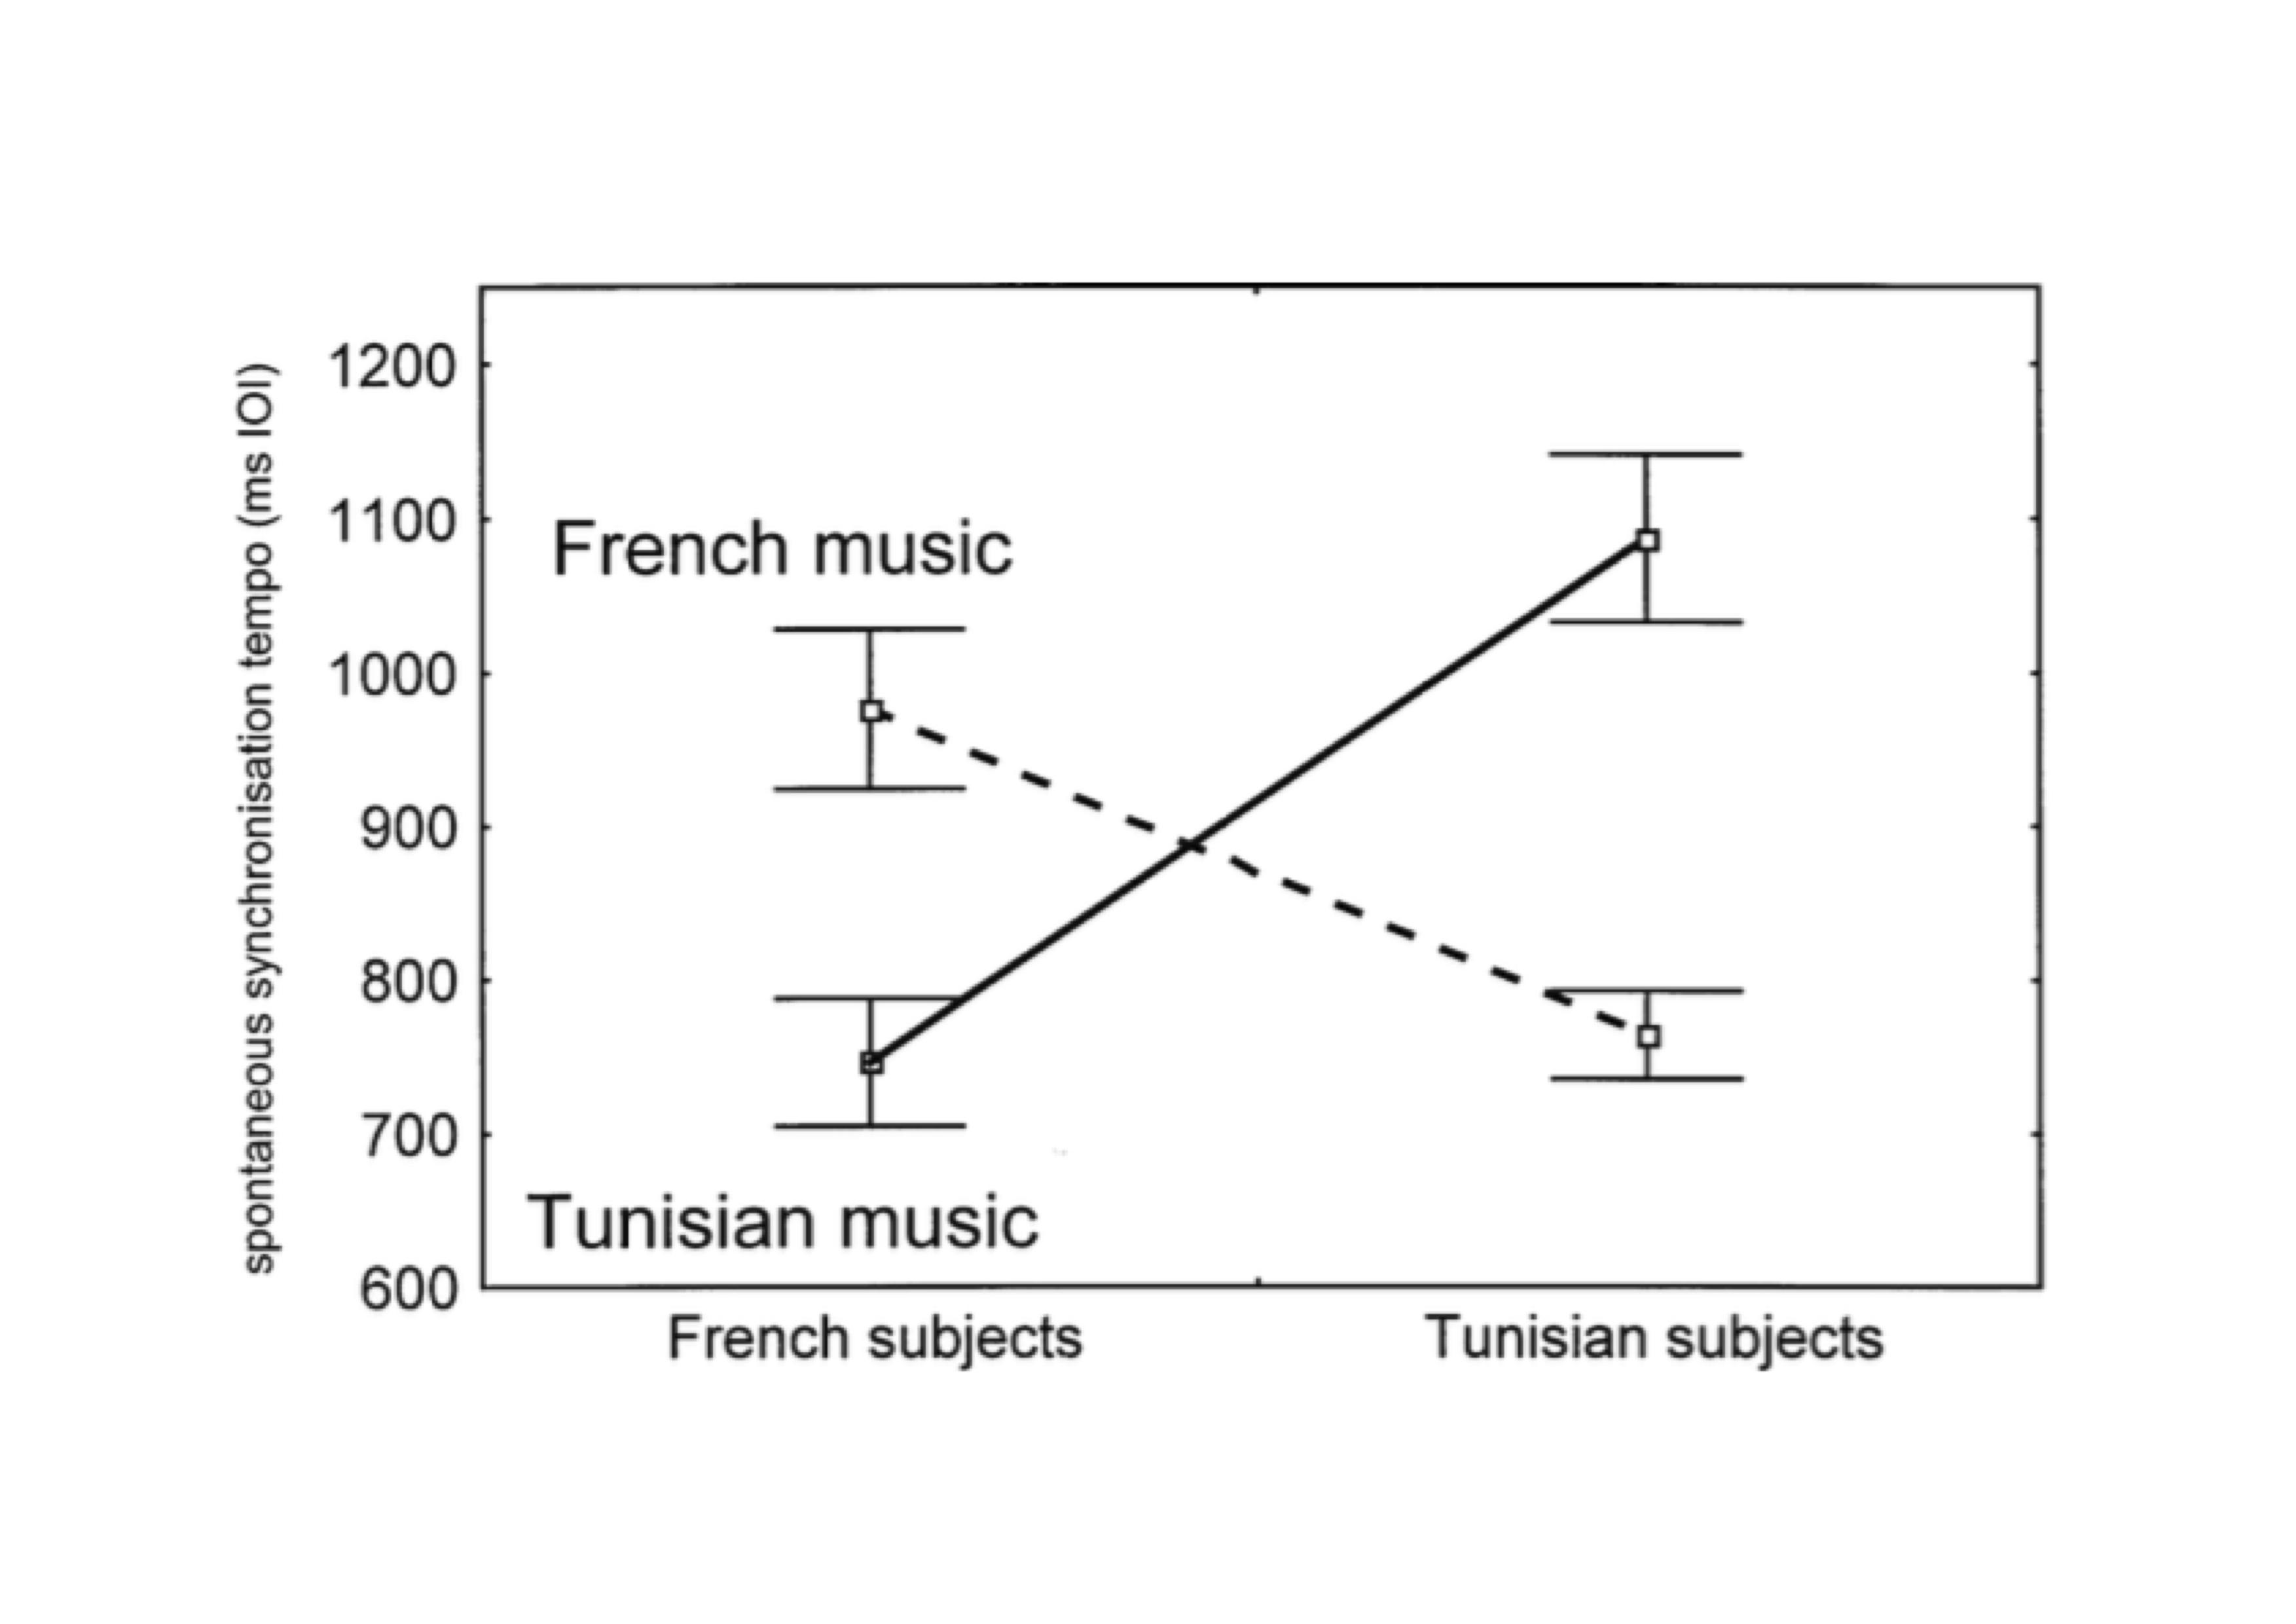
\includegraphics{figures/DrakeBenElHeni2003Fig2} 

}

\caption{Gemiddelde tijdsafstand tussen tikken (IOI, in ms) voor twee groepen luisteraars en twee muzieksoorten (ontleend aan Drake and Ben El Heni, 2003, Fig.2).}\label{fig:drakebenelheni2003fig2}
\end{figure}

\begin{quote}
Uit deze resultaten blijkt dat er géén verschil optreedt tussen de
groepen (Franse vs Tunesische luisteraars; de twee groepen hebben
gemiddeld dezelfde IOI), en dat er ook géén verschil optreedt tussen de
muzieksoorten (Franse vs Tunesische muziekstukken; de twee muzieksoorten
resulteren in gemiddeld dezelfde IOI). Hebben de twee onafhankelijke
variabelen dan geen enkel effect? Toch wel! De Franse luisteraars bleken
langere IOI's tussen tikken te produceren als ze naar Franse muziek
luisterden, terwijl de Tunesische luisteraars daarentegen langere IOI's
produceerden als ze naar Tunesische muziek luisterden. Alle luisteraars
blijken dus langere IOI's te produceren als ze luisteren naar een
muzieksoort die voor hen bekend is, en kortere IOI's als ze luisteren
naar een onbekende muzieksoort. \citet{Drake03} concluderen dat de luisteraars beter in
staat zijn om muzikale structuur te herkennen en te begrijpen in muziek
van hun eigen muzikale cultuur dan in die van een andere cultuur. Dit
patroon van resultaten is een klassiek kruislings interactie-effect,
waarbij het effect van de ene onafhankelijke variabele precies
tegengesteld is in de verschillende condities van de andere
onafhankelijke variabele.
\end{quote}

\begin{center}\rule{0.5\linewidth}{0.5pt}\end{center}

Als er een interactie-effect blijkt op te treden, dan is het zinloos om
een eventueel hoofdeffect te interpreteren. Dat werd al geïllustreerd in
Voorbeeld 6.5 hierboven: we kunnen niet concluderen dat er géén
verschil is tussen de muzieksoorten. Maar de grootte (en richting) van
het verschil is afhankelijk van de andere onafhankelijke variabele(n),
nl. van de groep/nationaliteit van de luisteraars. Veel onderzoek is er
juist op gericht om interactie-effecten aan te tonen; niet de
hoofdeffecten maar hun interactie vormt het onderwerp van onderzoek, net
als in het bovenstaande voorbeeld 6.5.

Een factorieel onderzoeksontwerp is lastig om schematisch weer te geven,
omdat er meerdere onafhankelijke variabelen (met elk weer meerdere
niveaus) in voorkomen. We zouden deze schematisch kunnen representeren
door de manipulatie, die we voorheen aangeduid hebben met een \texttt{X}, te
indiceren. De eerste index (subscript) geeft dan het niveau aan voor de
eerste onafhankelijke variabele of factor, en de tweede index geeft het
niveau aan van de tweede factor. Het ontwerp van voorbeeld 6.5 wordt dan als volgt schematisch weergegeven:

\begin{verbatim}
  R    X_{1,1}   O1
  R    X_{1,2}   O2
  R    X_{2,1}   O3
  R    X_{2,2}   O4
\end{verbatim}

Het is vaak verleidelijk om meerdere factoren te combineren in één groot
factorieel onderzoeksontwerp, zodat we kunnen onderzoeken hoe al die
factoren op elkaar inwerken (interageren). Toch is het verstandig om dat
\emph{niet} te doen, en om het aantal factoren beperkt te houden. Ten eerste,
zoals we later zullen zien, moet het aantal observaties ongeveer gelijke
tred houden met het aantal verschillende combinaties van factoren. Als
je meer combinaties van factoren toevoegt, dan zijn er daardoor ook veel
meer proefpersonen nodig (of andere eenheden). Ten tweede is het
moeilijker te garanderen dat alle combinaties van factoren perfect
vergelijkbaar zijn \citep[p.266]{SCC02}: zijn Tunesische deelnemers die in
Tunesië luisteren naar Tunesische muziek wel goed vergelijkbaar met
Franse deelnemers die in Frankrijk luisteren naar Franse muziek? De
vergelijkbaarheid van combinaties wordt lastiger, naarmate er meer
combinaties van factoren in het onderzoek voorkomen. Ten derde zijn
interacties notoir moeilijk te interpreteren, en dat wordt eveneens
lastiger naarmate de interacties complexer zijn, en meer factoren
omvatten. Om al deze redenen is het beter om effecten van meerdere
factoren te bestuderen in verschillende afzonderlijke onderzoeken
\citep{Quene10}.

We zullen later terugkomen op de analyse en interpretatie van gegevens
uit factoriële onderzoeksontwerpen
(Hoofdstuk \ref{ch:variantieanalyse}). Voorlopig concentreren we ons op
ontwerpen met slechts één onafhankelijke variabele.

\hypertarget{sec:afhankelijkegroepen}{%
\section{Afhankelijke- en onafhankelijke-groepen-ontwerp}\label{sec:afhankelijkegroepen}}

In het begin van dit hoofdstuk hebben we gesproken over de manipulatie
van een onafhankelijke variabele tussen danwel binnen proefpersonen ().
In de meeste van de voorafgaande onderzoeksontwerpen werd voor elke
waarde van de onafhankelijke variabele(n) een afzonderlijke groep
geformeerd; we noemen dat een onafhankelijke-groepen-ontwerp. De
onafhankelijke variabele varieert tussen proefpersonen.

Sommige onafhankelijke variabelen kunnen echter ook gevarieerd worden
binnen proefpersonen. We meten dan herhaaldelijk bij (binnen) dezelfde
proefpersonen uit dezelfde groep, onder verschillende condities van de
onafhankelijke variabele. In het onderstaande voorbeeld wordt de
onafhankelijke variabele `taal' (moedertaal of vreemde taal) gevarieerd
binnen proefpersonen. We noemen dat een afhankelijke-groepen-ontwerp.

\begin{center}\rule{0.5\linewidth}{0.5pt}\end{center}

\begin{quote}
\emph{Voorbeeld 6.6}:
\citep{JGSH13} onderzochten de vloeiendheid van de spraak van proefpersonen in hun
moedertaal (Turks) en in een vreemde taal (Nederlands). De proefpersonen
voerden eerst een aantal spreektaken uit in hun moedertaal, en enkele
weken later in het Nederlands. Eén van de afhankelijke variabelen was
het aantal gevulde pauzes (bijv. \emph{eh, ehm}) per seconde spraak: hoe meer
pauzes, hoe minder vloeiend. De sprekers bleken meer pauzes te
produceren (d.w.z. minder vloeiend te spreken) in de vreemde taal dan in
hun moedertaal, zoals ook te verwachten is. Eén van de doelen van het
onderzoek was overigens om te onderzoeken in hoeverre individuele
verschillen in vloeiendheid in de vreemde taal te herleiden zijn naar
individuele verschillen in vloeiendheid in de moedertaal. De samenhang
tussen de twee metingen bleek hoog (correlatie \(r=0.73\), meer hierover
in Hoofdstuk \ref{ch:samenhang}. Sprekers die veel pauzeren in de vreemde
taal, doen dat vaak ook in hun moedertaal. De onderzoekers bepleiten dat
met deze correlatie rekening gehouden moet worden bij het aanleren en
toetsen van spreekvaardigheid in een vreemde taal.
\end{quote}

Het hier beschreven onderzoeksontwerp ziet er in schema als volgt uit:

\begin{verbatim}
   X1   O1   X2   O2
\end{verbatim}

Ondanks de vele mogelijke bedreigingen van de interne validiteit (o.a.
geschiedenis, rijping, sturende werking van de voormeting) is zo'n
ontwerp in veel gevallen nuttig. In het bovenstaande voorbeeld is het
essentieel dat \emph{dezelfde} proefpersonen spreektaken uitvoeren in beide
talen (condities) --- de onderzoeksvragen zijn niet met een andere
methode te beantwoorden.

\hypertarget{onderzoek-ontwerpen}{%
\section{Onderzoek ontwerpen}\label{onderzoek-ontwerpen}}

Een onderzoeker die een onderzoek wil uitvoeren, moet bepalen op welke
wijze hij zijn gegevens gaat verzamelen: hij moet een keuze maken voor
een bepaald onderzoeksontwerp. Soms kan een standaard-ontwerp gekozen
worden, zoals een van de hierboven behandelde ontwerpen. In andere
gevallen zal de onderzoeker zelf het ontwerp moeten opstellen. Het
ontwerp moet uiteraard goed aansluiten bij de onderzoeksvraag
\citep{Levin99}, en het moet zoveel mogelijk storende variabelen uitsluiten
die de validiteit zouden kunnen bedreigen. Het ontwerpen van onderzoek
is een vak dat onderzoekers al doende leren. In het onderstaande
voorbeeld proberen we weer te geven welke redenering en argumenten een
rol spelen bij de ontwikkeling van een onderzoeksontwerp.

Stel je voor dat we willen onderzoeken of de vorm waarin toetsvragen
gesteld worden, als open vs.~gesloten vragen, van invloed is op de
scores op die toets. In een eenvoudig ontwerp nemen we eerst een toets
af met open vragen, en daarna een vergelijkbare toets met gesloten
vragen, bij dezelfde respondenten. Als de samenhang tussen de scores
hoog genoeg is, dan wordt geconcludeerd dat beide toetsen hetzelfde
meten, en dat de prestatie niet wezenlijk beïnvloed wordt door de vorm
waarin de vragen worden gesteld. Schematisch is dit ontwerp als volgt
weer te geven:

\begin{verbatim}
   Open   O1   Gesloten   O2
\end{verbatim}

Dit onderzoeksontwerp heeft echter diverse zwakke punten. Ten eerste is
het onverstandig om eerst alle toetsen met open vragen op het eerste
tijdstip af te nemen, en vervolgens alle toetsen met gesloten vragen op
het tweede tijdstip. De prestaties op de tweede toets worden immers
altijd beïnvloed door volgorde-effecten (transfer): de respondenten
hebben iets onthouden en dus geleerd van de eerste meting. Deze transfer
werkt nu altijd dezelfde kant op, met daardoor (vermoedelijk) relatief
hogere prestaties bij de toets met gesloten vragen (op het tweede
tijdstip). Het is dus beter om de toetsen met open en gesloten vragen
gelijkelijk te verdelen over het eerste en tweede tijdstip van afname.

Ten tweede kunnen alle respondenten beïnvloed zijn door eventuele
gebeurtenissen tussen de twee tijdstippen (geschiedenis), bijvoorbeeld
door een relevante instructie over het onderwerp van de toets. Omdat er
geen controle-groep is, kan met zo'n effect geen rekening worden
gehouden.

Een derde probleem is gelegen in de wijze waarop van bevindingen naar
conclusie wordt geredeneerd. Zoals gezegd, houdt die redenering in dat,
als de samenhang tussen de scores hoog genoeg is, dan beide toetsen
hetzelfde meten. Als je daarover nadenkt, dan ben je het misschien met
ons eens dat dat een vreemde redenering is. De onderzoeksvraag is
eigenlijk, of de samenhang in prestaties op verschillende toetsen met
verschillende vraagvormen even hoog is als de samenhang in prestaties op
verschillende toetsen met dezelfde vraagvormen, waarvan we immers
aannemen dat die hetzelfde meten. Daarmee hebben we in feite een
controle-groep gedefinieerd, nl. respondenten die op beide tijdstippen
toetsen maken met dezelfde vraagvorm. Voor alle zekerheid voegen we niet
één maar twee controle-groepen toe, met open resp. gesloten toetsvragen
op beide tijdstippen.

We hebben het ontwerp zo in tenminste twee opzichten verbeterd: (1) de open en gesloten
toetsen zijn gelijkelijk verdeeld over de twee opname-tijdstippen, en (2) er zijn
relevante controle-groepen toegevoegd. Schematisch ziet het
onderzoeksontwerp er nu als volgt uit:

\begin{verbatim}
       Exp. groep 1       Open     O1   Gesloten   O2
       Exp. groep 2     Gesloten   O3     Open     O4
      Controlegroep 1     Open     O5     Open     O6
      Controlegroep 2   Gesloten   O7   Gesloten   O8
\end{verbatim}

Voor alle vier de groepen kan nu de samenhang tussen de prestaties op
het eerste en tweede tijdstip bepaald worden. Vervolgens kunnen we deze
samenhang-resultaten uit de vier groepen vergelijken, en daarmee de
onderzoeksvraag beantwoorden. Dit voorbeeld laat goed zien dat de
conclusies die je uit de onderzoeksresultaten kunt trekken, direct
afhankelijk zijn van het gekozen ontwerp \citep{Levin99}. In het eerste
ontwerp leidt een lage gevonden samenhang tot de conclusie dat de twee
onderzochte toetsvormen \emph{niet} een beroep doen op dezelfde intellectuele
vaardigheden bij de respondenten. In het tweede ontwerp hoeft dezelfde
lage samenhang in de derde groep (experimentele groep 1) echter niet tot
dezelfde uitkomst te leiden! De conclusie hangt immers mede af van de
mate van samenhang gevonden in de andere groepen.

\hypertarget{tenslotte}{%
\section{Tenslotte}\label{tenslotte}}

Ondanks alle beschikbare boeken, handleidingen, websites, en ander
instructiemateriaal komen wij nog te vaak onderzoek tegen waar
methodologisch iets mis is in de onderzoeksvragen, operationalisatie,
onderzoeksopzet, steekproeftrekking, en/of dataverwerking. Die problemen
veroorzaken niet alleen een verspilling van tijd, geld en energie, maar
ze resulteren ook in kennis die minder betrouwbaar, valide en robuust is
dan mogelijk. De onderstaande `checklist' voor goed onderzoek (deels
ontleend aan
\url{https://www.linkedin.com/groups/4292855/4292855-6093149378770464768})
kan veel ellende in latere stadia van een onderzoek voorkomen.

\begin{enumerate}
\def\labelenumi{\arabic{enumi}.}
\item
  Denk goed na over je onderzoeksvragen, en formuleer ze helemaal uit.
  Als de vragen niet helder geformuleerd zijn, of als er veel
  deelvragen zijn, denk dan verder na.
\item
  Prioriteer de onderzoeksvragen. Dit helpt bij het maken van keuzes
  in onderzoeksontwerp, steekproeftrekking, operationalisatie, e.d.
\item
  Denk goed na over het ontwerp van het onderzoek. Volgens de
  overlevering levert ieder uur nadenken over je onderzoeksontwerp een
  toekomstige besparing van ongeveer 10 uren tijdens de data-analyse
  en interpretatie. Anders gezegd: een uur minder nadenken over je
  ontwerp kost je later 10 uur extra werk.
\item
  Bedenk ook alternatieve onderzoeksontwerpen, en denk na over de
  voordelen en nadelen van de diverse mogelijke ontwerpen.
\item
  Stel je de toekomst voor: je hebt het onderzoek uitgevoerd, de
  gegevens zijn geanalyseerd, en je hebt het verslag of de scriptie of
  het artikel geschreven. Welke boodschap wil je overbrengen op de
  lezers van dat verslag? Hoe draagt het onderzoeksontwerp bij aan die
  boodschap? Wat zou je kunnen veranderen in je ontwerp om die
  boodschap nog duidelijker te maken? Bedenk waar je naar toe wilt,
  niet alleen waar je nu staat.
\item
  Schrijf een onderzoeksplan, waarin je de verschillende
  methodologische aspecten beschrijft. Beargumenteer en expliciteer je
  onderzoeksvragen, onderzoeksontwerp, steekproef, meetmethode,
  data-verzameling, meetinstrumenten (bv. vragenlijst, software),
  andere benodigdheden (bv. laboratorium, vervoer), en statistische
  verwerking. Onderdelen van dit onderzoeksplan zijn later
  herbruikbaar in het onderzoeksverslag. Maak daarbij ook een
  tijdsplanning: wanneer zullen welke mijlpalen zijn bereikt?
\item
  Schrijf uit hoe je de verzamelde gegevens statistisch zult
  analyseren, nog voordat je begint met de eigenlijke
  data-verzameling. Wees daarbij weer zo expliciet mogelijk (in een
  script, stappenplan, o.i.d.). Maak een mini-dataverzameling van een
  redelijk aantal fictieve observaties of werkelijke observaties uit
  de pilot-fase van het onderzoek, en analyseer deze gegevens alsof
  het de definitieve data-verzameling betreft. Maak eventueel
  aanpassingen in je onderzoeksplan.
\item
  Als je eenmaal doende bent gegevens te verzamelen, maak dan \emph{geen}
  wijzigingen meer in het onderzoeksplan. Houd je aan dat plan en aan
  de bijbehorende tijdsplanning. Analyseer de gegevens op de wijze
  zoals vastgelegd in het (aangepaste) onderzoeksplan. Bespreek
  eventuele problemen die tijdens het onderzoek optraden wel in het
  onderzoeksverslag. Als er grote problemen optreden, breek dan het
  onderzoek af, en overweeg een verbeterde versie van je onderzoek.
\end{enumerate}

\hypertarget{ch:steekproeftrekking}{%
\chapter{Steekproeven}\label{ch:steekproeftrekking}}

Voor de generalisatie van de uitkomsten van een onderzoek naar de
doelgroep of de steekproef, is de kwaliteit van de steekproef bepalend.
Is de steekproef een adequate afspiegeling van de populatie? Om een
extreem voorbeeld te geven: als een steekproef bestaat uit meisjes in de
groep 8 van het basisonderwijs, dan kunnen de resultaten niet goed
gegeneraliseerd worden naar de populatie van alle basisschoolleerlingen,
want deze steekproef vormt geen goede afspiegeling van de populatie
basisschoolleerlingen (die immers bestaat uit jongens en meisjes van
alle groepen).

Afhankelijk van de methode die de onderzoekers gebruiken om de
proefpersonen te selecteren, kunnen er vele soorten steekproeven
onderscheiden worden. In dit hoofdstuk maken we een grove indeling in:
(1) gelegenheidssteekproeven, (2) systematisch getrokken steekproeven,
en (3) aselect of willekeurig (`at random') getrokken steekproeven. Voor
een verdere verdieping in de wijze waarop steekproeven getrokken kunnen
worden en de problemen die daarbij een rol spelen verwijzen we naar
standaardwerken hierover \citep{Coch77, Thom12}.

\hypertarget{sec:gelegenheidssteekproef}{%
\section{Gelegenheidssteekproeven}\label{sec:gelegenheidssteekproef}}

In veel sociaalwetenschappelijk onderzoek wordt gewerkt met steekproeven
die zich nu eenmaal aandienen, zogenaamde \emph{gelegenheidssteekproeven}. De
onderzoeker voert het experiment uit met personen die hem min of meer
toevallig ter beschikking staan. Voor sommige onderzoeken wordt gebruik
gemaakt van al dan niet betaalde vrijwilligers. In andere onderzoeken
worden studenten ingezet, die in het kader van hun studie verplicht zijn
een aantal uren als proefpersoon aan onderzoek mee te werken, of soms
moeten de studenten van een collega van de onderzoeker deelnemen aan het
onderzoek. Een dergelijke steekproef is niet zonder gevaren. De
onderzoeker heeft de mate van generaliseerbaarheid naar de populatie op
geen enkele manier meer in de hand. Natuurlijk heeft de onderzoeker wel
een populatie op het oog, en zal hij proefpersonen uit het onderzoek
weren die geen deel uit maken van de beoogde populatie (zoals
niet-moedertaal-sprekers), maar de onderzoeker kan geen uitspraken doen
over de representativiteit van de steekproef.

Met name in de psychologie heeft deze wijze van
gelegenheidssteekproeftrekking (`convenience sampling') aanleiding
gegeven tot verhitte discussies. Uit een telling bleek bijvoorbeeld dat
67\% van de steekproeven uit gepubliceerde Amerikaanse psychologische
studies uitsluitend bestond uit bachelor-studenten uit cursussen
Psychologie aan Amerikaanse universiteiten \citep{Henr10}. Dergelijke
steekproeven zijn natuurlijk verre van representatief. Gevolg daarvan is
dat de op deze gegevens gebaseerde theorieën slechts een beperkte
geldigheid hebben: de theorieën zouden vooral gelden voor het type
personen (westers, jong, hoog opgeleid, blank) dat ook in de
steekproeven sterk vertegenwoordigd is \citep{Henr10}. Ook in
taalwetenschappelijk onderzoek is de steekproef van proefpersonen
meestal een gelegenheidssteekproef. Kinderen die deelnemen als
proefpersoon hebben vaak hoogopgeleide ouders (niet zelden zelf
taalkundig geschoold, dus vermoedelijk bovengemiddeld verbaal begaafd),
en volwassen proefpersonen zijn vaak studenten uit de omgeving van de
onderzoekers, en dus ook bovengemiddeld hoog opgeleid en verbaal
begaafd.

Ondanks de steekhoudende bezwaren die tegen dit type steekproef naar
voren gebracht worden, dwingen de praktische omstandigheden vaak tot het
gebruik van een zich aandienende gelegenheidssteekproef. Wij bevelen dan
aan om na te gaan in hoeverre deze gelegenheidssteekproef zich
onderscheidt van de populatie waarover de onderzoeker wil generaliseren.
Tot slot van deze bespreking van zich aandienende steekproeven een
voorbeeld over de gevaren van dit type steekproef.

\begin{center}\rule{0.5\linewidth}{0.5pt}\end{center}

\begin{quote}
\emph{Voorbeeld 7.1}: Enige tijd geleden was er op televisie een wedstrijd te zien
over wie
van een negental kandidaten het beste kon zingen. De kijkers mochten hun
voorkeur telefonisch kenbaar maken. Voor alle negen kandidaten was een
aparte telefoonlijn geopend. Voor elke beller kreeg een kandidaat één
punt. Degene die de meeste punten binnen een bepaalde tijdlimiet
verzameld had was de winnaar. De reactie van het publiek was
overweldigend: in grote delen van Nederland was het telefoonnet volledig
overbezet. Al snel bleek één van de kandidaten een flinke voorsprong te
hebben. In de loop van de avond werd deze voorsprong echter steeds
kleiner. Uiteindelijk scheelde het nog maar enkele bellers met nummer
twee. Opvallend was overigens dat naarmate de avond vorderde de
verschillen tussen de deelnemers (relatief) steeds kleiner werden.
\end{quote}

\begin{center}\rule{0.5\linewidth}{0.5pt}\end{center}

We kunnen deze stemprocedure beschouwen als een trekking van een
steekproef van bellers c.q. stemmers. Deze steekproef is echter verre
van representatief. Als veel kiezers willen stemmen op één kandidaat,
dan zal de telefoonlijn voor die kandidaat overbezet raken. Dus: de
zangers die veel bellers trekken, zullen relatief minder stemmen krijgen
dan zangers die weinig bellers trekken, omdat de telefoonlijnen van de
laatsten niet overbezet zullen zijn. Juist bij de populairste kandidaten
is de kans het grootst dat een kiezer zijn stem \emph{niet} kan laten gelden.
In werkelijkheid zal er dus een veel groter verschil zijn in aantal
stemmen per kandidaat, dan de organisator gemeten heeft. De organisator
heeft deze systematische vertekening (bias) van de resultaten helaas
zelf veroorzaakt, door voor elk van de negen kandidaten een eigen
telefoonlijn te openen. De gegevens hadden veel representatiever kunnen
zijn, als de organisator negen telefoonlijnen had geopend, met één
gemeenschappelijk toegangsnummer. De steekproef van bellers die hun stem
kunnen uitbrengen is dan representatief voor de populatie van alle
bellers, en dat was nu niet het geval.

\hypertarget{sec:systematischesteekproef}{%
\section{Systematische steekproeven}\label{sec:systematischesteekproef}}

Wanneer de elementen in de \emph{steekproefruimte} (d.i. de verzameling van
mogelijke elementen in een steekproef) op de een of andere manier
systematisch geordend zijn, dan kan met behulp van een \emph{systematische
trekkingsprocedure} van steekproefelementen een redelijk representatieve
steekproef verkregen worden. Een ordening kan zijn bijvoorbeeld een
namenlijst.

\begin{center}\rule{0.5\linewidth}{0.5pt}\end{center}

\begin{quote}
\emph{Voorbeeld 7.2}:Laten we even aannemen dat we een onderzoek willen doen naar de
taalvaardigheid van derdeklassers in het voortgezet onderwijs. De gehele
populatie van derdeklassers is echter veel te groot om van alle
derdeklassers de taalvaardigheid te meten (lezen, schrijven, spreken, en
luisteren). In de derde klas zitten namelijk ongeveer 200.000
leerlingen. Er moet dus een steekproef genomen worden. Op het Ministerie
van Onderwijs, Cultuur en Wetenschappen is een registratiesysteem
beschikbaar waarin een lijst met de namen van alle scholen met derde
klassen is opgenomen. Een voor de hand liggende werkwijze is nu deze
lijst te nemen en elke 100ste school van die lijst in de steekproef op
te nemen. Deze werkwijze resulteert vermoedelijk in een tamelijk
representatieve steekproef.
\end{quote}

\begin{center}\rule{0.5\linewidth}{0.5pt}\end{center}

Twee factoren kunnen echter roet in het eten gooien bij zo'n
systematische steekproef: ten eerste de \emph{responsiegraad}. Als een
aanzienlijk deel van de aangeschreven scholen geen medewerking verleent,
dan hebben we in feite te maken met zelf-selectie (zie
§\ref{sec:internevaliditeit} punt 5)
en dus met een zichzelf aandienende
gelegenheidssteekproef (zie
§\ref{sec:gelegenheidssteekproef}). Dat is een ongewenste
situatie, want de scholen die wel meewerken hebben vermoedelijk een
grotere `plichtsgetrouwheid' dan de weigerende scholen of dan de
gemiddelde school. Bovendien kunnen de leerlingen op de responderende en
niet-responderende scholen van elkaar verschillen
(zie §\ref{sec:internevaliditeit} punt 5).
De uiteindelijke steekproef is dan
misschien niet meer representatief voor de populatie van alle
derdeklassers. Het gevolg daarvan is weer dat de gemeten resultaten
slecht generaliseerbaar zijn naar andere derdeklassers van andere
scholen.

De tweede factor die de representativiteit van een systematische
steekproef kan beïnvloeden is de \emph{storende trendwerking}. Er is sprake
van een storende trendwerking wanneer populatie-elementen met een
bepaald relevant kenmerk meer kans hebben in de steekproef terecht te
komen dan populatie-elementen die dit kenmerk niet hebben. In ons
voorbeeld van de meting van de taalvaardigheid van derdeklassers hebben
we met de storende trendwerking te maken. Niet alle leerlingen hebben
namelijk een gelijke kans om in de steekproef te komen. Immers, elke
individuele \emph{school} (niet: leerling) heeft dezelfde kans als elke
andere school om in de steekproef terecht te komen. Het gevolg is dat er
relatief meer derdeklassers in de steekproef zullen komen van kleine
scholen met relatief weinig leerlingen, en omgekeerd relatief minder
derdeklassers van grote scholen met relatief veel leerlingen.
Derdeklassers van grote scholen zijn ondervertegenwoordigd. Is dat erg?
Misschien wel, want de taalvaardigheid (afhankelijke variabele) wordt
deels beïnvoed door de vorm van onderwijs, en die onderwijsvorm wordt
weer beïnvloed door de grootte van de school. De hierboven beschreven
steekproef is dus niet representatief voor de populatie van
derdeklassers. Wederom is het gevolg dat de gemeten resultaten slecht
generaliseerbaar zijn naar andere derdeklassers van andere scholen.

\hypertarget{sec:aselectesteekproef}{%
\section{Aselecte steekproeven}\label{sec:aselectesteekproef}}

De hierboven beschreven storende trendwerking kunnen we voorkomen door
random of \emph{aselecte steekproeftrekking}. Aselecte steekproeftrekking kan
op diverse manieren gebeuren, waarvan we er hier drie bespreken.

De eerste vorm is \emph{simple random sampling}: hierbij krijgen alle
elementen van de populatie een gelijke kans om getrokken te worden. Dit
kan bijvoorbeeld gerealiseerd worden door alle elementen van een
\emph{random} nummer te voorzien en dan, afhankelijk van de gewenste
steekproefgrootte, steeds het \(n\)-de element te selecteren. Voor de
selectie van getallen staan de onderzoeker tabellen met toevalsgetallen
ter beschikking (zie Appendix \ref{app:randomgetallen}).
Ook rekenmachines, computers,
spreadsheet-programma's e.d. kunnen random getallen genereren (zie secties hieronder).
Het verdient aanbeveling om zulke random getallen te gebruiken, want een
door mensen geconstrueerde ``random'' volgorde is niet werkelijk
``random''. Een voorwaarde voor de toepassing van deze methode is echter
wel dat de elementen van de populatie (steekproefruimte) vooraf
geregistreerd zijn (of worden), zodat ze op enigerlei wijze van een
nummer voorzien kunnen worden.

\begin{center}\rule{0.5\linewidth}{0.5pt}\end{center}

\begin{quote}
\emph{Voorbeeld 7.3}: We willen een steekproef trekken
van \(n=400\) basisscholen. Dit is ongeveer 4\% van de populatie van
basisscholen. We vragen daarom bij het Ministerie van Onderwijs, Cultuur
en Wetenschappen een lijst met alle 9000 basisscholen op; deze lijst
vormt de steekproefruimte. Vervolgens voorzien we alle basisscholen van
een volgnummer \((1, 2, 3, \ldots, 9000)\). Tenslotte selecteren we alle
basisscholen waarvan de laatste twee cijfers \emph{toevallig} 36 of 43 of 59
of 70 zijn (zie Appendix \ref{app:randomgetallen}, eerste kolom, laatste twee cijfers).
Met deze procedure selecteren we volgens het toeval 4 van de 100
mogelijke laatste-twee-cijfer-combinaties, ofwel 4\% van de scholen.
\end{quote}

\begin{center}\rule{0.5\linewidth}{0.5pt}\end{center}

De tweede vorm van aselecte steekproeftrekking is
\emph{stratified random sampling}.
Daarvan is sprake als we van elk populatie-element de waarde
van een kenmerk weten (bv. religieuze denominatie), en als we zorgen dat
in de steekproef de elementen evenredig verdeeld zijn volgens dit
kenmerk. We verdelen de steekproef daarvoor in zogenaamde `strata' of
lagen (Lat. \emph{stratum}, `bedekking, laag', verwant aan Ned. \emph{straat},
`verharde weg'). Terug naar de basisschool om het een en ander te
verhelderen. Om welke reden dan ook zijn we er nu in geïnteresseerd de
steekproef (nog steeds 4\% van de populatie van basisscholen) zo te maken
dat openbare, katholieke en protestante scholen in gelijke mate
vertegenwoordigd zijn. We stellen daarom drie lijsten op: voor alle drie
de schooltype een aparte lijst. Binnen iedere lijst gaan we net zo te
werk als bij simple random sampling. Uiteindelijk worden de drie
deel-steekproeven van de drie strata gecombineerd.

Met \emph{quota sampling} gaan we nog een stapje verder dan bij `stratified
random sampling': we verdisconteren nu ook het feit dat we weten wat de
verdeling is van een bepaald kenmerk (bv denominatie) in de populatie.
Uit de lijst met basisscholen zou hebben kunnen blijken dat 35\% van de
scholen openbaar is, 31\% katholiek, 31\% protestant en dat 3\% een andere
signatuur heeft. We trekken uit de steekproefruimte nu meerdere aselecte
`stratified' steekproeven, en wel zo dat de verhouding van scholen in de
strata een juiste afspiegeling vormt van de verhoudingen van dit kenmerk
in de steekproefruimte \((35:31:31:3)\).

\hypertarget{spss}{%
\subsection{SPSS}\label{spss}}

Voor het aanmaken van een kolom met random getallen:

\begin{verbatim}
Transform > Compute...
\end{verbatim}

Selecteer een bestaande variabele (sleep naar Variable(s) paneel) of geef de naam voor een nieuwe variabele.
Uit het paneel ``Function Group'', kies ``Random Numbers'' en daarna \texttt{RV.UNIFORM}.
Deze functie kiest aselect (\textbf{r}andom) waarden (\textbf{v}alues) uit een vlakke (\textbf{uniform}e) kansverdeling, d.w.z. dat elk getal tussen de ondergrens en bovengrens een gelijke kans heeft om getrokken te worden.
Kies als ondergrens \texttt{0} en als bovengrens \texttt{9999}, of andere grenzen naar behoefte.
Bevestig met \texttt{OK}.\\
Dit resulteert in een (nieuwe, of overschreven bestaande) kolom met random getallen.

Als je random getallen wilt genereren volgens een normale kansverdeling (zie Hoofdstuk \ref{ch:kansverdelingen}), gebruik dan de functie \texttt{RV.NORMAL(mean,stdev)}.

We kunnen een eigen beginwaarde meegeven aan de ``random number generator'', om zo reproduceerbare analyses te kunnen maken:

\begin{verbatim}
Transform > Random Number Generators...
\end{verbatim}

Vink in het paneel ``Active Generator Initialization'' de optie \texttt{Set\ Starting\ Point} aan, en vul een eigen beginwaarde in, bijvoorbeeld je lievelingsgetal. Bevestig met \texttt{OK}.

Je kunt deze random getallen gebruiken om op aselecte wijze eenheden (bijv. proefpersonen) te kiezen voor een steekproef, maar uiteraard ook om op aselecte wijze de geselecteerde eenheden toe te wijzen aan condities, enzovoort.

\hypertarget{r}{%
\subsection{R}\label{r}}

In R kunnen we random getallen genereren met de functie \texttt{runif}. Deze functie kiest aselect (\textbf{r}andom) waarden uit een vlakke (\textbf{unif}orme) kansverdeling, d.w.z. dat elk getal tussen de ondergrens en bovengrens een gelijke kans heeft om getrokken te worden. De standaard grenzen zijn \((0,1)\). De waarden kunnen we afronden tot gehele getallen, zoals gedaan is voor Appendix \ref{app:randomgetallen}.

Als je random getallen wilt genereren volgens een normale kansverdeling (zie Hoofdstuk \ref{ch:kansverdelingen}), gebruik dan de functie \texttt{rnorm(n,mean,sd)}.

Met de opdracht \texttt{set.seed} geven we een eigen beginwaarde mee aan de ``random number generator'', om zo reproduceerbare analyses (en demonstraties) te kunnen maken.

\begin{Shaded}
\begin{Highlighting}[]
\KeywordTok{set.seed}\NormalTok{(}\DecValTok{20200912}\NormalTok{) }\CommentTok{\# reproduceerbaar voorbeeld (bijv datum als getal)}
\KeywordTok{round}\NormalTok{ ( }\KeywordTok{runif}\NormalTok{( }\DataTypeTok{n=}\DecValTok{5}\NormalTok{, }\DataTypeTok{min=}\DecValTok{0}\NormalTok{, }\DataTypeTok{max=}\DecValTok{9999}\NormalTok{ ) )}
\end{Highlighting}
\end{Shaded}

\begin{verbatim}
## [1] 8193 7482 4206 1684 5653
\end{verbatim}

Je kunt deze random getallen gebruiken om op aselecte wijze eenheden (bijv. proefpersonen) te kiezen voor een steekproef, maar uiteraard ook om op aselecte wijze de geselecteerde eenheden toe te wijzen aan condities, enzovoort.

\hypertarget{sec:steekproefgrootte}{%
\section{Steekproefgrootte}\label{sec:steekproefgrootte}}

Als je verschillende onderzoeksartikelen leest, dan is één van de eerste
zaken die opvalt de enorme variatie in aantallen respondenten. In
sommige onderzoeken worden enkele duizenden proefpersonen betrokken en
in andere slechts enkele tientallen of soms nog minder. We zullen hier
twee aspecten bespreken die van invloed zijn op de vereiste grootte van
de steekproef: de homogeniteit van de populatie, en de aard van de
steekproeftrekking. In volgende hoofdstukken zullen we nog twee andere
aspecten bespreken die eveneens van invloed zijn op de gewenste
steekproefgrootte, nl. de gewenste precisie (effectgrootte,
§\ref{sec:ttoets-effectgrootte}) en de gewenste kans om een effect
aan te tonen als dat in de populatie ook daadwerkelijk aanwezig is
(power,
§\ref{sec:effectgrootte-power}).

\begin{center}\rule{0.5\linewidth}{0.5pt}\end{center}

\begin{quote}
\emph{Voorbeeld 7.4}: Wanneer auto's getest worden (in een
tijdschrift of op televisie), dan wordt van een type auto slechts één
exemplaar getest. De resultaten van dit testexemplaar worden zonder
voorbehoud gegeneraliseerd naar alle auto's van hetzelfde type en merk.
Dit is mogelijk omdat de populatie auto's waarnaar gegeneraliseerd wordt
bijzonder homogeen is: de fabrikant streeft er immers naar om de
verschillende exemplaren zo gelijk mogelijk op de markt te brengen.
\end{quote}

\begin{center}\rule{0.5\linewidth}{0.5pt}\end{center}

De vereiste steekproefgrootte hangt ten eerste af van de homogeniteit
van de populatie. Als een populatie \emph{homogeen} is, zoals de auto's in
voorbeeld 7.4 hierboven, dan kunnen we met een kleine
steekproef volstaan. Anders is het wanneer we bijvoorbeeld de
conversatiepatronen van kleuters willen analyseren. In de
conversatiepatronen van kleuters treffen we grote verschillen aan; er is
een zeer grote variatie in conversatiepatronen. (Sommige kinderen praten
voluit, en andere zwijgen vooral. Bovendien zijn er grote individuele
verschillen in taalontwikkeling tussen kinderen.) Om een goed beeld te
krijgen van de taalontwikkeling van kleuters, hebben we daarom een veel
grotere steekproef nodig. De grootte van de benodigde steekproef neemt
dus toe naarmate de populatie waarna gegeneraliseerd moet worden minder
homogeen (heterogener) is.

Ten tweede hangt de vereiste steekproefgrootte ook af van de aard van de
steekproef. Als er in een populatie duidelijke strata aanwezig zijn,
maar we passen -- om welke reden dan ook -- geen `stratified' of `quota
sampling' toe, dan hebben we een grotere steekproef nodig dan wanneer we
dit wel zouden doen. Immers, bij deze laatste twee methoden zorgt de
onderzoeker zelf voor een gelijke dan wel evenredige vertegenwoordiging
van strata in de steekproef, maar bij `simple random sampling' wordt dat
aan het toeval overgelaten. We doen dan dus een beroep op de ``wet van de
grote getallen'' om te zorgen dat er voldoende elementen uit de
verschillende strata in de steekproef terecht komen, om generalisatie
van de resultaten naar die verschillende strata te rechtvaardigen.
Uiteraard werkt die wet alleen bij een voldoende grote steekproef! Bij
een kleine steekproef weten we allerminst zeker dat de verschillende
strata in voldoende mate in de steekproef vertegenwoordigd zijn.

Als we, om naar het basisschool-voorbeeld terug te keren, drie
basisscholen zouden selecteren volgens `simple random sampling', dan
bestaat natuurlijk een kans dat dit precies één openbare, één katholieke
en één protestante school oplevert in deze steekproef. Maar ook andere
uitkomsten zijn zeer reëel, en zelfs meer waarschijnlijk. Bij
`stratified' en `quota sampling' hebben we gegarandeerd van elke
denominatie één element (school) in onze steekproef. Onze basis voor
generalisatie is beter, en de externe validiteit is dus sterker.

Na al deze behartenswaardige aanbevelingen wordt het tijd om te
bespreken hoe we onderzoeksgegevens goed kunnen beschrijven en
analyseren om onze onderzoeksvragen te beantwoorden. Dat gebeurt in het
volgende deel van dit boek.

\hypertarget{part-deel-ii-beschrijvende-statistiek}{%
\part*{Deel II: Beschrijvende statistiek}\label{part-deel-ii-beschrijvende-statistiek}}
\addcontentsline{toc}{part}{Deel II: Beschrijvende statistiek}

\hypertarget{ch:frequenties}{%
\chapter{Frequenties}\label{ch:frequenties}}

\hypertarget{inleiding-3}{%
\section{Inleiding}\label{inleiding-3}}

Bij de analyse van gegevens wordt vaak een onderscheid gemaakt tussen
kwalitatieve danwel kwantitatieve methoden. Bij de eerste methode worden
waarnemingen (bijv. antwoorden in interviews) gerepresenteerd in
woorden, en bij de tweede methode worden waarnemingen (bijv.
spreekpauzes in interviews) gerepresenteerd in getallen. Naar onze
mening bestaat het verschil tussen kwalitatieve en kwantitatieve
methoden dus uit de aard van de representatie van de observaties, en
daarmee uit de wijze van argumentatie op grond van die observaties. Soms
is het ook mogelijk om dezelfde gegevens (bijv. interviews) zowel
kwalitatief als kwantitatief te analyseren. De kwantitatieve methode
heeft als grote voordelen dat de gegevens relatief eenvoudig samengevat
kunnen worden (daarover gaat dit deel van het tekstboek), en dat het
relatief makkelijk is om zinvolle conclusies te trekken op basis van de
observaties.

\hypertarget{sec:frequenties}{%
\section{Frequenties}\label{sec:frequenties}}

Kwantitatieve gegevens kunnen op allerlei manieren gerapporteerd worden.
De eenvoudigste manier zou zijn om de ruwe gegevens te rapporteren, bij
voorkeur gesorteerd naar de waarde van de geobserveerde variabele.
Nadeel daarvan is dat een eventueel patroon in de observaties niet goed
zichtbaar wordt.

\begin{center}\rule{0.5\linewidth}{0.5pt}\end{center}

\begin{quote}
\emph{Voorbeeld 8.1}: Studenten \((N=50)\) in een eerstejaars
cursus rapporteerden de volgende waarden voor hun schoenmaat, een
variabele van het interval-meetniveau:\\
36, 36, 37, 37, 37, 37, 37, 37, 38, 38, 38, 38, 38, 38, 39, 39, 39, 39,
39, 39, 39, 39, 39, 39, 39, 39, 39, 39, 39, 39, 39, 39, 39, 40, 40, 40,
40, 40, 40, 41, 41, 41, 41, 41, 42, 42, 43, 43, 44, ??.\\
Eén van de studenten heeft geen antwoord opgegeven; dit ontbrekende
antwoord is hier aangegeven als ??.
\end{quote}

\begin{center}\rule{0.5\linewidth}{0.5pt}\end{center}

Meestal is het inzichtelijker en efficiënter om de observaties samen te
vatten en te rapporteren in de vorm van de \emph{frequentie} van elke waarde.
Die frequentie geeft het \emph{aantal} observaties met een bepaalde waarde,
of met een waarde in een bepaald interval of klasse. Om de frequentie te
verkrijgen \emph{tellen} we dus het aantal observaties met een bepaalde
waarde, of het aantal observaties in een bepaald interval. Deze
frequenties worden gerapporteerd in een tabel. Zo'n tabel wordt een
frequentieverdeling genoemd (frequency distribution).

Tabel \ref{tab:klankfreq} geeft als eerste voorbeeld een
frequentieverdeling van een discrete variabele van \emph{nominaal}
meetniveau, nl. de fonologische klasse van spraakklanken in het
Nederlands \citep{LKCG07}.

\begin{table}

\caption{\label{tab:klankfreq}Frequentieverdeling 
              van fonologische klasse van spraakklanken 
              in het *Corpus Gesproken Nederlands* 
              (C=consonant=medeklinker, V=vocaal=klinker).}
\centering
\begin{tabular}[t]{llr}
\toprule
hoofdklasse & onderklasse & aantal\\
\midrule
C & plos & 585999\\
C & fric & 426097\\
C & liq & 249275\\
C & nas & 361742\\
C & glide & 146344\\
\addlinespace
V & lang & 365887\\
V & kort & 428832\\
V & schwa & 341260\\
V & diph & 61638\\
V & rest & 1146\\
\bottomrule
\end{tabular}
\end{table}

Tabel \ref{tab:schoenmaat} geeft als tweede voorbeeld een
frequentieverdeling van een continue variabele van \emph{interval}
meetniveau, nl. de al eerder genoemde schoenmaat van eerstejaars
studenten (Voorbeeld 8.1).

\begin{longtable}[]{@{}lcccccccccc@{}}
\caption{\label{tab:schoenmaat} Frequentieverdeling van zelfgerapporteerde schoenmaten
van \(N=50\) studenten in een eerstejaars cursus (zie
Voorbeeld 8.1 hierboven).}\tabularnewline
\toprule
\endhead
Schoenmaat & 36 & 37 & 38 & 39 & 40 & 41 & 42 & 43 & 44 & ??\tabularnewline
Aantal & 2 & 6 & 6 & 19 & 6 & 5 & 2 & 2 & 1 & 1\tabularnewline
\bottomrule
\end{longtable}

Als een numerieke variabele heel veel verschillende waarden kan
aannemen, dan wordt de frequentieverdeling op deze manier toch groot en
onoverzichtelijk. We voegen dan waarden in een bepaald interval bij
elkaar, en maken daarna een frequentieverdeling over dat geringere
aantal intervallen of klassen.

\begin{center}\rule{0.5\linewidth}{0.5pt}\end{center}

\begin{quote}
\emph{Voorbeeld 8.2}: Toen Koningin Beatrix voor het laatst de Troonrede voorlas,
op 18 september 2012, pauzeerde ze daarbij \(305\times\). De frequentieverdeling
van de duur van de pauze (gemeten in seconden) is weergegeven in
Tabel \ref{tab:troonrede2012pauzes}.
\end{quote}

\begin{center}\rule{0.5\linewidth}{0.5pt}\end{center}

\begin{longtable}[]{@{}cr@{}}
\caption{\label{tab:troonrede2012pauzes} Frequentieverdeling van de duren van spreekpauzes (in seconden) in de Troonrede van 18 september 2012, voorgelezen door Koningin Beatrix \((N=305)\).}\tabularnewline
\toprule
Interval & Aantal\tabularnewline
\midrule
\endfirsthead
\toprule
Interval & Aantal\tabularnewline
\midrule
\endhead
4.50--4.99 & 1\tabularnewline
4.00--4.49 & 0\tabularnewline
3.50--3.99 & 2\tabularnewline
3.00--3.49 & 7\tabularnewline
2.50--2.99 & 4\tabularnewline
2.00--2.49 & 25\tabularnewline
1.50--1.99 & 32\tabularnewline
1.00--1.49 & 16\tabularnewline
0.50--0.99 & 67\tabularnewline
0.00--0.49 & 151\tabularnewline
\bottomrule
\end{longtable}

\hypertarget{sec:intervallen}{%
\subsection{Intervallen}\label{sec:intervallen}}

Voor een variabele van nominaal en ordinaal meetniveau gebruiken we
doorgaans de oorspronkelijke categorieën om de frequentieverdeling te
maken (zie Tabel \ref{tab:klankfreq}), al is het wel mogelijk om categorieën samen
te voegen. Voor een variabele van interval- of ratio-meetniveau kan een
onderzoeker zelf het aantal intervallen in de frequentieverdeling
kiezen. Soms is dat niet nodig, bijvoorbeeld omdat de variabele een
overzichtelijk aantal verschillende discrete waarden heeft (zie
Tabel \ref{tab:schoenmaat}). Maar soms sta je als onderzoeker
voor de keuze hoeveel intervallen te onderscheiden, en hoe de grenzen
van die intervallen te bepalen (zie Tabel \ref{tab:troonrede2012pauzes}).
Daarbij gelden dan de volgende aanbevelingen \citep[Ch.2]{Ferg89}:

\begin{itemize}
\item
  Zorg dat alle observaties (d.w.z. het gehele bereik) vallen binnen
  ruwweg 10 tot 20 intervallen.
\item
  Zorg dat alle intervallen even breed zijn.
\item
  Laat de ondergrens van het eerste of tweede interval samenvallen met
  de breedte van de intervallen (zie
  Tabel \ref{tab:troonrede2012pauzes}: ieder interval is 0.50 s
  breed, en de ondergrens van het tweede interval is ook 0.50).
\item
  Orden de intervallen in een frequentieverdeling van beneden naar
  boven in toenemende volgorde (d.i. van boven naar beneden in
  afnemende volgorde, Eng. descending), zie
  Tabel \ref{tab:troonrede2012pauzes}).
\end{itemize}

Naarmate we de intervallen breder maken, verliezen we meer informatie
over de precieze verdeling binnen elk interval.

\hypertarget{spss-1}{%
\subsection{SPSS}\label{spss-1}}

\begin{verbatim}
Analyze > Descriptive Statistics > Frequencies...
\end{verbatim}

Selecteer variabele (sleep naar paneel ``Variable(s)'').\\
Vink aan: \texttt{Display\ frequency\ tables}.\\
Kies \texttt{Format}, kies: \texttt{Order\ by:\ Descending\ values}.\\
Bevestig met \texttt{OK}.\\

\hypertarget{r-1}{%
\subsection{R}\label{r-1}}

\begin{Shaded}
\begin{Highlighting}[]
\NormalTok{enq2011 \textless{}{-}}\StringTok{ }\KeywordTok{read.table}\NormalTok{( }
    \DataTypeTok{file=}\KeywordTok{url}\NormalTok{(}\StringTok{"http://www.hugoquene.nl/R/enq2011.txt"}\NormalTok{), }
    \DataTypeTok{header=}\OtherTok{TRUE}\NormalTok{ )}
\KeywordTok{table}\NormalTok{( enq2011}\OperatorTok{$}\NormalTok{schoen, }\DataTypeTok{useNA=}\StringTok{"ifany"}\NormalTok{ ) }
\end{Highlighting}
\end{Shaded}

De uitvoer van bovenstaande \texttt{table} commando is weergegeven in Tabel \ref{tab:schoenmaat}.
De code \texttt{NA} (Not Available) wordt in R gebruikt om ontbrekende gegevens aan te duiden.

\begin{Shaded}
\begin{Highlighting}[]
\CommentTok{\# lees dataset }
\KeywordTok{load}\NormalTok{(}\DataTypeTok{file=}\StringTok{"data/pauses6.Rda"}\NormalTok{)}
\CommentTok{\# haal daaruit pauzeduren (kolom 12) voor jaar 2012, in aparte variabele \textasciigrave{}troon2012\textasciigrave{}}
\NormalTok{troon2012 \textless{}{-}}\StringTok{ }\NormalTok{pauses6[ pauses6}\OperatorTok{$}\NormalTok{jaar}\OperatorTok{==}\DecValTok{2012}\NormalTok{, }\DecValTok{12}\NormalTok{ ] }\CommentTok{\# save col\_12 as single vector}
\end{Highlighting}
\end{Shaded}

\begin{Shaded}
\begin{Highlighting}[]
\KeywordTok{table}\NormalTok{( }\KeywordTok{cut}\NormalTok{( troon2012, }\DataTypeTok{breaks=}\KeywordTok{seq}\NormalTok{(}\DataTypeTok{from=}\DecValTok{0}\NormalTok{,}\DataTypeTok{to=}\DecValTok{5}\NormalTok{,}\DataTypeTok{by=}\FloatTok{0.5}\NormalTok{) ) )}
\end{Highlighting}
\end{Shaded}

Ontleed bovenstaande opdracht vanuit de binnenste haakjes naar buiten:
(i) \texttt{seq}: maak een reeks (sequence) van 0 tot 5 (eenheden, hier: seconden) in stappen van 0.5 seconden,
(ii) \texttt{cut}: hak de afhankelijke variabele \texttt{troon2012} (duren van pauzes in de Troonrede van 2012) op in intervallen op basis van deze reeks,
(iii) \texttt{table}: maak een frequentieverdeling van deze intervallen.

De uitvoer van deze laatste opdracht is weergegeven (in aangepaste vorm) in Tabel \ref{tab:troonrede2012pauzes}, en wordt hier onderdrukt.

\hypertarget{sec:staafdiagrammen}{%
\section{Staafdiagrammen}\label{sec:staafdiagrammen}}

Een staafdiagram (Eng. `bar chart') is de grafische weergave van de
frequentieverdeling van een discrete, categorische variabele (van
nominaal of ordinaal meetniveau). Een staafdiagram is opgebouwd uit
rechthoeken. Alle rechthoeken zijn even breed, en de hoogte van de
rechthoek correspondeert met de frequentie van die categorie. De
oppervlakte van iedere rechthoek correspondeert dus ook met de
frequentie van die categorie. In tegenstelling tot een histogram sluiten
de rechthoeken \emph{niet} op elkaar aan langs de horizontale as, om aan te
geven dat we te maken hebben met discrete categorieën.

\begin{figure}
\centering
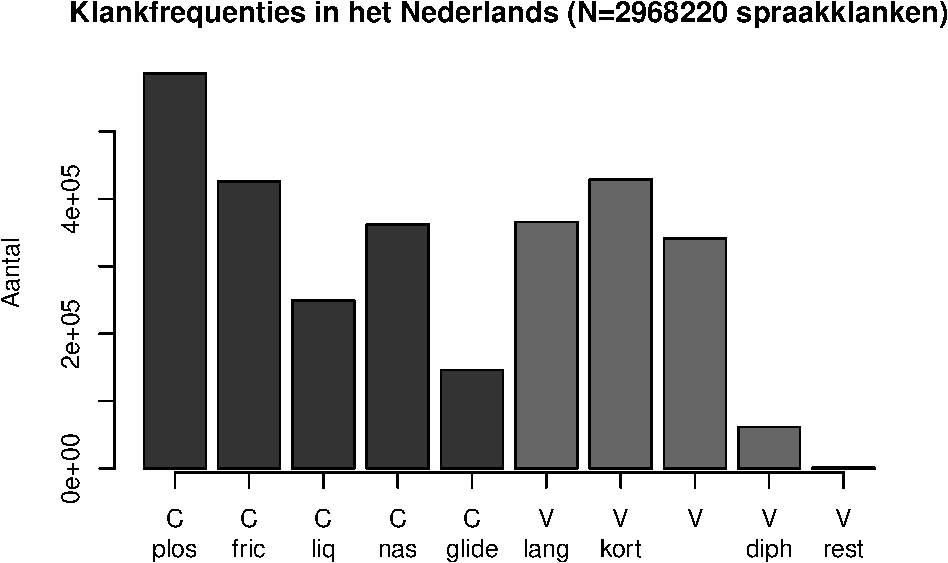
\includegraphics{KMS-NL_files/figure-latex/klankfreq-barplot-1.pdf}
\caption{\label{fig:klankfreq-barplot}Staafdiagram van de frequentieverdeling van fonologische klasse van spraakklanken in het Corpus Gesproken Nederlands (C=consonant=medeklinker, V=vocaal=klinker).}
\end{figure}

Een staafdiagram helpt ons om in één oogopslag de belangrijkste
kenmerken te bepalen van de verdeling van een discrete variabele: de
meest kenmerkende (meest voorkomende) waarde, en de spreiding over
categorieën. Voor de klankfrequenties in het Nederlands
(Figuur \ref{fig:klankfreq-barplot}) zien we dat bij de medeklinkers de
plosieven het meeste voorkomen, dat bij de klinkers de korte klinkers
het meeste voorkomen, dat tweeklanken weinig gebruikt worden (zgn.
diphthongs, de klinkers in \emph{ei, ui, au}), en dat er meer medeklinkers
dan klinkers gesproken worden.

Tip: Vermijd schaduwen en andere 3D-effecten in een staafdiagram! De
breedte en hoogte van een rechthoek wordt daardoor minder goed leesbaar,
en de zichtbare oppervlakte van een beschaduwde rechthoek of van een
balk correspondeert niet meer goed met de frequentie.

\hypertarget{sec:histogrammen}{%
\section{Histogrammen}\label{sec:histogrammen}}

Een histogram is de grafische weergave van een frequentieverdeling van
een continue, numerieke variabele (van interval- of ratio-meetniveau).
Een histogram is opgebouwd uit rechthoeken. De breedte van elke
rechthoek correspondeert met de intervalbreedte (een rechthoek kan ook 1
eenheid breed zijn) en de hoogte correspondeert met de frequentie van
dat interval of van die waarde. De oppervlakte van iedere rechthoek
correspondeert dus met de frequentie. In tegenstelling tot een
staafdiagram sluiten de rechthoeken op elkaar aan langs de horizontale
as.

\begin{figure}
\centering
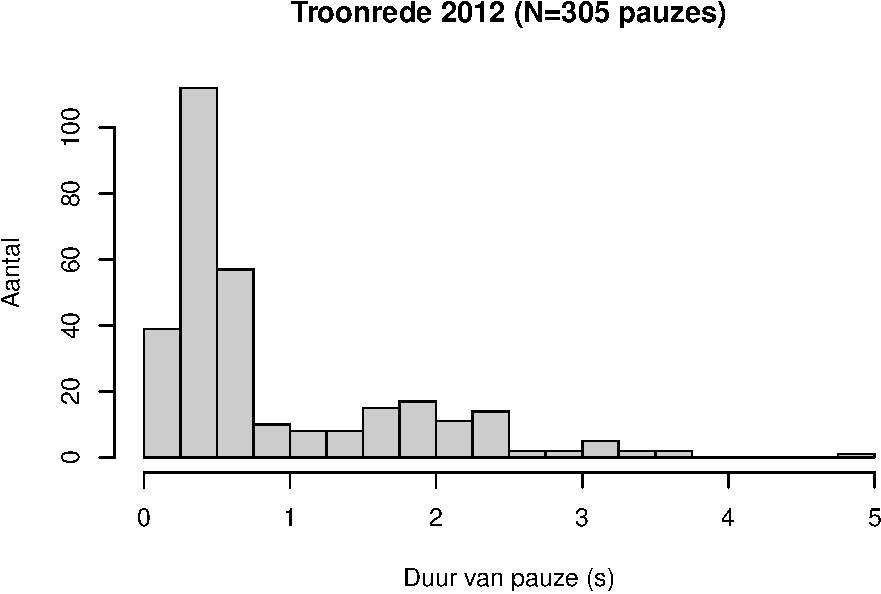
\includegraphics{KMS-NL_files/figure-latex/troonrede2012-hist-1.pdf}
\caption{\label{fig:troonrede2012-hist}Histogram van de duren van spreekpauzes (in seconden) in de Troonrede van 18 september 2012, voorgelezen door Koningin Beatrix (N=305).}
\end{figure}

Een histogram helpt ons om in één oogopslag de belangrijkste kenmerken
te bepalen van de verdeling van een continue variabele: de meest
kenmerkende (meest voorkomende) waarde, de mate van spreiding, het
aantal pieken in de frequentieverdeling, de ligging van die pieken, en
eventuele uitbijters
(zie §\ref{sec:uitbijters}).
Voor de pauzes in de Troonrede van 2012
(Figuur \ref{fig:troonrede2012-hist}) zien we dat de meeste pauzes
tussen 0.25 en 0.75 s duren (vermoedelijk zijn dat adempauzes), dat er
twee pieken zijn in de verdeling (de tweede piek ligt bij 2 s),
en dat er één extreem lange pauze is (met een duur van bijna 5 s).

Tip: Vermijd schaduwen en andere 3D-effecten in een histogram! De
breedte en hoogte van een rechthoek wordt daardoor minder goed leesbaar,
en de zichtbare oppervlakte van een beschaduwde rechthoek of van een
balk correspondeert niet meer goed met de frequentie.

\hypertarget{spss-2}{%
\subsection{SPSS}\label{spss-2}}

\begin{verbatim}
Analyze > Descriptive Statistics > Frequencies...
\end{verbatim}

Selecteer variabele (sleep naar paneel ``Variable(s)'').\\
Kies \texttt{Charts}, kies daarna \texttt{Chart\ type:\ Bar\ chart} voor een
staafdiagram of \texttt{Chart\ type:\ Histogram} voor een histogram (zie
bovenstaande tekst voor het verschil tussen deze opties).\\
Bevestig met \texttt{OK}.\\

\hypertarget{r-2}{%
\subsection{R}\label{r-2}}

Een staafdiagram zoals Figuur \ref{fig:klankfreq-barplot} maak je in R met de volgende commando's:

\begin{Shaded}
\begin{Highlighting}[]
\CommentTok{\# lees data}
\NormalTok{klankfreq \textless{}{-}}\StringTok{ }\KeywordTok{read.table}\NormalTok{( }\DataTypeTok{file=}\StringTok{"data/klankfreq.txt"}\NormalTok{, }\DataTypeTok{header=}\NormalTok{T )}
\CommentTok{\# maak barplot van kolom \textasciigrave{}aantal\textasciigrave{} in dataset \textasciigrave{}klankfreq\textasciigrave{}}
\KeywordTok{with}\NormalTok{( klankfreq, }\KeywordTok{barplot}\NormalTok{( aantal, }\DataTypeTok{beside=}\NormalTok{T, }
                          \DataTypeTok{ylab=}\StringTok{"Aantal"}\NormalTok{,}
                          \DataTypeTok{main=}\StringTok{"Klankfrequenties in het Nederlands (N=2968220)"}\NormalTok{,}
                          \DataTypeTok{col=}\KeywordTok{ifelse}\NormalTok{(klankfreq[,}\DecValTok{1}\NormalTok{]}\OperatorTok{==}\StringTok{"V"}\NormalTok{,}\StringTok{"grey40"}\NormalTok{,}\StringTok{"grey20"}\NormalTok{) ) ) {-}\textgreater{}}\StringTok{ }\NormalTok{klankfreq\_barplot}
\CommentTok{\# maak labels langs onderste horizontale as}
\KeywordTok{axis}\NormalTok{(}\DataTypeTok{side=}\DecValTok{1}\NormalTok{, }\DataTypeTok{at=}\NormalTok{klankfreq\_barplot, }\DataTypeTok{labels=}\NormalTok{klankfreq}\OperatorTok{$}\NormalTok{hoofdklasse)}
\KeywordTok{axis}\NormalTok{(}\DataTypeTok{side=}\DecValTok{1}\NormalTok{, }\DataTypeTok{at=}\NormalTok{klankfreq\_barplot, }\DataTypeTok{tick=}\NormalTok{F, }\DataTypeTok{line=}\DecValTok{1}\NormalTok{, }\DataTypeTok{labels=}\NormalTok{klankfreq}\OperatorTok{$}\NormalTok{onderklasse )}
\CommentTok{\# of eenvoudiger: with(klankfreq, barplot(aantal) ) \# alle defaults }
\end{Highlighting}
\end{Shaded}

Een histogram zoals in Figuur \ref{fig:troonrede2012-hist}
maak je in R met de volgende commando's:

\begin{Shaded}
\begin{Highlighting}[]
\CommentTok{\# lees dataset }
\KeywordTok{load}\NormalTok{(}\DataTypeTok{file=}\StringTok{"data/pauses6.Rda"}\NormalTok{)}
\CommentTok{\# haal daaruit pauzeduren (kolom 12) voor jaar 2012, in aparte variabele \textasciigrave{}troon2012\textasciigrave{}}
\NormalTok{troon2012 \textless{}{-}}\StringTok{ }\NormalTok{pauses6[ pauses6}\OperatorTok{$}\NormalTok{jaar}\OperatorTok{==}\DecValTok{2012}\NormalTok{, }\DecValTok{12}\NormalTok{ ] }\CommentTok{\# save col\_12 as single vector}
\CommentTok{\# maak histogram}
\KeywordTok{hist}\NormalTok{( troon2012, }
      \DataTypeTok{breaks=}\KeywordTok{seq}\NormalTok{(}\DecValTok{0}\NormalTok{, }\DecValTok{5}\NormalTok{, }\DataTypeTok{by=}\FloatTok{0.25}\NormalTok{),}
      \DataTypeTok{col=}\StringTok{"grey80"}\NormalTok{,}
      \DataTypeTok{xlab=}\StringTok{"Duur van pauze (s)"}\NormalTok{, }\DataTypeTok{ylab=}\StringTok{"Aantal"}\NormalTok{, }
      \DataTypeTok{main=}\StringTok{"Troonrede 2012 (N=305 pauzes)"}\NormalTok{ ) {-}\textgreater{}}\StringTok{ }\NormalTok{troonrede2012pauzes\_hist}
\end{Highlighting}
\end{Shaded}

\hypertarget{ch:centrumenspreiding}{%
\chapter{Centrum en spreiding}\label{ch:centrumenspreiding}}

\hypertarget{inleiding-4}{%
\section{Inleiding}\label{inleiding-4}}

In het vorige hoofdstuk hebben we geleerd om observaties te tellen en te
classificeren. Daarmee kunnen we de observaties van een variabele
samenvatten, bijvoorbeeld in een tabel, een frequentieverdeling, of in
een histogram. Vaak kunnen we de observaties nog verder samenvatten, in
kenmerken die aangeven op welke wijze de observaties verdeeld zijn. In
dit hoofdstuk maken we kennis met een aantal van dergelijke kenmerken.
Sommige van die kenmerken zijn van toepassing op variabelen van alle
meetniveau's (bv. modus), andere alleen op variabelen van interval- of
ratio-niveau (bv. gemiddelde). Na een inleiding over het gebruik van
symbolen bespreken we eerst hoe we het centrum van een verdeling kunnen
beschrijven, en hoe we de spreiding kunnen beschrijven.

\hypertarget{symbolen}{%
\section{Symbolen}\label{symbolen}}

In de beschrijvende statistiek wordt veel gewerkt met symbolen. Die
symbolen zijn verkorte aanduidingen voor een reeks van handelingen.
Sommige van die symbolen zijn je reeds bekend: de exponent \({}^2\) in de
uitdrukking \(x^2\) is een symbool met de betekenis ``vermenigvuldig \(x\)
met zichzelf'', ofwel \(x^2 = x \times x\) (waarin ook \(\times\) weer een
symbool is).

Vaak wordt een hoofdletter gebruikt om een variabele aan te duiden
(\(X\)), en een kleine letter om een afzonderlijke score van die variabele
aan te duiden (\(x\)). Als we de afzonderlijke scores willen
onderscheiden, dan doen we dat met een subscript index: \(x_1\) is de
eerste observatie, \(x_2\) is de tweede observatie, enz. Op deze manier
geeft \(x_i\) de \(i\)'de score aan, of de score van proefpersoon nummer
\(i\), van variabele \(X\). Als we willen generaliseren over alle scores,
dan kunnen we de index weglaten, maar we kunnen ook een punt gebruiken
als ``lege'' index: in de uitdrukking \(x_.\) staat de punt-index voor
iedere willekeurige index.

Het aantal observaties in een bepaalde groep geven we aan met kleine
letter \(n\), en het totaal aantal observaties van een variabele met de
hoofdletter \(N\). Als er maar één groep is, zoals in de voorbeelden in
dit hoofdstuk, dan geldt dat \(n=N\).

In de beschrijvende statistiek wordt veel opgeteld, en daarvoor is dan
ook een apart symbool, \(\sum\), de griekse hoofdletter Sigma, waarmee een
sommering of optelling wordt aangeduid. We zouden kunnen zeggen ``tel
alle geobserveerde waarden van variabele \(X\) bij elkaar op'', maar dat
doen we doorgaans korter:
\[\sum\limits_{i=1}^n x_i, \textrm{of korter} \sum x
%   \Sigma_i^N x_i, \textrm{of nog korter} \Sigma X
\]
Op deze wijze
wordt aangegeven dat alle scores \(x_i\) bij elkaar moeten worden opgeteld
(gesommeerd), voor alle waarden van \(i\) (vanaf \(i=1\), tenzij anders
aangegeven) tot \(i=n\). Alle \(n\) scores van de variabele \(x\) moeten dus
worden opgeteld.

Als er haakjes gebruikt worden, let dan goed op: handelingen beschreven
binnen een paar haakjes hebben voorrang, die moet je dus eerst
uitvoeren. Ook als dat niet strikt nodig is, zullen we vaak haakjes
gebruiken ter verduidelijking, zoals in \((2\times3)+4=10\).

\hypertarget{centrummaten}{%
\section{Centrummaten}\label{centrummaten}}

\hypertarget{sec:gemiddelde}{%
\subsection{gemiddelde}\label{sec:gemiddelde}}

De meest bekende maat voor het centrum van een verdeling is wel het
gemiddelde. Het gemiddelde is eenvoudig uit te rekenen door alle scores
bij elkaar op te tellen, en vervolgens die som weer te delen door het
aantal observaties. In symbolen:
\begin{equation} 
  \overline{x} = \frac{\sum x}{n} = \frac{1}{n} \sum\limits_{i}^n x_i
  \label{eq:gemiddelde}
\end{equation}

We maken hier meteen kennis met een nieuw symbool, \(\overline{x}\), vaak
``x-bar'' genoemd, waarmee het gemiddelde van \(x\) wordt aangeduid. Het gemiddelde
wordt ook vaak aangeduid met het symbool \(M\) (Eng. mean), o.a. in
artikelen in de APA-stijl.

\begin{center}\rule{0.5\linewidth}{0.5pt}\end{center}

\begin{quote}
\emph{Voorbeeld 9.1}: In
een winkel wordt bijgehouden hoe lang klanten moeten wachten bij de
kassa, voordat ze aan de beurt zijn. Voor \(N=10\) klanten worden de
volgende wachttijden geobserveerd, in minuten:\\
1, 2, 5, 2, 2, 2, 3, 1, 1, 3.\\
De gemiddelde wachttijd is \((\sum X)/N = 22/10 = 2.2\) minuten.
\end{quote}

\begin{center}\rule{0.5\linewidth}{0.5pt}\end{center}

Het gemiddelde van \(X\) wordt meestal uitgedrukt met één decimaalcijfer meer dan
de scores van \(X\) (zie ook §\ref{sec:significantecijfers-gemiddelde} hieronder over het aantal decimaalcijfers waarmee het gemiddelde wordt weergegeven).

Het gemiddelde is op te vatten als het ``balanspunt'' van een verdeling:
de observaties aan weerszijden houden elkaar ``in evenwicht'', zoals
geïllustreerd in Figuur \ref{fig:wachttijden-hist}, waar de ``blokken'' van het histogram
precies ``in evenwicht'' zijn op het ``balanspunt'' bij het gemiddelde van
2.2. Het gemiddelde is ook de waarde ten opzichte waarvan de \(N\)
observaties tezamen het minste verschillen, en het vormt dus een goed
kenmerk voor het centrum van een kansverdeling.

Het gemiddelde is alleen bruikbaar bij variabelen van het interval- of
ratio-meetniveau.

\begin{figure}
\centering
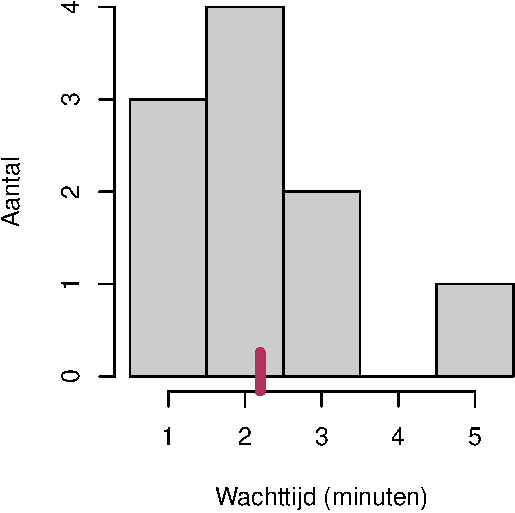
\includegraphics{KMS-NL_files/figure-latex/wachttijden-hist-1.pdf}
\caption{\label{fig:wachttijden-hist}Histogram van N=10 wachttijden, met markering van het gemiddelde.}
\end{figure}

\hypertarget{sec:mediaan}{%
\subsection{mediaan}\label{sec:mediaan}}

De mediaan (symbool \(Md\) of \(\tilde{x}\)) is de observatie in het midden
van de rangorde van observaties \footnote{In het Engels wordt de streep in het midden van een weg aangeduid als de ``median''; deze streep verdeelt de weg in twee even brede helften.}. Als we de scores van \(X\)
rangschikken van klein naar groot, dan is de mediaan het middenpunt van
die gerangschikte reeks. De helft van de observaties is kleiner dan de
mediaan, en de andere helft is groter dan de mediaan.

Bij een oneven aantal observaties is de middelste observatie de mediaan.
Bij een even aantal observaties wordt de mediaan gevormd door het
gemiddelde van de middelste twee observaties.

\begin{center}\rule{0.5\linewidth}{0.5pt}\end{center}

\begin{quote}
\emph{Voorbeeld 9.2}: De wachttijden uit Voorbeeld 9.1
worden als volgt gerangschikt:\\
1, 1, 1, 2, \emph{2, 2}, 2, 3, 3, 5.\\
De mediaan is het gemiddelde van de middelste twee (cursieve)
observaties, dus 2 minuten.
\end{quote}

\begin{center}\rule{0.5\linewidth}{0.5pt}\end{center}

De mediaan is minder gevoelig dan het gemiddelde voor extreme waarden
van \(x\). In het bovenstaande voorbeeld is de extreme wachttijd van 5
minuten van aanzienlijke invloed op het gemiddelde. Als we die waarde
zouden verwijderen, dan verandert het gemiddelde van 2.2 naar 1.9, maar
de mediaan blijft nog steeds 2. Extreme waarden hebben dus een minder
grote invloed op de mediaan dan op het gemiddelde. Pas als de
rangschikking van de observaties verandert, kan ook de mediaan
veranderen.

De mediaan is bruikbaar bij variabelen van het ordinale, interval- of
ratio-meetniveau.

\hypertarget{modus}{%
\subsection{modus}\label{modus}}

De modus (bijv.nw. `modaal') is de waarde of score van \(X\) die het
meeste voorkomt.

\begin{center}\rule{0.5\linewidth}{0.5pt}\end{center}

\begin{quote}
\emph{Voorbeeld 9.3}: Bij de wachttijden uit Voorbeeld 9.1
komt de score 2 het meeste voor
(\(4\times\)); dit is de modus.
\end{quote}

\begin{center}\rule{0.5\linewidth}{0.5pt}\end{center}

\begin{quote}
\emph{Voorbeeld 9.4}: In 2014 was het gemiddelde inkomen per huishouden in Nederland €34200.
Het modale inkomen (per huishouden) lag tussen €18000 en €20000\footnote{\url{http://www.cbs.nl/nl-NL/menu/themas/inkomen-bestedingen/cijfers/extra/inkomensverdeling.htm}}. In
2014 vielen de meeste huishoudens in Nederland dus in deze inkomens-klasse.
\end{quote}

\begin{center}\rule{0.5\linewidth}{0.5pt}\end{center}

De modus is nog minder gevoelig dan de mediaan voor extreme waarden van
\(x\). In het bovenstaande voorbeeld 9.2 maakt het niet uit wat de waarde
van de langste wachttijd is: ook al zou die observatie de waarde \(10\) of
\(1000\) hebben, de modus blijft onveranderlijk \(2\) (ga dat zelf na).

De modus is bruikbaar bij variabelen van alle meetniveau's.

\hypertarget{sec:harmonischgemiddelde}{%
\subsection{harmonisch gemiddelde}\label{sec:harmonischgemiddelde}}

Als de afhankelijke variabele een breuk of verhouding of ratio
voorstelt, zoals de snelheid waarmee een taak verricht wordt, dan vormt
het (rekenkundig) gemiddelde van formule \eqref{eq:gemiddelde}
eigenlijk niet een goede aanduiding voor de
meest kenmerkende of centrale waarde. In dat geval kan je beter het
harmonisch gemiddelde gebruiken:

\begin{equation}
  H = \frac{1}{\frac{1}{n} \sum\limits_{i}^n \frac{1}{x_i} } = \frac{n}{\sum\limits_{i}^n \frac{1}{x_i}}
  \label{eq:harmonischgemiddelde}
\end{equation}

\begin{center}\rule{0.5\linewidth}{0.5pt}\end{center}

\begin{quote}
\emph{Voorbeeld 9.5}:
Een student schrijft \(n=3\) teksten. Over de eerste tekst (500 woorden)
doet hij 2.5 uur, over de tweede tekst (1000 woorden) doet hij 4 uur, en
over de derde tekst (300 woorden) doet hij 0.6 uur. Wat is de gemiddelde
schrijfsnelheid van deze student? De schrijfsnelheden zijn resp. 200,
250, en 500 woorden per uur, en het ``normale'' (rekenkundig) gemiddelde
daarvan is 317 woorden per uur. Het ``eigenlijke'' gemiddelde is
echter \((500+1000+300)/(2.5+4+0.6)\) \(=1800/7.1=254\) woorden per uur. De hoge
schrijfsnelheid van de korte tekst telt voor \(1/n\) deel mee in het
rekenkundig gemiddelde, hoewel die tekst slechts \(300/1800=1/6\) van het
totaal aantal woorden bevat.
\end{quote}

\begin{quote}
Omdat de afhankelijke variabele een breuk is (snelheid, woorden/uur),
vormt het harmonische gemiddelde hier een betere centrummaat. Eerst
rekenen we de snelheid (woorden per tijdseenheid) om naar de inverse
daarvan (zie \eqref{eq:harmonischgemiddelde}, in noemer, binnen somteken),
d.w.z. naar \emph{tijd} per woord: 0.005, 0.004, en 0.002 (tijdseenheden per
woord, zie voetnoot\footnote{Dit is vergelijkbaar met sporten als roeien, zwemmen, wielrennen, schaatsen, e.d., waar ook de tijd over een afgesproken afstand gemeten en vergeleken wordt, en niet de snelheid over een afgesproken tijd.}). Ten tweede middelen we deze tijden, tot
gemiddeld 0.00366 uur per woord, en tenslotte nemen we daarvan wederom
de inverse. De harmonisch gemiddelde schrijfsnelheid is dan \(1/0.00366=273\)
woorden per uur, dichter bij het ``eigenlijke'' gemiddelde van 254 woorden
per uur.
\end{quote}

\begin{center}\rule{0.5\linewidth}{0.5pt}\end{center}

\hypertarget{gewinsoriseerde-gemiddelde}{%
\subsection{gewinsoriseerde gemiddelde}\label{gewinsoriseerde-gemiddelde}}

De grote gevoeligheid van het gewone (rekenkundige) gemiddelde voor
uitbijters kan ingeperkt worden, door de meest extreme observaties te
wijzigen naar de minder extreme, meer centrale observaties. Het
gemiddelde van deze (deels gewijzigde) observaties wordt het
\emph{gewinsoriseerde} gemiddelde genoemd (``winsorized mean''; ).

\begin{center}\rule{0.5\linewidth}{0.5pt}\end{center}

\begin{quote}
\emph{Voorbeeld 9.6}: De wachttijden uit Voorbeeld 9.1
worden als volgt gerangschikt:\\
1, 1, 1, 2, 2, 2, 2, 3, 3, 5.\\
Voor het 10\% gewinsoriseerde gemiddelde worden (na rangordening) de 10\%
kleinste observaties gelijk gesteld aan de eerstvolgende grotere waarde,
en de 10\% grootste observaties worden gelijk gesteld aan de laatst
voorafgaande kleinere waarde (gewijzigde waarden zijn hier cursief):\\
\emph{1}, 1, 1, 2, 2, 2, 2, 3, 3, \emph{3}.\\
Het winsorized gemiddelde over deze gewijzigde waarden is
\(\overline{x}_w=2\) minuten.
\end{quote}

\begin{center}\rule{0.5\linewidth}{0.5pt}\end{center}

\hypertarget{getrimde-gemiddelde}{%
\subsection{getrimde gemiddelde}\label{getrimde-gemiddelde}}

Een nog drastischer ingreep is om de meest extreme observaties geheel te
verwijderen. Het gemiddelde van de overblijvende observaties wordt het
\emph{getrimde} gemiddelde genoemd (``trimmed mean''). Bij een 10\% trim
verwijderen we de onderste 10\% \emph{en} de bovenste 10\% van de observaties;
er resteren dan dus nog slechts \((1- (2 \times (10/100))\times n\)
observaties \citep{Wilcox12}.

\begin{center}\rule{0.5\linewidth}{0.5pt}\end{center}

\begin{quote}
\emph{Voorbeeld 9.7}: De wachttijden uit Voorbeeld 9.1
worden weer als volgt gerangschikt:\\
1, 1, 1, 2, 2, 2, 2, 3, 3, 5.\\
Voor het 10\% getrimde gemiddelde worden (na rangordening) de 10\%
kleinste observaties verwijderd, en de 10\% grootste observaties worden
eveneens verwijderd:\\
1, 1, 2, 2, 2, 2, 3, 3.\\
Het getrimde gemiddelde over deze \(10-(.2)(10)=8\) resterende waarden is
hier \(\overline{x}_t=2\) minuten.
\end{quote}

\begin{center}\rule{0.5\linewidth}{0.5pt}\end{center}

\hypertarget{vergelijking-van-centrummaten}{%
\subsection{vergelijking van centrummaten}\label{vergelijking-van-centrummaten}}

Figuur \ref{fig:centrummaten} illustreert de verschillen tussen de
diverse centrummaten, voor asymmetrisch verdeelde observaties.

\begin{figure}
\centering
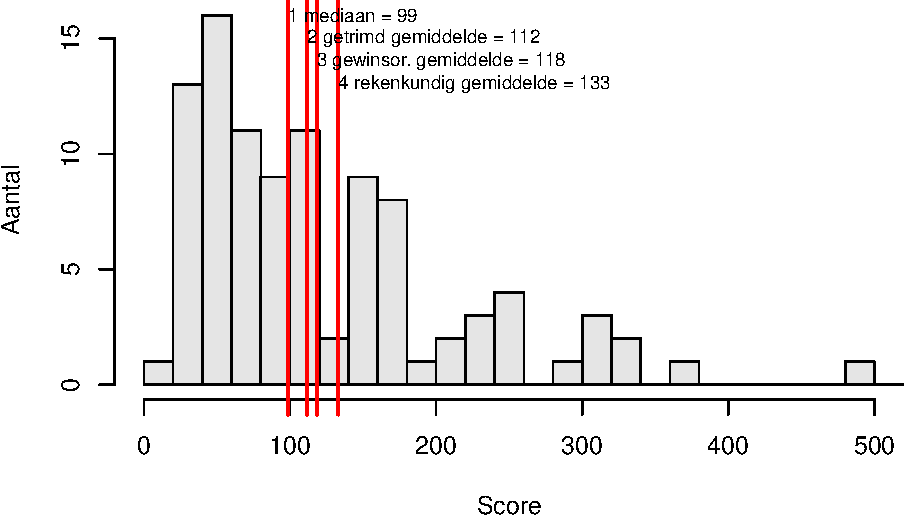
\includegraphics{KMS-NL_files/figure-latex/centrummaten-1.pdf}
\caption{\label{fig:centrummaten}Histogram van een variabele met positief scheve (asymmetrische) frequentieverdeling, met daarin aangegeven (1) de mediaan, (2) het 10\% getrimde gemiddelde, (3) het 10\% gewinsoriseerde gemiddelde, en (4) het rekenkundig gemiddelde. De geobserveerde scores zijn gemarkeerd langs de horizontale as.}
\end{figure}

Het rekenkundig gemiddelde is het meest gevoelig voor extreme waarden:
de extreme waarden ``trekken'' erg hard aan het gemiddelde. Deze invloed
van extreme waarden wordt getemperd in het gewinsoriseerde gemiddelde,
en wordt nog meer getemperd in het getrimde gemiddelde. Naarmate de
trimfactor (het percentage van de observaties dat wordt gewijzigd of
verwijderd) toeneemt, gaan de gewinsoriseerde en getrimde gemiddelden
meer lijken op de mediaan. Immers, bij een trimfactor van 50\% resteert
er van alle observaties nog maar één (ongewijzigde) observatie, en dat
is de mediaan (ga dat zelf na). In
§\ref{sec:robuustefficient} gaan we verder in op de keuze voor een
passende maat voor het centrum van een verdeling.

\hypertarget{sec:kwartielen-en-boxplots}{%
\section{Kwartielen en boxplots}\label{sec:kwartielen-en-boxplots}}

De verdeling van een variabele wordt niet alleen gekenmerkt door het
centrum van die verdeling, maar ook door de mate van spreiding rondom
het centrum, d.w.z. hoe groot het verschil is van de observaties t.o.v.
het gemiddelde. We willen bijvoorbeeld niet alleen weten wat het
gemiddelde inkomen is, maar ook hoe groot de \emph{verschillen} in inkomen
zijn.

\hypertarget{kwartielen}{%
\subsection{Kwartielen}\label{kwartielen}}

Een eenvoudige en bruikbare maat daarvoor zijn de kwartielen \citep{Tukey77}.
We delen de gerangschikte observaties in twee helften op; de grens
daartussen is de mediaan. Vervolgens halveren we weer elke helft, tot
kwarten. De kwartielen worden gevormd door de grenzen tussen deze
kwarten; er zijn dus drie kwartielen. Het eerste kwartiel \(Q_1\) is de
mediaan van de onderste helft, \(Q_2\) is de mediaan van alle \(n\)
observaties, en het derde kwartiel \(Q_3\) is de mediaan van de bovenste
helft. De helft van de observaties (nl. het tweede en derde kwart) ligt
tussen \(Q_1\) en \(Q_3\). De afstand tussen \(Q_1\) en \(Q_3\) wordt de
``interquartile range'' genoemd (IQR). Deze IQR vormt een eerste bruikbare
maat voor de spreiding van observaties ten opzichte van hun centrale
waarde.

Voor de uitleg maken we gebruik van de fictieve scores op een leestoets,
gegeven in Tabel \ref{tab:cito}.

\begin{longtable}[]{@{}cccc@{}}
\caption{\label{tab:cito} Scores van N=10 leerlingen op drie onderdelen van de CITO-toets,
afgenomen in groep 8 van het basisonderwijs.}\tabularnewline
\toprule
Leerling & Lezen & Rekenen & Wereldoriëntatie\tabularnewline
\midrule
\endfirsthead
\toprule
Leerling & Lezen & Rekenen & Wereldoriëntatie\tabularnewline
\midrule
\endhead
1 & 18 & 22 & 55\tabularnewline
2 & 32 & 36 & 55\tabularnewline
3 & 45 & 34 & 38\tabularnewline
4 & 25 & 25 & 40\tabularnewline
5 & 27 & 29 & 48\tabularnewline
6 & 23 & 20 & 44\tabularnewline
7 & 29 & 27 & 49\tabularnewline
8 & 26 & 25 & 42\tabularnewline
9 & 20 & 25 & 57\tabularnewline
10 & 25 & 27 & 47\tabularnewline
\(\sum x\) & 270 & 270 & 475\tabularnewline
\(\overline{x}\) & 27.0 & 27.0 & 47.5\tabularnewline
\bottomrule
\end{longtable}

\begin{center}\rule{0.5\linewidth}{0.5pt}\end{center}

\begin{quote}
Voorbeeld 9.8:
De scores bij het onderdeel Lezen in
Tabel \ref{tab:cito} zijn
als volgt gerangschikt:\\
18, 20, 23, 25, 25, 26, 27, 29, 32, 45.\\
De mediaan is \(Q_2=25.5\) (tussen de 5e en 6e observatie in deze
ranglijst). De mediaan van de onderste helft is \(Q_1=23\) en die van de
bovenste helft is \(Q_3=29\). De interquartile range is
\(\textrm{IQR}=29-23=6\).
\end{quote}

\begin{center}\rule{0.5\linewidth}{0.5pt}\end{center}

\hypertarget{sec:uitbijters}{%
\subsection{Uitbijters}\label{sec:uitbijters}}

In de leesscores in Tabel \ref{tab:cito} treffen we een extreme waarde aan, nl. de score
45, die opvallend veel verschilt van het gemiddelde. Zo'n opvallende
waarde wordt aangeduid als een ``uitbijter'' (in het Engels als
``outlier''). De grens voor wat we beschouwen als een uitbijter ligt
doorgaans bij \(1.5 \times \textrm{IQR}\). Als een waarde meer dan
\(1.5 \times \textrm{IQR}\) boven \(Q_3\) of onder \(Q_1\) ligt, dan
beschouwen we die observatie als een uitbijter. Controleer deze
observaties nog eens (denk aan het principe van zorgvuldigheid, zie
§\ref{sec:integriteit-inleiding}).

\begin{center}\rule{0.5\linewidth}{0.5pt}\end{center}

\begin{quote}
Voorbeeld 9.9:
Voor de eerder genoemde leesscores in
Tabel \ref{tab:cito} vonden
we \(Q_1=23\), \(Q_3=29\), en \(\textrm{IQR}=Q_3-Q_1=29-23=6\). De bovenste
grenswaarde voor uitbijters is
\(Q_3 + 1.5 \times \textrm{IQR} = 29 + 1.5 \times 6 = 29+9 = 38\). De
observatie met score 45 ligt boven deze grenswaarde, en wordt daarom
beschouwd als uitbijter.
\end{quote}

\begin{center}\rule{0.5\linewidth}{0.5pt}\end{center}

\hypertarget{sec:boxplot}{%
\subsection{Boxplots}\label{sec:boxplot}}

De frequentieverdeling van een variabele kunnen we nu weergeven met vijf
kenmerken, de zgn. ``five-number summary'', nl. de kleinste waarde, \(Q_1\),
mediaan, \(Q_3\), en grootste waarde. Deze vijf kenmerken worden grafisch
weergegeven in een zgn. ``boxplot'', zie
Figuur \ref{fig:cito-boxplot} voor een voorbeeld \citep[ §2C]{Tukey77}.

\begin{figure}
\centering
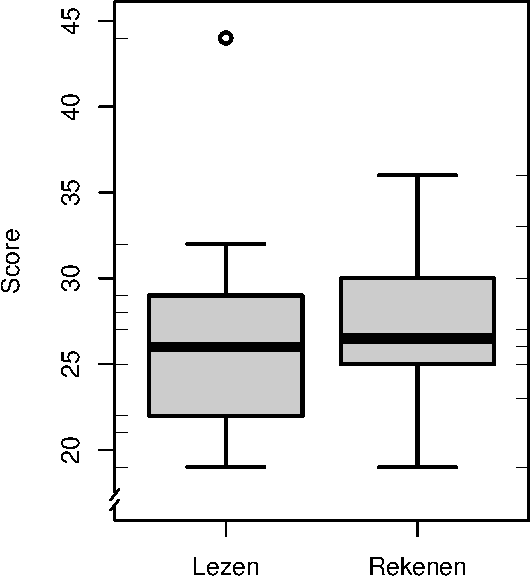
\includegraphics{KMS-NL_files/figure-latex/cito-boxplot-1.pdf}
\caption{\label{fig:cito-boxplot}Boxplots van scores van \(N=10\) leerlingen op de onderdelen Lezen en Rekenen van de CITO-toets (zie Tabel 9.1), met uitbijters als open cirkels gemarkeerd. De geobserveerde scores zijn gemarkeerd langs de verticale assen.}
\end{figure}

De box omspant het gebied van (bij benadering) \(Q_1\) tot \(Q_3\), en
omspant dus de centrale helft van de observaties. De dikkere lijn in de
box markeert de mediaan. De lijnen strekken zich uit naar de kleinste en
grootste waarden \emph{die géén uitbijters zijn} \footnote{In een klassieke boxplot strekken de lijnen zich uit naar het minimum en maximum \citep{Tukey77} en worden uitbijters niet apart aangeduid.}. De afzonderlijke
uitbijters worden hier met een apart symbool aangeduid.

\hypertarget{sec:spreidingsmaten}{%
\section{Spreidingsmaten}\label{sec:spreidingsmaten}}

\hypertarget{sec:variantie}{%
\subsection{variantie}\label{sec:variantie}}

Een andere
manier om de spreiding van de observaties aan te geven, zou zijn om te
kijken naar de afwijking van iedere observatie ten opzichte van het
gemiddelde, dus \((x_i-\overline{x})\). Maar als we al die afwijkingen
optellen, dan is de som daarvan altijd nul! De positieve en negatieve
afwijkingen heffen elkaar immers op (ga dat zelf na in
Tabel @\#ref(tab:cito)).
Daarom middelen we niet de afwijkingen zelf, maar de kwadraten van die
afwijkingen. Zowel de positieve als de negatieve afwijkingen resulteren
in positieve gekwadrateerde-afwijkingen. Van al die
gekwadrateerde-afwijkingen berekenen we het gemiddelde, d.w.z. we tellen
ze op en delen door \((n-1)\), zie voetnoot\footnote{We delen door \(n-1\) en niet door \(n\), om een betere schatting te krijgen van de spreiding in de \emph{populatie}. Op deze manier houden we rekening met het feit dat we één kenmerk van de steekproef (nl. het gemiddelde) gebruiken om de spreiding te bepalen. Als je alleen geïnteresseerd bent in de spreiding in je \emph{steekproef} van observaties, en niet in de populatie, deel dan door \(n\).}. Het resultaat noemen we
de \emph{variantie}, aangeduid met symbool \(s^2\):
\begin{equation}
  s^2 = \frac{ \sum (x_i - \overline{x})^2 } {n-1}
  \label{eq:variantie}
\end{equation}

De teller van
deze breuk wordt wel aangeduid als de ``sum of squared deviations'' of
``sum of squares'' (SS) en de noemer wordt wel aangeduid als het aantal
vrijheidsgraden of ``degrees of freedom'' van de teller (d.f.; zie
§\ref{sec:ttoets-vrijheidsgraden}).

De variantie rekenen we tegenwoordig altijd uit met een rekenmachine of
computer.

\hypertarget{sec:standaarddeviatie}{%
\subsection{standaarddeviatie}\label{sec:standaarddeviatie}}

Om de bovenstaande variantie te berekenen, hebben we de afwijkingen van
de observaties gekwadrateerd. De variantie is dus een grootheid die niet
wordt uitgedrukt in de oorspronkelijke eenheden (bijv. seconden, cm,
score), maar in gekwadrateerde eenheden (bijv. \(\textrm{s}^2\),
\(\textrm{cm}^2\), \(\textrm{score}^2\)). Teneinde weer terug te keren naar
de oorspronkelijke eenheden, nemen we de wortel uit de variantie. Het
resultaat noemen we de \emph{standaarddeviatie}, aangeduid met symbool \(s\):

\begin{equation}
  s = \sqrt{s^2} = \sqrt{ \frac{ \sum (x_i - \overline{x})^2 } {n-1} }
  \label{eq:standaarddeviatie}
\end{equation}

\begin{center}\rule{0.5\linewidth}{0.5pt}\end{center}

\begin{quote}
Voorbeeld 9.10:
Het gemiddelde van de eerder genoemde leesscores in
Tabel \ref{tab:cito} is
\(27.0\), en de afwijkingen zijn als volgt:\\
-9, 5, 18, -2, 0, -4, 2, -1, -7, -2.\\
De gekwadrateerde afwijkingen zijn 81, 25, 324, 4, 0, 16, 4, 1, 49, 4.\\
De som van deze gekwadrateerde afwijkingen is 508, en de variantie is
dan \(s^2=508/9=56.44\). De standaarddeviatie is de wortel van de
variantie, dus \(s=\sqrt{508/9}=7.5\).
\end{quote}

\begin{center}\rule{0.5\linewidth}{0.5pt}\end{center}

De variantie en standaarddeviatie zijn alleen bruikbaar bij variabelen
van het interval- of ratio-meetniveau. Ook de variantie en
standaarddeviatie kunnen weer gebaseerd zijn op de gewinsoriseerde of
getrimde verzameling van observaties.

De standaarddeviatie hebben we nodig
(a) als we de ruwe observaties
willen omzetten naar standaardscores (zie §\ref{sec:standaardscores} hieronder),
(b) als we een variabele
willen beschrijven die normaal verdeeld is (zie §\ref{sec:normaalverdeling}, en
(c) als we hypotheses willen toetsen met behulp van een normaal verdeelde variabele (zie §@ref(sec:ttoets.onesample) e.v.).

\hypertarget{mad}{%
\subsection{MAD}\label{mad}}

Behalve de standaarddeviatie is er ook een robuuste tegenhanger daarvan,
die niet gebruik maakt van het gemiddelde. Deze maat is daarom minder
gevoelig voor uitbijters (robuuster), wat soms handig is.

We kijken hiervoor naar de afwijking van iedere observatie ten opzichte
van de mediaan (niet t.o.v. het gemiddelde). Van deze afwijkingen nemen
we de absolute waarde\footnote{Positieve afwijkingen blijven ongewijzigd, van negatieve afwijkingen wordt het teken omgekeerd.} (niet het kwadraat). Van deze absolute
afwijkingen bepalen we tenslotte weer de mediaan (niet het gemiddelde).
Het resultaat noemen we de ``median absolute deviation'' (MAD):
\begin{equation}
  \textrm{MAD} = k ~~ Md ( |x_i - Md(x) |)
  \label{eq:MAD}
\end{equation}

Hierbij gebruiken we meestal \(k=1.4826\) als constante; door deze schaalfactor komt de MAD
ruwweg overeen met de standaarddeviatie \(s\) indien \(x\) normaal verdeeld
zou zijn (§\ref{sec:normaalverdeling}).

\begin{center}\rule{0.5\linewidth}{0.5pt}\end{center}

\begin{quote}
Voorbeeld 9.11:
De mediaan van de eerder genoemde leesscores in
Tabel \ref{tab:cito} is
25.5, en de afwijkingen van die mediaan zijn als volgt:\\
-7.5, 6.5, 19.5, -0.5, 1.5, -2.5, 3.5, 0.5, -5.5, -0.5.\\
De gerangschikte, absolute afwijkingen zijn\\
0.5, 0.5, 0.5, 1.5, \emph{2.5, 3.5}, 5.5, 6.5, 7.5, 19.5.\\
De mediaan van deze 10 absolute afwijkingen is 3, en
\(\textrm{MAD} = 1.4826 \times 3 = 4.4478\). Merk op dat de MAD kleiner is
dan de standaarddeviatie, o.a. omdat de MAD minder gevoelig is voor de
extreme waarde \(x_3=45\).
\end{quote}

\begin{center}\rule{0.5\linewidth}{0.5pt}\end{center}

\hypertarget{sec:significantecijfers}{%
\section{Over significante cijfers}\label{sec:significantecijfers}}

\hypertarget{sec:significantecijfers-gemiddelde}{%
\subsection{Gemiddelde en standaarddeviatie}\label{sec:significantecijfers-gemiddelde}}

Een gemiddelde uitkomst wordt weergegeven in een beperkt aantal
significante cijfers, d.i. een beperkt aantal cijfers, van links naar
rechts geteld, zonder acht te slaan op het decimaalteken. Het aantal
significante cijfers van een gemiddelde uitkomst moet gelijk zijn aan
het aantal significante cijfers van het \emph{aantal observaties} waarover is
gemiddeld. (Overige cijfers in de gemiddelde uitkomst zijn niet
nauwkeurig bepaald.) De gemiddelde uitkomst moet eerst afgerond worden
tot het gepaste aantal significante cijfers, voordat de uitkomst verder
geïnterpreteerd wordt, zie
Tabel \ref{tab:signifcijfersgemiddelde}.

\begin{longtable}[]{@{}cccc@{}}
\caption{\label{tab:signifcijfersgemiddelde} Het aantal significante cijfers in het gerapporteerde gemiddelde is gelijk aan het aantal significante cijfers van het aantal observaties.}\tabularnewline
\toprule
aant.obs. & aant.signif.cijfers & voorbeeld gemiddelde & rapporteer als\tabularnewline
\midrule
\endfirsthead
\toprule
aant.obs. & aant.signif.cijfers & voorbeeld gemiddelde & rapporteer als\tabularnewline
\midrule
\endhead
\(1\dots9\) & 1 & 21/8 = 2.625 & 3\tabularnewline
\(10\dots99\) & 2 & 57/21 = 2.714286 & 2.7\tabularnewline
\(100\dots999\) & 3 & 317/120 = 2.641667 & 2.64\tabularnewline
\(1000\dots9999\) & 4 & 3179/1234 = 2.576175 & 2.576\tabularnewline
\bottomrule
\end{longtable}

Het aantal significante cijfers in de gerapporteerde standaarddeviatie
is hetzelfde als in het gemiddelde, volgens
Tabel \ref{tab:signifcijfersgemiddelde}.

\hypertarget{achtergrond}{%
\subsubsection{Achtergrond}\label{achtergrond}}

Laten we aannemen dat ik de afstand van mijn huis naar mijn werk langs
een vaste route een aantal keren heb gemeten. Het gemiddelde van die
metingen bedraagt zogenaamd \(2.954321\) km. Door het gemiddelde te
rapporteren met 7 cijfers suggereer ik hier dat ik precies weet dat de
afstand \(2954321\) millimeter is, en ten hoogste \(1\) mm meer of minder:
het laatste cijfer is geschat of afgerond. Het aantal significante
cijfers (in dit voorbeeld 7) geeft de mate van nauwkeurigheid aan. In
dit voorbeeld is de gesuggereerde nauwkeurigheid van 1 mm duidelijk
onjuist, o.a. omdat beginpunt en eindpunt niet tot op de millimeter
bepaald zijn. Het is daarom gebruikelijk om de gemiddelde gemeten
afstand te rapporteren met een aantal significante cijfers dat de
nauwkeurigheid van die metingen en van het gemiddelde aangeeft, bijv.
\(3.0\)~km (per auto of fiets) of \(2.95\)~km (te voet).

Dezelfde gedachtengang is van toepassing bij de meting van een kenmerk
door middel van een enquête-vraag. Met \(n=15\) respondenten zou de
gemiddelde score \(43/15 \approx 2.86667\) kunnen zijn. Maar de
nauwkeurigheid is in dit voorbeeld niet zo goed als dit decimale getal
suggereert. In feite zorgt hier één afwijkend antwoord al voor een
afwijking van \(\pm0.06667\) in het gemiddelde. Bovendien is een
gemiddelde score altijd het resultaat van een deling, en ``(bij) delen
en vermenigvuldigen geldt de regel dat de uitkomst evenveel significante
cijfers bevat als de meetwaarde met het kleinste aantal significante
cijfers.''\footnote{\url{https://nl.wikipedia.org/wiki/Significant_cijfer}} In dit voorbeeld bestaan de teller (\(43\)) en de noemer
(\(15\)) van het gemiddelde beide uit 2 significante cijfers, en dient de
uitkomst dus ook uit 2 significante cijfers te bestaan. De gemiddelde
score dient gerapporteerd te worden als \(2.9\) punten, met slechts één
cijfer achter het decimaalteken.

\hypertarget{percentages}{%
\subsection{Percentages}\label{percentages}}

Een percentage is een verhouding of breuk, vermenigvuldigd met \(100\).
Gebruik en rapporteer een afgerond percentage (d.i. twee significante
cijfers) alleen indien de noemer van de verhouding of breuk groter is
dan 100. Deze noemer geeft het aantal waarnemingen of gevallen. Als de
noemer kleiner is dan 100 (waarnemingen, gevallen), dan zijn percentages
misleidend, zie Tabel \ref{tab:signifcijferspercentage}.

\begin{longtable}[]{@{}cccc@{}}
\caption{\label{tab:signifcijferspercentage} Het aantal significante cijfers in de gerapporteerde proportie (of percentage) hangt samen met het aantal significante cijfers van het aantal observaties in de noemer van de breuk.}\tabularnewline
\toprule
aant.obs.(noemer) & aant.signif.cijfers & voorbeeld breuk & rapporteer als\tabularnewline
\midrule
\endfirsthead
\toprule
aant.obs.(noemer) & aant.signif.cijfers & voorbeeld breuk & rapporteer als\tabularnewline
\midrule
\endhead
\(1\dots9\) & 1 & 3/8 = 0.4 & 3/8\tabularnewline
\(10\dots99\) & 2 & 21/57 = 0.36 & 21/57\tabularnewline
\(100\dots999\) & 3 & 120/317 = 0.378 & 38\%\tabularnewline
\(1000\dots9999\) & 4 & 1234/3179 = 0.3882 & 38.8\%\tabularnewline
\bottomrule
\end{longtable}

\hypertarget{achtergrond-1}{%
\subsubsection{Achtergrond}\label{achtergrond-1}}

De regels voor percentages vloeien voort uit die in
§\ref{sec:significantecijfers-gemiddelde} toegepast op delingen.
Als de noemer groter is dan 100 is het percentage (met twee significante
cijfers) het gevolg van een schaalverandering ``naar beneden'' (van een
noemer groter dan 100 naar een noemer van precies 100 percentagepunten).
De percentageschaal is minder nauwkeurig dan de oorspronkelijke
verhouding; de percentages zijn afgerond tot op twee significante
cijfers; het laatste significante cijfer van het percentage is dus
geborgd.

Als de noemer echter kleiner is dan 100 dan is het percentage (met twee
significante cijfers) het gevolg van een ``oprekking naar boven'' (van een
noemer kleiner dan 100 naar een noemer van precies 100
percentagepunten). De percentageschaal suggereert dan een
pseudo-nauwkeurigheid die er niet was in de oorspronkelijke verhouding,
en de nauwkeurigheid van de percentageschaal is vals. Als de noemer
kleiner is dan 100, zijn percentages dus misleidend.

\begin{center}\rule{0.5\linewidth}{0.5pt}\end{center}

\begin{quote}
Voorbeeld 9.12:
In een cursus van 29 studenten zijn er 23 studenten geslaagd. We spreken
dan vaak van een cursusrendement van \(23/29=\) 79\%. Toch is zo'n weergave
als percentage in dit geval misleidend. Laten we daarvoor eens kijken
naar de 6 gezakten. Je kunt beredeneren dat het aantal van 6 gezakten
een eigen afrondingsfout heeft van \(1/2\) student; bij omzetting naar de
percentageschaal wordt ook deze afrondingsfout mee vergroot, zodat de
percentages minder nauwkeurig zijn dan de hele percentages (2
significante cijfers) suggereren. Of anders gezegd: het aantal van 6
gezakten (d.i. een getal met één significant cijfer) noopt ons om ook de
verhouding weer te geven met slechts één significant cijfer, en dus niet
als percentage. Rapporteer bij voorkeur de verhouding zelf (\(23/29\)), of
eventueel de ``odds'' (\(23/6=4\)) afgerond tot het juiste aantal
significante cijfers\footnote{Deze ``odds'' geeft aan dat er 23 geslaagden zijn op 6 gezakten, d.i. afgerond 4 geslaagden voor iedere gezakte.}.
\end{quote}

\begin{center}\rule{0.5\linewidth}{0.5pt}\end{center}

Op grond van dezelfde overwegingen is een percentage met een decimaal
cijfer (d.i. met drie significante cijfers, bv. ``36.1\%'') alleen zinnig
als de noemer van de verhouding of breuk groter is dan 1000.

\begin{center}\rule{0.5\linewidth}{0.5pt}\end{center}

\begin{quote}
Voorbeeld 9.13:
In 2013 startten 154 studenten met een tweejarige research master. Na 2
jaar waren 69 daarvan afgestudeerd. Het nominaal rendement voor dit
cohort is dan \(69/154=\) 0.448052, af te ronden en te rapporteren als 44\%
(niet als 44.81\%).
\end{quote}

\begin{center}\rule{0.5\linewidth}{0.5pt}\end{center}

\hypertarget{sec:robuustefficient}{%
\section{Keuzemoment}\label{sec:robuustefficient}}

De verdeling van een variabele kun je op verschillende manieren
beschrijven.
Als variabele \(X\) gemeten is op het interval- of ratio-meetniveau,
begin dan altijd met een histogram (§\ref{sec:histogrammen})
en een boxplot (§\ref{sec:boxplot}).

De centrummaten en spreidingsmaten zijn te ordenen zoals in
Tabel \ref{tab:centrumspreidingsmaten}.

\begin{longtable}[]{@{}lll@{}}
\caption{\label{tab:centrumspreidingsmaten} Overzicht van besproken centrummaten en spreidingsmaten.}\tabularnewline
\toprule
Verdeling & Centrummaat & Spreidingsmaat\tabularnewline
\midrule
\endfirsthead
\toprule
Verdeling & Centrummaat & Spreidingsmaat\tabularnewline
\midrule
\endhead
alle & mediaan & kwartielen, IQR, MAD\tabularnewline
\ldots{} & getrimde of gewins.gemidd. & getrimde of gewins.std.dev.\tabularnewline
(a \& b \& c) & gemiddelde & standaarddeviatie\tabularnewline
\bottomrule
\end{longtable}

De meest \textbf{robuuste} maten staan
bovenin (mediaan, kwartielen, IQR, MAD). Deze maten zijn robuust: ze
zijn weinig gevoelig voor uitbijters of voor eventuele \emph{a}symmetrie in de
frequentieverdeling, zoals de voorbeelden in dit hoofdstuk laten zien.

De meest \textbf{efficiënte} maten staan onderin in
Tabel \ref{tab:centrumspreidingsmaten}: gemiddelde en standaarddeviatie.
Deze maten zijn efficiënt: ze geven het centrum en de spreiding het
beste weer, ze hebben zelf de kleinste standaarddeviatie, en ze hebben
daarvoor relatief het kleinste aantal observaties nodig. De andere maten
nemen een tussenpositie in: de getrimde maten zijn wat robuuster, en de
gewinsoriseerde maten wat efficiënter.

De meest efficiënte maten vereisen echter ook de meest vèrgaande
assumpties (en de meest robuuste maten vereisen de minste assumpties).
Deze efficiënte maten zijn alleen zinnig, indien de verdeling van \(X\)
voldoet aan drie assumpties: (a) de verdeling is min of meer
symmetrisch, d.w.z. de linker- en rechter-helft van het histogram resp.
de bovenste en onderste helft van de boxplot lijken elkaars
spiegelbeeld, (b) de verdeling is unimodaal, d.w.z. de verdeling heeft
één modus, en (c) de verdeling bevat geen of nauwelijks uitbijters.
Inspecteer deze assumpties in het histogram en de boxplot van \(X\). Als
aan één van deze assumpties niet is voldaan, dan doe je er beter aan om
meer robuuste maten te gebruiken om de verdeling te beschrijven.

\hypertarget{sec:standaardscores}{%
\section{Standaardscores}\label{sec:standaardscores}}

Soms kan het handig zijn om scores te vergelijken die gemeten zijn op
verschillende schalen. Bijvoorbeeld: Jan had een 8 als eindcijfer voor
wiskunde op het VWO, en zijn IQ is 136. Is de afwijking van Jan ten
opzichte van het gemiddelde even groot op beide schalen? Om zo'n vraag
te beantwoorden moeten we de scores van de twee variabelen uitdrukken op
dezelfde meetschaal. Dat doen we door de ruwe scores om te rekenen naar
standaard-scores, of z-scores. Hiervoor nemen we de afwijking van iedere
score ten opzichte van het gemiddelde, en we delen die afwijking door de
standaarddeviatie:

\begin{equation}
    z_i = \frac{(x_i-\overline{x})}{s_x}
   \label{eq:zscores}
\end{equation}

De standaardscore of z-score
representeert dus de afstand van de \(i\)'de observatie tot het gemiddelde
van \(x\), uitgedrukt in eenheden standaarddeviatie. Bij een
standaardscore van \(z=-1\) is de geobserveerde score precies \(1 \times s\)
beneden het gemiddelde \(\overline{x}\). Bij een standaardscore van \(z=+2\)
dan is de geobserveerde score precies \(2 \times s\) boven het
gemiddelde\footnote{Check: \(z = +2 = \frac{(x_i-\overline{x})}{s_x}\), dus \(2 s = (x_i-\overline{x})\), dus \(x_i = \overline{x}+2s\).}.

De z-scores zijn ook handig om twee variabelen te vergelijken die
weliswaar op dezelfde schaal gemeten zijn (bijvoorbeeld een schaal van
\(1 \dots 100\)), maar die toch verschillende gemiddelden en/of
verschillende standaarddeviaties hebben, zoals de scores in
Tabel \ref{tab:cito}.
In Hoofdstuk \ref{ch:kansverdelingen} zullen we verder werken met z-scores.

De standaardscore of z-score heeft twee handige eigenschappen die je
moet onthouden. Ten eerste is het gemiddelde altijd gelijk aan nul:
\(\overline{z}=0\), en ten tweede is de standaarddeviatie gelijk aan 1:
\(s_z = 1\). (Deze eigenschappen volgen uit de definitie in
formule \eqref{eq:zscores}; het wiskundige bewijs laten we hier
achterwege.) Dus de transformatie van een verzameling observaties naar
standaardscores of z-scores levert altijd een verdeling op met een
gemiddelde van nul en een standaarddeviatie van één. Bedenk wel dat deze
transformatie naar standaardscores alleen zinnig is, indien en voor
zover het gemiddelde en de standaarddeviatie ook zinnige maten zijn om
de verdeling van \(x\) te beschrijven (zie §\ref{sec:robuustefficient}).

\hypertarget{spss-3}{%
\section{SPSS}\label{spss-3}}

Voor \textbf{histogram, percentielen en boxplot}:

\begin{verbatim}
Analyze > Descriptive Statistics > Explore...
\end{verbatim}

Selecteer variabele (sleep naar Variable(s) paneel)\\
Kies \texttt{Plots}, vink aan: \texttt{Histogram}, en bevestig met \texttt{Continue}\\
Kies \texttt{Options}, vink aan: \texttt{Percentiles}, en bevestig met \texttt{Continue} en
daarna met \texttt{OK}.\\
De uitvoer bevat zowel beschrijvende statistiek als histogram en
boxplot.

Voor \textbf{kenmerkende getallen}:\\

\begin{verbatim}
Analyze > Descriptive Statistics > Descriptives...
\end{verbatim}

Selecteer variabele (sleep naar Variable(s) paneel)\\
Kies \texttt{Options}; vink aan:
\texttt{Mean,\ Sum,\ Std.deviation,\ Variance,\ Minimum,\ Maximum}, en bevestig met
\texttt{Continue} en daarna met \texttt{OK}.\\
De uitvoer bevat de gevraagde statistische kenmerken van de verdeling
van de variabele.\\

Voor \textbf{mediaan}:\\

\begin{verbatim}
Analyze > Compare Means > Means...
\end{verbatim}

Selecteer variabele (sleep naar Variable(s) paneel)\\
Kies \texttt{Options}; vink aan:
\texttt{Mean,\ Number\ of\ cases,\ Standard\ deviation,\ Variance,\ Minimum,\ Maximum}
en ook \texttt{Median}, en bevestig met \texttt{Continue} en daarna met \texttt{OK}.\\
De uitvoer bevat de gevraagde statistische kenmerken van de verdeling
van de variabele.\\

\textbf{Standaardscores} uitrekenen en bewaren in nieuwe kolom:\\

\begin{verbatim}
Analyze > Descriptive Statistics > Descriptives...
\end{verbatim}

Selecteer variabele (sleep naar Variable(s) paneel)\\
Vink aan: \texttt{Save\ standardized\ values\ as\ variables} en bevestig met \texttt{OK}.\\
De nieuwe variabele(n) met z-scores worden toegevoegd als nieuwe
kolom(men) aan het databestand.\\

\hypertarget{r-3}{%
\section{R}\label{r-3}}

Voor \textbf{kwartielen en boxplot} zoals Figuur \ref{fig:cito-boxplot} gebruiken we de commando's \texttt{fivenum}, \texttt{quantile}, en \texttt{boxplot}:

\begin{Shaded}
\begin{Highlighting}[]
\KeywordTok{require}\NormalTok{(foreign) }\CommentTok{\# for foreign::read.spss}
\NormalTok{cito \textless{}{-}}\StringTok{ }\KeywordTok{read.spss}\NormalTok{(}\StringTok{"data/cito.sav"}\NormalTok{)}
\KeywordTok{fivenum}\NormalTok{(cito}\OperatorTok{$}\NormalTok{Lezen) }\CommentTok{\# minimum, Q1, mediaan, Q3, maximum}
\end{Highlighting}
\end{Shaded}

\begin{verbatim}
## [1] 19 22 26 29 44
\end{verbatim}

\begin{Shaded}
\begin{Highlighting}[]
\KeywordTok{quantile}\NormalTok{(cito}\OperatorTok{$}\NormalTok{Lezen, }\KeywordTok{c}\NormalTok{( }\DecValTok{1}\OperatorTok{/}\DecValTok{4}\NormalTok{, }\DecValTok{3}\OperatorTok{/}\DecValTok{4}\NormalTok{ ) ) }\CommentTok{\# Q1 en Q3, anders berekend}
\end{Highlighting}
\end{Shaded}

\begin{verbatim}
##   25%   75% 
## 22.75 28.75
\end{verbatim}

\begin{Shaded}
\begin{Highlighting}[]
\NormalTok{op \textless{}{-}}\StringTok{ }\KeywordTok{par}\NormalTok{(}\DataTypeTok{mar=}\KeywordTok{c}\NormalTok{(}\DecValTok{4}\NormalTok{,}\DecValTok{4}\NormalTok{,}\DecValTok{1}\NormalTok{,}\DecValTok{2}\NormalTok{)}\OperatorTok{+}\FloatTok{0.1}\NormalTok{) }\CommentTok{\# smaller margins}
\KeywordTok{with}\NormalTok{(cito, }
  \KeywordTok{boxplot}\NormalTok{(Lezen, Rekenen, }\DataTypeTok{col=}\StringTok{"grey80"}\NormalTok{, }\DataTypeTok{lwd=}\DecValTok{2}\NormalTok{, }\DataTypeTok{lty=}\DecValTok{1}\NormalTok{, }\DataTypeTok{ylab=}\StringTok{"Score"}\NormalTok{, }\DataTypeTok{ylim=}\KeywordTok{c}\NormalTok{(}\DecValTok{17}\NormalTok{,}\DecValTok{45}\NormalTok{) )}
\NormalTok{)}
\KeywordTok{axis}\NormalTok{(}\DataTypeTok{side=}\DecValTok{1}\NormalTok{, }\DataTypeTok{at=}\KeywordTok{c}\NormalTok{(}\DecValTok{1}\NormalTok{,}\DecValTok{2}\NormalTok{), }\DataTypeTok{labels=}\KeywordTok{c}\NormalTok{(}\StringTok{"Lezen"}\NormalTok{,}\StringTok{"Rekenen"}\NormalTok{) )}
\NormalTok{plotrix}\OperatorTok{::}\KeywordTok{axis.break}\NormalTok{(}\DataTypeTok{axis=}\DecValTok{2}\NormalTok{) }\CommentTok{\# break in linker Y{-}as}
\KeywordTok{rug}\NormalTok{(cito}\OperatorTok{$}\NormalTok{Lezen, }\DataTypeTok{side=}\DecValTok{2}\NormalTok{) }\CommentTok{\# markeringen linker Y{-}as}
\KeywordTok{rug}\NormalTok{(cito}\OperatorTok{$}\NormalTok{Rekenen, }\DataTypeTok{side=}\DecValTok{4}\NormalTok{) }\CommentTok{\# markeringen rechter Y{-}as}
\end{Highlighting}
\end{Shaded}

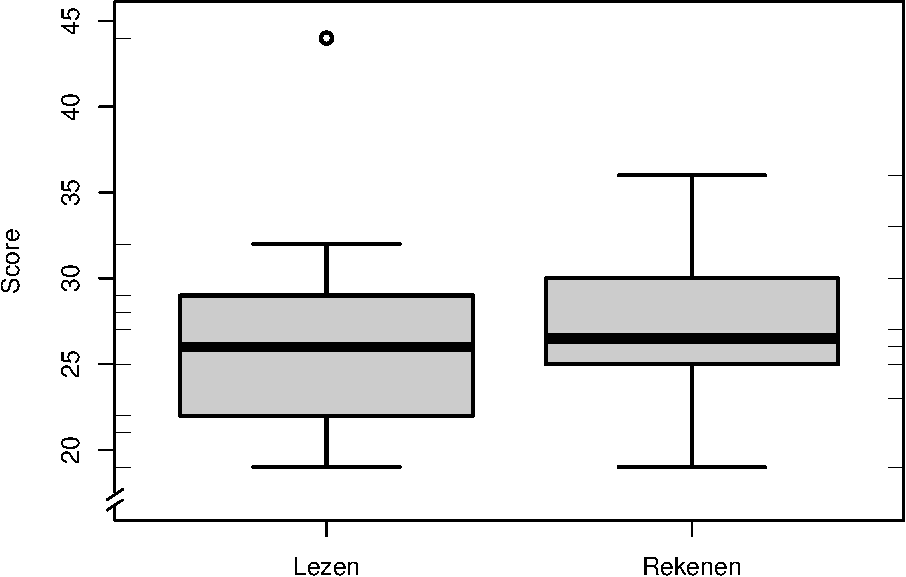
\includegraphics{KMS-NL_files/figure-latex/cito-summary-boxplot-1.pdf}

Veel \textbf{centrummaten} zijn als functie in R voorgeprogrammeerd:

\begin{Shaded}
\begin{Highlighting}[]
\KeywordTok{mean}\NormalTok{(cito}\OperatorTok{$}\NormalTok{Lezen) }\CommentTok{\# gemiddelde}
\end{Highlighting}
\end{Shaded}

\begin{verbatim}
## [1] 27.2
\end{verbatim}

\begin{Shaded}
\begin{Highlighting}[]
\NormalTok{psych}\OperatorTok{::}\KeywordTok{winsor.mean}\NormalTok{(cito}\OperatorTok{$}\NormalTok{Lezen, }\DataTypeTok{trim=}\NormalTok{.}\DecValTok{1}\NormalTok{) }\CommentTok{\# gewinsoriseerde gemiddelde, uit psych package}
\end{Highlighting}
\end{Shaded}

\begin{verbatim}
## [1] 26.3
\end{verbatim}

\begin{Shaded}
\begin{Highlighting}[]
\KeywordTok{mean}\NormalTok{(cito}\OperatorTok{$}\NormalTok{Lezen, }\DataTypeTok{trim=}\NormalTok{.}\DecValTok{1}\NormalTok{) }\CommentTok{\# getrimde gemiddelde}
\end{Highlighting}
\end{Shaded}

\begin{verbatim}
## [1] 26.125
\end{verbatim}

\begin{Shaded}
\begin{Highlighting}[]
\KeywordTok{median}\NormalTok{(cito}\OperatorTok{$}\NormalTok{Lezen)   }\CommentTok{\# mediaan}
\end{Highlighting}
\end{Shaded}

\begin{verbatim}
## [1] 26
\end{verbatim}

Ook diverse \textbf{spreidingsmaten} zijn voorgeprogrammeerd:

\begin{Shaded}
\begin{Highlighting}[]
\KeywordTok{var}\NormalTok{(cito}\OperatorTok{$}\NormalTok{Lezen)  }\CommentTok{\# variantie}
\end{Highlighting}
\end{Shaded}

\begin{verbatim}
## [1] 50.17778
\end{verbatim}

\begin{Shaded}
\begin{Highlighting}[]
\KeywordTok{sd}\NormalTok{(cito}\OperatorTok{$}\NormalTok{Lezen)   }\CommentTok{\# standaarddeviatie, sd(x) = sqrt(var(x))}
\end{Highlighting}
\end{Shaded}

\begin{verbatim}
## [1] 7.083627
\end{verbatim}

\begin{Shaded}
\begin{Highlighting}[]
\KeywordTok{mad}\NormalTok{(cito}\OperatorTok{$}\NormalTok{Lezen)  }\CommentTok{\# MAD}
\end{Highlighting}
\end{Shaded}

\begin{verbatim}
## [1] 5.1891
\end{verbatim}

Daarentegen moeten we \textbf{standaardscores} zelf uitrekenen, en zelf bewaren als nieuwe variabele, hier \texttt{zLezen} genoemd (let op de haakjes in de eerste regel):

\begin{Shaded}
\begin{Highlighting}[]
\NormalTok{zLezen \textless{}{-}}\StringTok{ }\NormalTok{(cito}\OperatorTok{$}\NormalTok{Lezen}\OperatorTok{{-}}\KeywordTok{mean}\NormalTok{(cito}\OperatorTok{$}\NormalTok{Lezen)) }\OperatorTok{/}\StringTok{ }\KeywordTok{sd}\NormalTok{(cito}\OperatorTok{$}\NormalTok{Lezen) }\CommentTok{\# z{-}scores}
\KeywordTok{head}\NormalTok{(zLezen) }\CommentTok{\# eerste paar observaties van variabele zLezen}
\end{Highlighting}
\end{Shaded}

\begin{verbatim}
## [1] -1.1575990  0.6776189  2.3716662 -0.3105753  0.1129365 -0.7340872
\end{verbatim}

\hypertarget{ch:kansverdelingen}{%
\chapter{Kansverdelingen}\label{ch:kansverdelingen}}

\hypertarget{sec:kansen}{%
\section{Kansen}\label{sec:kansen}}

Bellen achter het stuur vergroot de kans op een ongeluk \citep{Bhar13}. De
gemiddelde kans op neerslag in Nederland is 7\%. Mijn bestelling heeft
10\% kans om een dag later dan beloofd afgeleverd te worden. Kansen en
waarschijnlijkheden spelen een belangrijke rol in ons dagelijks leven,
en ook in het wetenschappelijk onderzoek. Immers, veel hypothesen zijn
probabilistisch van aard (zie Hoofdstuk \ref{ch:onderzoek}):
de hypothesen doen uitspraken over
een verschil in \emph{kansen} van uitkomsten. Om conclusies te kunnen trekken
ten aanzien van die probabilistische hypothesen hebben we enige kennis
nodig over waarschijnlijkheden, kansberekening, en kansverdelingen.
Daarover gaat dit hoofdstuk.

Laten we ter inleiding eens kijken naar een Nederlands \emph{Scrabble}-spel.
Het spel bevat een zakje met daarin 102 fiches, met op elke fiche een
letter\footnote{Twee van de fiches zijn echter zonder letter; later in deze paragraaf zullen we deze blanco fiches verwijderen uit het zakje.}. Van de 102 fiches zijn er 6 met de letter A. Als ik uit een
vol en goed gemengd zakje één fiche neem, wat is dan de kans dat ik de
letter A tref? Die kans-op-uitkomst-A wordt aangeduid als
\(P(\textrm{A})\), met de \(P\) van \emph{Probabilitas} (Lat. ``kans,
waarschijnlijkheid''), en is te bepalen als
\begin{equation}
    P(\textrm{A})=
    \frac{\textrm{aantal A's}}{\textrm{totaal aantal fiches}}= 
    \frac{6}{102} = 0.0588
  \label{eq:kans-scrabble-1-A}
\end{equation}

De kans op een gebeurtenis wordt uitgedrukt als een proportie, een getal
tussen \(0\) en \(1\), of als een percentage, d.w.z. een proportie in
eenheden van \(1/100\). Een kans kan dus nooit kleiner zijn dan \(0\) en kan
nooit groter zijn dan 1: de kans is immers de verhouding tussen (teller)
aantal specifieke uitkomsten en (noemer) totaal aantal mogelijke
uitkomsten (zie
formule \eqref{eq:kans-scrabble-1-A}), waarbij deze teller nooit groter kan
zijn dan deze noemer \citep{SK01}.

Als twee uitkomsten elkaar wederzijds uitsluiten, zoals bij de
uitkomsten A of B in ons Scrabble-voorbeeld, dan mogen we de kansen van
die uitkomsten \emph{optellen} (somregel). De kans op uitkomst A \emph{of}
uitkomst B (waarbij de uitkomsten A en B elkaar uitsluiten), is de \emph{som}
van \(P(\textrm{A})\) en \(P(\textrm{B})\):
\begin{equation}
    P(\textrm{A of B}) = P(\textrm{A}) + P(\textrm{B})
  \label{eq:kans-somregel}
\end{equation}

\begin{center}\rule{0.5\linewidth}{0.5pt}\end{center}

\begin{quote}
\emph{Voorbeeld 10.1:}
In ons Scrabble-voorbeeld is \(P(\textrm{A})=\frac{6}{102}\) en
\(P(\textrm{B})=\frac{2}{102}\). De kans op uitkomst A-of-B is dan
\(P(\textrm{A of B})=P(\textrm{A})+P(\textrm{B})=6/102+2/102=8/102=.0784\).
\end{quote}

\begin{center}\rule{0.5\linewidth}{0.5pt}\end{center}

Als ik uit een vol en goed gemengd zakje één fiche neem, dan zijn er
twee complementaire uitkomsten mogelijk: ik tref een A, of ik tref
\emph{niet} een A. De uitkomsten sluiten elkaar weer wederzijds uit, dus ook
de kansen op deze uitkomsten mogen we optellen. Bovendien zijn de
uitkomsten complementair, d.w.z. de uitkomst kan alleen maar één van
deze twee mogelijke uitkomsten zijn. De respectievelijke kansen op deze
complementaire gebeurtenissen zijn dan ook complementair, d.w.z. deze
respectievelijke kansen tellen op tot precies \(1\) =100\%
(complementregel). Er is immers 100\% kans dat de uitkomst één van de
twee mogelijke uitkomsten van de trekking is. Als we \(P(\textrm{A})\) al
kennen kunnen we de kans op de complementaire uitkomst makkelijk
uitrekenen:
\begin{align}
    P(\textrm{A}) + P(\textrm{niet-A}) & = & 1\\
    P(\textrm{A}) & = & 1 - P(\textrm{niet-A})\\
    P(\textrm{niet-A}) & = & 1 - P(\textrm{A})
    \label{eq:complementregel}
\end{align}

\begin{center}\rule{0.5\linewidth}{0.5pt}\end{center}

\begin{quote}
\emph{Voorbeeld 10.2:}
In ons Scrabble-voorbeeld is \(P(\textrm{A})=\frac{6}{102}\). De kans op
uitkomst niet-A is dan
\(P(\textrm{niet-A})= 1 - P(\textrm{A}) = 1 - \frac{6}{102} = \frac{96}{102} = .9412\).
\end{quote}

\begin{center}\rule{0.5\linewidth}{0.5pt}\end{center}

Laten we als gedachten-experiment nu een tweede Scrabble-spel pakken, en
daaruit een tweede zakje met fiches pakken, eveneens vol en goed
gemengd. Uit elk zakje nemen we nu blind één letterfiche. Er zijn nu
twee gebeurtenissen of uitkomsten, nl. de uitkomst van de eerste
trekking (uit het eerste zakje), en de uitkomst van de tweede trekking
(uit het tweede zakje). Deze twee uitkomsten sluiten elkaar niet
wederzijds uit, want de twee uitkomsten hebben geen wederzijdse invloed
op elkaar. De uitkomst uit het tweede zakje wordt immers niet beïnvloed
door de uitkomst van het eerste zakje, of omgekeerd. We zeggen dan dat
deze uitkomsten \emph{onafhankelijk} van elkaar zijn. Als de uitkomsten
inderdaad onafhankelijk van elkaar zijn, dan berekenen we de kans op een
combinatie van uitkomsten door de kansen te \emph{vermenigvuldigen}
(productregel). De kans op de combinatie van uitkomst A \emph{en} uitkomst B
(waarbij de uitkomsten A en B onafhankelijk van elkaar zijn), is het
\emph{product} van \(P(\textrm{A})\) en \(P(\textrm{B})\):
\begin{equation}
    P(\textrm{A en B}) = P(\textrm{A}) \times P(\textrm{B})
  \label{eq:kans-productregel}
\end{equation}

\begin{center}\rule{0.5\linewidth}{0.5pt}\end{center}

\begin{quote}
\emph{Voorbeeld 10.3:}
In ons Scrabble-voorbeeld is \(P(\textrm{A})=\frac{6}{102}\) en
\(P(\textrm{B})=\frac{2}{102}\). De kans op uitkomst A bij het eerste
zakje \emph{en} B bij het tweede zakje is dan
\(P(\textrm{A en B})=P(\textrm{A}) \times P(\textrm{B})=\frac{6}{102} \times \frac{2}{102} = .0012\).
\end{quote}

\begin{center}\rule{0.5\linewidth}{0.5pt}\end{center}

\begin{quote}
\emph{Voorbeeld 10.4:}
In ons Scrabble-voorbeeld is \(P(\textrm{klinker})=\frac{38}{102}\). De kans
om een klinker (A, E, I, O, U, Y) te trekken uit het eerste zakje \emph{en}
een klinker uit het tweede zakje is dan
\(P(\textrm{klinker-en-klinker})=P(\textrm{eerste klinker}) \times P(\textrm{tweede klinker})=\frac{38}{102} \times \frac{38}{102} = (\frac{38}{102})^2 = .1388\).
\end{quote}

\begin{center}\rule{0.5\linewidth}{0.5pt}\end{center}

\hypertarget{sec:binomiaalverdeling}{%
\section{Binomiale kansverdeling}\label{sec:binomiaalverdeling}}

Voor het vervolg van dit hoofdstuk brengen we twee wijzigingen aan in
het Scrabble-spel. Ten eerste verwijderen we de 2 blanco fiches zonder
letter uit het zakje. Er blijven dan precies 100 fiches over, waarvan 38
met een klinker (vocaal, \(V\)) en 62 met een medeklinker (consonant,
\(C\)). Er blijven dus slechts twee mogelijke categorieën van uitkomsten
over, die elkaar wederzijds uitsluiten. Zo'n variabele van het nominale
meetnivo, met precies twee categorieën, noemen we bi-nomiaal
(`twee-namig'). We beschouwen de klinkers als treffers, en de
medeklinkers als missers. Deze twee mogelijke uitkomsten zijn
complementair: \(P(V)=.38\) (afgekort als \(p\)) en \(P(C)=.62\) (afgekort als
\(q=1-p\)).

Ten tweede leggen we het getrokken letterfiche voortaan terug in het
zakje, nadat we de getrokken letter genoteerd hebben. Op die manier
hebben we niet tientallen complete letterzakjes nodig, maar slechts één
letterzakje dat na elke teruglegging weer compleet en goed gemengd is.
We beschouwen de uitkomsten van opeenvolgende trekkingen als
onafhankelijk.

\textbf{Terzijde:} De uitkomst van een bepaalde trekking is dus onafhankelijk
van de uitkomst van vorige trekkingen. Als er zojuist \(100\times\)
achtereen een klinker getrokken is, dan heeft dat geen enkele invloed op
(de uitkomst van) de eerstvolgende trekking uit het letterzakje. Het
letterzakje, of de hand van de trekker, heeft immers geen geheugen. Bij
\emph{elke} trekking is de kans op een treffer \(p=.38\), ook als er zojuist
\(100\times\) of \(1000\times\) een klinker is getrokken. Hetzelfde geldt
voor de opeenvolgende uitkomsten bij roulette: bij elke ronde is de kans
op een treffer \(1/37\), ook als het balletje zojuist \(100\times\) op
eenzelfde getal terecht is gekomen\footnote{Roulettespelers kunnen gokken op 36 van de 37 mogelijke uitkomsten, dus op de lange termijn ontvangt het casino \(1/37\) deel van alle inzetten.}.

Laten we met bovengenoemde wijzigingen nu \(n=3\) trekkingen uitvoeren
(met teruglegging, zie boven), en voor elke mogelijke uitkomst de kans
op die uitkomst bepalen, zie
Tabel \ref{tab:klinkerkansen}.

\begin{longtable}[]{@{}lcc@{}}
\caption{\label{tab:klinkerkansen} Kansen van mogelijke uitkomsten van \(n=3\) trekkingen van klinkers,
\(p=.38\), met teruglegging (zie tekst).}\tabularnewline
\toprule
uitkomst & aantal klinkers & kans\tabularnewline
\midrule
\endfirsthead
\toprule
uitkomst & aantal klinkers & kans\tabularnewline
\midrule
\endhead
CCC & 0 & \(qqq = q^3\)\tabularnewline
VCC & 1 & \(pqq = pq^2\)\tabularnewline
CVC & 1 & \(qpq = pq^2\)\tabularnewline
CCV & 1 & \(qqp = pq^2\)\tabularnewline
VVC & 2 & \(ppq = p^2q\)\tabularnewline
VCV & 2 & \(pqp = p^2q\)\tabularnewline
CVV & 2 & \(qpp = p^2q\)\tabularnewline
VVV & 3 & \(ppp = p^3\)\tabularnewline
\bottomrule
\end{longtable}

Het aantal treffers (klinkers) in de \(n=3\) trekkingen heeft de
\emph{kansverdeling} zoals samengevat in
Tabel \ref{tab:binomkansverdeling3} (eerste en laatste kolom) en
Figuur \ref{fig:binomkansverdeling3} (horizontale en verticale as).
In zo'n kansverdeling zien we voor elke mogelijke uitkomst van \(x\) (hier:
aantal klinkers) hoe groot de kans op die uitkomst is.

\begin{longtable}[]{@{}lrc@{}}
\caption{\label{tab:binomkansverdeling3} Kansverdeling van een binomiale variabele met \(n=3\) en \(p=.38\).}\tabularnewline
\toprule
aantal klinkers & kans & kans\tabularnewline
\midrule
\endfirsthead
\toprule
aantal klinkers & kans & kans\tabularnewline
\midrule
\endhead
0 & \(1 q^3\) & = .2383\tabularnewline
1 & \(3 p q^2\) & = .4383\tabularnewline
2 & \(3 p^2 q\) & = .2686\tabularnewline
3 & \(1 p^3\) & = .0549\tabularnewline
som & \((p+q)^3\) & = 1.0000\tabularnewline
\bottomrule
\end{longtable}

\begin{figure}
\centering
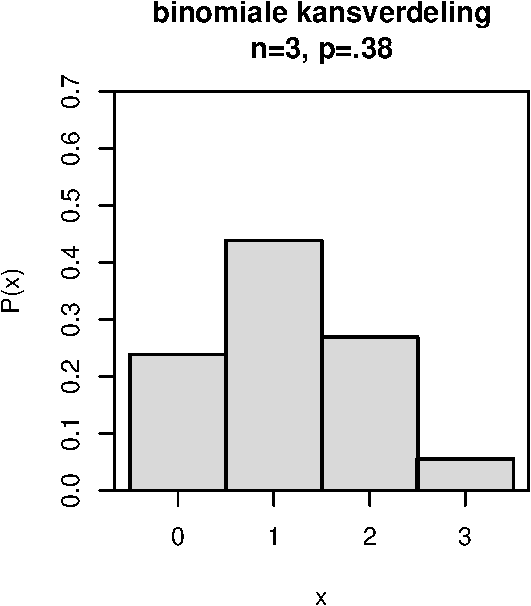
\includegraphics{KMS-NL_files/figure-latex/binomkansverdeling3-1.pdf}
\caption{\label{fig:binomkansverdeling3}Kansverdeling van een binomiale variabele x met n=3 en p=.38.}
\end{figure}

De kansverdeling van een binomiale variabele noemen we de binomiale
kansverdeling, ook aangeduid als binomiale verdeling of
binomiaalverdeling. De exacte kansen van de binomiale kansverdeling kan
je uitrekenen met formule \eqref{eq:prob-binomial} hieronder.

\hypertarget{formules}{%
\subsection{formules}\label{formules}}

De kans op een \(x\) aantal treffers in \(n\) trekkingen is gegeven als
\begin{equation}
  P(x\,\mbox{treffers}) = {n \choose x} p^x (1-p)^{n-x}
  \label{eq:prob-binomial}
\end{equation}
waarbij \(n\) is het aantal trekkingen of pogingen, \(x\) is het aantal treffers (tussen
0 en \(n\)), en \(p\) is de kans op een treffer.

De coëfficient \({n \choose x}\) geeft het aantal verschillende ordeningen
aan waarin we een combinatie (greep) van \(x\) elementen uit \(n\) kunnen
kiezen. Bij \(x=1\) klinker uit \(n=3\) trekkingen zijn er drie
mogelijkheden: de ene klinker zou getrokken kunnen zijn in de eerste
trekking, of de tweede trekking, of de derde trekking, zie
Tabel \ref{tab:klinkerkansen}. Het aantal verschillende mogelijke
ordeningen is gegeven als
\begin{equation}
  {n \choose x} = \frac{n!}{x!(n-x)!}
  \label{eq:choose}
\end{equation}
waarbij
\(x! = x (x-1) (x-2) \dots \times 2 \times 1\), dus
\(4!=4\times3\times2\times1=24\).

\begin{center}\rule{0.5\linewidth}{0.5pt}\end{center}

\begin{quote}
\emph{Voorbeeld 10.5:} Er staan 4 stoelen voor 2 personen. Op een stoel mag maximaal 1 persoon
plaatsnemen. Hoeveel verschillende ordeningen van \(x=2\) personen over
\(n=4\) stoelen zijn er mogelijk?
\end{quote}

\begin{quote}
Antwoord: Er zijn
\({4 \choose 2} = \frac{4\times3\times2\times1}{2\times1\times2\times1} = \frac{24}{4} = 6\)
mogelijke ordeningen, namelijk 1100, 1010, 1001, 0110, 0101, en 0011.
\end{quote}

\begin{center}\rule{0.5\linewidth}{0.5pt}\end{center}

Deze binomiaal-coëfficienten, die het aantal verschillende mogelijke
ordeningen aangeven, zijn snel terug te vinden in de zogenaamde Driehoek
van Pascal, afgebeeld in Tabel \ref{tab:driehoekpascal}.
Het aantal verschillende
ordeningen van \(x=2\) personen over \(n=4\) stoelen vinden we in rij \(n=4\).
De bovenste rij is die voor \(n=0\). De vijfde rij is die voor \(n=4\) en we
zien daar achtereenvolgens de binomiaal-coëfficienten voor
\(x= 0, 1, 2, 3, 4\). Voor \({4 \choose 2}\) vinden we daar de
binomiaalcoëfficient \(6\). Iedere coefficiënt is de som van de twee
bovenliggende coëfficienten\footnote{Dus \({n \choose x} = {n-1 \choose x} + {n-1 \choose x-1}\), \citep{Weis15}.}, en iedere coëfficient is op te vatten
als het aantal mogelijke wegen afdalend van de top van de driehoek naar
die cel.

\begin{longtable}[]{@{}llllllllclllllll@{}}
\caption{\label{tab:driehoekpascal} Driehoek van Pascal: binomiaalcoëfficienten voor het aantal mogelijke ordeningen voor een combinatie van \(x\) elementen uit \(n\) (zie tekst).}\tabularnewline
\toprule
\endhead
\(n= 0\): & & & & & & & & 1 & & & & & & &\tabularnewline
\(n= 1\): & & & & & & & 1 & & 1 & & & & & &\tabularnewline
\(n= 2\): & & & & & & 1 & & 2 & & 1 & & & & &\tabularnewline
\(n= 3\): & & & & & 1 & & 3 & & 3 & & 1 & & & &\tabularnewline
\(n= 4\): & & & & 1 & & 4 & & 6 & & 4 & & 1 & & &\tabularnewline
\(n= 5\): & & & 1 & & 5 & & 10 & & 10 & & 5 & & 1 & &\tabularnewline
\(n= 6\): & & 1 & & 6 & & 15 & & 20 & & 15 & & 6 & & 1 &\tabularnewline
\(n= 7\): & 1 & & 7 & & 21 & & 35 & & 35 & & 21 & & 7 & & 1\tabularnewline
\bottomrule
\end{longtable}

Het gemiddelde en de standaarddeviatie van de binomiale kansverdeling
zijn \[\begin{aligned}
    \mu & = & np \\
    \sigma & = & \sqrt{ np(1-p) }\end{aligned}\]

\begin{center}\rule{0.5\linewidth}{0.5pt}\end{center}

\begin{quote}
\emph{Voorbeeld 10.6:}
De binomiale kansverdeling voor \(x\) treffers uit \(n=3\) trekkingen met
\(p=.38\) kans op een treffer is afgebeeld in
Figuur \ref{fig:binomkansverdeling3}. Deze binomiale kansverdeling heeft
een gemiddelde \(\mu=n \times p = 3 \times .38 = 1.14\), en een
standaarddeviatie
\(\sigma = \sqrt{n \times p \times (1-p)} = \sqrt{ 3 \times .38 \times .62} = 0.84\)
.
\end{quote}

\begin{center}\rule{0.5\linewidth}{0.5pt}\end{center}

\hypertarget{r-4}{%
\subsection{R}\label{r-4}}

\begin{Shaded}
\begin{Highlighting}[]
\KeywordTok{dbinom}\NormalTok{( }\DecValTok{0}\OperatorTok{:}\DecValTok{3}\NormalTok{, }\DataTypeTok{size=}\DecValTok{3}\NormalTok{, }\DataTypeTok{prob=}\NormalTok{.}\DecValTok{38}\NormalTok{ )}
\end{Highlighting}
\end{Shaded}

\begin{verbatim}
## [1] 0.238328 0.438216 0.268584 0.054872
\end{verbatim}

De uitvoer is weergegeven in Tabel \ref{tab:binomkansverdeling3} hierboven.

\begin{Shaded}
\begin{Highlighting}[]
\NormalTok{matrixcalc}\OperatorTok{::}\KeywordTok{pascal.matrix}\NormalTok{( }\DecValTok{10}\NormalTok{ ) }\CommentTok{\# links onder diagonaal is Driehoek van Pascal}
\end{Highlighting}
\end{Shaded}

\begin{verbatim}
##       [,1] [,2] [,3] [,4] [,5] [,6] [,7] [,8] [,9] [,10]
##  [1,]    1    0    0    0    0    0    0    0    0     0
##  [2,]    1    1    0    0    0    0    0    0    0     0
##  [3,]    1    2    1    0    0    0    0    0    0     0
##  [4,]    1    3    3    1    0    0    0    0    0     0
##  [5,]    1    4    6    4    1    0    0    0    0     0
##  [6,]    1    5   10   10    5    1    0    0    0     0
##  [7,]    1    6   15   20   15    6    1    0    0     0
##  [8,]    1    7   21   35   35   21    7    1    0     0
##  [9,]    1    8   28   56   70   56   28    8    1     0
## [10,]    1    9   36   84  126  126   84   36    9     1
\end{verbatim}

De driehoek van Pascal is te vinden links onder de diagonaal van deze matrix.

\hypertarget{sec:normaalverdeling}{%
\section{Normale kansverdeling}\label{sec:normaalverdeling}}

Naarmate de steekproefgrootte \(n\) toeneemt, gaat de binomiale
kansverdeling minder trapsgewijs verspringen, en wordt de kansverdeling
meer vloeiend, zoals te zien in
Figuur \ref{fig:binomkansverdeling50n500}.

\begin{figure}
\centering
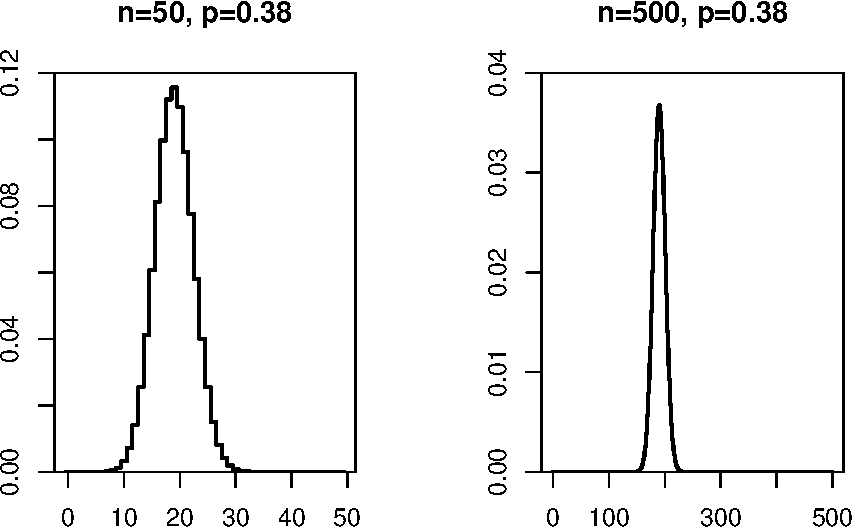
\includegraphics{KMS-NL_files/figure-latex/binomkansverdeling50n500-1.pdf}
\caption{\label{fig:binomkansverdeling50n500}Kansverdeling van een binomiale variabele x met n=50 (links) en n=500 (rechts) en p=.38.}
\end{figure}

Bij een nog grotere steekproef wordt de kansverdeling een vloeiende lijn.
Deze kansverdeling komt zo vaak voor, dat dit de \emph{normale kansverdeling}
of `normale verdeling' wordt genoemd. De verdeling wordt ook wel
aangeduid als de Gaussische verdeling (vernoemd naar de wiskundige Carl
Friedrich Gauss, 1777--1855), of de `bell curve' (naar de vorm). Heel
veel variabelen volgen bij benadering deze kansverdeling:
geboortegewicht, lichaamslengte, omvang van woordenschat, IQ, inhoud van
een pak melk van 1 liter ℮, duur van een telefoongesprek, enz enz. Voor
al deze variabelen hebben observaties dicht bij het gemiddelde een hoge
kans om voor te komen, en observaties die sterk afwijken van het
gemiddelde zijn relatief zeldzaam (lage kans).

\begin{figure}
\centering
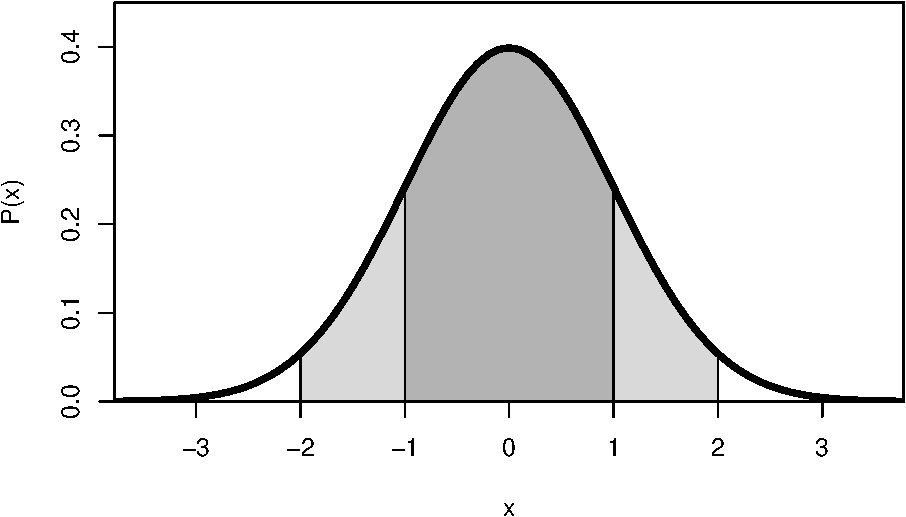
\includegraphics{KMS-NL_files/figure-latex/normaalkansverdeling-1.pdf}
\caption{\label{fig:normaalkansverdeling}Normale kansverdeling van een variabele x met gemiddelde 0 en standaarddeviatie 1.}
\end{figure}

De normale kansverdeling van variabele \(X\) met gemiddelde \(\mu\) en
standaarddeviatie \(\sigma\) heeft de volgende kenmerken (zie
Figuur \ref{fig:normaalkansverdeling}):

\begin{itemize}
\item
  de verdeling is symmetrisch rond het gemiddelde \(\mu\),
\item
  de verdeling is asymptotisch, d.w.z. de staarten lopen eindeloos
  door,
\item
  het gemiddelde, de mediaan en de modus vallen samen,
\item
  de totale oppervlakte onder de curve, d.i. de totale kans op één van
  de mogelijke uitkomsten, is gelijk aan 1,
\item
  de oppervlakte onder de curve geeft de kans aan op een waarde van \(X\) binnen een bepaald interval,
\item
  de buigpunten van de curve (van hol naar bol en v.v.) liggen bij
  \(X=\mu-\sigma\) en \(X=\mu+\sigma\),
\item
  ongeveer 2/3 van de observaties ligt
  tussen \(X=\mu-\sigma\) en \(X=\mu+\sigma\) (donkergrijs gebied;
  \(P(-1<x/\sigma<1)=.6827\) of 68\%) en ongeveer 95\% van de observaties ligt
  tussen \(-2\sigma\) en \(+2\sigma\) (donkergrijs plus lichtgrijze
  gebieden; \(P(-2<x/\sigma<2)=.9546\)), dit staat bekend als de
  Empirical Rule.
\end{itemize}

Een normale kansverdeling met \(\mu=0\) en \(\sigma=1\) wordt aangeduid als
de standaard-normale kansverdeling. Zoals we al eerder zagen
(§\ref{sec:standaardscores}) kunnen we een normaal-verdeelde
variabele \(x\) standaardiseren, d.w.z. de observaties transformeren naar
een standaardscore of \(z\)-score: \(z = (x-\overline{x})/s\).
De kansverdeling in
Figuur \ref{fig:normaalkansverdeling} is die van de standaard-normale
kansverdeling van \(Z\), oftewel de kansverdeling van \((X-\mu)/\sigma\).

De kansverdeling van een normaal verdeelde variabele \(X\) zou je zelf
kunnen uitrekenen met behulp van formule
\eqref{eq:prob-normal} hieronder. Maar het is handiger om daarvoor
een tabel te gebruiken; die staat in
Bijlage \ref{app:kritiekeZwaarden}.
In grafische vorm uitgelegd geven die tabellen je,
voor verschillende oppervlakten ofwel kansen \(p\) aan de rechter zijde onder de curve,
de positieve waarde van \(Z^*\) die de linkergrens vormt
van die oppervlakte. Dat betekent dus dat je precies de kans \(p\) hebt om
een waarde te vinden van \(Z\) die even groot als of groter dan deze
ondergrens \(Z^*\) is (mits de variabele inderdaad normaal verdeeld is).

\begin{center}\rule{0.5\linewidth}{0.5pt}\end{center}

\begin{quote}
Voorbeeld 10.7: Aan de rechterzijde van Figuur \ref{fig:normaalkansverdeling} zien we een klein wit oppervlak onder de curve. Dit oppervlak geeft de kans weer dat \(Z>2\). Het oppervlak heeft een omvang van 0.0228. De kans om een waarde van \(Z>2\) te vinden is dus 0.0228 ofwel iets minder dan 2.5\%. (Tip: relateer deze kans aan de bovengenoemde Empirical Rule).
\end{quote}

\begin{center}\rule{0.5\linewidth}{0.5pt}\end{center}

In
Bijlage \ref{app:kritiekeZwaarden} vind je gemakshalve niet een maar twee
tabellen, elk bestaande uit meerdere kolom-aanduidingen en één rij van
cellen. De eerste tabel geeft je, voor verschillende `afgeronde' kansen
\(p\) (kolommen), de kritieke waarde \(Z^*\) (cellen) waarvoor geldt dat de
kans \(p\) om een waarde van \(Z\) te vinden die even groot als of groter
dan deze kritieke waarde \(Z^*\) is, precies gelijk is aan de waarde \(p\)
bovenaan de kolom. De tweede tabel werkt net zo, maar dan voor
`afgeronde' waarden van \(Z^*\) in de cellen, en precieze kansen \(p\) in de
kolom-aanduidingen.

Wat is de kans \(p\) dat \(Z>1\)? In de tweede deeltabel, tweede kolom,
vinden we \(p=0.1587\). We weten daarmee ook dat \(P(Z<1)\) wel
\(1-0.1587=0.8413\) moet zijn. Bovendien weten we dat de verdeling
symmetrisch is (zie hierboven), dus weten we dat \(P(Z< -1)\) ook \(.1587\)
moet zijn. Wat is de kans \(p\) dat \(Z>3\) is? In de tweede deeltabel
vinden we voor grenswaarde \(Z^*=3\) de overschrijdingskans
\(p=0.0013\). Voor een normaal verdeelde variabele \(Z\) is er dus een
overschrijdingskans \(p=0.0013\) om een waarde van \(Z\) te vinden die
tenminste drie standaarddeviaties boven het gemiddelde ligt.

Vaak willen we het omgekeerde weten: als we een bepaalde
overschrijdingskans kiezen, welke grenswaarde \(Z^*\) hoort daar dan bij?
Welke grenswaarde onderscheidt de hoogste 5\% van de observaties van de
onderste 95\% (\(p=0.05\))? In de eerste deeltabel vinden we
voor overschrijdingskans \(p=0.05\) de grenswaarde \(Z^*=1.645\). Deze
grenswaarde, teruggerekend naar de oorspronkelijke variabele, wordt dan
vaak aangeduid als het 95e percentiel of `P95' van de verdeling. Wie
tenminste deze score heeft behaald, behoort bij de beste 5\% en heeft het dus
beter gedaan dan 95\% van de deelnemers.

\begin{center}\rule{0.5\linewidth}{0.5pt}\end{center}

\begin{quote}
\emph{Voorbeeld 10.8:}
Extreme waarden komen bij een normaal-verdeelde variabele per definitie
weinig voor. Maar wat is de grens voor een extreme waarde? Laten we
aannemen dat we niet meer dan 5\% van alle observaties als extreem willen
beschouwen. De normale kansverdeling is symmetrisch, dus van die 5\% is
te verwachten dat de ene helft (2.5\%) ligt aan het linker uiteinde van
de verdeling, en de andere 2.5\% aan de rechterzijde. Welke grenswaarde
\(Z^*\) correspondeert met deze overschrijdingskans \(p=0.025\)?
\end{quote}

\begin{quote}
In
Bijlage \ref{app:kritiekeZwaarden} nemen we de eerste deeltabel. In de kolom
voor overschrijdingskans \(p=0.025\), vinden we grenswaarde
\(Z^*=1.960\). Als we een observatie vinden met \(Z \ge 1.960\) of met
\(Z \le -1.960\) dan beschouwen we dat als een extreme, zeldzame
observatie.
\end{quote}

\begin{center}\rule{0.5\linewidth}{0.5pt}\end{center}

\begin{quote}
\emph{Voorbeeld 10.9:}
Intelligentie wordt uitgedrukt als een IQ-score, een variabele met een
normale kansverdeling met \(\mu=100\) en \(\sigma=15\). ``Membership of Mensa
is open to persons who have attained a score within the upper two
percent of the general population on an approved intelligence test that
has been properly administered and supervised''
(\url{www.mensa.org}). Welke IQ-score moet je tenminste
behalen om lid te kunnen worden?
\end{quote}

\begin{quote}
Antwoord: Het 98e percentiel van een standaard-normaal verdeelde
variabele ligt bij \(Z^*=+2.0537\), en dus met
\(x=\overline{x}+2.0537 s = 100+30.8 = 130.8\). Naar boven afgerond moet
je dus een IQ-score behalen van 131 punten of hoger.
\end{quote}

\begin{center}\rule{0.5\linewidth}{0.5pt}\end{center}

\begin{quote}
\emph{Voorbeeld 10.10:}
Verifieer de bovengenoemde Empirical Rule met behulp van
Bijlage \ref{app:kritiekeZwaarden}.
\end{quote}

\begin{center}\rule{0.5\linewidth}{0.5pt}\end{center}

\hypertarget{formules-1}{%
\subsection{formules}\label{formules-1}}

Als variabele \(X\) een normale kansverdeling heeft, met gemiddelde \(\mu\)
en standaarddeviatie \(\sigma\), dan wordt dat aangegeven als
\begin{equation}
  X \sim \mathcal{N}(\mu,\sigma)
  \label{eq:normaalverdeeld}
\end{equation}

De normale kansverdeling van variabele \(X\) met gemiddelde \(\mu\) en
standaarddeviatie \(\sigma\) is
\begin{equation}
  P(X) = \frac{1}{\sigma \sqrt{2\pi}} \mbox{e}^{ \frac{-(X-\mu)^2}{2\sigma^2} }.
  \label{eq:prob-normal}
\end{equation}

De standaard-normale kansverdeling van variabele \(Z\) met gemiddelde
\(\mu=0\) en standaarddeviatie \(\sigma=1\) is
\begin{equation}
    P(Z) = \frac{1}{\sqrt{2\pi}} \mbox{e}^{ \frac{-Z^2}{2} }
  \label{eq:prob-standaardnormaal}
\end{equation}

\hypertarget{sec:isvarnormaalverdeeld}{%
\section{Heeft mijn variabele een normale kansverdeling?}\label{sec:isvarnormaalverdeeld}}

Het langste nummer in mijn digitale muziekbibliotheek duurt ongeveer 50
minuten (dat is een klassiek-indiaas muziekstuk, een `morning raga').
Een histogram van de duren van alle muzieknummers zie je in
Figuur \ref{fig:itunestimeshist}.

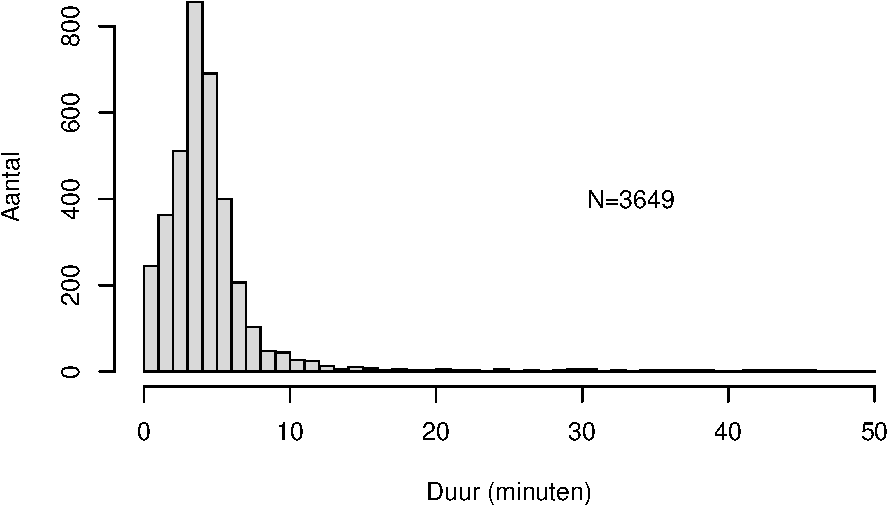
\includegraphics{KMS-NL_files/figure-latex/itunestimeshist-1.pdf}
Dit histogram laat zien dat deze duren
duidelijk \emph{niet} een normale kansverdeling volgen: de verdeling is niet
symmetrisch, en de onderste staart loopt niet eindeloos door (er zijn
geen muzieknummers met negatieve duren).

Ook het gemiddelde \(\bar{x} =\) 4.698 en
standaarddeviatie \(s =\) 5.11
wijzen op een niet-normale kansverdeling:
bij een normale verdeling verwachten we dat slechts \((68/2)+50=84\)\% van de duren langer duurt dan
\(\bar{x}-s\approx 0\) minuten, maar in werkelijkheid duurt 100\%
(dus een groter deel dan verwacht) langer dan 0 minuten.

Een veel gebruikte manier om te inspecteren of een variabele \(X\) een
normale kansverdeling heeft, is om een grafiek te maken met de
geobserveerde waarden langs de ene as (hier de horizontale), en de corresponderende \(z\)-scores
langs de andere as. Zo'n figuur wordt een quantile-quantile-plot of
QQ-plot genoemd; de QQ-plot voor de duren in mijn muziekbibliotheek zie
je in Figuur \ref{fig:itunestimesqqplot}.

\begin{figure}
\centering
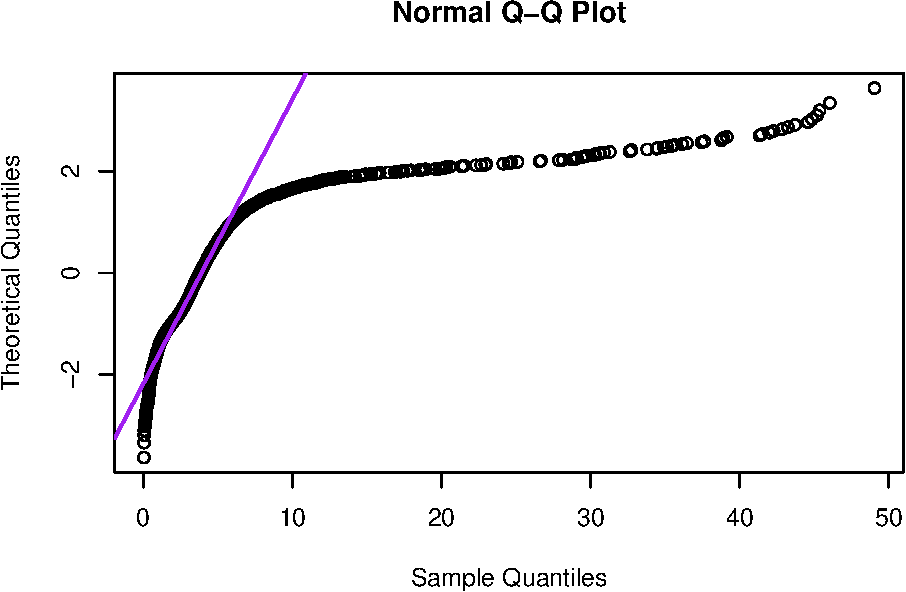
\includegraphics{KMS-NL_files/figure-latex/itunestimesqqplot-1.pdf}
\caption{\label{fig:itunestimesqqplot}Quantile-quantile-plot van de duren van muzieknummers in mijn digitale muziekbibliotheek.}
\end{figure}

Als de duren een normale kansverdeling zouden hebben (normaal zouden
zijn verdeeld), dan zouden er een aantal negatieve duren moeten zijn, en
er zouden dan veel meer duren tussen 8 en 14 minuten moeten zijn (i.p.v.
tussen 8 en 50 minuten). De afwijkingen van de rechte lijn in
Figuur \ref{fig:itunestimesqqplot} geven dus aan dat de geobserveerde
duren niet een normale kansverdeling volgen, zoals we al zagen in het
histogram (Figuur \ref{fig:itunestimeshist}).

Er zijn ook verschillende statistische toetsen om te onderzoeken of een
variabele een normale kansverdeling heeft. De twee meest gebruikte zijn
de Shapiro-Wilk-toets (met toetsingsgrootheid \(W\)) voor normaliteit, en
de Kolmogorov-Smirnov-toets (met toetsingsgrootheid \(D\)) voor
normaliteit. Beide toetsen onderzoeken de
H0:\(X\sim\mathcal{N}(\bar{X},s)\) (zie
formule \eqref{eq:normaalverdeeld}).

\hypertarget{spss-4}{%
\subsection{SPSS}\label{spss-4}}

\begin{verbatim}
Analyze > Descriptive Statistics > Explore...
\end{verbatim}

Selecteer variabele Time (sleep naar Dependent List paneel).\\
Kies knop \texttt{Plots}, en vink aan \texttt{Normality\ plots\ with\ tests}, dat
betekent `als je een QQ-plot oftewel Normality plot maakt, voer dan ook toetsen
op normaliteit uit'. Bevestig met \texttt{Continue} en daarna met \texttt{OK}. De
uitvoer bevat eerst de resultaten van de Shapiro-Wilks-toets en de
Kolmogorov-Smirnov toets. Volgens beide toetsen is de kans om deze
verdeling te vinden, als H0 waar is, bijna nul --- zie echter de
waarschuwing in
§@ref(\#sec:pgroterdannul)! We verwerpen daarom H0 en concluderen
dat de duren van muzieknummers niet normaal verdeeld zijn. Na deze
toetsresultaten volgt o.a. een QQ-plot.

\hypertarget{r-5}{%
\subsection{R}\label{r-5}}

\begin{Shaded}
\begin{Highlighting}[]
\NormalTok{itunes \textless{}{-}}\StringTok{ }\KeywordTok{read.table}\NormalTok{( }\DataTypeTok{file=}\StringTok{"data/itunestimes20120511.txt"}\NormalTok{, }\DataTypeTok{header=}\OtherTok{TRUE}\NormalTok{ )}
\CommentTok{\# Size in bytes, Time in ms}
\KeywordTok{qqnorm}\NormalTok{(itunes}\OperatorTok{$}\NormalTok{Time}\OperatorTok{/}\DecValTok{60000}\NormalTok{, }\DataTypeTok{datax=}\NormalTok{T, }\DataTypeTok{plot.it=}\OtherTok{FALSE}\NormalTok{) }\CommentTok{\# normally we\textquotesingle{}d use plot.it=TRUE  }
\CommentTok{\# qqline(itunes$Time/60000, datax=T, col="purple", lwd=T) \# see QQ{-}plot above}
\end{Highlighting}
\end{Shaded}

\begin{Shaded}
\begin{Highlighting}[]
\KeywordTok{shapiro.test}\NormalTok{(itunes}\OperatorTok{$}\NormalTok{Time}\OperatorTok{/}\DecValTok{60000}\NormalTok{)}
\end{Highlighting}
\end{Shaded}

\begin{verbatim}
## 
##  Shapiro-Wilk normality test
## 
## data:  itunes$Time/60000
## W = 0.50711, p-value < 2.2e-16
\end{verbatim}

Volgens deze toets is de kans om deze verdeling te vinden, als H0 waar
is, bijna nul, nl. kleiner dan \(2.2 \times 10^{-16}\) (d.i. kleiner dan
het kleinste getal dat het analysepakket hier kan weergeven). We
verwerpen daarom H0 en concluderen dat de duren van muzieknummers niet
normaal verdeeld zijn.

\hypertarget{sec:watalsnietnormaal}{%
\section{Wat als mijn variabele niet normaal verdeeld is?}\label{sec:watalsnietnormaal}}

In Deel III zullen we diverse statistische
toetsen bespreken. De toetsen die we bespreken in hoofdstukken
\ref{ch:toetsing} en \ref{ch:power} en \ref{ch:variantieanalyse}
vereisen echter dat de afhankelijke
variabele een normale kansverdeling heeft. Als een variabele \emph{niet} een
(ongeveer) normale kansverdeling heeft, dan kan die variabele dus niet
zomaar gebruikt worden voor statistische toetsing met de daar behandelde
statistische toetsen, of exacter gezegd, de conclusies uit zo'n
statistische toetsing zijn dan niet valide. Wat te doen? Er zijn dan
twee mogelijkheden.

Ten eerste is het mogelijk om de afhankelijke variabele \(y\) te
transformeren, d.w.z. dat we er een rekenkundige bewerking op loslaten.
Als het goed is, resulteert dat in een variabele \(y'\) die wèl bij
benadering normaal verdeeld is. Veel gebruikte transformaties zijn:
logaritmiseren (\(y'=\log{y}\)), worteltrekken (\(y'=\sqrt{y}\)), of
inverteren (\(y'=1/y\)). Vervolgens wordt de getransformeerde
afhankelijke variabele \(y'\) gebruikt voor de statistische toetsing.
Uiteraard moet je wel controleren of de nieuwe afhankelijke variabele
\(y'\) inderdaad (bij benadering) normaal verdeeld is. Ook moet je bij de
interpretatie van de resultaten van de analyse rekening houden met de
uitgevoerde transformatie!

Ten tweede is het soms mogelijk om een andere statistische toets te
gebruiken, die niet vereist dat de afhankelijke variabele normaal
verdeeld is. Dat worden non-parametrische toetsen genoemd. We gaan er
nader op in in de hoofdstukken \ref{ch:chi-kwadraat-toetsen} en
\ref{ch:andere-nonpar-toetsen}.
Die toetsen hebben wel als nadeel
dat ze minder statistische power hebben (voor een bespreking van power,
zie hoofdstuk \ref{ch:power}): ze zijn minder gevoelig, en vereisen dus grotere
steekproeven om een effect vast te stellen.

\hypertarget{sec:CentraalLimietTheorema}{%
\section{Kansverdeling van gemiddelde}\label{sec:CentraalLimietTheorema}}

In deze paragraaf beschouwen we de muzieknummers in mijn digitale
muziekbibliotheek als een \emph{populatie}. We nemen nu een willekeurige
steekproef van \(n=\) 50 nummers, en bepalen de gemiddelde duur over deze
50 muzieknummers in de steekproef:
stel \(\bar{x} =\) 4.401 minuten. Opvallend
genoeg ligt dit gemiddelde van de steekproef dicht bij het gemiddelde
van de populatie (\(\mu =\) 4.615 minuten, zie hierboven).
Deze operatie herhalen we
\(250\times\): we krijgen zo 250 steekproefgemiddelden. De
frequentieverdeling van die 250 steekproefgemiddelden zie je in
Figuur \ref{fig:itunesmeanshist}.

\begin{figure}
\centering
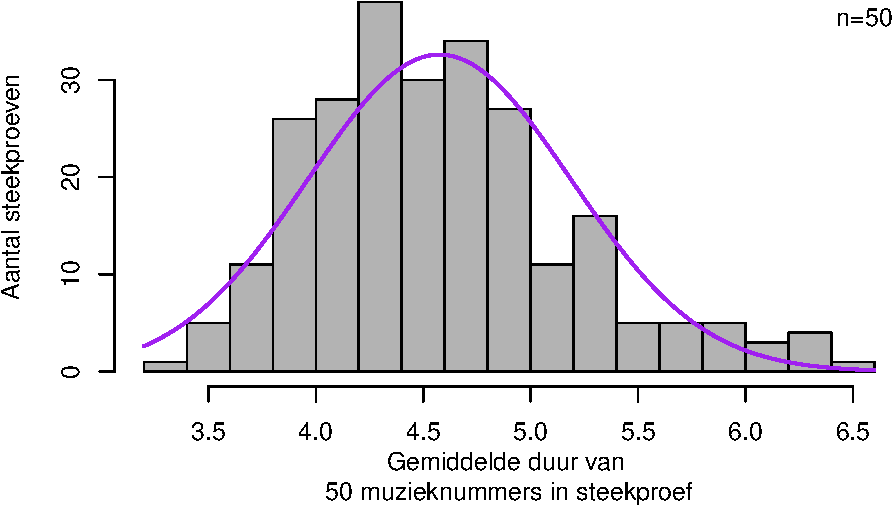
\includegraphics{KMS-NL_files/figure-latex/itunesmeanshist-1.pdf}
\caption{\label{fig:itunesmeanshist}Frequentieverdeling van 250 gemiddelden, elk over een willekeurige steekproef van \(n=50\) muzieknummers (de afhankelijke variabele is de duur van een muzieknummer, in minuten). De bijpassende normaalverdeling is aangegeven als een vloeiende curve.}
\end{figure}

Opvallend genoeg vertonen deze \emph{gemiddelden} van (de afhankelijke
variabele \(X\) in) de steekproeven \emph{wel} een min of meer normale kansverdeling, of de
variabele \(X\) in de populatie nu wel of niet normaal verdeeld is. Anders
gezegd, de kansverdeling van een steekproefgemiddelde benadert \emph{altijd} de
normale kansverdeling, ongeacht de kansverdeling van de betreffende
variabele in de populatie, indien tenminste de steekproef voldoende
groot was. (Dit staat bekend als het Centraal Limiet Theorema). Lees de
bovenstaande zinnen nog eens aandachtig door. Als vuistregel geldt dat
de omvang van de steekproef, \(n\), tenminste 30 moet zijn. Naarmate de
steekproef groter is, wijkt de kansverdeling van de
steekproefgemiddelden minder af van de normaalverdeling.

De normale kansverdeling van de steekproefgemiddelden heeft een eigen
gemiddelde, \(\mu_{\bar{X}}\), en een eigen standaarddeviatie,
\(s_{\bar{X}}\). Hiervoor geldt:
\begin{equation}
    \mu_{\bar{X}} = \mu_X
    \label{eq:meanofmean}
\end{equation}
en
\begin{equation}
    s_{\bar{X}} = \frac{s}{\sqrt{n}}
    \label{eq:sem}
\end{equation}
De standaarddeviatie van het
gemiddelde, \(s_{\bar{X}}\), staat ook bekend als de `standard error of
the mean'. De steekproefgemiddelden \(\bar{X}\) hebben minder spreiding
dan de afzonderlijke observaties \(X\), en de gemiddelden variëren ook
minder naarmate er gemiddeld is over een grotere steekproef, zoals ook
blijkt uit formule \eqref{eq:sem}. Je kunt deze standard error of the mean goed
beschouwen als de `foutmarge' bij de schatting van het
populatiegemiddelde uit het steekproefgemiddelde.

Het bijzondere is nu, dat we niet 250 herhaalde willekeurige
steekproeven hoeven te trekken en te analyseren. We weten immers dat de
steekproefgemiddelden een normale kansverdeling hebben met
\(\mu_{\bar{X}} = \mu_X\) en \(s_{\bar{X}} = \frac{s}{\sqrt{n}}\). De
kansverdeling van het gemiddelde kunnen we dus afleiden uit slechts één
steekproef van \(n\) observaties, met één steekproefgemiddelde \(\bar{X}\)
en één standaarddeviatie \(s\) \citep{Cumm12}. Lees ook deze alinea nog eens
aandachtig door.

\hypertarget{sec:betrouwbaarheidsinterval-gemiddelde}{%
\section{Betrouwbaarheidsinterval van het gemiddelde}\label{sec:betrouwbaarheidsinterval-gemiddelde}}

Zoals hierboven uitgelegd, kunnen we het gemiddelde van de steekproef,
\(\bar{X}\), gebruiken als een goede schatting van het onbekende
gemiddelde in de populatie, \(\mu\). Op grond van het Centraal Limiet
Theorema (§\ref{sec:CentraalLimietTheorema}) weten we ook dat de gemiddelden
van herhaalde steekproeven (van \(n\) observaties) een normale verdeling
volgen: \(\mu_{\bar{X}} \sim \mathcal{N}(\mu_{X},\sigma/\sqrt{n})\), en
dus dat 95\% van deze herhaalde steekproefgemiddelden zullen liggen
tussen \(\mu_{X}-1.96\sigma/\sqrt{n}\) en \(\mu_{X}+1.96\sigma/\sqrt{n}\).
Dit interval wordt het 95\%-betrouwbaarheidsinterval genoemd. We weten
met 95\% betrouwbaarheid dat het populatiegemiddelde \(\mu\) in dit
interval ligt --- mits \(n\) voldoende groot is, en mits de
standaarddeviatie, \(\sigma\), in de populatie bekend is.

Aan die laatste voorwaarde wordt in de praktijk echter zelden of nooit
voldaan. De standaarddeviatie in de populatie is doorgaans niet bekend,
en deze \(\sigma\) wordt daarom ook geschat uit de steekproef. We
gebruiken de steekproef van \(n\) observaties dus niet alleen om \(\mu_X\)
te schatten, maar ook om \(\sigma_X\) te schatten. We mogen dan het
betrouwbaarheidsinterval niet meer bepalen op grond van de
standaard-normale kansverdeling. In plaats daarvan gebruiken we een
aangepaste versie daarvan, de zgn. \(t\)-verdeling
(Figuur \ref{fig:tkansverdeling}). Deze kansverdeling van \(t\) is iets
breder, d.w.z. met een iets lagere top en met iets dikkere staarten, dan
de standaard-normale kansverdeling van \(Z\) in
Figuur \ref{fig:normaalkansverdeling}.
De gedachte daarbij is dat de
schatting van \(\mu\) wat onzekerder is (dus de kansverdeling is breder)
omdat niet alleen \(\mu\) maar ook de standard error of the mean
(\(s/\sqrt{n}\)) geschat wordt op grond van de steekproef. In allebei de
schattingen kunnen afwijkingen zitten, waardoor iets meer kans is om een
steekproefgemiddelde te vinden dat afwijkt van het populatiegemiddelde.
Zoals we al zagen wordt de schatting van \(\mu\) beter naarmate \(n\) groter
is: de \(t\)-verdeling benadert dan de standaard-normale kansverdeling.

\begin{figure}
\centering
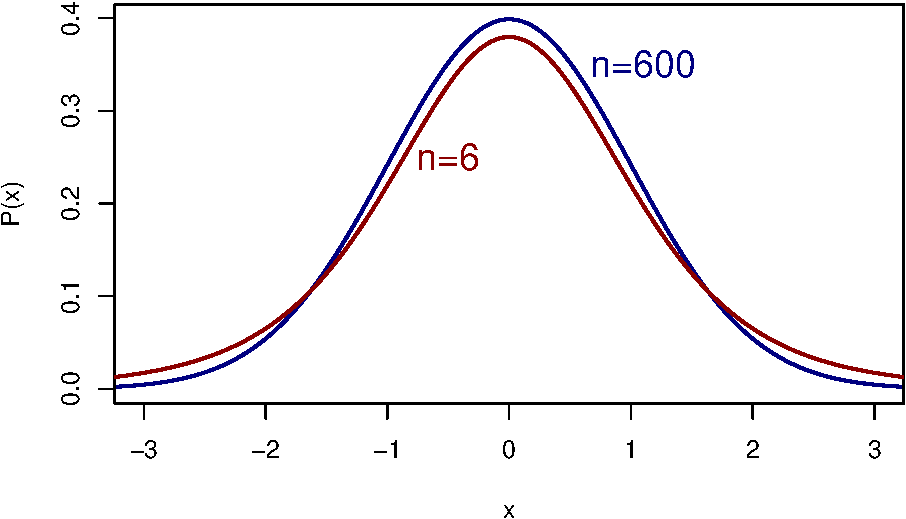
\includegraphics{KMS-NL_files/figure-latex/tkansverdeling-1.pdf}
\caption{\label{fig:tkansverdeling}Kansverdeling volgens de t-verdeling van een variabele \(x\) met gemiddelde 0 en standaarddeviatie 1, voor n=600 en n=6.}
\end{figure}

Voor de \(t\)-verdeling moeten we dus weten hoe groot de steekproef was;
deze \(n\) bepaalt immers de precieze kansverdeling van \(t\), en daarmee de
kritieke waarde \(t*\). We gaan daar nader op in in
§\ref{sec:ttoets-vrijheidsgraden}. We volstaan hier met een
uitgewerkt voorbeeld.

\begin{center}\rule{0.5\linewidth}{0.5pt}\end{center}

\begin{quote}
\emph{Voorbeeld 10.11:}
Soms wil een onderzoeker weten hoe snel het Nederlands eigenlijk
gesproken wordt, en hoe groot de variatie tussen sprekers is in deze
spreeksnelheid. Deze variabele, spreeksnelheid, wordt uitgedrukt als het
aantal seconden dat een lettergreep duurt (meestal \(<1\) seconde). Hoewel \citep{Quene08}
schat dat \(\mu=0.220\) s en \(\sigma=0.0225\) s, doen we alsof we deze
populatieparameters niet kennen --- net als echte onderzoekers, die deze
populatieparameters meestal ook niet kennen.
\end{quote}

\begin{quote}
Voor een steekproef van \(n=30\) sprekers vinden we \(\bar{x}=0.215\) en
\(s=0.0203\) seconden. Daaruit schatten\footnote{Schattingen van parameters worden aangegeven met een ``dakje'' erboven.} we \(\hat{\mu}=0.215\) en
\(\hat{\sigma}=0.0203\). Omdat \(\sigma\) niet bekend is, gebruiken we de
\(t\)-verdeling om het betrouwbaarheidsinterval te bepalen. We gebruiken
de \(t\)-verdeling voor \(n=30\) en vinden een kritieke waarde \(t^*=2.05\)
(zie
Bijlage \ref{app:kritieketwaarden}, voor \(B=95\)\%).
Volgens
formule \eqref{eq:t-onesampleCI} weten we dan met 95\% betrouwbaarheid dat het onbekende populatiegemiddelde \(\mu\) ligt tussen
\(\bar{x}-2.05\times s_{\bar{x}}\) en \(\bar{x}+2.05\times s_{\bar{x}}\),
oftewel tussen \(0.215-2.05\times0.0037\) en \(0.215+2.05\times0.0037\),
oftewel tussen \(0.208\) en \(0.223\) seconde.
\end{quote}

\begin{center}\rule{0.5\linewidth}{0.5pt}\end{center}

In Figuur \ref{fig:tempo95CIs} zie je de resultaten van een
computer-simulatie om dit te illustreren. We hebben \(100\times\)
denkbeeldige steekproeven getrokken van \(n=30\) moedertaalsprekers van
het Standaard Nederlands, en de spreeksnelheid vastgesteld van deze
sprekers. Voor elke steekproef hebben we het 95\%
betrouwbaarheidsinterval getekend. Voor 95 van de 100 steekproeven valt
het populatiegemiddelde \(\mu=0.220\) inderdaad binnen het interval, maar
voor 5 van de 100 steekproeven ten onrechte niet (deze zijn gemarkeerd
langs de rechterkant).

\begin{figure}
\centering
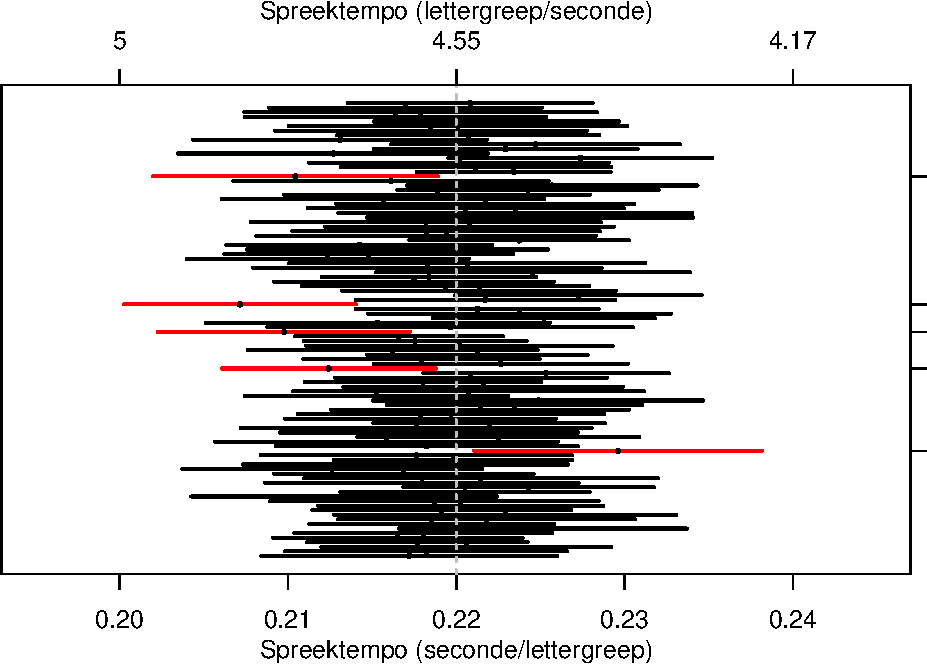
\includegraphics{KMS-NL_files/figure-latex/tempo95CIs-1.pdf}
\caption{\label{fig:tempo95CIs}95\%-Betrouwbaarheidsintervallen en steekproefgemiddelden, over 100 gesimuleerde steekproeven (n=30) uit een populatie met gemiddelde 0.220 en s.d. 0.0225; zie tekst.}
\end{figure}

\hypertarget{formules-2}{%
\subsection{formules}\label{formules-2}}

Het tweezijdige \(B\)\% betrouwbaarheidsinterval voor het
populatie-gemiddelde is
\begin{equation}
  \bar{X} \pm t^*_{n-1} \times \frac{s}{\sqrt{n}}
  \label{eq:t-onesampleCI}
\end{equation}
waarbij \(t^*\) met \(n-1\) vrijheidsgraden gevonden wordt met behulp van
Bijlage \ref{app:kritieketwaarden}, zie
§\ref{sec:ttoets-vrijheidsgraden} voor meer uitleg hierover.

\hypertarget{ch:samenhang}{%
\chapter{Samenhang}\label{ch:samenhang}}

\hypertarget{inleiding-5}{%
\section{Inleiding}\label{inleiding-5}}

Het meeste empirische onderzoek is gericht op het vaststellen van
samenhang tussen variabelen. In experimenteel onderzoek gaat het dan
primair om de samenhang tussen onafhankelijke en afhankelijke
variabelen. In het volgende deel gaan we nader in op diverse manieren om
vast te stellen of er een ``significant'' (beduidend, betekenisvol, niet
toevallig) verband bestaat tussen de onafhankelijke en afhankelijke
variabele. Daarnaast kan de onderzoeker geïnteresseerd zijn in de
onderlinge samenhang tussen meerdere afhankelijke variabelen,
bijvoorbeeld de samenhang tussen de oordelen van meerdere beoordelaars
(zie ook Hoofdstuk \ref{ch:betrouwbaarheid}).

In quasi-experimenteel onderzoek is het onderscheid tussen
onafhankelijke en afhankelijke variabelen doorgaans minder duidelijk. Er
worden meerdere variabelen geobserveerd, en de onderzoeker is vooral
geïnteresseerd in de onderlinge samenhang tussen die geobserveerde
variabelen. Wat is bijvoorbeeld de samenhang tussen de scores voor
lezen, rekenen, en wereldoriëntatie in het CITO-onderzoek (zie
Tabel \ref{tab:cito})? In dit hoofdstuk gaan we nader in op de manieren
om die samenhang of correlatie uit te drukken in een getal: een
correlatie-coëfficient. Afhankelijk van de meetniveau's van de
variabelen zijn er verschillende correlatie-coëfficiënten, die we verder
in dit hoofdstuk zullen behandelen.

Het is raadzaam om altijd eerst een grafische weergave te maken van de
samenhang tussen de variabelen, in de vorm van een zgn.
\emph{spreidingsdiagram} (ook vaak aangeduid als scattergram of scatterplot),
zoals in Figuur \ref{fig:cito-scatter}. Ieder punt in dit spreidingsdiagram
correspondeert met een leerling (of algemener, met een eenheid van de
steekproef). De positie van ieder punt (leerling) wordt bepaald door de
geobserveerde waarden van twee variabelen (hier is \(X\) score bij
leestoets, \(Y\) is score bij rekentoets). Zo'n spreidingsdiagram helpt om
een eventueel verband te interpreteren, en om te inspecteren of de
observaties wel voldoen aan de randvoorwaarden om een correlatie te
berekenen uit die observaties. Kijk in ieder geval naar (a) de
aanwezigheid van een eventueel verband, (b) de vorm van dat verband
(lineair, exponentieel, \ldots), (c) eventuele uitbijters (extreme
observaties, zie §\ref{sec:uitbijters}), en (d) de verdeling van de twee
variabelen, zie §\ref{sec:robuustefficient}.

\begin{figure}

{\centering 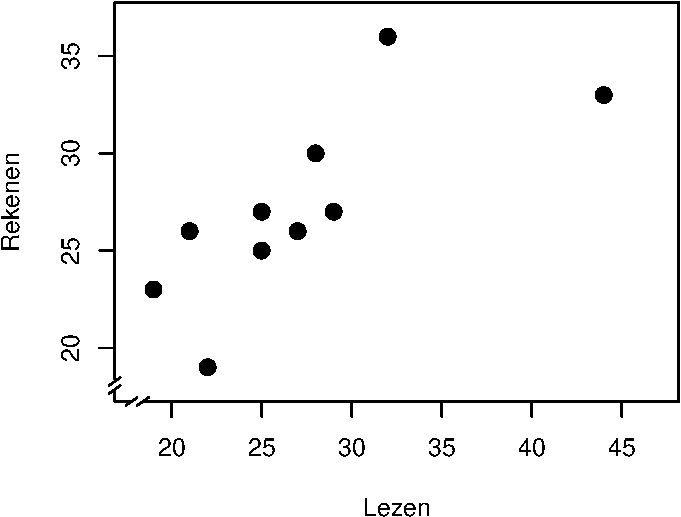
\includegraphics{KMS-NL_files/figure-latex/cito-scatter-1} 

}

\caption{Spreidingsdiagram van de scores van een leestoets en een rekentoets; zie tekst.}\label{fig:cito-scatter}
\end{figure}

Dit spreidingsdiagram laat zien (a) dat er een verband bestaat tussen de
scores bij lezen en bij rekenen. Het verband is (b) bij benadering lineair, d.w.z. te
beschrijven als een rechte lijn; we komen daar op terug in
§\ref{sec:regressie}.
Het verband helpt ons ook om de spreiding in de twee variabelen te
verklaren. Immers, de spreiding in de rekenscores is voor een deel te
begrijpen of te verklaren uit de spreiding in de leestoets: leerlingen
die een relatief goede score behalen bij lezen, doen dat ook bij
rekenen. De observaties van de twee variabelen verschaffen dus niet
alleen informatie over die twee variabelen zelf, maar bovendien over de
samenhang tussen die variabelen. In dit spreidingsdiagram zien we
overigens ook (c) dat de hoogste leesscore een uitbijter vormt (zie ook
Fig.\ref{fig:cito-boxplot}); zulke uitbijters kunnen onevenredig
grote invloed hebben op het gevonden verband.

\hypertarget{sec:Pearson}{%
\section{Pearson product-moment-correlatie}\label{sec:Pearson}}

De Pearson product-moment-correlatiecoëfficiënt wordt aangeduid met
symbool \(r\) (in het geval van twee variabelen). Deze coëfficiënt is te
gebruiken als beide variabelen geobserveerd zijn op het
interval-meetniveau
(§\ref{sec:interval}), en als beide variabelen bij benadering
normaal-verdeeld zijn
(§\ref{sec:normaalverdeling}). De berekening doen we tegenwoordig
per computer.

Voor de observaties in het spreidingsdiagram in
Fig.\ref{fig:cito-scatter} vinden we een correlatie van \(r=+.79\). De
correlatie-coëfficiënt is een getal dat per definitie ligt tussen \(-1\)
en \(+1\). Een positieve correlatiecoëfficient wijst op een positief
verband: een grotere waarde van \(X\) correspondeert met een grotere
waarde van \(Y\). Een negatieve coëfficiënt wijst op een negatief verband:
een grotere waarde van \(X\) correspondeert met een kleinere waarde van
\(Y\). Een waarde van \(r\) dicht bij nul wijst op een zwak of afwezig
verband: de spreiding in \(X\) heeft niets te maken met de spreiding in
\(Y\); er is geen of alleen zwakke correlatie. Een correlatie van
\(.4<r<.6\) (of \(-.6 < r < -.4\)) noemen we middelmatig. Een correlatie van
\(r>.6\) (of \(r< -.6\)) wijst op een sterke samenhang. Als \(r=1\) (of
\(r=-1\)) dan liggen alle observaties precies op een rechte lijn.
Figuur \ref{fig:cor-scatter} toont meerdere spreidingsdiagrammen met de
bijbehorende correlatiecoëfficiënten.

\begin{figure}

{\centering 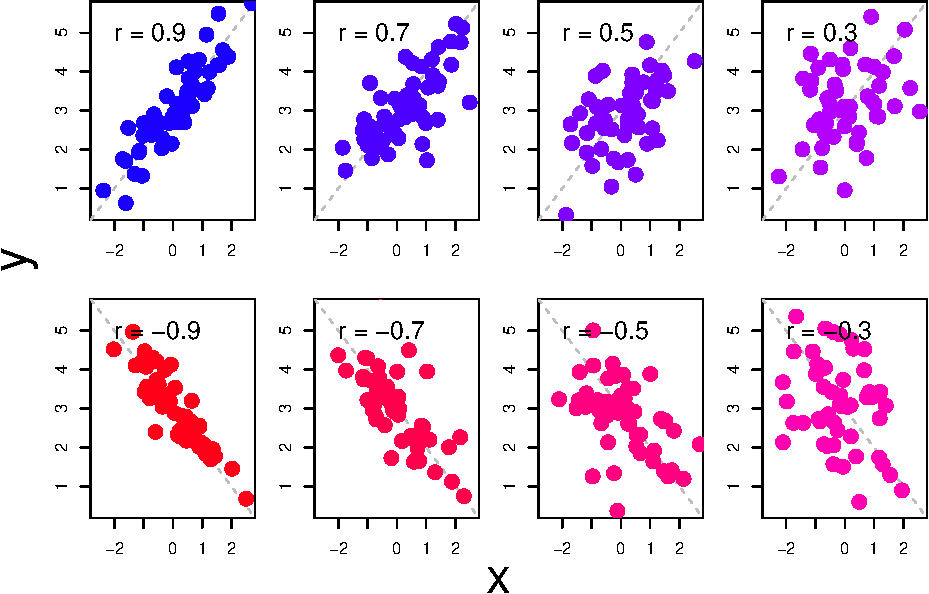
\includegraphics{KMS-NL_files/figure-latex/cor-scatter-1} 

}

\caption{Meerdere spreidingsdiagrammen van observaties met bijbehorende correlatiecoëfficiënten.}\label{fig:cor-scatter}
\end{figure}

De correlatie die we zien tussen de scores van de twee variabelen (zoals
\(r=.79\) tussen scores bij leestoets en rekentoets,
Fig.\ref{fig:cito-scatter}) zou ook het gevolg kunnen zijn van
toevallige variaties in de observaties. Het is immers mogelijk dat de
leerlingen met een goede score op de leestoets, zuiver door toeval, ook
een goede score op de rekentoets hebben behaald --- ook als er in de
populatie eigenlijk \emph{niet} samenhang is tussen de twee variabelen. De
onbekende correlatie in de populatie duiden we aan met de griekse letter
\(\rho\) (``rho''); het is dus ook mogelijk dat \(\rho=0\). Ook als \(\rho=0\)
is het mogelijk om \(n=10\) leerlingen in de steekproef te hebben die hoge
scores op het ene onderdeel \emph{toevallig} combineren met hoge scores op
het andere onderdeel (en om toevallig niet leerlingen in de steekproef
te hebben die hoge scores op het ene onderdeel combineren met lage
scores op het andere onderdeel). We kunnen schatten wat de kans \(p\) is
om deze correlatie van \(r=0.79\) of sterker te vinden in een steekproef
van \(n=10\) leerlingen, indien de samenhang in de populatie eigenlijk
nihil is (d.i. indien \(\rho=0\)). Deze kans \(p\) noemen we de
\emph{significantie} van de correlatiecoëfficiënt; we komen in
Hoofdstuk \ref{ch:toetsing} uitgebreider terug op dit begrip
`significantie'. Daarop vooruitlopend: als deze kans \(p\) kleiner is dan
\(.05\), dan nemen we aan dat de gevonden correlatie \(r\) \emph{niet toevallig},
d.i. \emph{significant} is. Vaak zien we een kleine kans \(p\) bij een sterke
correlatie \(r\). De correlatiecoëfficiënt \(r\) geeft de richting en
sterkte van het verband aan, en de significantie \(p\) geeft de kans aan
om dit verband bij toeval te vinden als \(\rho=0\) in de populatie. We
rapporteren deze bevindingen als volgt\footnote{Als de gevonden correlatie \(r\) \emph{niet} significant is, dan kan die dus ook toevallig zijn, en dan laten we een interpretatie van de samenhang dus achterwege. We vermelden in ons verslag dan wel de gevonden correlatiecoëfficiënt en de gevonden significantie daarvan.}:

\begin{center}\rule{0.5\linewidth}{0.5pt}\end{center}

\begin{quote}
\emph{Voorbeeld 11.1:}
De scores van de \(n=10\) leerlingen op de deeltoetsen van de CITO-toets
in Tabel \ref{tab:cito} laten een sterke correlatie zien tussen de scores
bij de onderdelen Lezen en Rekenen: Pearson \(r=0.79, p=.007\). Leerlingen
met een relatief hoge score bij het ene onderdeel behalen in het
algemeen ook een relatief hoge score bij het andere onderdeel.
\end{quote}

\begin{center}\rule{0.5\linewidth}{0.5pt}\end{center}

In veel onderzoeken zijn we geïnteresseerd in de correlaties tussen meer
dan twee variabelen. Die correlaties tussen variabelen worden dan vaak
gerapporteerd in een zgn. correlatiematrix zoals
Tabel \ref{tab:cito-correlaties}, dat is een tabel waar de correlaties
vermeld worden van alle paren van correlaties (Eng. `pairwise
correlation matrix').

\begin{longtable}[]{@{}lccc@{}}
\caption{\label{tab:cito-correlaties} Correlaties tussen de drie onderdelen van de CITO-toets, zoals
samengevat in Tabel \ref{tab:cito}, met bijbehorende significantie-niveau
tussen haakjes.}\tabularnewline
\toprule
& Lezen & Rekenen & Wereldoriëntatie\tabularnewline
\midrule
\endfirsthead
\toprule
& Lezen & Rekenen & Wereldoriëntatie\tabularnewline
\midrule
\endhead
Lezen & 1.00 & &\tabularnewline
Rekenen & 0.79 (.007) & 1.00 &\tabularnewline
Wereldoriëntatie & -0.51 (.131) & -0.01 (.970) & 1.00\tabularnewline
\bottomrule
\end{longtable}

In deze matrix is alleen de onderste (linker) helft van de volledige
matrix weergegeven. Dat is ook voldoende, want de cellen zijn gespiegeld
rond de diagonaal: de correlatie tussen Lezen (kolom 1) en Rekenen (rij
2) is immers hetzelfde als de correlatie tussen Rekenen (rij 2) en Lezen
(rij 1). De correlatiematrix bevat in de cellen op de diagonaal altijd
de waarde \(1.00\), omdat een variabele altijd perfect met zichzelf
correleert. We rapporteren deze bevindingen als volgt:

\begin{center}\rule{0.5\linewidth}{0.5pt}\end{center}

\begin{quote}
\emph{Voorbeeld 11.2:} De
paarsgewijze correlaties tussen scores van de \(n=10\) leerlingen op de
drie deeltoetsen van de CITO-toets zijn samengevat in
Tabel \ref{tab:cito-correlaties}. We zien een sterke correlatie tussen
de scores bij de onderdelen Lezen en Rekenen: leerlingen met een
relatief hoge score bij het onderdeel Lezen behalen in het algemeen ook
een relatief hoge score bij het onderdeel Rekenen. De overige
correlaties waren niet significant.
\end{quote}

\begin{center}\rule{0.5\linewidth}{0.5pt}\end{center}

\hypertarget{formules-3}{%
\subsection{Formules}\label{formules-3}}

De eenvoudigste formule voor de Pearson
product-moment-correlatiecoëfficiënt \(r\) maakt gebruik van de
standaard-normaal-scores die we al eerder gebruikt hebben
(§\ref{sec:standaardscores}):
\begin{equation}
    r_{XY} = \frac{\sum z_X z_Y}{n-1}
  \label{eq:pearson}
\end{equation}

Net als bij het berekenen van de variantie
(formule \eqref{eq:variantie}) delen we weer door \((n-1)\) om een schatting
te maken van de samenhang in de populatie.

\hypertarget{spss-5}{%
\subsection{SPSS}\label{spss-5}}

Voor Pearson's product-moment-correlatiecoëfficiënt:

\begin{verbatim}
Analyze > Correlate > Bivariate...
\end{verbatim}

Kies \texttt{Pearsons} correlatiecoëfficiënt, vink aan:
\texttt{Flag\ significant\ correlations}. Bevestig met \texttt{OK}. De resulterende
uitvoer (tabel) voldoet niet aan de stijl-eisen; je moet de gegevens dus
overnemen in of omzetten naar een eigen tabel die daar wel aan voldoet.

\hypertarget{r-6}{%
\subsection{R}\label{r-6}}

\begin{Shaded}
\begin{Highlighting}[]
\NormalTok{cito \textless{}{-}}\StringTok{ }\KeywordTok{read.table}\NormalTok{(}\DataTypeTok{file=}\StringTok{"data/cito.txt"}\NormalTok{, }\DataTypeTok{header=}\OtherTok{TRUE}\NormalTok{)}
\KeywordTok{cor}\NormalTok{( cito[,}\DecValTok{2}\OperatorTok{:}\DecValTok{4}\NormalTok{] ) }\CommentTok{\# correlatie{-}matrix van kolommen 2,3,4}
\end{Highlighting}
\end{Shaded}

\begin{verbatim}
##                       Lezen    Rekenen Wereldoriëntatie
## Lezen             1.0000000 0.74921033      -0.50881738
## Rekenen           0.7492103 1.00000000       0.06351024
## Wereldoriëntatie -0.5088174 0.06351024       1.00000000
\end{verbatim}

\begin{Shaded}
\begin{Highlighting}[]
\KeywordTok{with}\NormalTok{( cito, }\KeywordTok{cor.test}\NormalTok{( Lezen, Rekenen ) )}
\end{Highlighting}
\end{Shaded}

\begin{verbatim}
## 
##  Pearson's product-moment correlation
## 
## data:  Lezen and Rekenen
## t = 3.1994, df = 8, p-value = 0.01262
## alternative hypothesis: true correlation is not equal to 0
## 95 percent confidence interval:
##  0.2263659 0.9368863
## sample estimates:
##       cor 
## 0.7492103
\end{verbatim}

\hypertarget{sec:regressie}{%
\section{Regressie}\label{sec:regressie}}

Het meest eenvoudige verband dat we kunnen onderscheiden en beschrijven
is een lineair verband, d.w.z. een rechte lijn in het spreidingsdiagram
(zie Fig.\ref{fig:cor-scatter}). Deze rechte lijn geeft aan welke waarde
van \(Y_i\) voorspeld wordt, op basis van de waarde van \(X_i\). Deze
voorspelde waarde van \(Y_i\) wordt genoteerd als \(\widehat{Y_i}\)
(``Y-hat''). De beste voorspelling \(\widehat{Y_i}\) is gebaseerd op de
waarde van \(X_i\) èn op het lineaire verband tussen \(X\) en \(Y\):
\begin{equation}
    \widehat{Y_i} = a + b {X_i} 
  \label{eq:linearmodel2}
\end{equation}\\
De rechte lijn wordt beschreven met
twee parameters, nl. het begingetal \(a\) (Eng. `intercept') en de
hellingscoëfficiënt \(b\) (Eng. `slope')\footnote{In schoolboeken wordt deze vergelijking ook wel beschreven als \(Y = a X + b\), met \(a\) als hellingscoëfficiënt en \(b\) als begingetal; we houden ons hier echter aan de internationaal gangbare notatie.}. De rechte lijn die het
lineaire verband beschrijft wordt ook aangeduid als de ``regressielijn'';
we proberen immers om de geobserveerde waarden van \(Y\) te herleiden tot
deze lineaire functie van de waarden van \(X\).

Het verschil tussen de geobserveerde waarde \(Y\) en de voorspelde waarde
\(\widehat{Y}\) \((Y-\widehat{Y})\) wordt het \emph{residu} genoemd (symbool
\(e\)). Anders gezegd, de geobserveerde waarde wordt beschouwd als de
optelsom van twee componenten, nl. de voorspelde waarde en het residu:
\begin{align}
    Y   &= \widehat{Y} + e \\
        &= a + b X + e 
  \label{eq:linearmodel3}
\end{align}

Bovenstaande gedachtengang wordt geïllusteerd in het spreidingsdiagram
in Figuur \ref{fig:cito-linearmodel}. De stippellijn geeft het lineaire
verband aan tussen de twee toetsen:
\begin{equation}
    \widehat{\textrm{Rekenen}} = 12.97 + 0.52 \times \textrm{Lezen}
  \label{eq:cito-linearmodel}
\end{equation}

\begin{figure}

{\centering 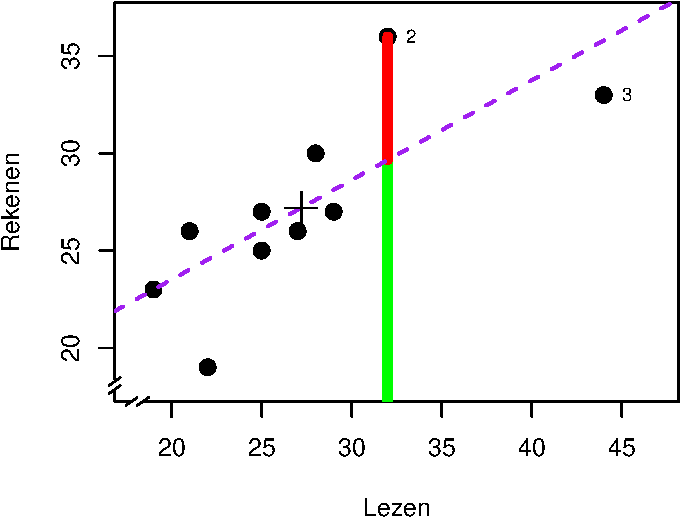
\includegraphics{KMS-NL_files/figure-latex/cito-linearmodel-1} 

}

\caption{Spreidingsdiagram van de scores van een leestoets en een rekentoets. In het diagram is tevens aangegeven de regressielijn (stippellijn), de voorspelde waarde (groen) en residu (rood) van de rekentoets voor leerling 2, de gemiddelden (plus-symbool), en markeringen voor leerling 2 en 3; zie tekst.}\label{fig:cito-linearmodel}
\end{figure}

Deze stippellijn geeft dus aan wat de voorspelde waarde \(\widehat{Y}\) is
voor iedere waarde van \(X\). Voor de tweede leerling met \(X_2 = 32\)
voorspellen we zo \(\widehat{Y_2} = 12.97 + (0.52) (32) = 29.61\)
(voorspelde waarde, groene lijnstuk). Voor alle observaties die niet
precies op deze regressielijn liggen (stippellijn),
is er een afwijking tussen de voorspelde
score \(\widehat{Y}\) en de geobserveerde score \(Y\) (residu, rode
lijnstuk). Voor de tweede leerling is deze afwijking
\(e_2 = (Y_2 - \widehat{Y_2}) = (36-29.61) = 6.49\) (residu, rode
lijnstuk).

Zoals gezegd worden de geobserveerde waarden van \(Y\) beschouwd als de
optelsom van twee componenten, de voorspelde waarde \(\widehat{Y}\)
(groen) en het residu \(e\) (rood). Op dezelfde wijze kan ook de totale
\emph{variantie} van \(Y\) beschouwd worden als de optelsom van de twee
\emph{varianties} van deze componenten:
\begin{equation}
    s^2_{Y} = s^2_{\widehat{Y}} + s^2_e
  \label{eq:variance-pred-res}
\end{equation}
Van de totale variantie
\(s^2_Y\) van Y is dus het ene deel (\(s^2_{\widehat{Y}}\)) te herleiden tot
c.q. te verklaren uit de variantie van \(X\), via het lineaire verband
beschreven met parameters \(a\) en \(b\) (zie
formule \eqref{eq:linearmodel2}), en het andere deel (\(s^2_e\)) is niet te
herleiden of te verklaren. Dat tweede deel, de niet-voorspelde variantie
van de residuen, wordt ook wel de `residuele variantie' of `ruis'
genoemd.

Als we \(Y\) goed kunnen voorspellen uit \(X\), d.w.z. als de Pearson
product-moment-correlatiecoëfficiënt \(r\) hoog is
(Fig. \ref{fig:cor-scatter}, links), dan zijn de residuen \(e\) dus
relatief klein, de observaties liggen dicht rond de regressielijn in het
spreidingsdiagram, en dan is dus ook de residuele variantie \(s^2_e\)
relatief gering. Omgekeerd, als we \(Y\) \emph{niet} goed kunnen voorspellen
uit \(X\), d.w.z. als de correlatiecoëfficiënt \(r\) relatief laag is
(Fig. \ref{fig:cor-scatter}, rechts), dan zijn de residuen \(e\) dus
relatief groot, de observaties liggen wijd verspreid rond de
regressielijn in het spreidingsdiagram, en dan is dus ook de residuele
variantie \(s^2_e\) relatief groot. Het kwadraat van de Pearson
product-moment-correlatiecoëfficiënt \(r\) geeft aan wat de relatieve
omvang is van de twee variantie-componenten, ten opzichte van de totale
variantie:
\begin{align}
    r^2 & = \frac{s^2_{\widehat{Y}}}{s^2_Y} \\
        & = 1 - \frac{s^2_e}{s^2_Y}
  \label{eq:r2}
\end{align}
Deze grootheid \(r^2\) wordt ook wel aangeduid als de
``proportie verklaarde variantie'' of als de ``determinatie-coëfficiënt''.

De waarden van de lineaire parameters \(a\) en \(b\) in
formule \eqref{eq:linearmodel2} worden zo gekozen dat de verzamelde
residuen zo klein mogelijk zijn, d.w.z. dat de residuele variantie
\(s^2_e\) zo klein mogelijk is (``least squares fit''), en dus \(r^2\) zo
groot mogelijk (zie
§\ref{sec:regressie-formules}). Op die manier vinden we een rechte
lijn die het beste past bij de observaties van \(X\) en \(Y\).

Een lineaire regressie kan worden gerapporteerd als volgt:

\begin{center}\rule{0.5\linewidth}{0.5pt}\end{center}

\begin{quote}
\emph{Voorbeeld 11.3:}
Uit een lineaire-regressie-analyse blijkt dat de score bij Rekenen
samenhangt met die bij Lezen: \(b=0.51, r=.79, p_r=.007\), over \(n=10\)
leerlingen. Dit lineaire regressiemodel verklaart \(r^2=.51\) van de
totale variantie in de rekenscores (de residuele standaarddeviatie is
\(s_e= \sqrt{82.803/(n-1-1)} = 3.217\)).
\end{quote}

\begin{center}\rule{0.5\linewidth}{0.5pt}\end{center}

\hypertarget{sec:regressie-formules}{%
\subsection{Formules}\label{sec:regressie-formules}}

Bij lineaire regressie van \(y\) op \(x\) proberen we de coëfficiënten \(a\)
en \(b\) zodanig te schatten dat (het kwadraat van) de afwijking tussen de
voorspelde waarde \(\hat{y}\) en de geobserveerde waarde \(y\) zo klein
mogelijk is, m.a.w. dat het kwadraat van de residuen \((y-\hat{y})\) zo
klein mogelijk is. Dit wordt de ``least squares'' methode genoemd (zie
\url{http://www.itl.nist.gov/div898/handbook/pmd/section4/pmd431.htm}).

De beste schatting voor \(b\) is
\[b = \frac{ \sum_{i=1}^n (x_i-\overline{x})(y_i-\overline{y}) } { \sum_{i=1}^n (x_i-\overline{x})^2 }\]

De beste schatting voor \(a\) is \[a = \overline{y} - b \overline{x}\]

\hypertarget{spss-6}{%
\subsection{SPSS}\label{spss-6}}

Voor lineaire regressie:

\begin{verbatim}
Analyze > Regression > Linear...
\end{verbatim}

Kies \texttt{Dependent\ variable:\ Rekenen} en kies
\texttt{Independent\ variable:\ Lezen}. Onder de knop \texttt{Statistics}, vink aan
\texttt{Model\ fit}, vink aan \texttt{R\ squared\ change}, kies \texttt{Estimates}, en daarna
\texttt{Continue}.\\
Onder de knop \texttt{Plot}, vink aan \texttt{Histogram} en vink ook aan
\texttt{Normal\ probability\ plot}; deze keuzes zijn vereist om een numerieke(!)
samenvatting te krijgen over de residuals.\\
Onder de knop \texttt{Options}, kies \texttt{Include\ constant} om ook de constante
coëfficiënt \(a\) te laten berekenen. Bevestig alle keuzes met \texttt{OK}.

De resulterende uitvoer omvat meerdere tabellen en figuren; deze kan je
niet rechtstreeks overnemen in je verslag. De tabel getiteld \emph{Model
Summary} bevat de correlatie-coëfficiënt, hier aangeduid met hoofdletter
\(R=.749\).\\
De tabel getiteld \emph{Coefficients} bevat de regressie-coëfficienten. De
regel met aanduiding \texttt{(Constant)} vermeldt coëfficient \(a=13.25\); de
regel getiteld \texttt{Lezen} vermeldt coëfficient \(b=0.51\).\\
De tabel getiteld \emph{Residual Statistics} geeft informatie over zowel de
voorspelde waarden als de residuen. Controleer of het gemiddelde van de
residuen inderdaad nul is. In deze tabel zien we ook (regel 2, kolom 4)
dat de standaarddeviatie van de residuen \(3.212\) is.

\hypertarget{r-7}{%
\subsection{R}\label{r-7}}

\begin{Shaded}
\begin{Highlighting}[]
\KeywordTok{summary}\NormalTok{( m1 \textless{}{-}}\StringTok{ }\KeywordTok{lm}\NormalTok{( Rekenen}\OperatorTok{\textasciitilde{}}\NormalTok{Lezen, }\DataTypeTok{data=}\NormalTok{cito ) )}
\end{Highlighting}
\end{Shaded}

\begin{verbatim}
## 
## Call:
## lm(formula = Rekenen ~ Lezen, data = cito)
## 
## Residuals:
##     Min      1Q  Median      3Q     Max 
## -5.5332 -1.1167 -0.5332  1.7168  6.3384 
## 
## Coefficients:
##             Estimate Std. Error t value Pr(>|t|)  
## (Intercept)  13.2507     4.4910   2.950   0.0184 *
## Lezen         0.5128     0.1603   3.199   0.0126 *
## ---
## Signif. codes:  0 '***' 0.001 '**' 0.01 '*' 0.05 '.' 0.1 ' ' 1
## 
## Residual standard error: 3.406 on 8 degrees of freedom
## Multiple R-squared:  0.5613, Adjusted R-squared:  0.5065 
## F-statistic: 10.24 on 1 and 8 DF,  p-value: 0.01262
\end{verbatim}

Het command \texttt{lm} specificeert een lineair regressiemodel, met \texttt{Rekenen}
als afhankelijke variabele en \texttt{Lezen} als predictor. Dit model wordt
bewaard als een object genaamd \texttt{m1}, en dat wordt meteen weer gebruikt
als argument (invoer) om te rapporteren. In die rapportage van model
\texttt{m1} wordt de constante coëfficient \(a\) aangeduid als \texttt{Intercept}.

\begin{Shaded}
\begin{Highlighting}[]
\KeywordTok{sd}\NormalTok{( }\KeywordTok{resid}\NormalTok{( m1 ) ) }\CommentTok{\# s.d. van residuen volgens \textasciigrave{}m1\textasciigrave{}}
\end{Highlighting}
\end{Shaded}

\begin{verbatim}
## [1] 3.211533
\end{verbatim}

\hypertarget{invloedrijke-observaties}{%
\section{Invloedrijke observaties}\label{invloedrijke-observaties}}

In de vorige paragraaf zagen we dat in een correlatie-analyse of een
regressie-analyse gestreefd wordt naar een minimale residuele variantie.
Eerder zagen we al ook dat uitbijters of extreme observaties, per
definitie, relatief veel bijdragen aan de variantie. Bij elkaar leidt
dat ertoe, dat uitbijters of extreme observatie grote invloed kunnen
hebben op de hoogte van de correlatie, of op de gevonden regressie (het
gevonden lineaire verband). Dat is ook te zien in
Fig.\ref{fig:cito-linearmodel}. Leerling 3 heeft een extreem hoge
score bij Lezen (zie ook
Fig.\ref{fig:cito-boxplot}). Als we deze leerling 3 buiten
beschouwing laten dan zou er niet veel veranderen aan de correlatie
(\(r_{-3}=.79\)) maar wel aan de helling van de regressielijn (\(b=0.84\),
ruim anderhalf keer zo groot als mèt leerling 3). Deze observatie
``trekt'' dus hard aan de regressielijn, juist omdat deze observatie een
extreme waarde heeft voor \(X\) en daardoor veel invloed heeft.

Ook niet-extreme observaties kunnen toch van grote invloed zijn op de
correlatie en regressie, als ze ver verwijderd zijn van de regressielijn
en dus een grote bijdrage leveren aan de residuele variantie. Ook dat is
te zien in Fig.\ref{fig:cito-linearmodel}.
Leerling 2 heeft geen extreme scores,
maar heeft wel het grootste residu. Als we deze leerling 2 buiten
beschouwing laten dan zou de correlatie aanzienlijk hoger zijn
(\(r_{-2}=.86\)) maar de helling van de regressielijn zou slechts weinig
veranderen (\(b=0.45\)).

Bij een correlatie-analyse of regressie-analyse moet je daarom altijd
een spreidingsdiagram maken en bestuderen, om te kijken in hoeverre de
resultaten beïnvloed zijn door een of enkele observaties. Let daarbij
speciaal op observaties die ver verwijderd zijn van het gemiddelde, voor
elk van beide variabelen, en op observaties die ver verwijderd zijn van
de regressielijn.

\hypertarget{sec:Spearman}{%
\section{Spearmans rangorde-correlatie}\label{sec:Spearman}}

De beide variabelen waarvan we de correlatie willen onderzoeken, zijn
niet altijd uitgedrukt op het interval-meetniveau
(§\ref{sec:interval}), of de onderzoekers willen of kunnen niet aannemen dat
de beide variabelen bij benadering normaal-verdeeld zijn
(§\ref{sec:normaalverdeling}).
In dat geval is de
product-moment-correlatie minder geschikt om de samenhang te
kwantificeren. Indien de gegevens wel op ordinaal meetniveau zijn
uitgedrukt, dan kunnen we wel andere correlatiecoëfficiënten gebruiken
om de samenhang uit te drukken: Spearmans rangorde-correlatiecoëfficiënt
(\(r_s\)) en Kendalls \(\tau\) (de griekse letter ``tau''). Deze beide
coëfficiënten zijn gebaseerd op de rangordening van de observaties; deze
correlaties kunnen we dus altijd uitrekenen als we de observaties kunnen
ordenen. Ook deze berekening doen we tegenwoordig per computer. In dit
hoofdstuk bespreken we alleen de Spearmans
rangorde-correlatiecoëfficiënt.

De Spearman rangorde-correlatiecoëfficiënt is gelijk aan de Pearson
product-moment-correlatiecoëfficiënt toegepast op de \emph{rangnummers} van de
observaties. We zetten iedere observatie van een variabele om naar het
volgorde-nummer, van de kleinste geobserveerde waarde (volgnummer 1)
naar de grootste geobserveerde waarde (volgnummer \(n\)). Als twee of meer
observaties dezelfde waarde hebben, dan krijgen ze ook hetzelfde
(gemiddelde) rangnummer. In
Tabel \ref{tab:cito-rangnummers} zie je de rangnummers van de scores
voor Lezen en Rekenen, hier geordend volgens de rangnummers voor Lezen.

\begin{longtable}[]{@{}lcccccccccc@{}}
\caption{\label{tab:cito-rangnummers} Rangnummers van de scores van 10 leerlingen op onderdelen van een toets, zoals samengevat in Tabel \ref{tab:cito}, met verschil \(v_i\) tussen de twee rangnummers per leerling.}\tabularnewline
\toprule
Leerling & 1 & 9 & 6 & 4 & 10 & 8 & 5 & 7 & 2 & 3\tabularnewline
\midrule
\endfirsthead
\toprule
Leerling & 1 & 9 & 6 & 4 & 10 & 8 & 5 & 7 & 2 & 3\tabularnewline
\midrule
\endhead
Lezen & 1 & 2 & 3 & 4.5 & 4.5 & 6 & 7 & 8 & 9 & 10\tabularnewline
Rekenen & 2 & 4 & 1 & 4 & 6.5 & 4 & 8 & 6.5 & 10 & 9\tabularnewline
verschil \(v_i\) & -1 & -2 & 1 & 0.5 & -2 & 2 & -1 & 1.5 & -1 & 1\tabularnewline
\bottomrule
\end{longtable}

De ordening in Tabel \ref{tab:cito-rangnummers} maakt in één oogopslag duidelijk dat
de drie leerlingen met de laagste score voor Lezen (nrs. 1, 9, 6) ook
bijna de laagste scores voor Rekenen behaalden. Dat wijst op een
positief verband. De twee beste lezers (nrs. 2 en 3) zijn ook de twee
beste rekenaars. Ook dat wijst op een positief verband. Er is echter
geen sprake van een perfect positief verband (dus hier \(r_s<1\)), want
dan zouden de beide rangordeningen perfect overeen komen.

Bedenk zelf hoe Tabel \ref{tab:cito-rangnummers} er uit zou zien, als er een perfect
negatief verband zou zijn (\(r_s=-1\)) tussen de scores bij Lezen en
Rekenen, en hoe de tabel er uit zou zien als er geen enkel verband zou
zijn (\(r_s=0\)) tussen deze scores.

\hypertarget{formules-4}{%
\subsection{Formules}\label{formules-4}}

De samenhang tussen de rangnummers van twee variabelen wordt uitgedrukt
in de Spearman rangorde-correlatiecoëfficiënt:
\begin{equation}
    r_s = 1 - \frac{6 \sum v_i^2}{n(n^2-1)}
  \label{eq:spearman}
\end{equation}
waarin \(v_i\) staat voor
het verschil in rangnummers op beide variabelen voor respondent \(i\). De
breuk in deze formule wordt groter, en \(r_s\) wordt dus kleiner, naarmate
de verschillen tussen de rangnummers groter zijn.
Deze formule is echter alleen bruikbaar als er geen ``ties'' (gedeelde rangnummers) zijn in de variabelen; voor de gegevens in Tabel \ref{tab:cito-rangnummers} met ``ties'' in beide variabelen moeten we een andere formule gebruiken.

Zoals blijkt is de Spearmans rangorde-correlatie \(r_s\) niet gelijk aan
de Pearson product-momentcorrelatie \(r\) bij deze geobserveerde scores.
Indien voldaan wordt aan de voorwaarden voor de Pearson coëfficient, dan
geeft deze Pearson product-moment-correlatiecoëfficiënt een betere
schatting van de samenhang dan de Spearman
rangorde-correlatiecoëfficiënt. Maar als er \emph{niet} aan die voorwaarden
voldaan wordt, dan is de Spearman coëfficiënt weer te prefereren. De
Spearman coëfficiënt is onder andere minder gevoelig voor invloedrijke
extreme observaties --- dergelijke uitschieters leggen immers minder
gewicht in de schaal, nadat we de ruwe scores vervangen hebben door de
rangnummers.

\hypertarget{spss-7}{%
\subsection{SPSS}\label{spss-7}}

Voor Spearmans rangorde-correlatiecoëfficiënt:

\begin{verbatim}
Analyze > Correlate > Bivariate...
\end{verbatim}

Kies \texttt{Spearman} rangorde-correlatiecoëfficiënt, vink aan:
\texttt{Flag\ significant\ correlations}. Bevestig met \texttt{OK}. De resulterende
uitvoer (tabel) voldoet niet aan de stijl-eisen; je moet de gegevens dus
overnemen in of omzetten naar een eigen tabel die daar wel aan voldoet,
en rapporteren volgens de gebruikelijke conventies voor
correlatie-analyse.

\hypertarget{r-8}{%
\subsection{R}\label{r-8}}

\begin{Shaded}
\begin{Highlighting}[]
\KeywordTok{with}\NormalTok{(cito, }\KeywordTok{cor.test}\NormalTok{( Lezen,Rekenen, }\DataTypeTok{method=}\StringTok{"spearman"}\NormalTok{ ) )}
\end{Highlighting}
\end{Shaded}

\begin{verbatim}
## Warning in cor.test.default(Lezen, Rekenen, method = "spearman"): Cannot compute
## exact p-value with ties
\end{verbatim}

\begin{verbatim}
## 
##  Spearman's rank correlation rho
## 
## data:  Lezen and Rekenen
## S = 25.229, p-value = 0.00198
## alternative hypothesis: true rho is not equal to 0
## sample estimates:
##       rho 
## 0.8470988
\end{verbatim}

\hypertarget{sec:Phi}{%
\section{Phi}\label{sec:Phi}}

De beide variabelen waarvan we de samenhang willen onderzoeken, zijn
zelfs niet altijd uitgedrukt op het ordinale meetniveau
(Hoofdstuk \ref{ch:Meetniveau}). Zelfs als beide variabelen alleen op
nominaal niveau gemeten zijn, dan kan er nog een correlatie berekend
worden, nl. de phi-correlatiecoëfficiënt (symbool \(r_\Phi\), met griekse
letter ``Phi''). Deze correlatiecoëfficiënt is ook bruikbaar als één van
de twee variabelen op nominaal niveau gemeten is, en de andere op
ordinaal niveau.

Laten we bij ons voorbeeld met de CITO-toets aannemen dat de eerste vijf
leerlingen uit een grote stad komen, en de laatste vijf van het
platteland. De herkomst van de leerling vormt een nominale variabele,
met 2 categorieën, hier willekeurig aangeduid als \texttt{1} resp. \texttt{0} (zie
§\ref{sec:nominaal}; een nominale variabele met precies 2
categorieën wordt ook een binomiale of dichotome variabele genoemd). We
vragen ons nu af of er enige samenhang is tussen de herkomst van een
leerling en de score bij het onderdeel Rekenen van de CITO-toets. De
tweede variabele is van interval-niveau. We zetten deze om naar een
nominaal meetniveau. Dat kan op vele manieren, en het is aan de
onderzoeker om daarbij een verstandige keuze te maken. Wij kiezen hier
voor de vaak gebruikte `mean split': de ene categorie (laag, code \texttt{0})
bestaat uit scores kleiner dan of gelijk aan het gemiddelde
(§\ref{sec:gemiddelde}), en de andere categorie uit scores groter
dan het gemiddelde (hoog, code \texttt{1}). De aantallen leerlingen in elk van
de \(2\times 2\) categorieën vatten we samen in een kruistabel
(Tabel \ref{tab:cito-kruis}).

\begin{longtable}[]{@{}lccc@{}}
\caption{\label{tab:cito-kruis} Kruistabel van \(n=10\) leerlingen, onderverdeeld naar herkomst
(stad=1, platteland=0) en naar categorie van score bij het onderdeel Rekenen van een
CITO-toets (`mean split', laag=0, hoog=1), met letter-aanduiding voor de aantallen
observaties; zie tekst.}\tabularnewline
\toprule
herkomst & laag (0) & hoog (1) & totaal\tabularnewline
\midrule
\endfirsthead
\toprule
herkomst & laag (0) & hoog (1) & totaal\tabularnewline
\midrule
\endhead
platteland (0) & 5 (A) & 0 (B) & 5 (A+B)\tabularnewline
stad (1) & 2 (C) & 3 (D) & 5 (C+D)\tabularnewline
totaal & 7 (A+C) & 3 (B+D) & 10 (A+B+C+D)\tabularnewline
\bottomrule
\end{longtable}

De nominale correlatiecoëfficiënt \(r_\Phi\) is gelijk aan de Pearson
product-moment-correlatiecoëfficiënt als we die zouden toepassen op de binomiale codes
(\texttt{0} en \texttt{1}) van de observaties. Alle 5 de leerlingen van het platteland
hebben een score bij Rekenen gelijk aan of lager dan gemiddeld
(\(\overline{y}=\) 27.2); van de leerlingen uit de stad hebben er 2 een score
(gelijk aan of) lager dan gemiddeld. Er is dus samenhang tussen de
binomiale codes van de rijen (herkomst) en die van de kolommen
(score-categorieën) in Tabel \ref{tab:cito-kruis}.
Die samenhang wordt gekwantificeerd in de
correlatiecoëfficiënt \(r_\Phi=0.65\) voor deze gegevens.

\hypertarget{formules-5}{%
\subsection{Formules}\label{formules-5}}

De nominale correlatiecoëfficiënt \(r_\Phi\) wordt berekend als volgt,
waarbij de letters verwijzen naar de aantallen in de cellen van een
kruistabel (zie Tabel \ref{tab:cito-kruis}):
\begin{equation}
    r_\Phi = \frac{(AD-BC)}{\sqrt{(A+B)(C+D)(A+C)(B+D)}}
  \label{eq:phi}
\end{equation}

Voor het hierboven besproken voorbeeld vinden we dan
\[
    r_\Phi = \frac{(15-0)}{\sqrt{(5)(5)(7)(3)}} = \frac{15}{22.91} = 0.65
\]

\hypertarget{spss-8}{%
\subsection{SPSS}\label{spss-8}}

De dataset \texttt{cito} bevat al een variabele \texttt{StadPlat} die de herkomst van de leerlingen aangeeft. Maar volledigheidshalve leggen we toch uit hoe je zo'n variabele zelf kunt construeren.

\begin{verbatim}
Transform > Recode into different variables...
\end{verbatim}

Kies \texttt{Leerling} als oude variabele en vul als nieuwe naam \texttt{StadPlat2}
in voor de nieuwe variabele. Geef aan dat de oude waarden in \texttt{Range} van
1 t/m 5 (oud) omgezet moeten worden naar de nieuwe waarde 1, en evenzo
dat leerlingen 6 t/m 10 de nieuwe waarde 0 moeten krijgen voor de nieuwe
variabele \texttt{StadPlat}.

Voor \texttt{Rekenen} is het wat ingewikkelder. Je moet eerst je eerdere
omzettingsregels verwijderen (die betrekking hadden op \texttt{StadPlat}). Maak
dan op dezelfde wijze weer een nieuwe variabele, genaamd \texttt{Rekenen2}.
Alle waarden vanaf de laagste waarde tot het gemiddelde (\(27.2\)) worden
omgezet naar nieuwe waarde 0 voor die nieuwe variabele. Alle waarden
vanaf het gemiddelde (\(27.2\)) tot de hoogste waarde worden omgezet naar
nieuwe waarde 1.

Na dit voorbereidend werk kunnen we eindelijk \(r_\Phi\) gaan berekenen.

\begin{verbatim}
Analyze > Descriptives > Crosstabs...
\end{verbatim}

Selecteer de variabelen \texttt{StadPlat2} (in ``Rows'' paneel) en \texttt{Reken2}
(in ``Columns'' paneel) voor
kruistabel \ref{tab:cito-kruis}.\\
Kies \texttt{Statistics\ldots{}} en vink optie \texttt{Phi\ and\ Cramer’s\ V}aan!\\
Bevestig eerst met \texttt{Continue} en daarna nogmaals met \texttt{OK}.

\hypertarget{r-9}{%
\subsection{R}\label{r-9}}

De dataset \texttt{cito} bevat al een variabele StadPlat die de herkomst van de leerlingen aangeeft. Maar volledigheidshalve laten we toch zien hoe je zo'n variabele zelf kunt construeren.

\begin{Shaded}
\begin{Highlighting}[]
\NormalTok{StadPlat2 \textless{}{-}}\StringTok{ }\KeywordTok{ifelse}\NormalTok{( cito}\OperatorTok{$}\NormalTok{Leerling}\OperatorTok{\textless{}}\DecValTok{6}\NormalTok{, }\DecValTok{1}\NormalTok{, }\DecValTok{0}\NormalTok{) }\CommentTok{\# 1=stad, 0=plat}
\NormalTok{Reken2 \textless{}{-}}\StringTok{ }\KeywordTok{ifelse}\NormalTok{( cito}\OperatorTok{$}\NormalTok{Rekenen}\OperatorTok{\textgreater{}}\KeywordTok{mean}\NormalTok{(cito}\OperatorTok{$}\NormalTok{Rekenen), }\DecValTok{1}\NormalTok{, }\DecValTok{0}\NormalTok{ ) }\CommentTok{\# 1=hoog, 0=laag}
\end{Highlighting}
\end{Shaded}

Maak een nieuwe variabele \texttt{Reken2}, met de waarde 1 indien de score
voor Rekenen groter is dan het gemiddelde, en anders de waarde 0.

Ook in R maken we eerst een kruistabel (Tabel \ref{tab:cito-kruis}) en daarna berekenen we de \(r_\Phi\) over die kruistabel.

\begin{Shaded}
\begin{Highlighting}[]
\KeywordTok{print}\NormalTok{( }\KeywordTok{table}\NormalTok{(StadPlat2,Reken2) {-}\textgreater{}}\StringTok{ }\NormalTok{citokruistabel ) }\CommentTok{\# maak en bewaar en toon kruistabel}
\end{Highlighting}
\end{Shaded}

\begin{verbatim}
##          Reken2
## StadPlat2 0 1
##         0 5 0
##         1 2 3
\end{verbatim}

\begin{Shaded}
\begin{Highlighting}[]
\ControlFlowTok{if}\NormalTok{ (}\KeywordTok{require}\NormalTok{(psych)) \{ }\CommentTok{\# voor psych::phi}
  \KeywordTok{phi}\NormalTok{(citokruistabel) }\CommentTok{\# eerder gemaakte kruistabel is hier invoer!}
\NormalTok{\}}
\end{Highlighting}
\end{Shaded}

\begin{verbatim}
## Loading required package: psych
\end{verbatim}

\begin{verbatim}
## 
## Attaching package: 'psych'
\end{verbatim}

\begin{verbatim}
## The following objects are masked from '.hqenv':
## 
##     harmonic.mean, logit
\end{verbatim}

\begin{verbatim}
## [1] 0.65
\end{verbatim}

\hypertarget{sec:correlationcausation}{%
\section{Tenslotte}\label{sec:correlationcausation}}

Bij het einde van dit hoofdstuk willen we nog eens benadrukken dat een
samenhang of correlatie tussen twee variabelen niet noodzakelijkerwijs
betekent dat er ook een causaal verband is tussen de variabelen, m.a.w.
een samenhang betekent niet dat de ene variabele (bijv. behandeling) de
oorzaak is en de andere variabele (bijv. genezing) het gevolg daarvan.
De gangbare zegswijze daarvoor is ``correlation does not imply
causation,'' zie ook Voorbeeld 6.1 (Hoofdstuk \ref{ch:ontwerp})
en bijgaande Figuur \ref{fig:xkcd552}.

\textbackslash begin\{figure\}

\{\centering 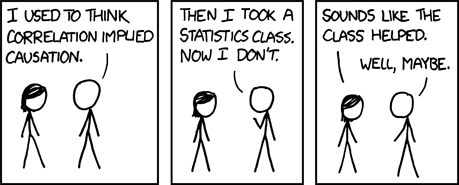
\includegraphics{figures/correlation}

\}

\textbackslash caption\{\emph{Correlation does not imply causation}, ontleend met toestemming aan \url{http://xkcd.com/552}.\}\label{fig:xkcd552}
\textbackslash end\{figure\}

\hypertarget{ch:betrouwbaarheid}{%
\chapter{Betrouwbaarheid}\label{ch:betrouwbaarheid}}

\hypertarget{inleiding-6}{%
\section{Inleiding}\label{inleiding-6}}

In Hoofdstuk \ref{ch:validiteit} hebben we het onder andere gehad over
construct-validiteit, de afstand tussen het bedoelde (theoretische)
concept of construct enerzijds, en de onafhankelijke of afhankelijke
variabele anderzijds. In dit hoofdstuk gaan we in op een ander zeer
belangrijk aspect van de afhankelijke variabele, nl. de
\emph{betrouwbaarheid}. Deze betrouwbaarheid kan worden geschat op basis van
de samenhang of correlatie tussen observaties van hetzelfde construct.
We zullen ook ingaan op de relaties tussen betrouwbaarheid en
constructvaliditeit.

Vaak worden validiteit en betrouwbaarheid in één adem genoemd, en in opeenvolgende hoofdstukken besproken. Daar is wat voor te zeggen, want beide begrippen gaan over hoe je je variabelen definieert en operationaliseert. Toch hebben we hier gekozen voor een andere volgorde. Betrouwbaarheid komt pas aan bod nadat we samenhang besproken hebben (Hoofdstuk \ref{ch:samenhang}), omdat betrouwbaarheid gebaseerd is op de samenhang of correlatie tussen observaties.

\hypertarget{wat-is-betrouwbaarheid}{%
\section{Wat is betrouwbaarheid?}\label{wat-is-betrouwbaarheid}}

Een betrouwbaar persoon is stabiel en voorspelbaar: wat hij of zij
vandaag doet is consistent met wat hij of zij vorige week deed, je kunt
op deze persoon vertrouwen --- in tegenstelling tot een onbetrouwbaar
persoon, die instabiel is en zich onvoorspelbaar gedraagt. Volgens \emph{Van
Dale} is \emph{betrouwbaarheid} ``\ldots de mate waarin iets of iem. te betrouwen
of geloofwaardig is''. Betrouwbare metingen kunnen de basis vormen voor
een ``justified true belief'' (zie
§\ref{sec:falsificatie}); onbetrouwbare metingen daarentegen zijn
per definitie niet waard om geloof aan te hechten.

Metingen vertonen altijd enige mate van fluctuatie of variatie of
inconsistentie. Die variabiliteit kan ten dele worden toegeschreven aan
de variatie in het gedrag dat gemeten wordt. Immers, zelfs als we
hetzelfde construct meten bij dezelfde persoon, dan nog zien we variatie
ten gevolge van de momentane mentale of fysieke toestand van de
proefpersoon, die nu eenmaal fluctueert. Bovendien is er variatie in het
gebruikte meet-instrument (thermometer, vragenlijst, sensor), en zijn er
wellicht inconsistenties in de wijze waarop wordt gemeten of beoordeeld.
Met de kwantificering van zulke consistenties en inconsistenties
betreden we het terrein van de betrouwbaarheidsanalyse.

Het begrip `betrouwbaarheid' heeft in wetenschappelijk onderzoek
eigenlijk twee betekenissen, die we afzonderlijk behandelen. Ten eerste
wordt met betrouwbaarheid de \emph{precisie} of \emph{nauwkeurigheid} van een
meting bedoeld. Dit aspect heeft betrekking op de vraag in hoeverre de
meting beïnvloed wordt door toevallige factoren (waardoor de meting niet
uitsluitend het onderzochte construct weergeeft). Als we \emph{niet}
nauwkeurig meten, dan weten we ook niet wat de verkregen meetwaarden
eigenlijk weergeven --- misschien het onderzochte construct, maar
misschien ook niet. Als we wel nauwkeurig meten, dan verwachten we, als
we dezelfde meting nogmaals zouden uitvoeren, dat we dan dezelfde
uitkomst zouden meten. Naarmate een meting minder precies is, zal er
meer variatie of inconsistentie zijn tussen de eerste meting en de
herhaalde meting, en zijn de metingen dus minder betrouwbaar.

\begin{center}\rule{0.5\linewidth}{0.5pt}\end{center}

\begin{quote}
\emph{Voorbeeld 12.1:} Als we de leesvaardigheid van
leerlingen in het eindexamen willen meten, dan leggen we hen een
tekstbegriptoets met een bijbehorend aantal vragen voor. De mate waarin
de verschillende vragen \emph{hetzelfde} construct meten, hier het construct `leesvaardigheid',
wordt de betrouwbaarheid, precisie of homogeniteit genoemd.
\end{quote}

\begin{center}\rule{0.5\linewidth}{0.5pt}\end{center}

In het vervolg zullen we, om verwarring te voorkomen, deze vorm van
betrouwbaarheid dan ook aanduiden met de term \emph{homogeniteit} (vs.
heterogeniteit). Bij een heterogene (niet-homogene) toets kan de
totaal-score moeilijk geïnterpreteerd worden. Bij een perfect homogene
test hebben mensen met dezelfde totaalscore ook dezelfde vragen correct
beantwoord. Maar als we menselijk (taal)gedrag meten, komen zulke
perfect homogene toetsen eigenlijk nooit voor: respondenten die wel
dezelfde totaalscore behalen, hebben toch niet allen dezelfde vragen
correct beantwoord (bv. in de leesvaardigheidstoets van het eindexamen,
voorbeeld 12.1). Dit houdt in dat de
vragen niet exact hetzelfde gemeten hebben. Dat is ook zo: de ene vraag
betrof een parafrase van een alinea, terwijl een andere vraag betrekking
had op een verwijswoord-antecedent-relatie. De vragen of items waren dus
niet perfect homogeen!

Ten tweede wordt met betrouwbaarheid de \emph{stabiliteit} van een meting
bedoeld. Om je gewicht te meten ga je op een weegschaal staan. Die
meting is stabiel: vijf minuten later zal dezelfde weegschaal met
dezelfde persoon onder dezelfde omstandigheden ook (bijna) dezelfde meetwaarde
opleveren. De stabiliteit wordt veelal uitgedrukt in een zogenaamde
correlatiecoëfficiënt (een maat voor samenhang, zie Hoofdstuk
\ref{ch:samenhang}). Deze correlatiecoëfficiënt kan alle waarden
aannemen tussen \(+1\) en \(-1\). Hoe meer de eerste en tweede meting gelijk
zijn, des te hoger de samenhang, en des te hoger de correlatie tussen
eerste en tweede meting. Omgekeerd, hoe lager de samenhang tussen eerste
en tweede meting, des te lager ook de correlatie.

Stabiele metingen komen echter zelden voor in onderzoek naar
(taal)gedrag. Als een toets tweemaal afgenomen wordt, dan is er vaak een
aanzienlijk verschil in scores op het eerste meetmoment en scores op het
tweede meetmoment.

\begin{center}\rule{0.5\linewidth}{0.5pt}\end{center}

\begin{quote}
\emph{Voorbeeld 12.2:}
Bij het eindexamen Nederlands moeten leerlingen een opstel schrijven,
dat wordt beoordeeld door twee beoordelaars. De beoordelaars zijn
stabiel, als zij na enige tijd dezelfde oordelen toekennen aan dezelfde
opstellen. Dus: als beoordelaar A eerst een 8 geeft aan een opstel, en
bij een tweede beoordeling enige tijd later ook een 8 geeft voor
hetzelfde opstel, dan is deze beoordelaar (zeer) stabiel. Als dezelfde
beoordelaar A bij de tweede beoordeling echter een 4 geeft aan ditzelfde
opstel, dan is de beoordelaar niet stabiel in zijn oordelen.
\end{quote}

\begin{quote}
Nu is het beoordelen van opstellen een lastige taak: de criteria zijn
niet scherp beschreven en er is relatief veel ruimte voor
interpretatie-verschillen. De stabiliteit van de oordelen is dan ook
laag; in het verleden is zelfs een stabiliteitscoëfficiënt van \(0.40\)
gerapporteerd.
\end{quote}

\begin{center}\rule{0.5\linewidth}{0.5pt}\end{center}

Om de stabiliteit van een toets te berekenen, moet dezelfde toets
tweemaal worden afgenomen; de mate van samenhang tussen de eerste en
tweede meting wordt de \emph{toets-hertoets-betrouwbaarheid} genoemd. Zo'n
herhaalde afname van een toets gebeurt in de praktijk zelden, vanwege de
relatief hoge kosten en relatief geringe opbrengst.

\begin{center}\rule{0.5\linewidth}{0.5pt}\end{center}

\begin{quote}
\emph{Voorbeeld 12.3:}
\citep{Lata09} ontwikkelden
een Spaanstalige vragenlijst van 39 vragen, bedoeld voor
afasie-patiënten om de kwaliteit van hun leven te bepalen. De kwaliteit
van leven wordt omschreven als ``the patient perception about, either the
effects of a given disease, or the application of a certain treatment on
different aspects of life, especially regarding its consequences on the
physical, emotional and social welfare'' \citep[ p.379]{Lata09}. De nieuwe
vragenlijst werd tweemaal afgenomen bij een steekproef van 23
Spaanstalige patiënten met afasie t.g.v. hersenbloeding. De
gerapporteerde test-hertest-stabiliteit voor deze vragenlijst was
\(0.95\).
\end{quote}

\begin{center}\rule{0.5\linewidth}{0.5pt}\end{center}

Zowel de homogeniteit als stabiliteit wordt uitgedrukt als een
coëfficient met een waarde tussen \(0\) en \(1\) (negatieve coëfficienten
komen in de praktijk niet voor). Hoe moeten we de gerapporteerde
coëfficienten nu interpreteren? In het algemeen geldt natuurlijk: hoe
hoger de coëfficient, hoe hoger (beter) de betrouwbaarheid. Maar hoe
groot moet de betrouwbaarheid minimaal zijn voordat we een toets
``betrouwbaar'' mogen noemen? Daar zijn geen eenduidige regels voor. Als
er afwegingen over personen gemaakt moeten worden, dan moet de toets een
betrouwbaarheid van minimaal \(0.90\) hebben, volgens het Nederlands
Instituut van Psychologen (NIP). Dat geldt bijvoorbeeld voor toetsen die
worden gebruikt om te bepalen of een kind wel of niet in aanmerking komt
voor een zgn. dyslexie-verklaring. Voor onderzoeksdoeleinden hoeft niet
zo'n strenge eis aan de betrouwbaarheid van een toets te worden gesteld.
Vaak wordt als ondergrens voor de betrouwbaarheidscoëfficient de waarde
\(0.70\) gehanteerd.

\hypertarget{testtheorie}{%
\section{Testtheorie}\label{testtheorie}}

De klassieke testtheorie heeft betrekking op de meting van variabele \(x\)
bij het \(i\)-de element van een steekproef van willekeurige leden uit een
populatie. De testtheorie poneert dat elke meting \(x_i\) samengesteld is
uit twee componenten, nl een ware score \(t_i\) (`true score') en een
foutscore of afwijking \(e_i\) (`error score'):
\begin{equation}
  x_i = t_i + e_i
  \label{eq:obs-true-error}
\end{equation}
Stel dat je ``in het echt'' \(t=72.0\) kg weegt, en stel
dat je gemeten gewicht \(x=71.6\) kg is, dan bedraagt de foutscore
\(e=-0.4\) kg.

Een eerste belangrijke aanname in de klassieke testtheorie is dat de
afwijkingen \(e_i\) elkaar neutraliseren of opheffen (d.w.z. gemiddeld nul
zijn, en dus niet systematisch afwijken van de ware score \(t\)), en dat
grotere afwijkingen naar boven of beneden minder vaker voorkomen dan
kleinere afwijkingen. Dat houdt in dat wordt aangenomen dat de
afwijkingen normaal verdeeld zijn (zie
§\ref{sec:normaalverdeling}), met \(\mu_e=0\) als gemiddelde:
\begin{equation}
  \label{eq:normal-error}
  e_i \sim \mathcal{N}(0,s^2_e)
\end{equation}

Een tweede belangrijke aanname in de klassieke testtheorie is dat er
geen verband is tussen de ware scores \(t_i\) en de foutscores \(e_i\).
Omdat de component \(e_i\) geheel door het toeval wordt bepaald, dus
zonder enig verband met \(x_i\), is de correlatie tussen de ware score en
de foutscore nul:
\begin{equation}
  \label{eq:r-true-error}
  r_{(t,e)} = 0
\end{equation}

De totale variantie van \(x\) is daarom\footnote{\(s^2_{(t+e)} = s^2_t + s^2_e + 2 r_{(t,e)} s_t s_e\), met hier \(r_{(t,e)}=0\) volgens formule \eqref{eq:r-true-error}.} gelijk aan som van de
variantie van de ware scores en de variantie van de foutscores:
\begin{equation}
  \label{eq:var-true-error}
  s^2_x = s^2_t + s^2_e
\end{equation}

Als de geobserveerde variantie \(s^2_x\) verhoudingsgewijs veel
fout-variantie bevat (d.i. variantie van afwijkingen), dan zijn de
geobserveerde scores goeddeels bepaald door toevallige afwijkingen. Dat
is natuurlijk geen wenselijke zaak. We zeggen dan dat de geobserveerde
scores niet betrouwbaar zijn; er zit veel ``ruis'' in de geobserveerde
scores. Als de fout-variantie daarentegen relatief gering is, dan geven
de geobserveerde scores goed weer wat de ware scores zijn, en dan zijn
de geobserveerde verschillen wel goed betrouwbaar, d.w.z. ze worden
weinig bepaald door toevallige afwijkingen.

We kunnen de betrouwbaarheid (symbool \(\rho\)) dan ook definiëren als de
verhouding tussen ware-score-variantie en totale variantie:
\begin{equation}
  \label{eq:rho-betrouwbaarheid}
  \rho_{xx} = \frac{s^2_t}{s^2_x}
\end{equation}

We kunnen deze formule \eqref{eq:rho-betrouwbaarheid} echter in de praktijk niet gebruiken
om de betrouwbaarheid vast te stellen, omdat we \(s^2_t\) niet kennen. We
moeten dus eerst schatten wat de ware-score-variantie is --- of wat de
fout-variantie is, die is immers het complement van de
ware-score-variantie (zie
formule \eqref{eq:var-true-error})\footnote{Een uitzondering hierop vormt de situatie indien \(s^2_x=0\), en dus \(s^2_t=0\), ergo betrouwbaarheid \(\rho=0\); de afhankelijke variabele \(x\) is dan niet goed geoperationaliseerd.}.

De tweede aanname (in formule \eqref{eq:r-true-error}) dat er geen verband is tussen de ware
score en de fout-score, is in de praktijk niet altijd gerechtvaardigd.
Dat wordt misschien inzichtelijk als we kijken naar de uitslagen van een
toets, op een schaal van 1.0 tot 10.0. De studenten met scores van 9 of
10 hebben ook een hoge ware score (zij beheersen de stof zeer goed) en
dus doorgaans een geringe fout-score. De studenten met scores van 1 of 2
hebben ook een lage ware score (zij beheersen de stof zeer slecht) en
dus ook doorgaans een geringe fout-score. Voor de studenten met scores
van 5 of 6 ligt de situatie anders: misschien beheersen ze de stof
redelijk goed maar hebben ze net een fout antwoord gegeven, of ze
beheersen de stof niet goed maar ze hebben toevallig een goed antwoord
gegeven. Voor deze studenten met een geobserveerde score in het midden
van de schaal zijn de fout-scores relatief groter dan voor de studenten
met een score bij de uiteinden van de schaal. In andere domeinen, bv bij
reactietijden, zien we andere verbanden, bv dat de foutscore min of meer
evenredig toeneemt met de score zelf; er is dan een positief verband
tussen de ware score en de foutscore (\(\rho_{(t,e)}>0\)). Desalniettemin
zijn de voordelen van de klassieke testtheorie zo groot dat we deze
theorie handhaven als uitgangspunt.

Uit de formules \eqref{eq:var-true-error} en \eqref{eq:rho-betrouwbaarheid}
hierboven volgt ook dat de standaard
meetfout (`standard error of measurement', ) gerelateerd is aan de
standaarddeviatie en aan de betrouwbaarheid:
\begin{equation}
   \label{eq:standaard-meetfout}
    s_e = s_x \sqrt{1-r_{xx}}
\end{equation}\\
Deze standaard meetfout is op te vatten
als de standaarddeviatie van de foutscores \(e_i\), nog steeds aannemende
dat de foutscores normaal verdeeld zijn (formule \eqref{eq:normal-error}).

\begin{center}\rule{0.5\linewidth}{0.5pt}\end{center}

\begin{quote}
\emph{Voorbeeld 12.4:}
Externe inspecteurs betwijfelen of docenten de eindwerkstukken van hun
studenten wel goed beoordelen. Als een student een 6 heeft gekregen, zou
dat werkstuk dan misschien eigenlijk als onvoldoende beoordeeld moeten
worden?
\end{quote}

\begin{quote}
Laten we aannemen dat de gegeven oordelen een standaarddeviatie
\(s_x=0.75\) vertonen, en laten we eveneens aannemen dat een analyse van
de betrouwbaarheid heeft laten zien dat \(r_{xx}=0.9\). De standaard
meetfout bedraagt dan \(s_e = 0.24\) punt (naar boven afgerond). De kans
dat de ware score \(t_i\) kleiner of gelijk is aan 5.4 (onvoldoende), bij
een geobserveerde score van \(x_i=6.0\) en \(s_e=0.24\), is slechts \(p=0.006\)
(voor uitleg, zie §\ref{sec:t-betrouwbaarheidsinterval-gemiddelde} hierna).
De voldoende beoordeling van het eindwerkstuk is met grote
waarschijnlijkheid juist.
\end{quote}

\begin{center}\rule{0.5\linewidth}{0.5pt}\end{center}

\hypertarget{interpretaties}{%
\section{Interpretaties}\label{interpretaties}}

Voordat we ingaan op verschillende berekeningswijzen van de
betrouwbaarheid is het zinvol om stil te staan bij verschillende
interpretaties van betrouwbaarheidsschattingen.

Ten eerste kan de betrouwbaarheid geïnterpreteerd worden als de
proportie ware-score-variantie (zie formule @ref (eq:rho-betrouwbaarheid)),
oftewel als de proportie van
variantie die ``systematisch'' is. Dit is vanzelfsprekend nog lang niet
hetzelfde als de proportie variantie ten gevolge van het
begrip-zoals-bedoeld, de ``valide'' variantie (zie
Hoofdstuk~\ref{ch:validiteit}). De variantie ten gevolge van het
begrip-zoals-bedoeld maakt deel uit van de proportie
ware-score-variantie. Echter, tal van andere factoren kunnen op
systematische wijze van invloed zijn op de scores van de respondenten,
zoals verschillen in toets-ervaring. Indien twee studenten \(i\) en \(j\)
een concept (zeg: taalvaardigheid) in dezelfde mate bezitten, dan nog
kan de ene student beter scoren omdat hij of zij vaker
taalvaardigheidstoetsen heeft afgelegd dan de andere student. Er is dan
geen verschil in het begrip zoals bedoeld (taalvaardigheid \(T_i = T_j\)),
maar wel in een andere factor (ervaring), en daardoor ontstaat een
verschil tussen de studenten in hun `ware' scores (\(t_i \neq t_j\)) die
we meten met een valide en betrouwbare taalvaardigheidsmeting. Bij die
meting treden afwijkingen en meetfouten op (\(e_i\) en \(e_j\)), waardoor de
geobserveerde verschillen tussen de studenten (\(x_i-x_j\)) groter of
kleiner kunnen zijn dan hun verschillen in `ware' score (\(t_i-t_j\)).
Vandaar dat een betrouwbaarheidsschatting altijd de bovengrens vormt van
de validiteit.

Een tweede interpretatie van de betrouwbaarheid (formule~\eqref{eq:rho-betrouwbaarheid})
is die van de theoretisch te verwachten correlatie (zie
§\ref{sec:Pearson}) tussen de metingen, bij vele herhalingen van
die metingen. Gemakshalve nemen we aan dat geheugen- en
vermoeidheidseffecten geen enkel effect hebben bij de tweede en latere
metingen. Als we dezelfde personen met hetzelfde instrument driemaal
zouden meten, zonder effecten van geheugen of vermoeidheid, dan zouden
de scores van de eerste en tweede meting, en van de eerste en derde
meting, en van de tweede en derde meting, steeds dezelfde correlatie
\(\rho\) vertonen. Die correlatie geeft dus aan in hoeverre de herhaalde
metingen consistent zijn, d.w.z. dezelfde onbekende ware score
representeren.

In deze interpretatie drukt de betrouwbaarheid dus de verwachte
samenhang uit tussen scores bij herhaalde afname van dezelfde toets. De
betrouwbaarheidscoëfficiënt \(\rho\) interpreteren we dan als de
correlatie tussen twee metingen met hetzelfde instrument.

Ten derde kan de betrouwbaarheid geïnterpreteerd worden als het verlies
van efficiëntie in het schatten van de gemiddelde score \(\overline{X}\)
\citep[ p.474]{Ferg89}. Stel dat we de gemiddelde score van een groep van
\(n=50\) proefpersonen willen vaststellen, en we gebruiken daarbij een
meetinstrument met betrouwbaarheid \(\rho_{xx}=0.8\). Er is dan
onzekerheid in de schatting, deels afkomstig van variatie in de ware
scores \(t_i\) van de proefpersonen, maar ook deels afkomstig van de
toevallige afwijkingen \(e_i\) bij de metingen. Als het meetinstrument
perfect betrouwbaar zou zijn (\(\rho=1\)) dan zouden we slechts
\(\rho_{xx}\times n = 0.8\times50=40\) proefpersonen nodig hebben gehad
voor dezelfde nauwkeurigheid van de schatting van \(\overline{X}\)
\citep[ p.474]{Ferg89}. We hebben dus als het ware 10 proefpersonen verspeeld
om te compenseren voor de onbetrouwbaarheid van het meetinstrument.

Hierboven hebben we gesproken over metingen met behulp van
meet-instrumenten, en hieronder zullen we spreken over beoordelingen
gedaan door beoordelaars. De benadering van de notie `betrouwbaarheid'
is in deze situaties steeds gelijk. Betrouwbaarheid speelt een rol in
alle situaties waarin elementen uit een steekproef worden gemeten of
beoordeeld door meerdere beoordelaars of instrumenten. Ook tentamina en
vragenlijsten kunnen zulke meetinstrumenten zijn: een tentamen of een
vragenlijst is goed te beschouwen als een samengesteld instrument
waarmee we een abstracte eigenschap of construct van de deelnemers
proberen te meten. Iedere vraag is dan te beschouwen als een
``meetinstrument'' of ``beoordelaar'' van de eigenschap of gesteldheid van
de respondent. Alle bovenvermelde inzichten en interpretaties aangaande
testtheorie, meetfout en betrouwbaarheid zijn daarbij evengoed van
toepassing.

\hypertarget{methoden-om-betrouwbaarheid-te-schatten}{%
\section{Methoden om betrouwbaarheid te schatten}\label{methoden-om-betrouwbaarheid-te-schatten}}

De betrouwbaarheid van een meting kan op verschillende manieren worden
bepaald. De belangrijkste zijn de volgende:

\begin{itemize}
\item
  De \emph{toets-hertoets-methode}\\
  We voeren alle metingen tweemaal uit, en berekenen daarna de
  correlatie tussen de eerste en de tweede meting. Naarmate de
  metingen minder meetfouten en afwijkingen bevatten, is de correlatie
  hoger en dus ook de betrouwbaarheid hoger. Deze methode is
  tijdrovend, maar kan ook worden toegepast op een kleine portie van
  de metingen. In spraak-onderzoek wordt deze methode wel gebruikt om
  de betrouwbaarheid van fonetische transcripties vast te stellen: een
  deel van de spraak-opnamen wordt door een tweede beoordelaar
  getranscribeerd, en vervolgens worden de beide transcripties
  vergeleken.
\item
  De \emph{parallelle-toetsvorm-methode}\\
  We hebben een grote verzameling meet-instrumenten die goed
  vergelijkbaar zijn en hetzelfde construct meten. We voeren alle
  metingen herhaaldelijk uit, de eerste keer door de metingen van
  enkele willekeurig getrokken meet-instrumenten te combineren (zeg A
  en B en C) en tweede keer met gebruik van andere willekeurige
  instrumenten (zeg D en E en F). Omdat de meetinstrumenten `parallel'
  zijn en hetzelfde construct worden geacht te meten, is de correlatie
  tussen de eerste en de tweede meting een indicatie voor de
  betrouwbaarheid van de meting.
\item
  De \emph{split-half-methode}\\
  Deze methode lijkt op de parallelle-toetsvorm-methode. De \(k\) vragen
  of instrumenten worden in twee helften verdeeld, waarna de score
  bepaald wordt binnen elke helft. Uit de correlatie \(r_{hh}\) tussen
  de scores op de twee halve toetsen kan de betrouwbaarheid van de
  gehele toets afgeleid worden, \(r_{xx} = \frac{2r_{hh}}{1+r_{hh}}\).
\end{itemize}

\hypertarget{betrouwbaarheid-tussen-beoordelaars}{%
\section{Betrouwbaarheid tussen beoordelaars}\label{betrouwbaarheid-tussen-beoordelaars}}

Laten we als voorbeeld eens kijken naar metingen van de
spreekvaardigheid van studenten in een vreemde taal. Dit construct
`spreekvaardigheid' wordt in dit voorbeeld gemeten door middel van twee
beoordelaars, die onafhankelijk van elkaar elk een cijfer tussen 1 en
100 geven aan de student (hoger is beter). Bij de beoordeling treden
echter ook meetfouten op, waardoor de oordelen niet alleen de
onderliggende ware score weergeven, maar ook een afwijking daarvan, met
alle hierboven genoemde aannames. Laten we eerst alleen kijken naar de
oordelen door de eerste en tweede beoordelaar (zie
Tabel~\ref{tab:betrouwbaarheid}). Het eindoordeel over een student is
vooralsnog het gemiddelde van de oordelen van de eerste en tweede
beoordelaar.

\begin{longtable}[]{@{}cccc@{}}
\caption{\label{tab:betrouwbaarheid} Oordelen over spreekvaardigheid van \(n = 10\) studenten (rijen) door
\(k = 3\) beoordelaars (kolommen).}\tabularnewline
\toprule
student & B1 & B2 & B3\tabularnewline
\midrule
\endfirsthead
\toprule
student & B1 & B2 & B3\tabularnewline
\midrule
\endhead
1 & 67 & 64 & 70\tabularnewline
2 & 72 & 75 & 74\tabularnewline
3 & 83 & 89 & 73\tabularnewline
4 & 68 & 72 & 61\tabularnewline
5 & 75 & 72 & 77\tabularnewline
6 & 73 & 73 & 78\tabularnewline
7 & 73 & 76 & 72\tabularnewline
8 & 65 & 73 & 72\tabularnewline
9 & 64 & 68 & 71\tabularnewline
10 & 70 & 82 & 69\tabularnewline
\(\overline{x_i}\) & 71.0 & 74.4 & 71.7\tabularnewline
\(s_i\) & 5.6 & 7.0 & 4.7\tabularnewline
\bottomrule
\end{longtable}

De oordelen van alleen de eerste en de tweede beoordelaar vertonen een
onderlinge correlatie van \(r_{1,2}=.75\). Dit houdt in (volgens
formule~\eqref{eq:rho-betrouwbaarheid}) dat 75\% van de totale variantie in
de oordelen van deze twee beoordelaars toe te schrijven is aan
verschillen tussen de beoordeelde studenten, en dus 25\% aan meetfouten
(we hebben immers aangenomen dat er geen systematische verschillen zijn
tussen beoordelaars). Het aandeel van de meetfouten lijkt nogal hoog. We
mogen echter wel hoop putten uit één van onze eerdere aannames, nl dat
de meetfouten van de beoordelaars niet gecorreleerd zijn. De
\emph{combinatie} van de twee beoordelaars --- de gemiddelde score per
student over de twee beoordelaars --- geeft dus beter betrouwbare
metingen dan elk van de beoordelaars afzonderlijk kunnen doen. Immers,
de meetfouten van de twee beoordelaars hebben de neiging om elkaar op te
heffen (zie formule~\eqref{eq:normal-error}).
Lees de laatste twee zinnen nog eens aandachtig door.

De betrouwbaarheid wordt vaak uitgedrukt als \emph{Cronbach's Alpha}
\citep{Cort93}. Dat getal is een maat voor de consistentie of homogeniteit
van de metingen, en het geeft dus ook de mate aan waarin de twee
beoordelaars hetzelfde construct hebben beoordeeld. De eenvoudigste
definitie is gebaseerd op \(\overline{r}\), de gemiddelde correlatie
tussen metingen van \(k\) verschillende beoordelaars\footnote{In ons voorbeeld zijn er slechts \(k=2\) beoordelaars, dus is er slechts één correlatie, en \(\overline{r} = r_{1,2} = 0.75\).}.
\begin{equation}
  \label{eq:cronbach-corr}
  \alpha = \frac{k \overline{r}} {1+(k-1)\overline{r}}
\end{equation}
Invullen van \(k=2\) beoordelaars en \(\overline{r}=0.75\) geeft \(\alpha=0.86\) (SPSS en R
gebruiken hiervoor een wat complexere formule, en rapporteren
\(\alpha=0.84\)). Deze maat voor betrouwbaarheid wordt niet alleen
aangeduid als Cronbach's Alpha, maar ook als de Spearman-Brown-formule
of als Kuder-Richardson-formule 20 (KR20)\footnote{De zgn. `intra-class correlation coefficient' (ICC) voor \(k\) vaste beoordelaars of items is eveneens identiek aan de Cronbach's Alpha.}.

De gevonden waarde van Cronbach's Alpha is wat lastig te evalueren,
omdat die mede afhankelijk is van het aantal instrumenten of
beoordelaars of vragen in de toets \citep{Cort93, Glin01}. Voor
wetenschappelijk onderzoek wordt vaak een ondergrens van 0.75 of 0.80
gehanteerd. Indien de uitslag van de toets of meting van groot belang is
voor de betrokkene, zoals bij medische of psychische diagnostiek van
patiënten, of bij werving en selectie van personeel, dan wordt een nog
hogere betrouwbaarheid van \(\alpha=.9\) aanbevolen \citep{Glin01}.

Als we de betrouwbaarheid willen verhogen naar \(\alpha=0.9\) of hoger,
dan kunnen we dat op twee manieren bereiken. De eerste manier is door
het aantal beoordelaars uit te breiden. Als we meer beoordelaars
combineren in de totale score, dan heffen de meetfouten van die
beoordelaars elkaar ook beter op, en dan wordt de totale score dus
betrouwbaarder. Met behulp van
formule~\eqref{eq:cronbach-corr} kunnen we onderzoeken hoeveel beoordelaars
nodig zouden zijn, om de betrouwbaarheid te verbeteren naar
\(\alpha=0.90\) of beter. We vullen \(\alpha=0.90\) in en wederom
\(\overline{r}=0.75\), en vinden dan een uitkomst van minimaal \(k=3\)
beoordelaars. De \emph{toename} in de betrouwbaarheid vlakt af naarmate er al
meer beoordelaars meedoen: als \(k=2\) dan \(\alpha=.84\), als \(k=3\) dan
\(\alpha=.84+.06=.90\), als \(k=6\) dan \(\alpha=.90+.05=.95\), als \(k=9\) dan
\(\alpha=.95+.01=.96\), enz. Immers, als er al 6 beoordelaars zijn, die
elkaars meetfouten al goed opheffen, dan voegen 3 extra beoordelaars
weinig meer toe aan de betrouwbaarheid.

De tweede manier om de betrouwbaarheid te verhogen is om de meetfout te
verkleinen. Dat kunnen we proberen, bijvoorbeeld, door de beoordelaars
zo goed mogelijk te instrueren over hoe ze de spreekvaardigheid van de
studenten dienen te beoordelen. Een beoordelingsprotocol en/of
instructie kan de afwijkingen tussen en binnen beoordelaars doen
verkleinen. Kleinere afwijkingen betekenen kleinere meetfouten, en dat
betekent weer hogere correlaties tussen de beoordelaars. Bij een
\(\overline{r}=0.8\) bereiken we al bijna de gewenste betrouwbaarheid, met
slechts \(k=2\) beoordelaars.

Een derde manier om de betrouwbaarheid te verhogen vereist een nadere
analyse van de afzonderlijke beoordelaars. Om dit uit te leggen,
betrekken we nu ook de derde beoordelaar in onze beschouwingen (zie
Tabel~\ref{tab:betrouwbaarheid}). De oordelen van deze derde
beoordelaar vertonen echter lage correlaties met die van de eerste en
tweede beoordelaar: \(r_{1,3}=0.41\) en \(r_{2,3}=0.09\). Dat leidt ertoe
dat de gemiddelde correlatie tussen beoordelaars nu lager is,
\(\overline{r}=0.42\). Door deze derde beoordelaar op te nemen, is de
betrouwbaarheid niet gestegen maar daarentegen juist gedaald naar
\(\alpha = \frac{3\times0.42}{1+2\times0.42} = 0.68\). We doen er dus
misschien beter aan om de metingen van de derde beoordelaar te negeren.
Ook als we de betrouwbaarheid van een tentamen of toets of vragenlijst
onderzoeken, kan blijken dat de betrouwbaarheid van de gehele toets
\emph{toeneemt} als we sommige ``slechte'' vragen verwijderen. Blijkbaar hebben
die ``slechte'' vragen een construct gemeten dat verschilt van wat de
resterende vragen gemeten hebben.

\hypertarget{betrouwbaarheid-en-constructvaliditeit}{%
\section{Betrouwbaarheid en constructvaliditeit}\label{betrouwbaarheid-en-constructvaliditeit}}

Als een meting betrouwbaar is, dan is er ``iets'' betrouwbaar gemeten.
Maar let op: dat toont nog niet aan \emph{wat} er gemeten is! Er is wel een
relatie tussen de betrouwbaarheid (hoe is gemeten) en de
construct-validiteit (wat is gemeten, zie
Hoofdstuk~\ref{ch:validiteit}), maar die twee begrippen zijn niet identiek.
Een voldoende betrouwbaarheid is een noodzakelijke, maar geen voldoende
voorwaarde voor validiteit. Anders gezegd: een toets die niet
betrouwbaar is kan ook niet valide zijn (want deze toets meet ook ruis),
maar een toets die wel betrouwbaar is hoeft nog niet valide te zijn.
Misschien meet de gebruikte toets wel heel betrouwbaar een ander
construct dan wat de bedoeling was.

Een instrument is construct-valide als het gemeten concept overeenkomt
met het bedoelde concept of construct. In
voorbeeld 12.3: de vragenlijst is valide als score uit de
vragenlijst overeenkomt met de kwaliteit van leven (wat dat dan ook moge
zijn) van de afasie-patiënten. Pas nadat aangetoond is dat een
instrument betrouwbaar is, heeft het zin om over de constructvaliditeit
van een meting te spreken. De betrouwbaarheid is een noodzakelijke maar
niet voldoende voorwaarde voor constructvaliditeit. Een onbetrouwbaar
instrument kan dus niet valide zijn, maar een betrouwbaar instrument
hoeft niet noodzakelijk valide te zijn.

Om de schrijfvaardigheid te meten, laten we de leerlingen een opstel
schrijven. We tellen het aantal letters \emph{e} in elk opstel. Dat is een
zeer betrouwbare meting: verschillende beoordelaars komen tot hetzelfde
aantal \emph{e}'s (beoordelaars zijn homogeen) en dezelfde beoordelaar levert
bij hetzelfde opstel ook steeds dezelfde uitkomst (beoordelaars zijn
stabiel). Het grote bezwaar hier is dat het aantal \emph{e}'s in een opstel
niet of niet noodzakelijk overeenkomt met het concept
schrijfvaardigheid. Een leerling die meer \emph{e}'s in zijn opstel verwerkt
is niet noodzakelijk een betere schrijver.

Onderzoekers weten weliswaar dat betrouwbaarheid een noodzakelijke maar
niet voldoende voorwaarde is voor de validiteit. Maar toch springen ze
niet altijd even zorgvuldig om met die begrippen. In vele onderzoeken
wordt er stilzwijgend van uit gegaan dat als de betrouwbaarheid
voldoende is, de validiteit dan ook gewaarborgd is. Ook in voorbeeld 12.3
wordt het onderscheid niet duidelijk gemaakt,
en bespreken de onderzoekers de construct-validiteit van hun nieuwe
vragenlijst niet expliciet.

\hypertarget{spss-9}{%
\section{SPSS}\label{spss-9}}

Voor een betrouwbaarheidsanalyse van de \(k=3\) oordelen over
spreekvaardigheid in
Tabel~\ref{tab:betrouwbaarheid}:\\

\begin{verbatim}
Analyze > Scale > Reliability Analysis...
\end{verbatim}

Selecteer de variabelen die geacht worden hetzelfde construct te meten;
hier zijn dat de drie beoordelaars. We beschouwen deze \(k=3\)
beoordelaars als ``items'' die de eigenschap ``spreekvaardigheid'' meten van
10 studenten. Sleep deze variabelen naar het Variable(s) paneel.\\
Vul als Scale label in een aanduiding van het construct, bijv.
\texttt{Spreekvaardigheid}.\\
Kies als Method: \texttt{Alpha} voor Cronbach's Alpha (zie formule
\eqref{eq:cronbach-corr})\\
Kies \texttt{Statistics\ldots{}}, vink aan: Descriptives for
\texttt{Item,\ Scale,\ Scale\ if\ item\ deleted}, Inter-Item \texttt{Correlations},
Summaries \texttt{Means,\ Variances}, en bevestig met \texttt{Continue} en daarna
nogmaals met \texttt{OK}.

De uitvoer bevat Cronbach's Alpha, de gevraagde
inter-item-correlaties (vooral hoog tussen beoordelaars 1 en 2), en (in
tabel Item-Total Statistics) de betrouwbaarheid indien we een bepaalde
beoordelaar zouden verwijderen. Deze laatste uitvoer leert ons dat
beoordelaars 1 en 2 van groter belang zijn dan beoordelaar 3. Als we
beoordelaar 1 of 2 zouden verwijderen dan stort de betrouwbaarheid in,
maar als we beoordelaar 3 zouden verwijderen dan neemt de
betrouwbaarheid zelfs toe (van 0.68 naar 0.84). Vermoedelijk heeft deze
beoordelaar een ander construct beoordeeld dan de anderen.

\hypertarget{r-10}{%
\section{R}\label{r-10}}

Voor een betrouwbaarheidsanalyse van de \(k=3\) oordelen over
spreekvaardigheid in Tabel \ref{tab:betrouwbaarheid}:\\

\begin{Shaded}
\begin{Highlighting}[]
\NormalTok{beoordelaars \textless{}{-}}\StringTok{ }\KeywordTok{read.table}\NormalTok{(}\DataTypeTok{file=}\StringTok{"data/beoordelaars.txt"}\NormalTok{, }\DataTypeTok{header=}\OtherTok{TRUE}\NormalTok{)}
\ControlFlowTok{if}\NormalTok{ (}\KeywordTok{require}\NormalTok{(psych)) \{ }\CommentTok{\# voor psych::alpha}
  \KeywordTok{alpha}\NormalTok{( beoordelaars[,}\DecValTok{2}\OperatorTok{:}\DecValTok{4}\NormalTok{] ) }\CommentTok{\# kolommen 2 t/m 4}
\NormalTok{\}}
\end{Highlighting}
\end{Shaded}

\begin{verbatim}
## Number of categories should be increased  in order to count frequencies.
\end{verbatim}

\begin{verbatim}
## 
## Reliability analysis   
## Call: alpha(x = beoordelaars[, 2:4])
## 
##   raw_alpha std.alpha G6(smc) average_r S/N  ase mean  sd median_r
##       0.68      0.68    0.74      0.41 2.1 0.17   72 4.6     0.41
## 
##  lower alpha upper     95% confidence boundaries
## 0.35 0.68 1.01 
## 
##  Reliability if an item is dropped:
##    raw_alpha std.alpha G6(smc) average_r  S/N alpha se var.r med.r
## B1      0.15      0.16   0.088     0.088 0.19    0.497    NA 0.088
## B2      0.58      0.58   0.410     0.410 1.39    0.264    NA 0.410
## B3      0.84      0.85   0.745     0.745 5.84    0.095    NA 0.745
## 
##  Item statistics 
##     n raw.r std.r r.cor r.drop mean  sd
## B1 10  0.93  0.92  0.91   0.81   71 5.6
## B2 10  0.84  0.78  0.72   0.53   74 7.0
## B3 10  0.56  0.64  0.38   0.25   72 4.7
\end{verbatim}

Deze uitvoer bevat Cronbach's Alpha (\texttt{raw\_alpha\ 0.68}), en de
betrouwbaarheid indien we een bepaalde beoordelaar zouden verwijderen.
Als we beoordelaar 3 zouden verwijderen dan neemt de betrouwbaarheid
zelfs toe (van 0.68 naar 0.84). Over alle drie de beoordelaars is
\texttt{average\_r=0.41}.

Correlaties tussen de \(k\) beoordelaars of items worden niet expliciet
meegeleverd (al zijn ze wel af te leiden uit bovenstaande uitvoer), dus
vragen we die nog op:

\begin{Shaded}
\begin{Highlighting}[]
\KeywordTok{cor}\NormalTok{( beoordelaars[ ,}\KeywordTok{c}\NormalTok{(}\StringTok{"B1"}\NormalTok{,}\StringTok{"B2"}\NormalTok{,}\StringTok{"B3"}\NormalTok{) ] ) }\CommentTok{\# expliciete kolomnamen}
\end{Highlighting}
\end{Shaded}

\begin{verbatim}
##           B1         B2         B3
## B1 1.0000000 0.74494845 0.40979738
## B2 0.7449484 1.00000000 0.08845909
## B3 0.4097974 0.08845909 1.00000000
\end{verbatim}

\begin{center}\rule{0.5\linewidth}{0.5pt}\end{center}

\hypertarget{part-deel-iii-toetsende-statistiek}{%
\part*{Deel III: Toetsende statistiek}\label{part-deel-iii-toetsende-statistiek}}
\addcontentsline{toc}{part}{Deel III: Toetsende statistiek}

\hypertarget{ch:toetsing}{%
\chapter{Toetsing}\label{ch:toetsing}}

\hypertarget{sec:toetsing-inleiding}{%
\section{Inleiding}\label{sec:toetsing-inleiding}}

Vanaf dit hoofdstuk houden we ons bezig met het toetsen van
onderzoekshypothesen, en in het bijzonder met toetsen van \emph{nul}-hypotheses (null hypothesis significance testing, NHST), zoals uitgelegd in Hoofdstuk \ref{ch:onderzoek}.

Voor dergelijke toetsingen is in de loop der jaren
een groot aantal technieken ontwikkeld. De toetsen die we behandelen
zijn de meest gebruikte en kunnen we indelen in parametrische en
non-parametrische toetsen. Parametrische toetsen veronderstellen dat de
afhankelijke variabele (tenminste) gemeten is op intervalniveau (zie
hoofdstuk~\ref{ch:Meetniveau}), en dat de gemeten uitkomsten of scores
normaal verdeeld zijn (zie
§\ref{sec:normaalverdeling} en
§\ref{sec:watalsnietnormaal}). Bij non-parametrische toetsen
worden, afhankelijk van de techniek, minder aannamen gemaakt over het
meetniveau, danwel over de verdeling van de geobserveerde scores; het
zijn zogenaamde verdelingsvrije toetsen. Het gevolg is dat de toetsing
iets minder `gevoelig' is, onder verder gelijke omstandigheden, d.w.z.
dat de nulhypothese onder verder gelijke omstandigheden minder vaak
verworpen kan worden. Deze toetsen hebben derhalve minder power (zie
Hoofdstuk \ref{ch:power}). Onderzoekers geven daarom meestal de voorkeur
aan parametrische toetsen.

Het algemene principe van toetsing hebben we al kort besproken in
§\ref{sec:falsificatie} en
§\ref{sec:empirischecyclus}.
We leggen het hier nogmaals uit aan
de hand van een voorbeeld. We onderzoeken de bewering H1: `studenten
Taalwetenschap beheersen de traditionele zinsgrammatica \emph{beter} dan de
gemiddelde talen-student'. Als meet-instrument gebruiken we de zgn.
``grammaticatoets''\footnote{Wij danken Els Rose voor het beschikbaar stellen van deze gegevens.} die verplicht is voor de meeste studenten in het
talen-domein van de Universiteit Utrecht. Op grond van eerdere
studiejaren verwachten we een gemiddelde score van 73 op deze toets; dit
is het gemiddeld aantal goede antwoorden uit 100 vragen. We
operationaliseren dus eerst H1: \(\mu > 73\), en daaruit leiden we de
bijbehorende nulhypothese af die daadwerkelijk getoetst wordt:
\(\mu = 73\).
(In~§\ref{sec:ttoets-eenzijdigtweezijdig} hieronder gaan we nader in
op het al dan niet noemen van de \emph{richting} van het verschil in H1).

Voor de
eerstejaars studenten Taalwetenschap (\(n=34\)) van een bepaald studiejaar
vinden we een gemiddelde score van 84.4. Dat is inderdaad ver boven de
referentie-waarde van 73, maar dat zou ook toeval kunnen zijn. Misschien
is H0 waar, en zitten er geheel toevallig veel grammaticale bollebozen
in onze steekproef (uit de populatie van mogelijke eerstejaars studenten
Taalwetenschap). We kunnen de kans \(P\) op die situatie uitrekenen,
d.w.z. de kans \(P\) om een gemiddelde score van \(\overline{x}=84.4\) te
vinden gegeven een willekeurige steekproef van \(n=34\) personen en
gegeven dat H0 in werkelijkheid waar is (d.w.z. \(\mu=73\)): dan blijkt
\(P=.000000001913\). Deze kans \(P\) representeert de kans om bij toeval
deze gegevens te vinden terwijl H0 waar is:
\(P(\overline{x}=84.4|\textrm{H0},n=34)\). In dit geval is die kans \(P\)
zeer klein.

Voor de argumentatie is het essentieel dat de gegevens valide zijn en
betrouwbaar zijn --- juist daarom zijn we uitgebreid ingegaan op
validiteit
(Hoofdstuk \ref{ch:validiteit}) en betrouwbaarheid
(Hoofdstuk~\ref{ch:betrouwbaarheid}). Als we alles goed gedaan hebben, dan
mogen we immers vertrouwen hebben in onze verkregen gegevens. De lage
waarschijnlijkheid van de gegevens volgens H0 kunnen we dan
redelijkerwijs \emph{niet} toeschrijven aan fouten in de operationalisatie,
of aan meetfouten, of aan andere afwijkingen in de gegevens. De logische
conclusie is dan, dat de onwaarschijnlijke uitkomst erop wijst dat de
premisse (H0) waarschijnlijk \emph{niet} waar is: we verwerpen H0; H0 is dus
gefalsifieerd. Onze kennis is daarmee toegenomen, omdat we nu op
gerechtvaardigde gronden mogen aannemen dat H0 onwaar is (en dus dat H1
waar is).

Indien we H0 verwerpen, op basis van bovenstaande redenering, die weer
gebaseerd is op waarschijnlijkheid, dan moeten we wel rekening houden
met de kleine kans \(P\) dat het verwerpen van H0 een onterechte
beslissing is (Type-I-fout; zie
§\ref{sec:empirischecyclus}). Er is immers de kans \(P\) dat we deze
data vinden terwijl H0 toch waar is (in dit voorbeeld: terwijl de
taalwetenschappers eigenlijk gemiddeld niet anders scoren dan \(\mu=73\)).

\begin{figure}
\centering
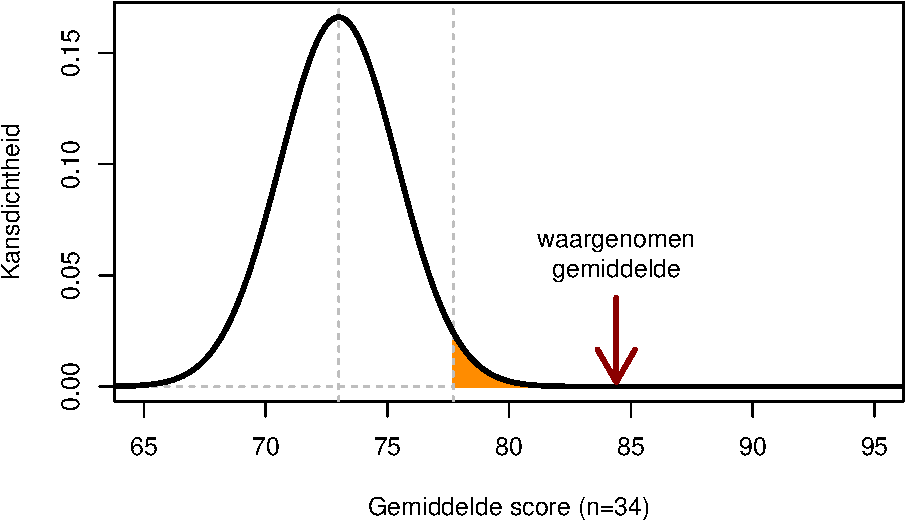
\includegraphics{KMS-NL_files/figure-latex/gramm2013onesample-1.pdf}
\caption{\label{fig:gramm2013onesample}Kansverdeling van de gemiddelde score uit een steekproef (n=34) bij populatiegemiddelde 73 en populatie-s.d. 14. Het gekleurde gebied bestrijkt 5\% van de totale oppervlakte onder de curve; uitkomsten langs de X-as van dit gebied hebben dus een kans van ten hoogste 5\% om op te treden als H0 waar is.}
\end{figure}

Figuur~\ref{fig:gramm2013onesample} toont de kansverdeling van het
gemiddelde van de steekproef (\(n=34\)) als H0 waar is. We zien dat de
waarde 73 de hoogste kans heeft, maar ook 72 of 74 zijn waarschijnlijke
gemiddelde scores volgens H0. Een gemiddelde van 84.4 is echter zeer
onwaarschijnlijk, de kans \(P\) op deze gemiddelde score (hoogte van de
curve) is bijna nul volgens H0.

De grenswaarde voor \(P\) waarbij we H0 verwerpen, wordt het
significantieniveau genoemd, vaak aangeduid met symbool \(\alpha\) (zie
§\ref{sec:empirischecyclus}). Onderzoekers gebruiken vaak
\(\alpha=.05\), maar soms worden andere grenswaarden gebruikt. In
Figuur~\ref{fig:gramm2013onesample} zie je dat de kans op een gemiddelde
score van 77.7 of meer een kans heeft van \(P=.05\) of kleiner, volgens
H0. Dit is te zien aan de oppervlakte onder de curve. Het gekleurde deel
heeft precies een oppervlakte van 0.05 van de totale oppervlakte onder
de curve.

De beslissing om H0 wel of niet te verwerpen is gebaseerd op de
waarschijnlijkheid \(P\) van de uitkomsten, gegeven H0. De beslissing zou
dus ook onjuist kunnen zijn. De bevinding dat \(P < \alpha\) vormt dus
geen \emph{onomstotelijk} bewijs dat H0 onwaar is (en verworpen \emph{moet}
worden); het is ook mogelijk dat H0 toch waar is maar dat het gevonden
effect een toevalstreffer was (Type-I-fout). Omgekeerd vormt de
bevinding dat \(P > \alpha\) geen sluitend bewijs dat H0 waar is. Er
kunnen allerlei andere, plausibele redenen zijn waarom een wel bestaand
effect (H0 is onwaar) toch niet goed geobserveerd wordt. Als ik geen
vogels hoor zingen, dan betekent dat niet noodzakelijkerwijs dat er echt
geen vogels zingen. Meer algemeen: ``absence of evidence is not evidence
of absence'' \citetext{\citealp[p.121]{Sagan96}; \citealp{Alde04}}. Het is daarom goed om ook altijd de grootte van het
gevonden effect of verschil te rapporteren (dit wordt nader uitgelegd in
§\ref{sec:ttoets-effectgrootte} hieronder).

\begin{center}\rule{0.5\linewidth}{0.5pt}\end{center}

\begin{quote}
\emph{Voorbeeld 13.1:}
Stel H0: `vogels zingen niet'. Schrijf
tenminste vier redenen op waarom ik geen vogels hoor zingen, zelfs als
er wel vogels zingen (H0 is onwaar). Als ik H0 niet verwerp, wat voor
type fout maak ik dan?
\end{quote}

\begin{center}\rule{0.5\linewidth}{0.5pt}\end{center}

\hypertarget{sec:ttoets-onesample}{%
\section{\texorpdfstring{\(t\)-toets voor enkele steekproef}{t-toets voor enkele steekproef}}\label{sec:ttoets-onesample}}

De Student \(t\)-toets wordt toegepast om een verschil te kunnen onderzoeken tussen
de gemiddelde score van een steekproef, en een a priori veronderstelde
waarde van dat gemiddelde. We gebruiken deze toets als de
standaarddeviatie \(\sigma\) in de populatie niet bekend is, en dus
geschat moet worden uit de steekproef. De gedachtegang is als volgt.

Op grond van het gemiddelde en de standaarddeviatie in de steekproef, en
van het (volgens H0) veronderstelde gemiddelde, bepalen we de toetsingsgrootheid \(t\).
Als H0 waar is, dan is de waarde \(t=0\) het meest waarschijnlijk.
Naarmate het verschil tussen het geobserveerde steekproefgemiddelde en
het veronderstelde steekproefgemiddelde groter wordt, neemt \(t\) ook toe.
Als de toetsingsgrootheid \(t\) groter is dan een bepaalde grenswaarde
\(t*\), dus als \(t>t*\), dan is de kans op deze toetsingsgrootheid, als H0
waar is, erg klein: \(P(t|\textrm{H0}) < \alpha\). De kans om dit
resultaat te vinden als H0 waar is, is dan zo gering dat we besluiten H0
te verwerpen (zie
§\ref{sec:empirischecyclus}). We spreken dan van een \emph{significant}
verschil: de afwijking tussen het geobserveerde en het verwachte
gemiddelde is vermoedelijk niet toevallig.

In het eerdere voorbeeld van de grammaticatoets bij studenten
Taalwetenschap (§\ref{sec:toetsing-inleiding}) hebben we al kennis gemaakt met
deze vorm van de \(t\)-toets.
Als \(\overline{x}=84.4, s=8.4, n=34\), dan is
toetsingsgrootheid \(t=7.9\) volgens formule \eqref{eq:t-onesample} hieronder.

De kansverdeling van toetsingsgrootheid \(t\) onder H0 is bekend; je vindt
de grenswaarde \(t^*\) in
Bijlage~\ref{app:kritieketwaarden}. Anders gezegd, als de gevonden
toetsingsgrootheid \(t\) groter is dan de grenswaarde \(t^*\) die in de
tabel staat vermeld, dan is \(P(t|\textrm{H0})<\alpha\). Om de tabel in
Bijlage~\ref{app:kritieketwaarden} te kunnen gebruiken moeten we nog een
nieuw begrip introduceren, namelijk het aantal vrijheidsgraden. Dat
begrip wordt uitgelegd in
§\ref{sec:ttoets-vrijheidsgraden} hieronder.

Met het aantal vrijheidsgraden kun je in
Bijlage~\ref{app:kritieketwaarden} opzoeken welke grenswaarde \(t^*\) nodig
is om een bepaalde overschrijdingskans \(p\) te verkrijgen. Laten we
opzoeken wat de overschrijdingskans is voor de gevonden
toetsingsgrootheid \(t=7.9\). Eerst zoeken we in de linker kolom het
aantal vrijheidsgraden (`d.f.') op. Als het aantal vrijheidsgraden niet
in de tabel voorkomt, dan dienen we voorzichtigheidshalve naar beneden
af te ronden, hier naar 30 d.f. Dit aantal bepaalt de regel die voor ons
van toepassing is. In de derde kolom staat \(t^*=1.697\). Onze gevonden
toetsingsgrootheid \(t=7.9\) is groter dan deze \(t^*=1.697\), dus de
overschrijdingskans is kleiner dan de \(p=.05\) die hoort bij de derde
kolom. Als we verder naar rechts gaan op dezelfde regel, zien we dat de
vermelde \(t^*\) nog toeneemt. Onze gevonden toetsingsgrootheid \(t\) is
zelfs nog groter dan \(t^*=3.385\) in de laatste kolom. De
overschrijdingskans is dus zelfs nog kleiner dan \(p=.001\) uit de titel
van die laatste kolom. (Doorgaans berekent het statistische
analyse-programma ook de overschrijdingskans.) We rapporteren het
resultaat als volgt:

\begin{quote}
De gemiddelde score van de studenten Taalwetenschap (lichting 2013) is
84.4 (\(s=8.4\)); dit is significant beter dan het veronderstelde
populatie-gemiddelde van 73 (\(t(33)=7.9, p<.001\)).
\end{quote}

\hypertarget{sec:ttoets-vrijheidsgraden}{%
\subsection{vrijheidsgraden}\label{sec:ttoets-vrijheidsgraden}}

Om het concept van vrijheidsgraden uit te leggen, beginnen we met een
analogie. Stel dat er drie mogelijke routes zijn om van A naar B te
reizen: een kustpad, een bergpad, of een autoweg. Een wandelaar die van
A naar B wil reizen, heeft weliswaar drie opties, maar er zijn slechts
twee vrijheidsgraden voor de wandelaar: hij of zij hoeft slechts 2
keuzes te maken om te kiezen uit de drie opties. Eerst valt de autoweg
af (eerste kies-moment), en dan het bergpad (tweede kies-moment), en de
gekozen route langs het kustpad blijft als enige over. Er zijn dus twee
keuzes `vrij', om uiteindelijk één van de drie mogelijke routes te
kiezen. Als we de twee keuzes weten, dan kunnen we daaruit afleiden
welke route gekozen moet zijn.

Nu kijken we naar een student die gemiddeld een \(\overline{x}=7.0\) heeft
behaald over de \(N=4\) cursussen van het eerste basispakket van zijn of
haar opleiding. Het gemiddelde van \(7.0\) kan op vele manieren tot stand
zijn gekomen, bv. \((8,7,7,6)\) of \((5,6,8,9)\). Maar als we van drie
cursussen het resultaat weten, èn we weten dat het gemiddelde een 7.0
bedraagt, dan weten we ook wat de waarde van de vierde observatie moet
zijn. Die laatste observatie is dus niet meer `vrij' maar wordt nu
vastgelegd door de eerste drie observaties, in combinatie met het
gemiddelde over de \(N=4\) observaties. We zeggen dan dat je \(N-1\)
\emph{vrijheidsgraden} hebt om dit kenmerk van de steekproef te bepalen,
zoals hier het steekproefgemiddelde, of zoals de toetsingsgrootheid \(t\).
De vrijheidsgraden worden in het Engels `degrees of freedom' genoemd,
vaak afgekort tot `d.f.' (symbool \(\nu\), griekse letter ``nu'') .

In de praktijk is het aantal vrijheidsgraden niet moeilijk te bepalen.
We geven namelijk bij elke toets aan hoe je de vrijheidsgraden bepaalt
--- en het aantal d.f. wordt doorgaans ook berekend door de statistische
analyse-programma's die we gebruiken.

Bij de \(t\)-toets voor een enkele steekproef is het aantal vrijheidsgraden het
aantal observaties \(N-1\). In het hierboven besproken voorbeeld hebben we
dus \(N-1 = 34-1 = 33\) vrijheidsgraden.

\hypertarget{sec:formules13-1}{%
\subsection{formules}\label{sec:formules13-1}}

\begin{equation}
  t = \frac{ \overline{y}-\mu} { s } \times \sqrt{N}
  \label{eq:t-onesample}
\end{equation}

\hypertarget{sec:ttoets-aannames}{%
\subsection{aannames}\label{sec:ttoets-aannames}}

De \(t\)-toets voor een enkele steekproef vereist drie aannames (assumpties) waaraan
voldaan moet zijn, om de toets te mogen gebruiken.

\begin{itemize}
\item
  De gegevens moeten gemeten zijn op intervalniveau (zie
  hoofdstuk \ref{ch:Meetniveau}).
\item
  Alle observaties moeten onafhankelijk van elkaar zijn.
\item
  De scores moeten normaal verdeeld zijn (zie
  §\ref{sec:normaalverdeling}).
\end{itemize}

\hypertarget{spss-10}{%
\subsection{SPSS}\label{spss-10}}

De hierboven besproken gegevens zijn te vinden in het bestand \texttt{data/grammaticatoets2013.csv}.

Om onze eerdere hypothese te toetsen, moeten we in SPSS eerst de
observaties selecteren van de studenten Taalwetenschap.

\begin{verbatim}
Data > Select cases...
\end{verbatim}

Kies \texttt{If\ condition\ is\ satisfied} en druk op knop \texttt{If...} om de condities
voor selectie (inclusie) aan te geven.\\
Selecteer variabele \texttt{opleiding} (sleep naar rechter paneel), kies knop
\texttt{=}, en type daarna \emph{\texttt{TW}}, zodat de hele conditie luidt
\texttt{opleiding\ =\ TW}.

Daarna kunnen we onze eerdere hypothese toetsen als volgt:

\begin{verbatim}
Analyze > Compare Means > One-Sample T Test...
\end{verbatim}

Selecteer variabele (sleep naar Test variable(s) paneel).\\
Geef op tegen welke waarde van \(\mu\) getoetst moet worden: geef op als
Test Value \texttt{73}. Bevestig met \texttt{OK}.

De uitvoer bevat zowel beschrijvende statistiek als de resultaten van
een \emph{tweezijdige} \(t\)-toets.

Neem bij het overnemen van die uitvoer goede notitie van de waarschuwing in
§\ref{sec:pgroterdannul} hieronder: SPSS rapporteert alsof \texttt{p=.000} maar dat is onjuist.

\hypertarget{jasp}{%
\subsection{JASP}\label{jasp}}

Hier komen JASP instructies.

\hypertarget{r-11}{%
\subsection{R}\label{r-11}}

Onze hierboven besproken hypothese kan worden getoetst met de volgende opdrachten:

\begin{Shaded}
\begin{Highlighting}[]
\NormalTok{gramm2013 \textless{}{-}}\StringTok{ }\KeywordTok{read.csv}\NormalTok{( }\DataTypeTok{file=}\StringTok{"data/grammaticatoets2013.csv"}\NormalTok{,}\DataTypeTok{header=}\NormalTok{F)}
\KeywordTok{dimnames}\NormalTok{(gramm2013)[[}\DecValTok{2}\NormalTok{]] \textless{}{-}}\StringTok{ }\KeywordTok{c}\NormalTok{(}\StringTok{"score"}\NormalTok{,}\StringTok{"opleiding"}\NormalTok{)}
\KeywordTok{with}\NormalTok{( gramm2013,}
      \KeywordTok{t.test}\NormalTok{( score[opleiding}\OperatorTok{==}\StringTok{"TW"}\NormalTok{], }\DataTypeTok{mu=}\DecValTok{73}\NormalTok{, }\DataTypeTok{alt=}\StringTok{"greater"}\NormalTok{ ) )}
\end{Highlighting}
\end{Shaded}

\begin{verbatim}
## 
##  One Sample t-test
## 
## data:  score[opleiding == "TW"]
## t = 7.9288, df = 33, p-value = 1.913e-09
## alternative hypothesis: true mean is greater than 73
## 95 percent confidence interval:
##  81.97599      Inf
## sample estimates:
## mean of x 
##  84.41176
\end{verbatim}

De notatie \texttt{1.913e-09} moet gelezen worden als het getal
\((1.913 \times 10^{-9})\).

\hypertarget{sec:pgroterdannul}{%
\section{\texorpdfstring{Overschrijdingskans \(p\) is altijd groter dan nul}{Overschrijdingskans p is altijd groter dan nul}}\label{sec:pgroterdannul}}

De overschrijdingskans \(p\) kan heel klein zijn, maar is altijd groter
dan nul! In het bovenstaande voorbeeld van de grammaticatoets
vonden we \(P=.000000001913\), een heel kleine kans, maar wel groter dan
nul. Dat is ook te zien aan de staarten van de bijbehorende
kansverdeling, die asymptotisch naderen naar nul (zie
Fig.\ref{fig:gramm2013onesample}) maar nooit helemaal gelijk aan nul
worden. Er is immers altijd een miniem kleine kans dat je een extreme
waarde (of een nog extremere waarde) van je toetsingsgrootheid zult
vinden in een steekproef --- we onderzoeken de steekproef immers juist
omdat de uitkomst van de toetsingsgrootheid niet a priori vaststaat.

In SPSS worden de overschrijdingskansen echter afgerond, en kunnen dan
in de uitvoer verschijnen als \texttt{‘Sig.\ .000’} oftewel \(p=.000\). Dit is
onjuist. De overschrijdingskans of significantie is immers niet gelijk
aan nul, maar is \emph{afgerond tot} nul, en dat is niet hetzelfde.
Rapporteer de overschrijdingskans of significantie altijd met de juiste
nauwkeurigheid, in dit voorbeeld als \(p<.001\) of zelfs \(p<.0005\)
(rekening houdend met de afronding door SPSS naar drie decimale
cijfers).

\hypertarget{sec:ttoets-eenzijdigtweezijdig}{%
\section{Eenzijdige en tweezijdige toetsen}\label{sec:ttoets-eenzijdigtweezijdig}}

De procedure die we hierboven hebben besproken geldt voor het éénzijdig
toetsen. Dat wil zeggen dat de alternatieve hypothese niet alleen stelt
dat de gemiddelden zullen verschillen, maar ook in welke richting dat
zal zijn: H1: \(\mu >73\), de studenten Taalwetenschap scoren \emph{beter} dan
het populatiegemiddelde. Als we een verschil zouden vinden in de
tegengestelde richting, zeg \(\overline{x}=68\), dan beginnen we niet eens
aan statistische toetsing: de H0 blijft zonder meer in stand. Pas als we
een verschil vinden in de veronderstelde richting is het zinvol om te
inspecteren of dit verschil significant is. Wanneer je nu kijkt naar de
afbeelding bij
Bijlage~\ref{app:kritieketwaarden}, dan klopt dit ook. De \(p\)-waarde
correspondeert met de oppervlakte van het gekleurde gebied.

Indien de alternatieve hypothese H1 de richting van het verschil \emph{niet}
specificeert, dan treedt er een complicatie op. Zowel verschillen in de
ene richting als in de andere richting zijn dan immers relevant. We
spreken dan van tweezijdig toetsen. Om de tweezijdige
overschrijdingskans te berekenen moeten we de \(p\)-waarde uit
Bijlage~\ref{app:kritieketwaarden} vermenigvuldigen met \(2\) (omdat we nu
kijken naar twee gekleurde gebieden, aan beide zijden van de
kansverdeling).

Laten we in het voorbeeld van de grammaticatoets nu tweezijdig toetsen.
We operationaliseren de alternatieve hypothese dan als H1: \(\mu \ne 73\).
Wederom is \(\overline{x}=73, t=7.9\) met 33 d.f. (afgerond naar 30 d.f.).
Bij de eenzijdige overschrijdingskans \(p=.025\) (vierde kolom) vinden we
de kritieke grenswaarde \(t^*=2.042\). De tweezijdige overschrijdingskans
voor deze grenswaarde is \(2 \times .025 = .05\). Onze gevonden
toetsingsgrootheid \(t=7.9\) is groter dan deze \(t^*=2.042\), dus de
tweezijdige overschrijdingskans is kleiner dan \(p=2\times.025=.05\). Onze
gevonden toetsingsgrootheid \(t\) is zelfs groter dan \(t^*=3.385\) in de
laatste kolom, dus de tweezijdige overschrijdingskans is zelfs kleiner
dan \(2\times.001\). We kunnen onze tweezijdige toetsing als volgt
rapporteren:

\begin{quote}
De gemiddelde score van de studenten Taalwetenschap (lichting 2013) is
84.4 (\(s=8.4\)); dit verschilt significant van het veronderstelde
populatie-gemiddelde van 73 (\(t(33)=7.9, p<.002\)).
\end{quote}

In de meeste onderzoeken wordt tweezijdig getoetst; als de richting van
de toets niet wordt vermeld dan mag je daarom aannemen dat er tweezijdig
is getoetst.

\hypertarget{sec:t-betrouwbaarheidsinterval-gemiddelde}{%
\section{Betrouwbaarheidsinterval van het gemiddelde}\label{sec:t-betrouwbaarheidsinterval-gemiddelde}}

Deze paragraaf gaat dieper in op een onderwerp dat eerder al aan bod kwam in §\ref{sec:betrouwbaarheidsinterval-gemiddelde}, en illustreert het betrouwbaarheidsinterval van het gemiddelde met de scores van de grammaticatoets.

Het gemiddelde van de steekproef, \(\overline{x}\), kunnen we beschouwen
als een goede schatting van het onbekende gemiddelde in de populatie,
\(\mu\). Daarbij kunnen we de gevonden waarde van \(t^*\) ook gebruiken om
aan te geven hoe betrouwbaar die schatting is: het
betrouwbaarheidsinterval. Daarmee drukken we uit hoe (on)zeker we weten
dat het gemiddelde van de steekproef, \(\overline{x}\), overeenkomt met
het gemiddelde van de populatie \citep{Cumm12}. We kennen zulke foutenmarges
ook uit verkiezingsuitslagen, waar ze aangeven hoe zeker de uitslag van
de steekproef (van respondenten) overeenkomt met de werkelijke
verkiezingsuitslag voor de gehele populatie (van kiezers). Een
foutenmarge van 2\% betekent dat het voor 95\% zeker is dat \(x\), het
percentage stemmen op een bepaalde partij, zal liggen tussen \((x-2)\)\% en
\((x+2)\)\%.

In ons voorbeeld met 30 d.f. vinden we \(t^*=2.042\) voor 95\%
betrouwbaarheid. Via formule
\eqref{eq:t-onesampleCI} komen we tot het 95\%
betrouwbaarheidsinterval \((81.5, 87.3)\). We weten met 95\% zekerheid dat
de onbekende gemiddelde score op de grammaticatoets, van de populatie
van alle mogelijke studenten taalwetenschap groter is dan 81.5 en
kleiner dan 87.3. We weten dan dus ook, met 95\% zekerheid, dat het
\emph{onbekende} populatiegemiddelde \(\mu\) afwijkt van de veronderstelde
waarde 73 \citep{Cumm12}. We rapporteren dat als volgt:

\begin{quote}
De gemiddelde score van de studenten Taalwetenschap (lichting 2013) is
84.4, met 95\% betrouwbaarheidsinterval (81.5, 87.3), 33 d.f.
\end{quote}

In Figuur~\ref{fig:gramm2013CIs} zie je de resultaten van een
computersimulatie om dit te illustreren. Deze figuur is op dezelfde wijze gemaakt als Figuur \ref{fig:tempo95CIs} in Hoofdstuk \ref{ch:kansverdelingen} en illustreert hetzelfde punt.
We hebben \(100\times\)
steekproeven getrokken van scores van studenten Taalwetenschap, met
\(\mu=84.4\) en \(\sigma=8.4\) (zie
§\ref{sec:standaarddeviatie}) en \(N=34\). Voor elke steekproef
hebben we het 95\% betrouwbaarheidsinterval getekend. Voor 95 van de 100
steekproeven valt het populatiegemiddelde \(\mu=84.4\) inderdaad binnen
het interval, maar voor 5 van de 100 steekproeven ten onrechte niet
(deze zijn gemarkeerd langs de rechterkant).

\begin{figure}
\centering
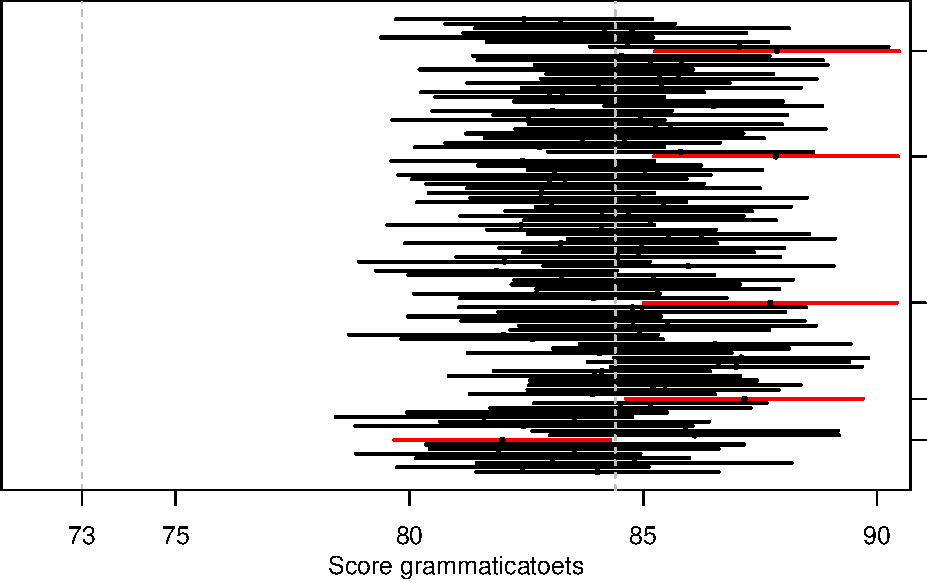
\includegraphics{KMS-NL_files/figure-latex/gramm2013CIs-1.pdf}
\caption{\label{fig:gramm2013CIs}95\%-Betrouwbaarheidsintervallen en steekproefgemiddelden, over 100 gesimuleerde steekproeven (n=34) uit een populatie met populatiegemiddelde 84.4, populatie-s.d. 8.4.}
\end{figure}

\hypertarget{sec:formules13-2}{%
\subsection{formules}\label{sec:formules13-2}}

Het tweezijdige betrouwbaarheidsinterval voor \(B\)\% betrouwbaarheid voor
een populatie-gemiddelde \(\overline{y}\) is
\begin{equation}
    \overline{y} \pm t^*_{N-1} \times \frac{s}{\sqrt{N}}
  \label{eq:t-onesampleCI}
\end{equation}

\hypertarget{spss-11}{%
\subsection{SPSS}\label{spss-11}}

\begin{verbatim}
Analyze > Descriptive Statistics > Explore...
\end{verbatim}

Selecteer afhankelijke variabele (sleep naar Dependent List paneel).\\
Kies knop \texttt{Statistics} en vink aan \texttt{Descriptives} met Confidence Interval
95\%.\\
Bevestig met \texttt{Continue} en met \texttt{OK}.\\
De uitvoer bevat meerdere beschrijvende statistische maten, waaronder nu
ook het 95\% betrouwbaarheidsinterval van het gemiddelde.

\hypertarget{jasp-1}{%
\subsection{JASP}\label{jasp-1}}

Hier komen JASP instructies.

\hypertarget{r-12}{%
\subsection{R}\label{r-12}}

R vermeldt het betrouwbaarheidsinterval van het gemiddelde (met een zelf
op te geven betrouwbaarheidsniveau) bij een \(t\)-toets. We voeren dus wederom een \(t\)-toets
uit en vinden het betrouwbaarheidsinterval van het gemiddelde in de
uitvoer.

\begin{Shaded}
\begin{Highlighting}[]
\KeywordTok{with}\NormalTok{( gramm2013, }\KeywordTok{t.test}\NormalTok{( score[opleiding}\OperatorTok{==}\StringTok{"TW"}\NormalTok{] ) )}
\end{Highlighting}
\end{Shaded}

\begin{verbatim}
## 
##  One Sample t-test
## 
## data:  score[opleiding == "TW"]
## t = 58.649, df = 33, p-value < 2.2e-16
## alternative hypothesis: true mean is not equal to 0
## 95 percent confidence interval:
##  81.48354 87.33999
## sample estimates:
## mean of x 
##  84.41176
\end{verbatim}

\hypertarget{sec:ttoets-onafh}{%
\section{\texorpdfstring{\(t\)-toets voor twee onafhankelijke steekproeven}{t-toets voor twee onafhankelijke steekproeven}}\label{sec:ttoets-onafh}}

De Student \(t\)-toets wordt toegepast om een verschil te kunnen onderzoeken tussen
de gemiddelde scores van twee onafhankelijke steekproeven, bv van
vergelijkbare jongens en meisjes. Op grond van de gemiddelden en de
standaarddeviaties van de twee steekproeven bepalen we de
toetsingsgrootheid \(t\). Als H0 waar is, dan is de waarde \(t=0\) het meest
waarschijnlijk. Naarmate het verschil tussen de twee gemiddelden groter
wordt, neemt \(t\) ook toe. Wederom verwerpen we H0 indien \(t>t^*\) voor
het gekozen significantieniveau \(\alpha\).

Als eerste voorbeeld nemen we een onderzoek naar de omvang van de
productieve woordenschat bij Zweedse meisjes en jongens van 18 maanden
oud \citep{Ande11}. We onderzoeken de veronderstelling dat de woordenschat
van meisjes verschilt van die van jongens, d.w.z. H1: \(\mu_m \ne \mu_j\).
We kunnen niet a priori aannemen dat een eventueel verschil slechts één
richting op kan gaan; we toetsen daarom tweezijdig, zoals al blijkt uit
H1. De bijbehorende nul-hypothese die we toetsen is H0: \(\mu_m = \mu_j\).
In dit onderzoek werd de woordenschat geschat op grond van vragenlijsten
aan de ouders van de kinderen in de steekproeven. Deelnemers waren
(ouders van) \(n_1=123\) meisjes en \(n_2=129\) jongens, allen 18 maanden
oud. Uit de resultaten blijkt dat de meisjes een gemiddelde woordenschat
hebben van \(\overline{x_1}=95\) woorden (\(s_1=82\)), en voor de jongens is
dat \(\overline{x_2}=85\) woorden (\(s_2=98\)). Met deze gegevens bepalen we
de toetsingsgrootheid \(t\) volgens formule
\eqref{eq:t-homoskedastic}, resulterend in \(t=0.88\) met 122 d.f. De
bijbehorende kritieke grenswaarde \(t^*\) zoeken we wederom op in
Bijlage~\ref{app:kritieketwaarden}. In de regel voor 100 d.f. (na
afronding naar beneden) vinden we \(t^*=1.984\) in de vierde kolom. Voor
tweezijdige toetsing moeten we de overschrijdingskans behorend bij deze
kolom verdubbelen (zie
§\ref{sec:ttoets-eenzijdigtweezijdig}), resulterend in \(p=.05\). De
gevonden toetsingsgrootheid \(t < t^*\), dus \(p>.05\). We besluiten om H0
\emph{niet} te verwerpen, en rapporteren dat als volgt:

\begin{quote}
De gemiddelde productieve woordenschat van Zweedse kinderen van 18
maanden oud verschilt nauwelijks tussen meisjes en jongens
(\(t(122)=0.88, p>.4\)). Meisjes produceren gemiddeld 95 verschillende
woorden (\(s=82\)), en jongens gemiddeld 85 verschillende woorden
(\(s=98\)).
\end{quote}

Als tweede voorbeeld nemen we een onderzoek naar het spreektempo van
twee groepen sprekers, nl. afkomstig uit het Westen (eerste groep) en
uit het Noorden (tweede groep) van Nederland. De spreeksnelheid wordt
hier uitgedrukt als de gemiddelde duur van een gesproken lettergreep,
gemiddeld over een interview van ca 15 minuten (zie voorbeeld \ref{ch:variantieanalyse}.1).
We onderzoeken H0: \(\mu_W = \mu_N\) met
tweezijdige toetsing. Uit de resultaten blijkt dat de westerlingen
(\(n=20\)) een gemiddelde lettergreepduur hebben van
\(\overline{x_W}=0.235\) s (\(s=0.028\)), en voor de noorderlingen (ook
\(n=20\)) is dat \(\overline{x_N}=0.269\) s (\(s=0.029\)). Met deze gegevens
bepalen we wederom de toetsingsgrootheid \(t\) volgens formule
\eqref{eq:t-homoskedastic}, resulterend in \(t=-3.76\) met 38 d.f. De
bijbehorende kritieke grenswaarde \(t^*\) zoeken we wederom op in
Bijlage~\ref{app:kritieketwaarden}. De juiste d.f. zijn niet in de tabel
vermeld, dus ronden we naar beneden af (d.i. in conservatieve richting)
naar 30 d.f. In die regel vinden we \(t^*=2.042\) in de vierde kolom. Voor
tweezijdige toetsing moeten we de overschrijdingskans behorend bij deze
kolom verdubbelen (zie
§\ref{sec:ttoets-eenzijdigtweezijdig}), resulterend in \(p=.05\). De
gevonden toetsingsgrootheid \(t < t^*\), dus \(p<.05\). We besluiten daarom
om H0 \emph{wel} te verwerpen, en rapporteren dat als volgt:

\begin{quote}
De gemiddelde duur van een lettergreep gesproken door een spreker uit
het westen van Nederland is \(0.235\) seconde (\(s=0.028\)). Dit is
significant korter dan bij sprekers uit het Noorden van Nederland
(\(\overline{x}=0.269\) s, \(s=0.029\)) (\(t(38)=-3.76, p<.05\)). In de
onderzochte opnames uit 1999 praten de sprekers uit het Westen dus
sneller dan die uit het Noorden van Nederland.
\end{quote}

\hypertarget{aannames}{%
\subsection{aannames}\label{aannames}}

De Student \(t\)-toets voor twee onafhankelijke steekproeven vereist vier aannames
(of assumpties) waaraan voldaan moet zijn, om de toets te mogen
gebruiken.

\begin{itemize}
\item
  De gegevens moeten gemeten zijn op intervalniveau (zie
  §\ref{sec:interval}).
\item
  Alle observaties moeten onafhankelijk van elkaar zijn.
\item
  De scores van beide groepen moeten normaal verdeeld zijn (zie
  §\ref{sec:isvarnormaalverdeeld}).
\end{itemize}

De variantie van de scores moet gelijk zijn in beide
steekproeven. Schending van deze aanname is ernstiger naarmate de twee
steekproeven meer in grootte verschillen. Het is daarom verstandig om te
werken met even grote, en liefst niet te kleine steekproeven. Als de
steekproeven even groot zijn dan is het schenden van deze aanname van
gelijke varianties niet zo ernstig.

\hypertarget{sec:ttoets-formules}{%
\subsection{formules}\label{sec:ttoets-formules}}

\hypertarget{toetsingsgrootheid}{%
\subsubsection{toetsingsgrootheid}\label{toetsingsgrootheid}}

Voor de berekening van de toetsingsgrootheid \(t\) zijn verschillende
formules in gebruik.

Indien de steekproeven ongeveer gelijke variantie hebben, dan gebruiken
we eerst de ``pooled standard deviation'' \(s_p\) als tussenstap. De beide
standaarddeviaties van de twee steekproeven worden daarin gewogen naar
hun steekproefomvang.
\begin{equation}
    s_p = \sqrt{ \frac{(n_1-1) s^2_1 + (n_2-1) s^2_2} {n_1+n_2-2} }
    \label{eq:sd-pooled}
\end{equation}
Vervolgens
\begin{equation}
  \label{eq:t-homoskedastic}
  t = \frac{ \overline{x_1}-\overline{x_2} } { s_p \sqrt{\frac{1}{n_1}+\frac{1}{n_2}} }
\end{equation}

Indien de steekproeven \emph{niet} gelijke variantie hebben, en de vierde
aanname hierboven dus is geschonden, dan wordt Welch's benadering
gebruikt:
\begin{equation}
  \label{eq:sd-WS}
  s_{\textrm{WS}} = \sqrt{\frac{s^2_1}{n_1}+\frac{s^2_2}{n_2} }
\end{equation}
Vervolgens
\begin{equation}
  \label{eq:t-WS}
  t = \frac{ \overline{x_1}-\overline{x_2} } { s_{\textrm{WS}} }
\end{equation}

\hypertarget{vrijheidsgraden}{%
\subsubsection{vrijheidsgraden}\label{vrijheidsgraden}}

Meestal wordt de uitgevoerd door een computerprogramma. Daarbij wordt
dan meestal de volgende benadering gebruikt van de vrijheidsgraden
(\(\nu\), zie §\ref{sec:ttoets-vrijheidsgraden}).
Eerst worden \(g_1=s^2_1/n_1\)
en \(g_2=s^2_2/n_2\) berekend. Het aantal vrijheidsgraden van \(t\) is dan
\begin{equation}
  \label{eq:df-WS}
  \nu_\textrm{WS} = 
        \frac {(g_1+g_2)^2} {g^2_1/(n_1-1) + g^2_2/(n_2-1)}
\end{equation}

Het aantal vrijheidsgraden volgens deze benadering heeft als liberale
bovengrens \((n_1+n_2-2)\), en als conservatieve ondergrens de kleinste
van \((n_1-1)\) of \((n_2-1)\). Je kunt dus ook altijd deze conservatieve
ondergrens gebruiken. Indien de twee groepen ongeveer dezelfde variantie
hebben (d.i. \(s_1 \approx s_2\)), dan kan je ook de liberale bovengrens
gebruiken.

Voor het tweede voorbeeld hierboven geeft de benadering van formule
\eqref{eq:df-WS} de
schatting van \(37.99 \approx 38\) d.f. De conservatieve ondergrens is
\(n_1-1 = n_2-1 = 19\). De liberale bovengrens is \(n_1+n_2 -2 = 38\). (In
de tabel met kritische waarden \(t*\), in
Bijlage~\ref{app:kritieketwaarden}, is het meestal raadzaam om de regel
te gebruiken met de eerstvolgende kleinere waarde voor het aantal
vrijheidsgraden.)

\hypertarget{sec:SPSS-ttoets-ongepaard}{%
\subsection{SPSS}\label{sec:SPSS-ttoets-ongepaard}}

Het tweede bovenstaande voorbeeld wordt hier uitgewerkt.

\begin{verbatim}
Analyze > Compare Means > Independent-Samples T Test
\end{verbatim}

Sleep de afhankelijke variabele \texttt{syldur} naar paneel Test Variable(s).
Sleep de onafhankelijke variabele \texttt{region} naar paneel Grouping
Variable. Definieer de twee groepen: waarde W voor regio groep 1 en
waarde N voor regrio groep 2. Bevestig met \texttt{Continue} en \texttt{OK}.

Zoals je hierboven kon zien, is de berekening van de \(t\)-toets afhankelijk van het
antwoord op de vraag of de standaarddeviaties van de twee groepen
ongeveer gelijk zijn. SPSS lost dat zeer onhandig op: je krijgt alle
relevante uitvoer te zien, en moet daar zelf een keuze uit maken.

\hypertarget{test-for-equality-of-variances}{%
\subsubsection{Test for equality of variances}\label{test-for-equality-of-variances}}

Met Levene's test wordt onderzocht H0: \(s^2_1 = s^2_2\), d.w.z. of de
varianties (en daarmee de standaarddeviaties) van de twee groepen gelijk
zijn. Als je een kleine waarde vindt voor de toetsingsgrootheid \(F\), en
een \(p>.05\), dan hoef je deze H0 niet te verwerpen. Je mag dan aannemen
dat de varianties gelijk zijn. Als je een grote waarde vindt voor \(F\),
met \(p<.05\), dan dien je deze H0 wel te verwerpen, en je mag niet
aannemen dat de varianties van de twee groepen gelijk zijn.

\hypertarget{test-for-equality-of-means}{%
\subsubsection{Test for equality of means}\label{test-for-equality-of-means}}

Afhankelijk van deze uitkomst van Levene's test moet je de eerste of de
tweede regel gebruiken van de uitvoer van de Independent-Samples Test
(een toets die onderzoekt of de gemiddelden van de twee groepen gelijk
zijn). In dit voorbeeld zijn de varianties ongeveer gelijk, zoals de
Levene's test ook aangeeft. We gebruiken dus de eerste regel van de
uitvoer, en rapporteren \(t(38)=-3.765, p=.001\).

\hypertarget{sec:R-ttoets-ongepaard}{%
\subsection{R}\label{sec:R-ttoets-ongepaard}}

\begin{Shaded}
\begin{Highlighting}[]
\KeywordTok{require}\NormalTok{(hqmisc)}
\KeywordTok{data}\NormalTok{(talkers)}
\KeywordTok{with}\NormalTok{(talkers, }\KeywordTok{t.test}\NormalTok{( syldur[region}\OperatorTok{==}\StringTok{"W"}\NormalTok{], syldur[region}\OperatorTok{==}\StringTok{"N"}\NormalTok{], }
            \DataTypeTok{paired=}\NormalTok{F, }\DataTypeTok{var.equal=}\NormalTok{T ) )}
\end{Highlighting}
\end{Shaded}

\begin{verbatim}
## 
##  Two Sample t-test
## 
## data:  syldur[region == "W"] and syldur[region == "N"]
## t = -3.7649, df = 38, p-value = 0.0005634
## alternative hypothesis: true difference in means is not equal to 0
## 95 percent confidence interval:
##  -0.0519895 -0.0156305
## sample estimates:
## mean of x mean of y 
##   0.23490   0.26871
\end{verbatim}

\hypertarget{sec:ttoets-gepaard}{%
\section{\texorpdfstring{\(t\)-toets voor gepaarde waarnemingen}{t-toets voor gepaarde waarnemingen}}\label{sec:ttoets-gepaard}}

De Student \(t\)-toets wordt ook toegepast om een verschil te onderzoeken tussen de
gemiddelden van twee afhankelijke of gepaarde waarnemingen. Daarvan is
sprake als we slechts één steekproef trekken (zie hoofdstuk
\ref{ch:steekproeftrekking}), en van de leden van deze steekproef
vervolgens twee observaties verzamelen, nl. één observatie onder elk van
beide condities. De twee observaties zijn dan gepaard, d.w.z. aan elkaar
gerelateerd, en deze observaties zijn dus niet onafhankelijk (want
afkomstig van hetzelfde lid van de steekproef). Eén van de assumpties
van de \(t\)-toets is daarmee geschonden.

Als voorbeeld nemen we een denkbeeldig onderzoek naar het gebruik van
\emph{U} of \emph{je} als aanspreekvorm op een website. De onderzoeker maakt twee
versies van een webpagina, de ene met \emph{U} en de andere met \emph{je}. Elke
respondent moet beide versies beoordelen op een schaal van 1 tot 10. (Om
redenen van validiteit wordt de volgorde van de twee versies gevarieerd
tussen respondenten; de volgorde waarin de pagina's beoordeeld zijn, kan
dus geen invloed hebben op de totaalscore per conditie.) In
Tabel~\ref{tab:data-uje-paired} zijn de oordelen van \(N=10\)
respondenten samengevat.

\begin{longtable}[]{@{}crrc@{}}
\caption{\label{tab:data-uje-paired} Fictieve oordelen over een webpagina met \emph{U} of \emph{je} als
aanspreekvorm, door \(N=10\) respondenten.}\tabularnewline
\toprule
id & conditie \emph{U} & conditie \emph{je} & \(D\)\tabularnewline
\midrule
\endfirsthead
\toprule
id & conditie \emph{U} & conditie \emph{je} & \(D\)\tabularnewline
\midrule
\endhead
1 & 8 & 9 & -1\tabularnewline
2 & 5 & 6 & -1\tabularnewline
3 & 6 & 9 & -3\tabularnewline
4 & 6 & 8 & -2\tabularnewline
5 & 5 & 8 & -3\tabularnewline
6 & 4 & 6 & -2\tabularnewline
7 & 4 & 8 & -4\tabularnewline
8 & 7 & 10 & -3\tabularnewline
9 & 7 & 9 & -2\tabularnewline
10 & 6 & 7 & -1\tabularnewline
& & & \(\overline{D}\)=-2.2\tabularnewline
\bottomrule
\end{longtable}

Het paar van observaties voor het \(i\)-de lid van de steekproef heeft een
verschil-score die we kunnen schrijven als:
\(D_i = x_{1i} - x_{2i}\) waarbij \(x_{1i}\) de score is van de afhankelijke
variabele is voor het \(i\)-de lid van de steekproef in conditie 1, en
\(x_{2i}\) de score voor het \(i\)-de lid voor conditie 2. Deze
verschilscore is ook vermeld in
Tabel~\ref{tab:data-uje-paired}.

Deze verschilscore \(D\) wordt vervolgens eigenlijk geanalyseerd met de
eerder besproken \(t\)-toets voor één enkele steekproef (zie
§\ref{sec:ttoets-onesample}), waarbij H0: \(\mu_D=0\), d.w.z. volgens H0 is er geen verschil
tussen condities. We berekenen het gemiddelde van de verschilscore,
\(\overline{D}\), en de standaarddeviatie van de verschilscore, \(s_{D}\),
op de gebruikelijke wijze (zie
§\ref{sec:standaarddeviatie}). We gebruiken dit gemiddelde en deze
standaarddeviatie om de toetsingsgrootheid \(t\) te berekenen, via formule
\eqref{eq:t-pairedsamples}, met \((N-1)\) vrijheidsgraden. Tenslotte
gebruiken we weer
Bijlage~\ref{app:kritieketwaarden} om de grenswaarde \(t^*\) te bepalen, en
daarmee de overschrijdingskans \(p\) voor de gevonden waarde van de
steekproefgrootheid \(t\) onder H0.

Voor het bovengenoemde voorbeeld met \emph{U} of \emph{je} als aanspreekvorm
vinden we aldus \(\overline{D}=-2.2\) en \(s_D=1.0\). Als we dit invullen in
formule~\eqref{eq:t-pairedsamples} vinden we \(t=-6.74\) met \(N-1=9\) d.f. De
bijbehorende kritieke grenswaarde \(t^*\) zoeken we wederom op in
Bijlage~\ref{app:kritieketwaarden}. Daarbij negeren we het teken van \(t\),
omdat de kansverdeling van \(t\) immers symmetrisch is. In de regel voor 9
d.f. vinden we \(t^*=4.297\) in de laatste kolom. Voor tweezijdige
toetsing moeten we de overschrijdingskans behorend bij deze kolom
verdubbelen (zie
§\ref{sec:ttoets-eenzijdigtweezijdig}), resulterend in \(p=.002\).
De gevonden toetsingsgrootheid \(t > t^*\), dus \(p<.002\). We besluiten om
H0 \emph{wel} te verwerpen, en rapporteren dat als volgt:

\begin{quote}
Het oordeel van \(N=10\) respondenten over de pagina met \emph{U} als
aanspreekvorm is gemiddeld 2.2 punten lager dan hun oordeel over de
vergelijkbare pagina met \emph{je} als aanspreekvorm; dit is een
significant verschil (\(t(9)=-6.74, p<.002\)).
\end{quote}

\hypertarget{aannames-1}{%
\subsection{aannames}\label{aannames-1}}

De \(t\)-toets voor gepaarde waarnemingen binnen een enkele steekproef vereist drie
aannames (assumpties) waaraan voldaan moet zijn, om deze toets te mogen
gebruiken.

\begin{itemize}
\item
  De gegevens moeten gemeten zijn op intervalniveau (zie
  §\ref{sec:interval}).
\item
  Alle \emph{paren} van observaties moeten onafhankelijk van elkaar
  zijn.
\item
  De \emph{verschilscores} \(D\) moeten normaal verdeeld zijn (zie
  §\ref{sec:isvarnormaalverdeeld}); als het aantal paren van
  waarnemingen in de steekproef echter groter is dan ca 30 dan is de \(t\)-toets
  doorgaans goed bruikbaar.
\end{itemize}

\hypertarget{sec:formules13-4}{%
\subsection{formules}\label{sec:formules13-4}}

\begin{equation}
  \label{eq:t-pairedsamples}
  t = \frac{ \overline{D}-\mu_D} { s_D } \times \sqrt{N}
\end{equation}

\hypertarget{sec:SPSS-ttoets-gepaard}{%
\subsection{SPSS}\label{sec:SPSS-ttoets-gepaard}}

De gegevens voor het bovenstaande voorbeeld zijn te vinden in bestand \texttt{data/ujedata.csv}.

\begin{verbatim}
Analyze > Compare Means > Paired-Samples T Test
\end{verbatim}

Sleep eerste afhankelijke variabele \texttt{cond.u} naar paneel Paired
Variables onder Variable1, en sleep tweede variabele \texttt{cond.je} naar
zelfde paneel onder Variable2. Bevestig met \texttt{OK}.

\hypertarget{sec:R-ttoets-gepaard}{%
\subsection{}\label{sec:R-ttoets-gepaard}}

De gegevens voor het bovenstaande voorbeeld zijn te vinden in bestand \texttt{data/ujedata.csv}.

\begin{Shaded}
\begin{Highlighting}[]
\NormalTok{ujedata \textless{}{-}}\StringTok{ }\KeywordTok{read.table}\NormalTok{( }\DataTypeTok{file=}\StringTok{"data/ujedata.csv"}\NormalTok{, }\DataTypeTok{header=}\OtherTok{TRUE}\NormalTok{, }\DataTypeTok{sep=}\StringTok{";"}\NormalTok{ )}
\KeywordTok{with}\NormalTok{(ujedata, }\KeywordTok{t.test}\NormalTok{( cond.u, cond.je, }\DataTypeTok{paired=}\OtherTok{TRUE}\NormalTok{ ) )}
\end{Highlighting}
\end{Shaded}

\begin{verbatim}
## 
##  Paired t-test
## 
## data:  cond.u and cond.je
## t = -6.7361, df = 9, p-value = 0.00008498
## alternative hypothesis: true difference in means is not equal to 0
## 95 percent confidence interval:
##  -2.938817 -1.461183
## sample estimates:
## mean of the differences 
##                    -2.2
\end{verbatim}

\hypertarget{sec:ttoets-effectgrootte}{%
\section{Effectgrootte}\label{sec:ttoets-effectgrootte}}

Tot nu toe zijn we vooral ingegaan op toetsing als een binaire
beslissing om H0 wel of niet te verwerpen, in het licht van de
observaties. Maar het is daarnaast ook van groot belang om te weten hoe
groot het geobserveerde effect eigenlijk is: de \emph{effectgrootte} (Eng.
`effect size', `ES') \citep{Cohen88, Thom02, Naka07}.

In formules \eqref{eq:t-onesample} en \eqref{eq:t-pairedsamples} komt tot uiting
dat \(t\) groter wordt,
naarmate het effect groter wordt, d.w.z. bij een groter verschil
\((\overline{x}-\mu)\) of \((\overline{x_1}-\overline{x_2})\) of
\((\overline{D}-\mu_D)\){]}, \emph{en/of} naarmate de steekproef groter wordt.
Kort gezegd \citep[ p.338, formule 11.10]{Rose08}:
\begin{equation}
  \label{eq:Rose08}
    \textrm{significance test} = 
    \textrm{size of effect} \times \textrm{size of study}
\end{equation}

Dat houdt
in dat een klein, en mogelijk triviaal effect, ook statistisch
significant kan zijn als de steekproef maar groot genoeg is. Omgekeerd
kan een heel groot effect goed vastgesteld worden op basis van een zeer
kleine steekproef.

\begin{center}\rule{0.5\linewidth}{0.5pt}\end{center}

\begin{quote}
\emph{Voorbeeld 13.2:}
In een onderzoek naar de levensduur van overleden 50+-ers uit Oostenrijk
en Denemarken \citep{Dobl99} bleek dat de levensduur verschilt met de
geboorteweek, vermoedelijk omdat babies uit ``zomerzwangerschappen''
gemiddeld iets gezonder zijn (of waren) dan die uit
``winterzwangerschappen''. In dit onderzoek waren de verschillen in
levensduur zeer gering (\(\pm 0.30\) jaar in Oostenrijk, \(\pm 0.15\) jaar
in Denemarken), maar het aantal observaties (overledenen) was zeer groot.
\end{quote}

\begin{quote}
Daarentegen is het verschil in lichaamslengte tussen dwergen (korter dan
1.5 m) en reuzen (langer dan 2.0 m) zo groot dat het verschil empirisch goed kan worden
vastgesteld op basis van slechts \(n=2\) in elke groep.
\end{quote}

\begin{center}\rule{0.5\linewidth}{0.5pt}\end{center}

In ons onderzoek zijn we vooral geïnteresseerd in belangrijke
verschillen, d.w.z. doorgaans grote verschillen. We moeten beseffen dat
onderzoek ook kosten met zich meebrengt in termen van geld, tijd,
inspanning, privacy, en verlies van onbevangenheid voor ander onderzoek
(zie hoofdstuk
\ref{ch:integriteit}). We willen dus niet nodeloos onderzoek doen
naar triviale effecten. Een onderzoeker dient daarom vooraf te bepalen
wat het kleinste effect is dat hij/zij wil kunnen opsporen, bv. 1 punt
verschil in de score van de grammaticatoets. Verschillen kleiner dan 1
punt worden dan beschouwd als triviaal, en verschillen groter dan 1 punt
als potentieel interessant.

Ook is het van belang om de gevonden effectgrootte te vermelden bij de
resultaten van een onderzoek, om lezers en latere onderzoekers van
dienst te zijn. In sommige wetenschappelijke tijdschriften is het zelfs
verplicht om effectgrootte te rapporteren. Dat kan overigens ook in de
vorm van een betrouwbaarheidsinterval van het gemiddelde
(zie~\ref{sec:t-betrouwbaarheidsinterval-gemiddelde}), omdat we deze
betrouwbaarheidsintervallen en effectgroottes in elkaar kunnen
omrekenen.

De ruwe effectgrootte is eenvoudigweg het verschil \(D\) in gemiddelden
tussen twee groepen, of tussen twee condities, uitgedrukt in eenheden
van de ruwe score. In §\ref{sec:ttoets-onafh} vonden we zo een verschil in woordenschat
van \(D=95-85=10\) tussen jongens en meisjes.

Meestal gebruiken we echter de gestandaardiseerde effectgrootte (zie
formules hieronder), waarbij we rekening houden met de spreiding in de
observaties, bijv in de vorm van ``pooled standard deviation'' \(s_p\) \footnote{In dit geval gebruiken we \(s_p = \sqrt{ \frac{122\times82^2+128\times98^2} {122+128} } = 90.5\), zie formules \eqref{eq:sd-pooled} en \eqref{eq:d-homoskedastic}.}.
We vinden zo een gestandaardiseerde effectgrootte van
\begin{equation}
  \label{eq:d-standardized}
    d = \frac{ \overline{x_1}-\overline{x_2} } {s_p} = \frac{10}{90.5} = 0.11
\end{equation}
In het eerste voorbeeld hierboven is de gestandaardiseerde effectgrootte
van het verschil in woordenschat tussen meisjes en jongens dus 0.11. In
dit geval is het verschil tussen de groepen gering ten opzichte van de
spreiding binnen de groepen --- de kans dat een willekeurig gekozen
meisje een grotere woordenschat heeft dan een willekeurig gekozen
jongen, is slechts 0.53 \citep{McGraw92}, en dat is nauwelijks beter dan de
kans van 0.50 die we verwachten volgens H0. Dat dit zeer kleine effect
niet significant is (zie §\ref{sec:ttoets-onafh}) wekt dan ook geen verbazing.
We zouden de
effectgrootte en significantie als volgt kunnen rapporteren:

\begin{quote}
De gemiddelde productieve woordenschat van Zweedse kinderen van 18
maanden oud verschilt nauwelijks tussen meisjes en jongens. Meisjes
produceren gemiddeld 95 verschillende woorden (\(s=82\)), en jongens
gemiddeld 85 verschillende woorden (\(s=98\)). Het verschil is zeer
klein (\(d=0.11)\) en niet significant (\(t(122)=0.88, p>.4\)).
\end{quote}

In het tweede voorbeeld hierboven is de gestandaardiseerde effectgrootte
van het verschil in duren van lettergrepen ongeveer
\((0.235-0.269)/0.029 \approx 1.15\). Dit relatief grote effect kunnen we
als volgt rapporteren:

\begin{quote}
De gemiddelde duur van een lettergreep gesproken door een spreker uit
het westen van Nederland is \(0.235\) seconde (\(s=0.028\)). Dit is
aanzienlijk korter dan bij sprekers uit het Noorden van Nederland
(\(\overline{x}=0.269\) s, \(s=0.029\)). Het verschil is ca. 10\%; dit
verschil is zeer groot (\(d=-1.15\)) en significant
(\(t(38)=-3.76, p<.05\)). In de onderzochte opnames uit 1999 praten de
sprekers uit het Westen dus aanzienlijk sneller dan die uit het
Noorden van Nederland.
\end{quote}

Als \(d\) ligt rond 0.2 spreken we van een klein effect. Een effectgrootte
\(d\) rond 0.5 noemen we een middelmatig (medium) effect, en een \(d\) rond
0.8 of groter noemen we een groot effect \citep{Cohen88, Rose08}.

\begin{figure}
\centering
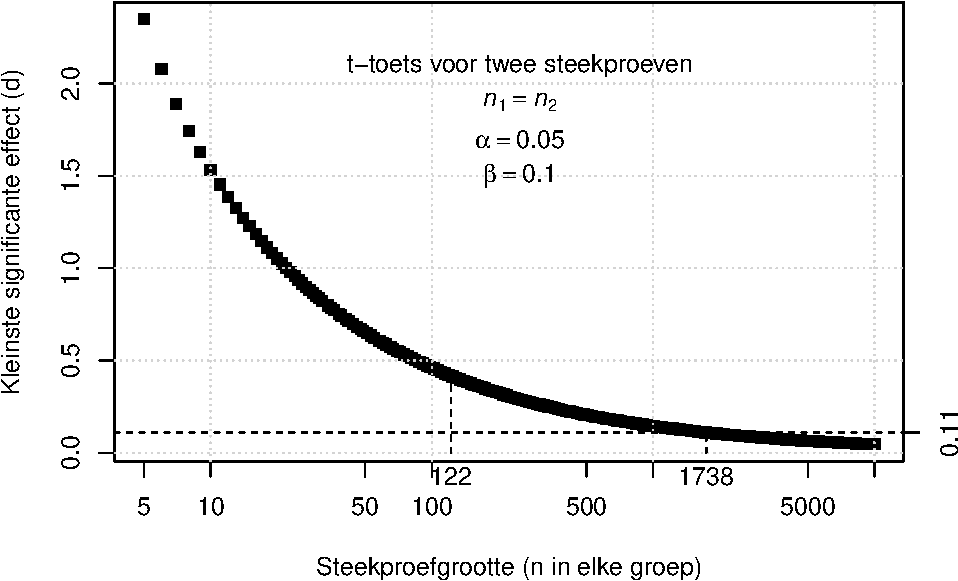
\includegraphics{KMS-NL_files/figure-latex/kleinstesignifverschil-1.pdf}
\caption{\label{fig:kleinstesignifverschil}Relatie tussen de steekproefgrootte en het kleinste effect (d) dat significant is volgens een \emph{t}-toets voor ongepaarde, onafhankelijke waarnemingen, met foutkansen alpha=.05 en beta=.10.}
\end{figure}

\begin{center}\rule{0.5\linewidth}{0.5pt}\end{center}

\begin{quote}
\emph{Voorbeeld 13.3:}
Kijk nog eens naar formule
\eqref{eq:Rose08}
en naar Figuur~\ref{fig:kleinstesignifverschil} die de relatie tussen
steekproefgrootte en effectgrootte illustreert. Met een
steekproefgrootte van \(n_1=122\) kunnen we alleen een effect van \(d=0.42\)
of groter opsporen, met voldoende kleine kansen op fouten van Typen I en
II (\(\alpha=.05, \beta=.10\)). Om het zeer kleine effect van \(d=0.11\) op
te sporen, met dezelfde kleine foutkansen \(\alpha\) en \(\beta\), zouden er
steekproeven van tenminste 1738 meisjes en 1738 jongens nodig zijn.
\end{quote}

\begin{center}\rule{0.5\linewidth}{0.5pt}\end{center}

We kunnen de effectgrootte ook uitdrukken als de waarschijnlijkheid dat
een verschil in de voorspelde richting optreedt, voor een willekeurig
gekozen element uit de populatie
(formules~\eqref{eq:d-onesample} en \eqref{eq:d-paired}),
of (indien van toepassing) voor twee
willekeurig en onafhankelijk gekozen elementen uit de twee populaties
(formule~\eqref{eq:d-homoskedastic}) \citep{McGraw92}. Laten we nog eens
terugkeren naar de grammaticatoets van de studenten Taalwetenschap
(§\ref{sec:ttoets-onesample}). Het effect dat we vonden is niet
alleen significant maar ook groot. In termen van waarschijnlijkheid
uitgedrukt: de kans dat een willekeurige student Taalwetenschap een
score behaalt groter dan \(\mu_0=73\) is 0.91. (En een willekeurig gekozen
student Taalwetenschap heeft dus nog 9\% kans om lager te scoren dan het
veronderstelde populatie-gemiddelde van 73.)

Voor de fictieve oordelen over de webpagina's met \emph{U} of \emph{je} (zie
Tabel~\ref{tab:data-uje-paired}) vinden we een gestandaardiseerde
effectgrootte van
\[d = \frac{ \overline{D}-\mu_D} {s_D} = \frac{ -2.20-0 } {1.03} = -2.13\]
Dat dit extreem grote effect inderdaad significant is, wekt dan ook geen
verbazing. We kunnen dat als volgt rapporteren:

\begin{quote}
De oordelen van \(N=10\) respondenten over de pagina's met \emph{U} of \emph{je}
als aanspreekvorm verschillen significant, met gemiddeld \(-2.2\) punten
verschil. Dit verschil heeft een 95\% betrouwbaarheidsinterval van
\(-2.9\) tot \(-1.5\) en een geschatte gestandaardiseerde effectgrootte
\(d=-2.13\); de kans dat een willekeurig gekozen respondent de
\emph{je}-versie hoger beoordeelt dan de \emph{U}-versie is \(p=.98\).
\end{quote}

\hypertarget{sec:formules13-5}{%
\subsection{formules}\label{sec:formules13-5}}

Voor een enkele steekproef:
\begin{equation}
   \label{eq:d-onesample}
  d = \frac{\overline{x}-\mu}{s}
\end{equation}
waarbij \(s\) de standaarddeviatie \(s\)
van de score \(x\) voorstelt.

Voor twee onafhankelijke steekproeven (zie
formule~\eqref{eq:sd-pooled}):
\begin{equation}
  \label{eq:d-homoskedastic}
  d = \frac{ \overline{x_1}-\overline{x_2} } { s_p }
\end{equation}

Voor gepaarde waarnemingen:
\begin{equation}
  \label{eq:d-paired}
  d = \frac{ \overline{x_1}-\overline{x_2} } { s_D }
\end{equation}
waarbij \(s_D\) de
standaarddeviatie is van het verschil \(D\) volgens
formule~\eqref{eq:d-paired}.

\hypertarget{spss-13-2}{%
\subsection{SPSS}\label{spss-13-2}}

In SPSS kunnen we de effectgrootte meestal het makkelijkste met de hand
uitrekenen.

Voor een enkele steekproef
(formule~\eqref{eq:d-onesample}) kunnen we de effectgrootte eenvoudig
uitrekenen uit het gemiddelde en de standaarddeviatie, rekening houdend
met de waarde \(\mu\) waartegen we toetsen.

\begin{verbatim}
Analyze > Descriptive Statistics > Descriptives...
\end{verbatim}

Kies de knop \texttt{Options} en zorg dat \texttt{Mean} en \texttt{Std.deviation} zijn
aangevinkt. In de uitvoer staan vervolgens de benodigde gegevens:\\
\(d = (84.41 - 73) / 8.392 = 1.36\), een zeer groot effect.

Voor ongepaarde, onafhankelijke waarnemingen kunnen we eveneens de
effectgrootte het beste met de hand uitrekenen op basis van de
gemiddelden, standaarddeviaties, en omvang van de twee steekproeven,
gebruik makend van
formules~\eqref{eq:sd-pooled} en
\eqref{eq:d-homoskedastic} hierboven.

Voor een enkele steekproef met twee gepaarde observaties
(formule~\eqref{eq:d-paired}) kunnen we de effectgrootte weer eenvoudiger
uitrekenen uit het gemiddelde en de standaarddeviatie van het verschil.
De gegevens staan in de uitvoer van de paarsgewijze \(t\)-toets
(§\ref{sec:SPSS-ttoets-gepaard}), respectievelijk als \texttt{Mean} en
\texttt{Std.Deviation}:\\
\(d = -2.200 / 1.033 = 2.130\), een super groot effect.

\hypertarget{r-13}{%
\subsection{R}\label{r-13}}

In R is het wat makkelijker om de effectgrootte te laten uitrekenen.

Voor een enkele steekproef
(formule~\eqref{eq:d-onesample}):\\

\begin{Shaded}
\begin{Highlighting}[]
\NormalTok{gramm2013 \textless{}{-}}\StringTok{ }\KeywordTok{read.csv}\NormalTok{( }\DataTypeTok{file=}\StringTok{"data/grammaticatoets2013.csv"}\NormalTok{,}\DataTypeTok{header=}\NormalTok{F)}
\KeywordTok{dimnames}\NormalTok{(gramm2013)[[}\DecValTok{2}\NormalTok{]] \textless{}{-}}\StringTok{ }\KeywordTok{c}\NormalTok{(}\StringTok{"score"}\NormalTok{,}\StringTok{"opleiding"}\NormalTok{)}
\KeywordTok{with}\NormalTok{(gramm2013, score[opleiding}\OperatorTok{==}\StringTok{"TW"}\NormalTok{]) {-}\textgreater{}}\StringTok{ }\NormalTok{score.TW }\CommentTok{\# hulpvariabele}
\NormalTok{( }\KeywordTok{mean}\NormalTok{(score.TW)}\OperatorTok{{-}}\DecValTok{73}\NormalTok{ ) }\OperatorTok{/}\StringTok{ }\KeywordTok{sd}\NormalTok{(score.TW) }
\end{Highlighting}
\end{Shaded}

\begin{verbatim}
## [1] 1.359783
\end{verbatim}

De kans op een score groter dan het populatiegemiddelde (de toetswaarde) \texttt{73} voor een willekeurige student Taalwetenschap (waarvan we aannemen dat \(\mu=84.4\) en \(s=8.4\)):

\begin{Shaded}
\begin{Highlighting}[]
\DecValTok{1} \OperatorTok{{-}}\StringTok{ }\KeywordTok{pnorm}\NormalTok{( }\DecValTok{73}\NormalTok{, }\DataTypeTok{mean=}\FloatTok{84.4}\NormalTok{, }\DataTypeTok{sd=}\FloatTok{8.4}\NormalTok{ ) }
\end{Highlighting}
\end{Shaded}

\begin{verbatim}
## [1] 0.9126321
\end{verbatim}

Voor ongepaarde, onafhankelijke waarnemingen kunnen we het kleinste
significante effect uitrekenen (zie ook
Fig.~\ref{fig:kleinstesignifverschil}); daarvoor gebruiken we de functie \texttt{power.t.test}. (Deze functie is ook gebruikt om Fig.\ref{fig:kleinstesignifverschil} te construeren.)
Je moet bij die functie de gewenste \texttt{power} als
argument opgeven (power = \(1-\beta\); zie
§\ref{sec:power-inleiding}).

\begin{Shaded}
\begin{Highlighting}[]
\KeywordTok{power.t.test}\NormalTok{( }\DataTypeTok{n=}\DecValTok{122}\NormalTok{, }\DataTypeTok{sig=}\NormalTok{.}\DecValTok{05}\NormalTok{, }\DataTypeTok{power=}\NormalTok{.}\DecValTok{90}\NormalTok{, }\DataTypeTok{type=}\StringTok{"two.sample"}\NormalTok{ )}
\end{Highlighting}
\end{Shaded}

\begin{verbatim}
## 
##      Two-sample t test power calculation 
## 
##               n = 122
##           delta = 0.4166921
##              sd = 1
##       sig.level = 0.05
##           power = 0.9
##     alternative = two.sided
## 
## NOTE: n is number in *each* group
\end{verbatim}

In de uitvoer staat bij \texttt{delta} het kleinste significante effect aangegeven; zie ook Voorbeeld 13.3 hierboven.

Voor een enkele steekproef met twee gepaarde observaties
(formule~\eqref{eq:d-paired}):

\begin{Shaded}
\begin{Highlighting}[]
\NormalTok{ujedata \textless{}{-}}\StringTok{ }\KeywordTok{read.table}\NormalTok{( }\DataTypeTok{file=}\StringTok{"data/ujedata.csv"}\NormalTok{, }\DataTypeTok{header=}\OtherTok{TRUE}\NormalTok{, }\DataTypeTok{sep=}\StringTok{";"}\NormalTok{ )}
\KeywordTok{with}\NormalTok{( ujedata, }\KeywordTok{mean}\NormalTok{(cond.u}\OperatorTok{{-}}\NormalTok{cond.je) }\OperatorTok{/}\StringTok{ }\KeywordTok{sd}\NormalTok{(cond.u}\OperatorTok{{-}}\NormalTok{cond.je) )}
\end{Highlighting}
\end{Shaded}

\begin{verbatim}
## [1] -2.130141
\end{verbatim}

\hypertarget{betrouwbaarheidsinterval-van-de-effectgrootte}{%
\subsection{Betrouwbaarheidsinterval van de effectgrootte}\label{betrouwbaarheidsinterval-van-de-effectgrootte}}

We hebben al eerder gezien
(§\ref{sec:betrouwbaarheidsinterval-gemiddelde} en §\ref{sec:t-betrouwbaarheidsinterval-gemiddelde})
dat we een kenmerk
of parameter van de populatie kunnen schatten op basis van een kenmerk
van een steekproef. Zo hebben we het onbekende populatiegemiddelde \(\mu\)
geschat op basis van het geobserveerde steekproefgemiddelde
\(\overline{x}\). Bij die schatting hoort wel een bepaalde mate van
onzekerheid of betrouwbaarheid: misschien verschilt de onbekende
parameter in de populatie enigszins van het steekproefkenmerk, dat we
als schatter gebruiken, ten gevolge van toevallige variaties in de
steekproef. De (on)zekerheid of (on)betrouwbaarheid wordt uitgedrukt als
een betrouwbaarheidsinterval van het geschatte kenmerk. We weten dan met
een bepaalde betrouwbaarheid (meestal 95\%) dat de onbekende parameter
binnen dat interval zal liggen
(§\ref{sec:betrouwbaarheidsinterval-gemiddelde} en §\ref{sec:t-betrouwbaarheidsinterval-gemiddelde}).

Deze redenatie nu geldt niet alleen voor de gemiddelde score, of voor de
mediaan of voor de variantie, maar evenzo voor de effectgrootte. Ook de
effectgrootte is immers een onbekende parameter uit de populatie, die we
proberen te schatten op grond van een beperkte steekproef. Voor de
fictieve oordelen over de webpagina's met \emph{U} of \emph{je} (zie
Tabel~\ref{tab:data-uje-paired}) vonden we een gestandaardiseerde
effectgrootte van \(d=-2.13\). Dit is een schatting van de onbekende
effectgrootte (d.i. van de sterkte van de voorkeur voor de \emph{je}-variant)
in de populatie van beoordelaars, op basis van een steekproef van \(n=10\)
beoordelaars. We kunnen ook hier de betrouwbaarheid van deze schatting
aangeven, in de vorm van een \emph{betrouwbaarheidsinterval} rondom de
geobserveerde effectgrootte \(d=-2.13\).

Het betrouwbaarheidsinterval van de effectgrootte is wel wat lastig vast
te stellen \citep{Naka07, Chen15}. We illustreren het hier op simpele wijze
voor het simpelste geval, nl. dat van de \(t\)-toets voor een enkele steekproef,
c.q. voor twee gepaarde observaties. We hebben hiervoor twee elementen
nodig: ten eerste de effectgrootte uitgedrukt als correlatie \citep[ p.359, formule 12.1]{Rose08}, \[r = \sqrt{ \frac{t^2}{t^2+\textrm{df}} }\] en
ten tweede de standaardfout van de effectgrootte \(d\) \citep[ p.600,
formule 18]{Naka07}:
\begin{equation}
  \label{eq:d-paired-se}
    \textrm{se}_d = \sqrt{ \frac{2(1-r)}{n} + \frac{d^2}{2(n-1)} }
\end{equation}
In
ons eerdere voorbeeld van de \(n=10\) gepaarde oordelen over een webpagina
met \emph{U} of \emph{je} als aanspreekvorm vonden we \(d=-2.13\). We vinden ook dat
\(r=.9135\). Met deze gegevens vinden we \(\textrm{se}_d = 0.519\) via
formule~\eqref{eq:d-paired-se}.

Hiermee bepalen we vervolgens het betrouwbaarheidsinterval voor de
effectgrootte:
\begin{equation}
   \label{eq:d-paired-CI}
    d \pm t^*_{n-1} \times \textrm{se}_d 
\end{equation}
(zie de overeenkomstige
formule~\eqref{eq:t-onesampleCI}).
Na invullen van \(t^*_9=2.262\) (zie
Bijlage~\ref{app:kritieketwaarden}) en \(\textrm{se}_d = 0.519\) vinden we
uiteindelijk een 95\%-betrouwbaarheidsinterval van \((-3.30,-0.96)\). We
weten dus met 95\% betrouwbaarheid dat de onbekende effectgrootte in de
populatie ergens binnen dit interval ligt, en dus ook dat die kleiner is
dan nul. Op grond van die laatste overweging kunnen we H0 verwerpen.
Maar: we weten nu niet alleen \emph{dat} de voorkeur afwijkt van nul, maar
ook \emph{in welke mate} de (gestandaardiseerde) voorkeur afwijkt van nul,
d.w.z. hoe sterk de voorkeur voor de \emph{je}-versie is. Deze nieuwe kennis
over de mate of grootte van het effect is vaak nuttiger en interessanter
dan de binaire beslissing of er wel of niet een effect is (H0 wel of
niet verwerpen) \citep{Cumm12}.

\hypertarget{ch:power}{%
\chapter{Power}\label{ch:power}}

\hypertarget{sec:power-inleiding}{%
\section{Inleiding}\label{sec:power-inleiding}}

Bij statistische toetsing van H0 bepalen we de kans \(P\) op de
geobserveerde verschillen of effecten (of op nog grotere verschillen of
effecten dan geobserveerd) indien H0 waar zou zijn, en dus indien het
geobserveerde verschil louter aan het toeval toegeschreven moet worden
(zie §\ref{sec:empirischecyclus} en
Hoofdstuk~\ref{ch:toetsing}). Als die kans \(P\) zeer klein is, dan hebben we
dus resultaten gevonden die zeer onwaarschijnlijk zijn als H0 waar zou
zijn. We concluderen dan dat H0 vermoedelijk \emph{niet waar} is en we
verwerpen daarom H0. Het gevonden verschil of effect noemen we dan
``significant'' (Latijn: `betekenis makend'). Er is echter wel een kans,
\(P\), dat het gevonden verschil toch een toevalstreffer was, en dat we
door H0 te verwerpen een fout van Type-I maken (d.w.z. H0 ten onrechte
verwerpen, zie
§\ref{sec:toetsing-inleiding}). Omdat we een bepaald
significantieniveau \(\alpha\) hanteren waarmee we \(P\) vergelijken, is
deze \(\alpha\) dus ook de kans dat we een Type-I-fout maken.

Minstens even belangrijk, echter, is de omgekeerde fout om H0 ten
onrechte \emph{niet} te verwerpen, een Type-II-fout. Voorbeelden van deze
fouten zijn: een verdachte niet veroordelen ook al is hij schuldig, een
`spam' mail-bericht doorlaten naar mijn mailbox, een patiënt onderzoeken
en diens ziekte toch niet opmerken, concluderen dat vogels zwijgen
hoewel ze toch zingen
(voorbeeld~13.1), of ten onrechte concluderen dat twee
groepen niet verschillen hoewel er wel een belangrijk verschil bestaat
tussen de twee groepen. De kans op een Type-II-fout wordt aangeduid met
het symbool \(\beta\).

Als H0 in werkelijkheid niet waar is (er is een verschil, het bericht is
`spam', de vogels zingen, enz), dan dient H0 dus verworpen te worden, en
dient \(\beta\) dus zo klein mogelijk te zijn. De kans om H0 dan \emph{terecht}
te verwerpen is dan \((1-\beta)\) (zie complementregel \eqref{eq:complementregel});
deze kans \((1-\beta)\) wordt de \emph{power}
genoemd. Power is op te vatten als \textbf{de kans voor de onderzoeker om gelijk
te \emph{krijgen}} (H0 wordt verworpen) \textbf{als zij ook gelijk \emph{heeft}} (H0 is onwaar).

De kansen op fouten van Type-I en Type-II moeten goed tegen elkaar
afgewogen worden. In veel onderzoek worden als overschrijdingskansen
gehanteerd \(\alpha=.05\) (significantieniveau) en \(\beta=.20\)
(power=\(.80\)). Hiermee wordt een impliciete afweging gemaakt dat een
Type-I-fout \(4\times\) zo ernstig is als een Type-II-fout. Voor sommige
onderzoeken zou dat gerechtvaardigd kunnen zijn, maar het is ook goed
denkbaar dat onder bepaalde omstandigheden een Type-II-fout eigenlijk
nog ernstiger is dan een Type-I-fout. Als we beide typen fouten min of
meer even ernstig vinden, dan zouden we dus moeten streven naar een
kleinere \(\beta\) en grotere power \citep{Rose08}.

De power van een onderzoek hangt af van drie factoren: (i) de
effectgrootte \(d\), die zelf weer afhankelijk is van het gemeten verschil
\(D\) en van de variatie \(s\) in de observaties
(formule \eqref{eq:d-standardized}), (ii) de steekproefgrootte \(N\), en (iii)
het significantieniveau \(\alpha\). In de volgende paragrafen zullen we
deze factoren afzonderlijk bespreken, waarbij we de andere twee factoren
zoveel mogelijk constant houden. Bij deze bespreking gebruiken we
afbeeldingen van de berekende power
(Figuren~\ref{fig:powercontours-alpha01} en
\ref{fig:powercontours-alpha05}). De afgebeelde power-contouren
zijn specifiek voor een \emph{t}-toets voor onafhankelijke steekproeven
(§\ref{sec:ttoets-onafh}) met tweezijdige toetsing. De hieronder
besproken verbanden treden echter ook op bij andere statistische
toetsen.

\begin{figure}
\centering
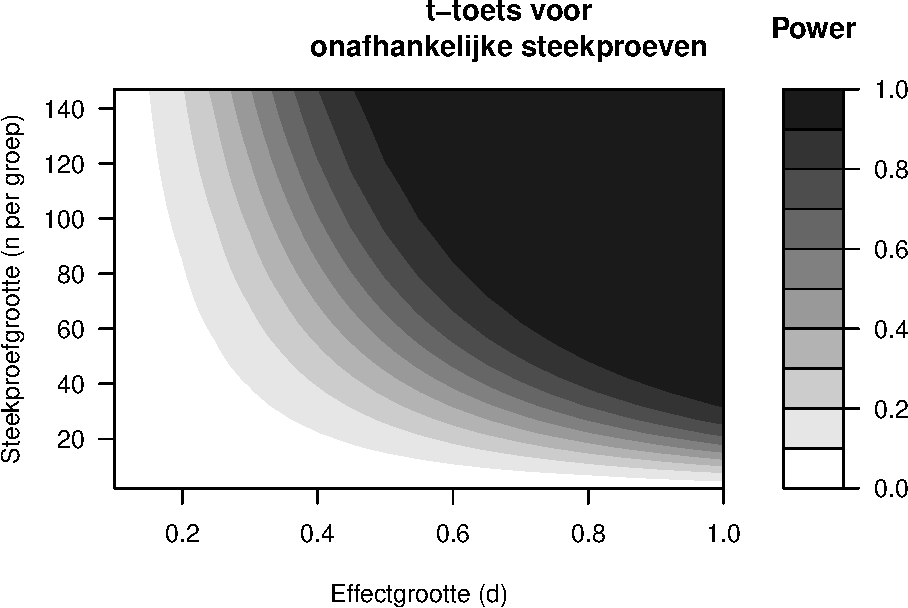
\includegraphics{KMS-NL_files/figure-latex/powercontours-alpha01-1.pdf}
\caption{\label{fig:powercontours-alpha01}Power uitgedrukt in contouren (zie schaalverdeling), afhankelijk van de gestandaardiseerde effectgrootte (d) en de steekproefgrootte (n), volgens een tweezijdige t-toets voor ongepaarde, onafhankelijke waarnemingen, met significantieniveau alpha=.01.}
\end{figure}

\begin{figure}
\centering
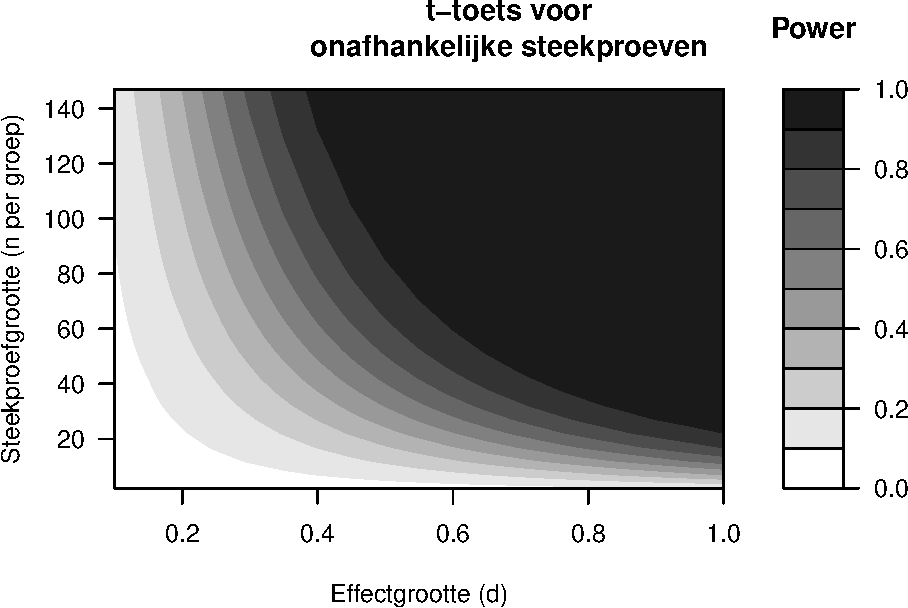
\includegraphics{KMS-NL_files/figure-latex/powercontours-alpha05-1.pdf}
\caption{\label{fig:powercontours-alpha05}Power uitgedrukt in contouren (zie schaalverdeling), afhankelijk van de gestandaardiseerde effectgrootte (d) en de steekproefgrootte (n), volgens een tweezijdige t-toets voor ongepaarde, onafhankelijke waarnemingen, met significantieniveau alpha=.05.}
\end{figure}

\hypertarget{sec:effectgrootte-power}{%
\section{Verband tussen effectgrootte en power}\label{sec:effectgrootte-power}}

De twee figuren~\ref{fig:powercontours-alpha01} en
\ref{fig:powercontours-alpha05} laten zien dat in het algemeen de
power toeneemt, naarmate het te toetsen effect groter is (meer naar
rechts in elke figuur). Dat is ook niet verwonderlijk: een groter effect
heeft een grotere kans om opgespoord te worden in een statistische toets
dan een kleiner effect, onder dezelfde omstandigheden. Een middelmatig
groot effect van \(d=.5\) heeft, bij \(n=30\) observaties in elke groep,
slechts een kans van \(.48\) om opgespoord te worden (als \(\alpha=.05\), Figuur \ref{fig:powercontours-alpha05}). Op basis van een
onderzoek met \(n=30\) observaties per groep is het dus eigenlijk een
grote gok of een onderzoeker zo'n effect (met \(d=.5\)) wel zal opsporen,
en H0 zal verwerpen. Anders gezegd, de kans op een Type-I-fout is
weliswaar veilig laag (\(\alpha=.05\)) maar de kans op een Type-II-fout is
meer dan \(10\times\) zo groot, en daarmee gevaarlijk hoog (\(\beta=.52\)) \citep[Ch.12]{Rose08}.

Een groter effect heeft een grotere kans om opgespoord te worden. Een
groter effect van \(d=.8\), bijvoorbeeld, resulteert in een power van
\(.86\) bij dezelfde toetsing. De kans op een Type-II-fout \(\beta=.14\) is
weliswaar ook hier groter dan de kans op een Type-I-fout, maar de
verhouding \(\beta/\alpha\) is aanzienlijk minder scheef.

Als onderzoeker hebben we alleen indirect invloed op de effectgrootte.
We hebben uiteraard geen invloed op het ware ruwe verschil \(D\) in de
populatie. Voor de power is echter niet dat ruwe verschil \(D\) van
belang, maar het gestandaardiseerde verschil \(d=D/s\)
(§\ref{sec:ttoets-effectgrootte}). Dus als we zorgen dat de
standaarddeviatie \(s\) op enige wijze kleiner wordt, dan wordt daarmee
\(d\) groter, en dan wordt daarmee weer de power groter
(figuren~\ref{fig:powercontours-alpha01} en \ref{fig:powercontours-alpha05}),
en dan hebben we dus meer kans
om een bestaand effect daadwerkelijk op te sporen! Vanwege dat doel
streven onderzoekers er altijd naar om storende invloeden van allerlei
andere factoren zoveel mogelijk te neutraliseren. Die storende invloeden
zorgen immers voor extra variabiliteit in de observaties, en daarmee
voor een lagere power bij de statistische toetsing.

In een goed opgezet onderzoek willen we vooraf al bepalen wat de power
zal zijn, en hoe groot de steekproef dient te zijn (zie hierna).
Daarvoor hebben we een schatting nodig van de kleinste effectgrootte \(d\)
die we nog willen opsporen
(§\ref{sec:ttoets-effectgrootte}) \citep{Quene10}. Om de effectgrootte te
schatten, is ten eerste een schatting nodig van het ruwe verschil \(D\)
tussen de groepen of condities. Ten tweede is er een schatting nodig van
de variabiliteit \(s\) in de observaties. Die schattingen zijn meestal af
te leiden uit eerdere publicaties, waarin doorgaans ook de
standaarddeviatie \(s\) wordt gerapporteerd. Als er geen eerdere
onderzoeksrapporten beschikbaar zijn, dan kan \(s\) grofweg geschat worden
uit enkele informele `pilot'-observaties. Neem daarvan het verschil
tussen de hoogste en de laagste (bereik of `range'), deel dit bereik
door 4, en gebruik de uitkomst daarvan als grove schatting voor \(s\)
\citep{PD08}.

\hypertarget{sec:steekproefgrootte-power}{%
\section{Verband tussen steekproefgrootte en power}\label{sec:steekproefgrootte-power}}

Het verband tussen de steekproefgrootte \(N\) en de power van een
onderzoek wordt geïllustreerd in
Figuur~\ref{fig:powercontours-alpha01} voor een streng
significantieniveau \(\alpha=.01\), en in
Figuur~\ref{fig:powercontours-alpha05} voor het meest gebruikte
significantieniveau \(\alpha=.05\). De figuren laten zien dat in het
algemeen de power toeneemt, naarmate de steekproef groter wordt (meer
naar boven). De toename is steiler (power neemt sneller toe) bij grotere
effecten (rechterkant) dan bij kleinere effecten (linkerkant). Anders gezegd: bij
kleine effecten is de steekproef eigenlijk bijna altijd te klein om deze
kleine effecten met voldoende power te kunnen opsporen. We zagen dat al
eerder in voorbeeld~13.3 (Hoofdstuk \ref{ch:toetsing}).

De twee figuren~\ref{fig:powercontours-alpha01} en
\ref{fig:powercontours-alpha05} zijn gebaseerd op de vergelijking tussen twee groepen die even groot zijn, elk met precies de helft van de observaties (\(n_1=n_2=N/2\)). Dat is ook het meest efficiënt.
De power is gebaseerd op het \emph{harmonisch gemiddelde} van \(n_1\) en \(n_2\) (zie §\ref{sec:harmonischgemiddelde}), en dat harmonisch gemiddelde is altijd kleiner dan het rekenkundig gemiddelde van die twee getallen. Het is dus raadzaam om ervoor te zorgen dat de groepen of steekproeven die je vergelijkt ongeveer even groot zijn.

\begin{center}\rule{0.5\linewidth}{0.5pt}\end{center}

\begin{quote}
\emph{Voorbeeld 14.1}: In een studie worden twee groepen proefpersonen vergeleken, met \(n_1=10\) en \(n_2=50\) (\(N=n_1+n_2=10+50=60\)). Het harmonisch gemiddelde van \(n_1=10\) en \(n_2=50\) is \(H=17\). Deze studie heeft dus dezelfde power als een kleinere studie met twee groepen van elk 17 proefpersonen, dus 34 proefpersonen in totaal. Voor deze studie zijn er dus 26 proefpersonen méér onderzocht (en belast) dan noodzakelijk (zie ook §\ref{sec:ontwerp}) \citep[p.295]{ACA11}.
\end{quote}

\begin{center}\rule{0.5\linewidth}{0.5pt}\end{center}

\hypertarget{sec:significantieniveau-power}{%
\section{Verband tussen significantieniveau en power}\label{sec:significantieniveau-power}}

Het verband tussen het significantieniveau \(\alpha\) en de power wordt
geïllustreerd door het verschil tussen de twee figuren
\ref{fig:powercontours-alpha01} en
\ref{fig:powercontours-alpha05}. Voor iedere combinatie van
effectgrootte en steekproefgrootte is de power lager in
Figuur~\ref{fig:powercontours-alpha01} voor \(\alpha=.01\) dan in
Figuur~\ref{fig:powercontours-alpha05} voor \(\alpha=.05\). Als we het
significantieniveau \(\alpha\) hoger kiezen, dan neemt de kans toe om H0
te verwerpen, en dus ook de power om H0 terecht te verwerpen als H0
onwaar is (zie
Tabel~\ref{tab:H0H1uitkomsten}). Maar helaas neemt met een hoger
significantieniveau \(\alpha\) ook de kans toe om H0 ten onrechte te
verwerpen als H0 waar is (d.w.z. om een Type-I-fout te maken). De
onderzoeker moet een afweging maken tussen tussen fouten van Type-I (met
kans \(\alpha\)) of van Type-II (met kans \(\beta\)); zoals eerder gezegd
moet deze afweging afhangen van de ernst van (de consequenties van) deze
twee typen van fouten.

\hypertarget{nadelen-van-onvoldoende-power}{%
\section{Nadelen van onvoldoende power}\label{nadelen-van-onvoldoende-power}}

Helaas zijn er zeer veel voorbeelden te vinden van `underpowered'
onderzoek in het domein van taal en communicatie. Dit onderzoek heeft
een te kleine kans om H0 te verwerpen als het onderzochte effect wel
bestaat (H0 is niet waar). Waarom is dat kwalijk \citep{Quene10}?

Ten eerste kan de Type-II-fout die hier optreedt ernstige consequenties
hebben: een behandelmethode die eigenlijk beter is, wordt niet als
zodanig erkend, een patiënt wordt niet of onjuist gediagnostiseerd, een
nuttige innovatie wordt ten onrechte terzijde geschoven. Deze fout
belemmert de groei van onze kennis en ons inzicht, en belemmert de
wetenschappelijke vooruitgang (zie ook
voorbeeld~3.2 in Hoofdstuk \ref{ch:integriteit}).

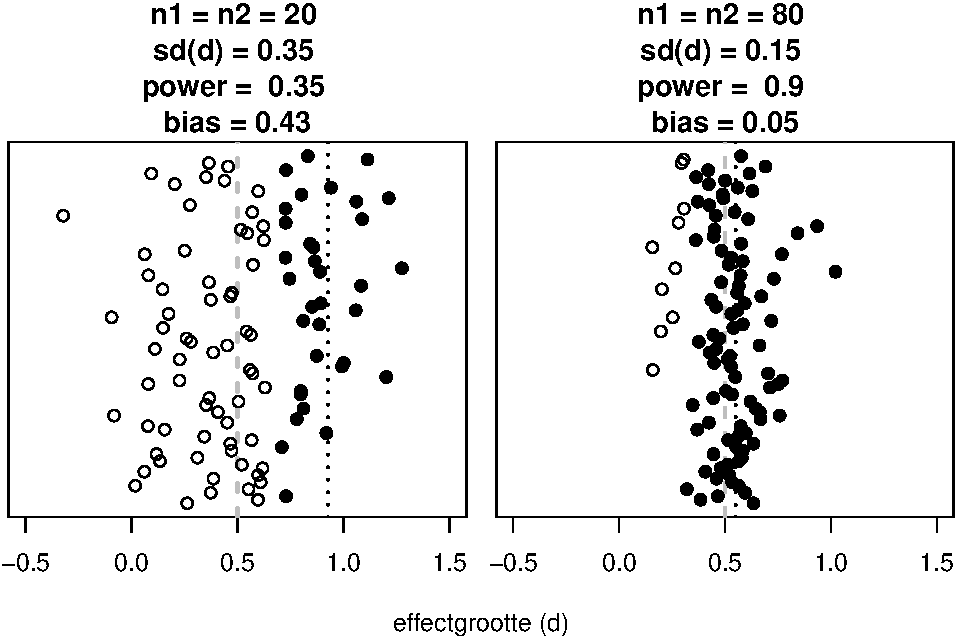
\includegraphics{KMS-NL_files/figure-latex/underpoweredeffectsizes-1.pdf}
De uitkomsten van gesimuleerde experimenten met verschillende
steekproefgrootte, en dus met verschillende power, zijn samengevat in
Figuur~\ref{fig:underpoweredeffectsizes}. We leggen het tweede nadeel uit aan de hand van deze wat complexe figuur. In het linker paneel van
Figuur~\ref{fig:underpoweredeffectsizes} zien we dat de verschillende
(simulaties van) `underpowered' onderzoeken een gemengd beeld laten
zien. Sommige van deze onderzoeken laten wèl een significant effect zien
(donkere symbolen), en veel andere onderzoeken niet (lichte symbolen).
Dat gemengde beeld leidt dan doorgaans tot vervolgonderzoek, waarin men
probeert om uit te zoeken \emph{waarom} het effect wel optrad in sommige
onderzoeken, en niet in andere. Zou het verschil in resultaten toe te
schrijven zijn aan verschillen in stimuli? proefpersonen? taken?
instrumentatie? Al dat vervolg-onderzoek is echter \emph{overbodig}: het
gemengde beeld van deze onderzoeken is goed te verklaren door de geringe
power van elk onderzoek. Het nodeloze en overbodige vervolg-onderzoek
kost veel tijd en geld (en indirecte kosten, zie
Hoofdstuk~\ref{ch:integriteit}), en het gaat ten koste van ander, nuttiger
onderzoek \citep[p.118]{Schm96}. Anders gezegd: één goed ontworpen studie met
ruim voldoende power kan vele nodeloze vervolg-studies voorkomen.

Het derde nadeel is gebaseerd op de ervaring dat onderzoek waarin wèl
een significant effect gevonden wordt (donkere symbolen), een grotere
kans heeft om gerapporteerd te worden; dit verschijnsel wordt
`publication bias' of het `file drawer problem' genoemd. Immers, een
positief resultaat wordt vaak wel gepubliceerd en een negatief resultaat
verdwijnt vaak in een bureaulade. Bij geringe power leidt dat tot een
derde nadeel, nl. een overschatting of `bias' van de gerapporteerde
effectgrootte. In een underpowered studie, immers, moet een gevonden
effect tamelijk groot zijn om gevonden te worden. In het meest linkse
paneel zien we dat er slechts \(31\times\) een significant effect gevonden
wordt. De gemiddelde effectgrootte van deze 31 significante uitkomsten
is \(\overline{d_{\textrm{signif}}}=0.90\) (zwarte stippellijn), d.w.z.
een vertekening of `bias' van \(0.40\) ten opzichte van de eigenlijke
\(d=0.50\) (grijze stippellijn)\footnote{Een replicatie-studie die wel voldoende power heeft, vindt dus typisch een kleiner effect dan de originele `underpowered' studie. Het kleinere effect gevonden in de replicatie-studie is dan typisch ook niet significant. We zeggen dan dat de replicatie-studie ``fails to replicate'' het effect dat in de originele studie wel significant was -- maar dat eigenlijk een spurieuze vondst was.}. In het meest rechtse paneel zien we dat
er \(91\times\) een significant effect gevonden wordt (dus de power is
hier voldoende). De gemiddelde effectgrootte van deze 91 significante
uitkomsten wijkt nauwelijks af van de eigenlijke \(d\). Bovendien is de
standaarddeviatie van de gerapporteerde effectgrootten kleiner, en dat
is weer van belang voor later onderzoek, meta-studies, en systematische
reviews.

Ten vierde brengt het gemengde beeld van de verschillende onderzoeken,
met soms wel en soms niet significante uitkomsten, en met grote variatie
in de gerapporteerde effectgrootte, het gevaar met zich mee dat deze
uitkomsten minder serieus genomen worden door `afnemers' van
wetenschappelijke kennis (behandelaars, zorgverzekeraars, ontwikkelaars,
beleidsmakers, e.d.). Deze afnemers krijgen zo de indruk dat de
wetenschappelijke evidentie voor dit onderzochte effect niet sterk is,
en/of dat de onderzoekers het oneens zijn over of dat effect bestaat en
zo ja hoe groot het dan is \citep{Kolf93} (Figuur~\ref{fig:underpoweredeffectsizes}).
Ook dat belemmert de
wetenschappelijke vooruitgang, en het belemmert het gebruik van
wetenschappelijke inzichten in maatschappelijke toepassingen.

Om al deze bezwaren te vermijden moeten onderzoekers al in een vroeg
stadium rekening houden met de gewenste power van een onderzoek. Het
opzetten en uitvoeren van een onderzoek met onvoldoende power is immers
in strijd met de eerder besproken ethische en morele principes van
zorgvuldigheid en verantwoordelijkheid
(§\ref{sec:integriteit-inleiding}).

\hypertarget{ch:variantieanalyse}{%
\chapter{Variantieanalyse}\label{ch:variantieanalyse}}

\hypertarget{sec:inleiding}{%
\section{Inleiding}\label{sec:inleiding}}

Dit hoofdstuk gaat over een veel gebruikte statistische analyse, genaamd
\emph{variantie-analyse} (Eng. `analysis of variance', vaak afgekort als
ANOVA). In dit hoofdstuk gebruiken we relatief veel Engelse
terminologie, ten eerste omdat de Nederlandse termen nauwelijks gebruikt
worden, en daarmee samenhangend om goed aan te sluiten bij de
Engelstalige vakliteratuur over variantieanalyse.

Hoe zit dit hoofdstuk in elkaar? We beginnen in
paragraaf~\ref{sec:anova-voorbeelden} met enkele voorbeelden van onderzoek
waarvan de uitkomsten getoetst kunnen worden met variantieanalyse. De
bedoeling van de paragraaf is je vertrouwd te maken met de techniek, met
de nieuwe terminologie, en met de voorwaarden waaronder van deze
techniek gebruik mag worden gemaakt. In
§\ref{sec:anova-oneway-uitleg} introduceren we de techniek op een
intuïtieve wijze door in te gaan op de gedachtegang achter de toets. In
§\ref{sec:anova-oneway-formeel} leiden we een formele vorm af voor
de belangrijkste toetsingsgrootheid, de \(F\)-ratio.

\hypertarget{sec:anova-voorbeelden}{%
\section{Enkele voorbeelden}\label{sec:anova-voorbeelden}}

Variantieanalyse is, net als de \emph{t}-toets, een statistische
generalisatietechniek, dat wil zeggen: een instrument dat gebruikt kan
worden bij de formulering van uitspraken over de eigenschappen van
populaties, op basis van gegevens ontleend aan steekproeven uit die
populaties. In het geval van de \emph{t}-toets en van ANOVA gaan die uitspraken over
het al dan niet gelijk zijn van de gemiddelden van (twee of meer)
populaties. In deze zin kan variantieanalyse dan ook opgevat worden als
een uitgebreide versie van de \emph{t}-toets: met ANOVA kunnen we gegevens analyseren
van meer dan twee steekproeven. Bovendien is het mogelijk om de effecten
van meerdere onafhankelijke variabelen simultaan in de analyse te
betrekken. Dat komt van pas als we gegevens willen analyseren uit een
factorieel ontwerp (§\ref{sec:ontwerp-factorieel}).

\begin{center}\rule{0.5\linewidth}{0.5pt}\end{center}

\begin{quote}
\emph{Voorbeeld 15.1}: In dit voorbeeld
onderzoeken we het spreektempo ofwel de spreeksnelheid van vier groepen
sprekers, nl. afkomstig uit het Midden, Noorden, Zuiden en Westen van
Nederland. De spreeksnelheid is uitgedrukt als de gemiddelde duur van
een lettergreep, gemiddeld over een interview van ca 15 minuten met elke
spreker \citep{Quene08} \citep{R-hqmisc}. Een kortere gemiddelde syllabeduur correspondeert
dus met een snellere spreker (vgl. de schaatssport: een kortere
rondetijd correspondeert met een snellere schaatser). Er waren 20
sprekers per groep, maar 1 spreker (uit het Zuiden) met een extreem hoge
waarde is hier verwijderd uit de steekproef.
\end{quote}

\begin{center}\rule{0.5\linewidth}{0.5pt}\end{center}

De geobserveerde spreeksnelheden per spreker uit bovenstaand voorbeeld 15.1
zijn samengevat in Tabel~\ref{tab:syldur} en
Figuur~\ref{fig:syldur-boxplot}. Hierbij is de regio van herkomst een
onafhankelijke categoriale variabele of `factor'. De waarden van deze
factor worden ook aangeduid als `nivo's' (Eng. `levels'), of in veel
onderzoeken als `groepen' of `condities'. Ieder nivo of iedere groep of
conditie vormt een `cel' van het ontwerp, en de observaties uit die cel
worden ook `replicaties' genoemd (bedenk waarom die zo genoemd worden).
De spreeksnelheid vormt de afhankelijke variabele. De nulhypothese luidt
dat de gemiddelden van de afhankelijke variabele gelijk zijn voor alle
groepen, dus H0: \(\mu_M = \mu_N = \mu_Z = \mu_W\). Als we H0 verwerpen,
dan betekent dat dus \emph{alleen} dat niet alle gemiddelden gelijk zijn,
maar het betekent \emph{niet} dat ieder groepsgemiddelde afwijkt van ieder
ander groepsgemiddelde. Daarvoor is nader (post-hoc) onderzoek nodig; we
komen daar later nog op terug.

\begin{longtable}[]{@{}lccc@{}}
\caption{\label{tab:syldur} Gemiddelde spreeksnelheden, met standaarddeviatie en aantallen sprekers, verdeeld naar regio van herkomst van de spreker (zie voorbeeld 15.1).}\tabularnewline
\toprule
regio & gemiddelde & s.d. & n\tabularnewline
\midrule
\endfirsthead
\toprule
regio & gemiddelde & s.d. & n\tabularnewline
\midrule
\endhead
Midden & 0.253 & 0.028 & 20\tabularnewline
Noord & 0.269 & 0.029 & 20\tabularnewline
Zuid & 0.260 & 0.030 & 19\tabularnewline
West & 0.235 & 0.028 & 20\tabularnewline
\bottomrule
\end{longtable}

\begin{figure}
\centering
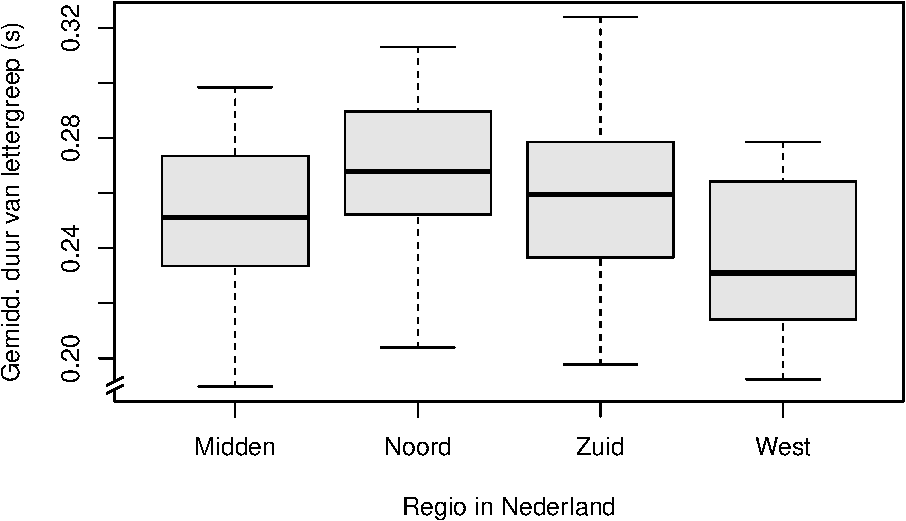
\includegraphics{KMS-NL_files/figure-latex/syldur-boxplot-1.pdf}
\caption{\label{fig:syldur-boxplot}Boxplot van de gemiddelde duur van de lettergrepen, opgesplitst naar regio van herkomst van de spreker.}
\end{figure}

Om nu te onderzoeken of de vier populaties verschillen in hun gemiddelde
spreeksnelheid, zouden we in eerste instantie en kunnen uitvoeren voor
alle paren van nivo's. (Met 4 nivo's zou dat 6 toetsen vereisen, zie
vergelijking \eqref{eq:choose} met \(n=4\) en \(x=2\)). Er kleven echter
verschillende bezwaren aan deze aanpak. Eén daarvan bespreken we hier.
Bij iedere gebruiken we een overschrijdingskans van \(\alpha=.05\). We
hebben dus een kans van .95 op een juiste beslissing zonder Type-I-fout.
De kans dat we bij alle 6 toetsen een juiste beslissing nemen is
\(.95^6 = .731\) (volgens de productregel,
vergelijking~\eqref{eq:kans-productregel}). De gezamenlijke kans op één of meer
Type-I-fout(en) in de 6 toetsen is dus niet meer \(.05\), maar is nu
opgelopen tot \(1-.731 = .265\), ruim een kwart!

Variantieanalyse nu biedt de mogelijkheid om op grond van één enkele
toetsing (dus niet 6 toetsen) de houdbaarheid te onderzoeken van de
bovengenoemde nulhypothese. Variantieanalyse kan dus het beste
gekenschetst worden als een globale toetsingstechniek, die het meest
geschikt is als je a priori geen specifieke voorspellingen kan of wil
doen omtrent de verschillen tussen de populaties.

Een variantieanalyse toegepast op de scores samengevat in
Tabel~\ref{tab:syldur}
zal tot verwerping van de nul-hypothese leiden: de 4 regionale
gemiddelden zijn niet gelijk. De gevonden verschillen zijn
hoogstwaarschijnlijk niet toe te schrijven aan toevallige
steekproeffluctuaties, maar aan systematische verschillen tussen de
groepen (\(\alpha=.05\)). Kan nu geconcludeerd worden dat de gevonden
verschillen in spreeksnelheid \emph{veroorzaakt} worden door verschil in
herkomst van de spreker? Hier is terughoudendheid geboden (zie
§\ref{sec:causaliteit}). Het is immers niet uit te sluiten dat de
vier populaties niet alleen in spreeksnelheid systematisch van elkaar
verschillen, maar ook in andere relevante factoren, die niet in het
onderzoek opgenomen zijn, zoals gezondheid, welvaart, of onderwijs. Die
andere factoren zouden we alleen kunnen uitsluiten als we proefpersonen
aselect zouden toewijzen aan de gekozen nivo's van de onafhankelijke
variabele. Dat is echter niet mogelijk als het gaat om de regio van
herkomst van de spreker: we kunnen een spreker meestal wel (aselect)
toewijzen aan een behandelvorm of conditie, maar niet aan een regio van
herkomst. In feite is het onderzoek in voorbeeld 15.1
dus quasi-experimenteel.

Voor ons tweede voorbeeld betrekken we een tweede factor in hetzelfde
onderzoek naar spreeksnelheid, nl. ook het geslacht van de spreker.
ANOVA stelt ons in staat om in één enkele analyse te toetsen of (i) de vier
regio's van elkaar verschillen (H0: \(\mu_M = \mu_N = \mu_Z = \mu_W\)), en
of (ii) de twee geslachten van elkaar verschillen (H0:
\(\mu_\textrm{vrouw} = \mu_\textrm{man}\)), en of (iii) de verschillen
tussen de regio's hetzelfde zijn voor beide geslachten (of, anders
gezegd, of de verschillen tussen de geslachten hetzelfde zijn voor alle
regio's). Dat laatste noemen we de `interactie' tussen de twee factoren.

\begin{longtable}[]{@{}llccc@{}}
\caption{\label{tab:syldur2way} Gemiddelde spreeksnelheden, met standaarddeviatie en aantallen sprekers, verdeeld naar geslacht en regio van herkomst van de spreker (zie voorbeeld 15.1).}\tabularnewline
\toprule
geslacht & regio & gemiddelde & s.d. & n\tabularnewline
\midrule
\endfirsthead
\toprule
geslacht & regio & gemiddelde & s.d. & n\tabularnewline
\midrule
\endhead
vrouw & Midden & 0.271 & 0.021 & 10\tabularnewline
vrouw & Noord & 0.285 & 0.025 & 10\tabularnewline
vrouw & Zuid & 0.269 & 0.028 & 9\tabularnewline
vrouw & West & 0.238 & 0.028 & 10\tabularnewline
man & Midden & 0.235 & 0.022 & 10\tabularnewline
man & Noord & 0.253 & 0.025 & 10\tabularnewline
man & Zuid & 0.252 & 0.030 & 10\tabularnewline
man & West & 0.232 & 0.028 & 10\tabularnewline
\bottomrule
\end{longtable}

De resultaten in Tabel~\ref{tab:syldur2way} suggereren dat (i) sprekers uit het Westen
sneller spreken dan de anderen, en dat (ii) mannen sneller spreken dan
vrouwen (!). En (iii) het verschil tussen mannen en vrouwen lijkt
kleiner voor sprekers uit het Westen dan voor sprekers uit andere
regionen.

\hypertarget{aannames-2}{%
\subsection{aannames}\label{aannames-2}}

De variantie-analyse vereist vier aannames (of assumpties) waaraan
voldaan moet zijn, om deze toets te mogen gebruiken; deze aannames komen
overeen met die van de \emph{t}-toets
(§\ref{sec:ttoets-aannames}).

\begin{itemize}
\item
  De gegevens moeten gemeten zijn op intervalniveau (zie
  §\ref{sec:interval}).
\item
  Alle observaties moeten onafhankelijk van elkaar zijn.
\item
  De scores moeten normaal verdeeld zijn (zie
  §\ref{sec:isvarnormaalverdeeld}).
\item
  De variantie van de scores moet (ongeveer) gelijk zijn in de
  scores van de respectievelijke groepen of condities (zie
  §\ref{sec:variantie}).
  Schending van deze aanname is ernstiger
  naarmate de steekproeven meer in grootte verschillen. Het is daarom
  verstandig om te werken met even grote, en liefst niet te kleine
  steekproeven.
\end{itemize}

Samenvattend: variantieanalyse kan gebruikt worden om meerdere
populatiegemiddelden te vergelijken, en om de effecten van meerdere
factoren en combinaties van factoren (interacties) te bepalen.
Variantieanalyse vereist wel dat de gegevens aan meerdere voorwaarden
voldoen.

\hypertarget{euxe9n-weg-variantieanalyse}{%
\section{Eén-weg-variantieanalyse}\label{euxe9n-weg-variantieanalyse}}

\hypertarget{sec:anova-oneway-uitleg}{%
\subsection{Een intuïtieve uitleg}\label{sec:anova-oneway-uitleg}}

Zoals gezegd gebruiken we variantieanalyse om te onderzoeken of de
scores van verschillende groepen, of verzameld onder verschillende
condities, van elkaar verschillen. Maar --- scores verschillen \emph{altijd}
van elkaar, door toevallige fluctuaties tussen de replicaties binnen
elke steekproef. In de voorgaande hoofdstukken zijn we al vele
voorbeelden tegengekomen van toevalsfluctuaties binnen dezelfde
steekproef en binnen dezelfde conditie. De vraag wordt dan, of de scores
\emph{tussen} de verschillende groepen (of verzameld onder verschillende
condities) méér van elkaar verschillen dan je zou verwachten op grond
van toevallige fluctuaties \emph{binnen} elke groep of cel.

De bovengenoemde ``verschillen tussen scores'' vormen bij elkaar de
variantie van die scores
(§\ref{sec:variantie}). Bij variantieanalyse verdelen we de totale
variantie in twee delen: ten eerste de variantie veroorzaakt door
(systematische) verschillen \emph{tussen} groepen, en ten tweede de variantie
veroorzaakt door (toevallige) verschillen \emph{binnen} groepen. Als H0 waar
is, en als er dus (in de populaties) géén verschillen tussen de groepen
zijn, dan verwachten we desalniettemin (in de steekproeven van de
groepen) wèl enige verschillen tussen de gemiddelde scores van de
groepen, zij het dat de laatstgenoemde verschillen niet groter zullen
zijn dan de toevallige verschillen binnen de groepen, als H0 waar is.
Lees deze alinea nog eens aandachtig door.

Deze aanpak wordt geïllustreerd in
Figuur~\ref{fig:kleurtjes-obs}, waarin de scores zijn afgebeeld uit drie
experimentele groepen (met aselecte toewijzing van proefpersonen aan de
groepen): de rode, grijze en blauwe groep. De scores verschillen van
elkaar, in ieder geval door toevallige fluctuaties van de scores binnen
elke groep. Er zijn misschien ook systematische verschillen tussen (de
gemiddelde scores van) de drie groepen. Maar zijn deze systematische
verschillen nu relatief groter dan de toevallige verschillen binnen
groepen? Zo ja, dan verwerpen we H0.

\begin{figure}
\centering
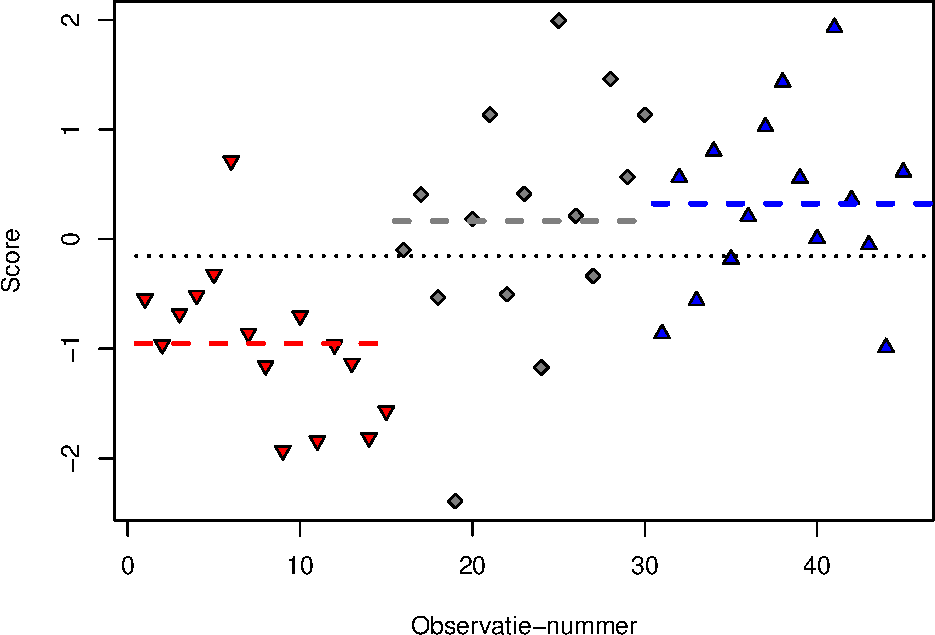
\includegraphics{KMS-NL_files/figure-latex/kleurtjes-obs-1.pdf}
\caption{\label{fig:kleurtjes-obs}Gesimuleerde observaties van drie experimentele groepen: rood (neerwaartse driehoek), grijs (ruit), en blauw (opwaartse driehoek) (n=15 per groep), met het gemiddelde per groep (in streeplijnen), en met het gemiddelde over alle observaties (stippellijn).}
\end{figure}

De systematische verschillen \emph{tussen} de groepen corresponderen met de
verschillen van de rode, grijze en blauwe groepsgemiddelden
(streepjeslijnen in
Figuur~\ref{fig:kleurtjes-obs}) ten opzichte van het gemiddelde over
alle observaties (stippellijn). Voor de eerste observatie is dat een
negatieve afwijking, want de score ligt onder het algemene gemiddelde
(stippellijn). De toevallige verschillen \emph{binnen} de groepen
corresponderen met de afwijking van iedere observatie ten opzichte van
het groepsgemiddelde (voor de eerste observatie is dat dus een positieve
afwijking, want de score ligt boven het groepsgemiddelde van de rode
groep).

Laten we nu de overstap maken van `verschillen' naar `variantie'. We
splitsen dan de afwijking van iedere observatie t.o.v. het algemene
gemiddelde op in twee afwijkingen: ten eerste de afwijking van
groepsgemiddelde t.o.v. algemene gemiddelde, en ten tweede de afwijking
van iedere replicatie t.o.v. het groepsgemiddelde. Dat zijn twee stukjes
variantie, die tezamen de totale variantie vormen. Omgekeerd kunnen we
dus de totale variantie opdelen in deze twee componenten, vandaar de
naam `variantieanalyse'. (We zullen in de volgende paragraaf uitleggen
hoe die componenten berekend worden, rekening houdend met het aantal
observaties en aantal groepen.)

Die verdeling van de totale variantie in twee variantiecomponenten is
nuttig, omdat we daarna de \emph{verhouding} of ratio tussen die twee delen
kunnen bepalen. Die verhouding tussen varianties wordt de \(F\)-ratio
genoemd, en we gebruiken deze verhouding om H0 te toetsen.

\[\textrm{H0}: \textrm{variantie tussen groepen} = \textrm{variantie binnen groepen}\]

\[\textrm{H0}: F = \frac{\textrm{variantie tussen groepen}}{\textrm{variantie binnen groepen}} = 1\]

De \(F\)-ratio is dus een toetsingsgrootheid, waarvan de kansverdeling
bekend is indien H0 waar is. In het voorbeeld van
Figuur~\ref{fig:kleurtjes-obs} vinden we \(F=3.22\), met 3 groepen en 45
observaties, \(p=.0004\). We vinden hier dus een relatief grote
systematische variantie \emph{tussen} groepen, ten opzichte van de relatief
kleine toevallige variantie \emph{binnen} groepen: de eerstgenoemde variantie
(teller van verhouding \(F\)) is meer dan \(3\times\) zo groot als de
laatstgenoemde variantie (noemer van verhouding \(F\)). De kans \(p\) om
deze verhouding te vinden als H0 waar is, is buitengewoon gering, en we
verwerpen daarom H0. (We zullen in de volgende paragraaf uitleggen hoe
die kans bepaald wordt, weer rekening houdend met het aantal observaties
en aantal groepen.) We spreken dan van een significant effect van de
factor op de afhankelijke variabele.

Aan het slot van deze paragraaf herhalen we de essentie van de
variantieanalyse. We verdelen de totale variantie in twee delen: de
mogelijk systematische variantie tussen groepen of condities, en de
variantie binnen groepen of condities (d.i. altijd aanwezige, toevallige
fluctuatie tussen replicaties). De toetsingsgrootheid \(F\) bestaat uit de
verhouding tussen deze twee varianties. We toetsen eenzijdig of \(F=1\),
en verwerpen H0 als \(F>1\) zodanig dat de kans
\(P(F|\textrm{H0}) < \alpha\). De gemiddelde scores van de groepen of
condities zijn dan hoogstwaarschijnlijk niet alle gelijk. We weten
daarmee nog niet welke groepen van elkaar verschillen, daarvoor is nog
verdere (post-hoc) analyse nodig
(§\ref{sec:anova-oneway-posthoc} hieronder).

\hypertarget{sec:anova-oneway-formeel}{%
\subsection{Een formele uitleg}\label{sec:anova-oneway-formeel}}

Voor onze uitleg beginnen we met de geobserveerde scores. We nemen aan
dat de scores zijn opgebouwd volgens een bepaald statistisch model, nl.
als de optelsom van het populatiegemiddelde (\(\mu\)), een systematisch
effect (\(\alpha_j\)) van de \(j\)'de conditie of groep (over \(k\) condities
of groepen), en een toevallig effect (\(e_{ij}\)) voor de \(i\)'de
replicatie binnen de \(j\)'de conditie of groep (over \(N\) replicaties in
totaal). In formule:
\[x_{ij} = \mu + \alpha_{j} + e_{ij}\]
Ook hier
weer ontleden we dus iedere score in een systematisch deel en een
toevallig deel. Dat geldt niet alleen voor de scores zelf, maar ook voor
de afwijkingen van iedere score ten opzichte van het totale gemiddelde
(zie §\ref{sec:anova-oneway-uitleg}).

Er zijn derhalve drie varianties van belang. Ten eerste de totale
variantie (zie vergelijking
\eqref{eq:variantie}, afgekort tot \texttt{t}) over alle \(N\)
observaties uit alle groepen of condities tezamen:
\begin{equation}
  \label{eq:MStotal}
    s^2_t = \frac{ \sum (x_{ij} - \overline{x})^2 } {N-1}
\end{equation}
Ten tweede de variantie tussen (Eng. `between', afgekort tot\texttt{b}) de
groepen of condities:
\begin{equation}
  \label{eq:MSbetween}
    s^2_b = \frac{ \sum_{j=1}^{j=k} n_j (\overline{x_j} - \overline{x})^2 } {k-1}
\end{equation}
en ten derde de variantie binnen (Eng. `within', afgekort tot \texttt{w}) de
groepen of condities:
\begin{equation}
  \label{eq:MSwithin}
    s^2_w = \frac{ \sum_{j=1}^{j=k} \sum_i (x_{ij} - \overline{x_j})^2 } {N-k}
\end{equation}

In deze vergelijkingen worden de \emph{tellers} gevormd door de som van de
gekwadrateerde afwijkingen (`sums of squares', afgekort \texttt{SS}). In de
vorige paragraaf hebben we aangegeven dat de afwijkingen bij elkaar
optellen, en dat geldt dan ook voor de gesommeerde en gekwadrateerde
afwijkingen:
\begin{align}
  \label{eq:SStotal}
    { \sum (x_{ij} - \overline{x})^2 } &= 
    { \sum_{j=1}^{j=k} n_j (\overline{x_j} - \overline{x})^2 } + 
    { \sum_{j=1}^{j=k} \sum_i (x_{ij} - \overline{x_j})^2 } \\
    \textrm{SS}_t &= \textrm{SS}_b + \textrm{SS}_w
\end{align}
De
\emph{noemers} van de varianties worden gevormd door de vrijheidsgraden
(`degrees of freedom', afgekort \texttt{df}, zie
§\ref{sec:ttoets-vrijheidsgraden}). Voor de variantie tussen
groepen \(s^2_b\) is dat het aantal groepen of condities, minus 1 (\(k-1\)).
Voor de variantie binnen groepen \(s^2_w\) is dat het aantal observaties,
minus het aantal groepen (\(N-k\)). Voor de totale variantie is dat het
aantal observaties minus 1 (\(N-1\)). Ook de vrijheidsgraden van de
afwijkingen tellen bij elkaar op:
\begin{align}
  \label{eq:dftotal1}
    { (N-1) } &= { (k-1) } + { (N-k) } \\
    \textrm{df}_t &= \textrm{df}_b + \textrm{df}_w
\end{align}

De bovenstaande breuken die de varianties \(s^2_t\), \(s^2_b\) en \(s^2_w\)
beschrijven, worden ook aangeduid als de `mean squares' (afgekort \texttt{MS}).
\(\textrm{MS}_{t}\) is per definitie gelijk aan de `gewone' variantie
\(s^2_x\) (zie de identieke vergelijkingen
\eqref{eq:variantie} en
\eqref{eq:MStotal}).

De toetsingsgrootheid \(F\) is gedefinieerd als de verhouding van de twee
hierboven gedefinieerde variantiecomponenten:
\begin{equation}
  \label{eq:Fratio}
    F = \frac{ s^2_b } { s^2_w }
\end{equation}
met niet één maar twee
vrijheidsgraden, resp. \((k-1)\) voor de teller en \((N-k)\) voor de noemer.

De overschrijdingskans \(p\) die behoort bij de gevonden \(F\) kan je
bepalen aan de hand van een tabel, maar meestal voeren we een
variantieanalyse uit met behulp van de computer, en die berekent dan ook
die overschrijdingskans.

De resultaten van een variantieanalyse worden samengevat met een vaste
opbouw in een zgn. ANOVA-tabel, zoals
Tabel~\ref{tab:kleurtjes-anova}. Daarin staat de belangrijkste
informatie samengevat. Maar de hele tabel kan ook in één zin samengevat
worden, zie Voorbeeld 15.2

\begin{longtable}[]{@{}lrcccc@{}}
\caption{\label{tab:kleurtjes-anova} Samenvatting van variantieanalyse van de observaties in Figuur~\ref{fig:kleurtjes-obs}.}\tabularnewline
\toprule
variantiebron & df & SS & MS & \(F\) & \(p\)\tabularnewline
\midrule
\endfirsthead
\toprule
variantiebron & df & SS & MS & \(F\) & \(p\)\tabularnewline
\midrule
\endhead
groep & 2 & 14.50 & 7.248 & 9.356 & 0.0004\tabularnewline
(within) & 42 & 32.54 & 0.775 & &\tabularnewline
\bottomrule
\end{longtable}

\begin{center}\rule{0.5\linewidth}{0.5pt}\end{center}

\begin{quote}
\emph{Voorbeeld 15.2}:
De gemiddelde scores zijn niet gelijk voor de rode, grijze en blauwe groep
{[}\(F(2,42) = 9.35, p = .0004, \omega^2 = 0.28\){]}.
\end{quote}

\begin{center}\rule{0.5\linewidth}{0.5pt}\end{center}

\hypertarget{sec:anova-oneway-effectgrootte}{%
\subsection{Effectgrootte}\label{sec:anova-oneway-effectgrootte}}

Net als bij de \(t\)-toets is het niet alleen van belang om een binaire beslissing
te nemen over H0, maar is het minstens zo belangrijk om te weten hoe
groot het geobserveerde effect is (zie ook
§\ref{sec:ttoets-effectgrootte}). Deze effectgrootte bij
variantieanalyse kan worden uitgedrukt in verschillende maten, waarvan
wij er twee bespreken (deze paragraaf is gebaseerd op \citet{KL00}; zie ook \citet{Olej03}).

De eenvoudigste maat is de zgn. \(\eta^2\) (``èta-kwadraat'' of ``eta
squared''), de proportie van de totale SS die toe te schrijven is aan de
verschillen tussen de groepen of condities: \[\label{eq:etasq}
    \eta^2 = \frac{ \textrm{SS}_b } { \textrm{SS}_t }\] De effectgrootte
\(\eta^2\) is een proportie tussen 0 en 1, die aangeeft hoeveel van de
variantie in de \emph{steekproef} toe te schrijven is aan de onafhankelijke
variabele.

De tweede maat voor effectgrootte bij variantieanalyse is de zgn.
\(\omega^2\) (``omega-kwadraat'' of ``omega squared''):
\begin{equation}
  \label{eq:omegasq}
    \omega^2 = \frac{ \textrm{SS}_b - (k-1) \textrm{MS}_w} { \textrm{SS}_t + \textrm{MS}_w }
\end{equation}
De effectgrootte \(\omega^2\) is ook een proportie; dit is een schatting
van de proportie van de variantie in de \emph{populatie} die toe te schrijven
is aan de onafhankelijke variabele, waarbij de schatting uiteraard
gebaseerd is op de onderzochte steekproef. Omdat we in het algemeen meer
geïnteresseerd zijn in generalisatie naar de populatie dan naar de
steekproef, geven wij de voorkeur aan \(\omega^2\) als maat voor de
effectgrootte.

We dienen niet alleen de \(F\)-ratio, vrijheidsgraden, en
overschrijdingskans te rapporteren, maar ook de effectgrootte (zie
voorbeeld 15.2 hierboven).

\begin{quote}
``It is not enough to report
\(F\)-ratios and whether they are statistically significant. We must know
how strong relations are. After all, with large enough \(N\)s, \(F\)- and
\(t\)-ratios can almost always be statistically significant. While often
sobering in their effect, especially when they are low, coefficients of
association of independent and dependent variables {[}i.e., effect size
coefficients{]} are \emph{indispensable} parts of research results'' \citep[ p.327, nadruk toegevoegd]{KL00}.
\end{quote}

\hypertarget{sec:anova-oneway-gericht}{%
\subsection{Gerichte vergelijkingen}\label{sec:anova-oneway-gericht}}

In voorbeeld 15.2 (zie
Figuur~\ref{fig:kleurtjes-obs}) onderzochten we de verschillen tussen
scores uit de rode, zwarte en blauwe groepen. De nulhypothese die
getoetst werd was H0:
\(\mu_\textrm{rood} = \mu_\textrm{grijs} = \mu_\textrm{blauw}\).
Het is
echter ook goed mogelijk dat een onderzoeker al bepaalde ideeën heeft
over de verschillen tussen de groepen, en \emph{gericht} op zoek is naar
bepaalde verschillen, en andere verschillen juist wil negeren. De
gerichte vergelijkingen (Eng. `planned comparisons') worden ook wel
`contrasten' genoemd.

Laten we voor hetzelfde voorbeeld aannemen dat de onderzoeker al
verwacht, uit eerder onderzoek, dat de scores van de rode en blauwe
groepen van elkaar zullen verschillen. De bovenstaande H0 is dan niet
meer interessant om te onderzoeken, omdat we bij voorbaat verwachten H0
te zullen verwerpen. De onderzoeker wil nu gericht weten
(1) of de rode
groep lager scoort dan de andere twee groepen, (H0:
\(\mu_\textrm{rood} = (\mu_\textrm{grijs}+\mu_\textrm{blauw})/2\)), en
(2)
of de grijze en blauwe groepen van elkaar verschillen (H0:
\(\mu_\textrm{grijs} = \mu_\textrm{blauw}\))
\footnote{Als (1) rood wel verschilt van grijs en blauw, en als (2) grijs en blauw bovendien onderling niet verschillen, dan impliceert dat dat rood verschilt van grijs (een nieuwe bevinding) en dat rood verschilt van blauw (dat wisten we al).}.

De factor `groep' of `kleur' heeft 2 vrijheidsgraden, en dat betekent dat we
precies 2 van zulke gerichte vergelijkingen of `contrasten' kunnen maken
die onafhankelijk zijn van elkaar. Dergelijke onafhankelijke contrasten
worden `orthogonaal' genoemd.

In een variantieanalyse met gerichte vergelijkingen wordt de variantie
tussen groepen of condities nog verder opgedeeld, nl. in de gerichte
contrasten zoals de twee hierboven (zie
Tabel~\ref{tab:kleurtjes-anova-contrast}). We laten een verdere uitleg
over gerichte vergelijkingen hier achterwege, maar adviseren wel om waar
mogelijk slim gebruik te maken van deze gerichte vergelijkingen, indien
je een meer specifieke nulhypothese kunt opstellen dan H0: ``de
gemiddelde scores zijn gelijk in alle groepen of condities''. We kunnen
zo gerichte uitspraken doen over de verschillen tussen de groepen in ons
voorbeeld:

\begin{center}\rule{0.5\linewidth}{0.5pt}\end{center}

\begin{quote}
\emph{Voorbeeld 15.3}:
De gemiddelde score van de rode
groep is significant lager dan van de beide andere groepen gecombineerd
{[}\(F(1,42)=18.47, p=.0001, \omega^2=0.28\){]}. De gemiddelde score is
nagenoeg gelijk voor de grijze en blauwe groep
{[}\(F(1,42)<1, \textrm{n.s.}, \omega^2=0.00\){]}.
Dit impliceert dat de
rode groep significant lagere scores behaalt dan de grijze groep en dan
de blauwe groep.
\end{quote}

\begin{center}\rule{0.5\linewidth}{0.5pt}\end{center}

\begin{longtable}[]{@{}lrcccc@{}}
\caption{\label{tab:kleurtjes-anova-contrast} Samenvatting van variantieanalyse van de observaties in Figuur~\ref{fig:kleurtjes-obs}, met gerichte contrasten tussen groepen.}\tabularnewline
\toprule
variantiebron & df & SS & MS & \(F\) & \(p\)\tabularnewline
\midrule
\endfirsthead
\toprule
variantiebron & df & SS & MS & \(F\) & \(p\)\tabularnewline
\midrule
\endhead
groep & 2 & 14.50 & 7.248 & 9.356 & 0.0004\tabularnewline
~~groep, contrast 1 & 1 & 14.31 & 14.308 & 18.470 & 0.0001\tabularnewline
~~groep, contrast 2 & 1 & 0.19 & 0.188 & 0.243 & 0.6248\tabularnewline
(within) & 42 & 32.54 & 0.775 & &\tabularnewline
\bottomrule
\end{longtable}

De variantie-analyse met gerichte vergelijkingen is dus vooral bruikbaar
als je, voordat de observaties zijn gedaan, al gerichte hypotheses hebt
over verschillen tussen bepaalde (combinaties van) groepen of condities.
Die hypotheses kunnen gebaseerd zijn op theoretische overwegingen, of op
eerdere onderzoeksresultaten.

\hypertarget{orthogonale-contrasten}{%
\subsubsection{Orthogonale contrasten}\label{orthogonale-contrasten}}

Elk contrast kan worden uitgedrukt in de vorm van gewichten voor iedere
conditie. Voor de hierboven besproken contrasten kan dat in de vorm van
deze gewichten:

\begin{longtable}[]{@{}ccc@{}}
\toprule
conditie & contrast 1 & contrast 2\tabularnewline
\midrule
\endhead
~~rood & -1 & 0\tabularnewline
~~grijs & +0.5 & -1\tabularnewline
~~blauw & +0.5 & +1\tabularnewline
\bottomrule
\end{longtable}

De H0 voor contrast 2 (\(\mu_\textrm{grijs} = \mu_\textrm{blauw}\)) is uit
te drukken in gewichten als volgt:
\(\textrm{C2} = 0\times \mu_\textrm{rood} -1 \times \mu_\textrm{grijs} +1 \times \mu_\textrm{blauw} = 0\).

Om te bepalen of twee contrasten orthogonaal zijn, vermenigvuldigen we
hun respectievelijke gewichten voor iedere conditie (rij):\\
\(( (-1)(0), (+0.5)(-1), (+0.5)(+1) )= (0, -0.5, +0.5)\).\\
Vervolgens tellen we al deze producten bij elkaar op:
\(0 -0.5 + 0.5 = 0\). Als de som van deze producten nul is, dan zijn de
twee contrasten orthogonaal.

\hypertarget{sec:anova-oneway-posthoc}{%
\subsection{Post-hoc vergelijkingen}\label{sec:anova-oneway-posthoc}}

In veel onderzoeken heeft een onderzoeker géén idee over de te
verwachten verschillen tussen de groepen of condities. Pas na afloop van
de variantieanalyse, \emph{nadat} er een significant effect gevonden is,
besluit de onderzoeker om nader te inspecteren welke condities van
elkaar verschillen. We spreken dan van \emph{post-hoc} vergelijkingen,
``suggested by the data'' \citep[ p.200]{MD04}. We moeten daarbij conservatief te
werk gaan, juist omdat we na de variantieanalyse al kunnen vermoeden dat
sommige vergelijkingen een significant resultaat zullen opleveren,
d.w.z., de nulhypotheses zijn al niet neutraal.

Er zijn vele tientallen statistische toetsen voor post-hoc
vergelijkingen. Het belangrijkste verschil is hun mate van conservatisme
(neiging om H0 niet te verwerpen) vs.~liberalisme (neiging om H0 wel te
verwerpen). Daarnaast zijn sommige toetsen meer ingericht op
paarsgewijze vergelijkingen tussen condities (`pairwise comparisons',
zoals contrast 2 hierboven) en andere meer op complexe vergelijkingen
(zoals contrast 1 hierboven). En de toetsen verschillen in de aannames
die ze doen over de varianties in de cellen. We noemen hier één toets
voor post-hoc-vergelijkingen tussen paren van condities: \emph{Tukey's
Honestly Significant Difference}, afgekort Tukey's HSD. Deze toets neemt
een goede middenpositie in tussen te conservatief of te liberaal. Een
belangrijke eigenschap van de Tukey HSD toets is dat de \emph{gezamenlijke}
overschrijdingskans (Eng. `family-wise error') over alle paarsgewijze
vergelijkingen tezamen gelijk is aan de opgegeven overschrijdingskans
\(\alpha\) (zie §\ref{sec:anova-voorbeelden}). De Tukey HSD toets resulteert in
een 95\% betrouwbaarheidsinterval van het verschil tussen twee condities,
en/of in een \(p\)-waarde van het verschil tussen twee condities.

\hypertarget{spss-12}{%
\subsection{SPSS}\label{spss-12}}

\hypertarget{voorbereiding}{%
\subsubsection{voorbereiding}\label{voorbereiding}}

We gebruiken de gegevens in het bestand \texttt{data/kleurgroepen.txt}; deze gegevens zijn ook weergegeven in Figuur \ref{fig:kleurtjes-obs}.
Lees eerst de benodigde gegevens, en controleer deze:

\begin{verbatim}
File > Import Data > Text Data...
\end{verbatim}

Selecteer \texttt{Files\ of\ type:\ Text} en selecteer bestand
\texttt{data/kleurgroepen.txt}. Bevestig met \texttt{Open}.\\
Namen van variabelen staan op regel 1. Decimale symbool is punt
(period). Data beginnen op regel 2. Elke regel is een observatie. De
gebruikte scheiding (delimiter) tussen variabelen is een spatie. Tekst
staat tussen dubbele aanhalingstekens. De variabelen hoef je niet verder
te definiëren, de standaardopties van SPSS werken hier goed.\\
Bevestig het laatste keuzescherm met \texttt{Done}. De gegevens
worden dan ingelezen.

Onderzoek of de responsies normaal verdeeld zijn, met behulp van de
technieken uit Deel II van dit tekstboek (met name
§\ref{sec:isvarnormaalverdeeld}).

We kunnen in SPSS niet vooraf toetsen of de varianties gelijk zijn in de
drie groepen, zoals vereist voor variantieanalyse. We doen dat tegelijk
met de variantieanalyse zelf.

\hypertarget{anova}{%
\subsubsection{ANOVA}\label{anova}}

In SPSS kan je een variantieanalyse op meerdere manieren uitvoeren. We
gebruiken hier een algemeen bruikbare aanpak, waarbij we aangeven dat er
één afhankelijke variabele in het spel is.\\

\begin{verbatim}
Analyze > General Linear Model > Univariate...
\end{verbatim}

Selecteer \texttt{score} als afhankelijke variabele (sleep naar paneel
``Dependent variable'').\\
Selecteer \texttt{kleur} als onafhankelijke variabele (sleep naar paneel ``Fixed
Factor(s)'').\\
Kies \texttt{Model...} en daarna \texttt{Full\ factorial} model, \texttt{Type\ I} Sum
of squares, en vink aan: \texttt{Include\ intercept\ in\ model}, en bevestig met
\texttt{Continue}.\\
Kies \texttt{Options...} en vraag om gemiddelden voor de condities
van de factor \texttt{kleur} (sleep naar paneel ``Display Means for''). Vink aan:
\texttt{Estimates\ of\ effect\ size} en \texttt{Homogeneity\ tests}, en bevestig weer met
\texttt{Continue}.\\
Bevestig alle keuzes met \texttt{OK}.

In de uitvoer vinden we eerst de uitslag van Levene's toets op gelijke
varianties (homogeniteit van variantie), die geen aanleiding geeft om H0
te verwerpen. We mogen dus een variantieanalyse uitvoeren.

Daarna wordt de variantieanalyse samengevat in een tabel gelijkend op
Tabel~\ref{tab:kleurtjes-anova}, waarbij ook de effectgrootte vermeld
wordt in de vorm van \texttt{~Partial\ eta\ square}. Het is echter beter om
\(\omega^2\) te rapporteren, maar je moet die dan wel zelf uitrekenen!

\hypertarget{gerichte-vergelijking}{%
\subsubsection{gerichte vergelijking}\label{gerichte-vergelijking}}

Voor een variantieanalyse met gerichte vergelijkingen moeten we de
gewenste contrasten aangeven voor de factor \texttt{kleur}. De werkwijze is
echter anders dan hierboven. We kunnen de gerichte contrasten in SPSS
niet opgeven via het menu-systeem dat we tot nu toe gebruikten. We
moeten hiervoor ``onder de motorkap'' gaan werken!\\
Herhaal daartoe eerst de instructies hierboven. Maar, in plaats van
alles te bevestigen, kies je nu de knop \texttt{Paste}. Er wordt dan
een zgn. Syntax-venster geopend (of geactiveerd, als het al open was).
Je ziet daarin het SPSS-commando dat je via het menu hebt opgebouwd. We
gaan dit commando bewerken om onze eigen, speciale contrasten aan te
geven. Bij het specificeren van de contrasten moeten we wel rekening
houden met de \emph{alfabetische} ordening van de condities: blauw, grijs,
rood.\\
Het commando in het Syntax-venster moet er uiteindelijk uitzien als
hieronder, nadat je de regel \texttt{/CONTRAST} hebt toegevoegd. Het commando
moet worden afgesloten met een punt.\\

\begin{verbatim}
UNIANOVA score BY kleur
  /METHOD=SSTYPE(1)
  /INTERCEPT=INCLUDE
  /EMMEANS=TABLES(kleur) 
  /PRINT=ETASQ HOMOGENEITY
  /CRITERIA=ALPHA(.05)
  /DESIGN=kleur
  /CONTRAST(kleur)=special(0.5 0.5 -1, 1 -1 0).
\end{verbatim}

Plaats de cursor ergens tussen het woord \texttt{UNIANOVA} en de afsluitende
punt, en klik dan op de grote groene pijl naar rechts (\texttt{Run\ Selection})
in het menu van het Syntax-venster.

De uitvoer geeft voor ieder contrast de significantie en het
betrouwbaarheidsinterval van het getoetste contrast. Het eerste contrast
is wel significant (\texttt{Sig.\ .000}, rapporteer als \(p<.001\), zie §\ref{sec:pgroterdannul}), en het tweede niet, zie
Tabel~\ref{tab:kleurtjes-anova-contrast}.

\hypertarget{post-hoc-vergelijking}{%
\subsubsection{post-hoc-vergelijking}\label{post-hoc-vergelijking}}

Herhaal eerst de instructies hierboven.\\
Kies de knop \texttt{Post\ Hoc...}, en selecteer de factor \texttt{kleur}
(verplaats naar venster ``Post Hoc Tests for:''). Vink aan: \texttt{Tukey}, en
daarna \texttt{Continue}. Bevestig alle keuzes met \texttt{OK}.

Voor iedere paarsgewijze vergelijking zien we het verschil, de
standaardfout, en de ondergrens (\texttt{Lower\ Bound}) en bovengrens
(\texttt{Upper\ Bound}) van het 95\% betrouwbaarheidsinterval van dat verschil.
Als dat interval \emph{niet} nul omvat, dan is het verschil tussen de twee
groepen of condities dus waarschijnlijk niet gelijk aan nul. De
gecorrigeerde overschrijdingskans volgens Tukey's HSD toets is bovendien
gegeven in de derde kolom. We zien dat rood verschilt van blauw, dat
rood verschilt van grijs, en dat de scores van de grijze en blauwe
groepen niet verschillen.

\hypertarget{r-14}{%
\subsection{R}\label{r-14}}

\hypertarget{voorbereiding-1}{%
\subsubsection{voorbereiding}\label{voorbereiding-1}}

Lees eerst de benodigde gegevens, en controleer deze:

\begin{Shaded}
\begin{Highlighting}[]
\CommentTok{\# zelfde data als gebruikt in Fig.15.2}
\NormalTok{kleurgroepen \textless{}{-}}\StringTok{ }\KeywordTok{read.table}\NormalTok{( }\StringTok{"data/kleurgroepen.txt"}\NormalTok{, }
                            \DataTypeTok{header=}\OtherTok{TRUE}\NormalTok{, }\DataTypeTok{stringsAsFactors=}\OtherTok{TRUE}\NormalTok{ )}
\end{Highlighting}
\end{Shaded}

Onderzoek of de responsies normaal verdeeld zijn, met behulp van de
technieken uit Deel II van dit tekstboek (met name
§\ref{sec:isvarnormaalverdeeld}).

Onderzoek of de varianties gelijk zijn in de drie groepen, zoals vereist
voor variantieanalyse. De H0 die we daarbij toetsen luidt:
\(s^2_\textrm{rood} = s^2_\textrm{grijs} = s^2_\textrm{blauw}\). We
toetsen deze H0 met behulp van Bartlett's toets.

\begin{Shaded}
\begin{Highlighting}[]
\KeywordTok{bartlett.test}\NormalTok{( }\DataTypeTok{x=}\NormalTok{kleurgroepen}\OperatorTok{$}\NormalTok{score, }\DataTypeTok{g=}\NormalTok{kleurgroepen}\OperatorTok{$}\NormalTok{kleur )}
\end{Highlighting}
\end{Shaded}

\begin{verbatim}
## 
##  Bartlett test of homogeneity of variances
## 
## data:  kleurgroepen$score and kleurgroepen$kleur
## Bartlett's K-squared = 3.0941, df = 2, p-value = 0.2129
\end{verbatim}

\hypertarget{anova-1}{%
\subsubsection{ANOVA}\label{anova-1}}

\begin{Shaded}
\begin{Highlighting}[]
\KeywordTok{summary}\NormalTok{( }\KeywordTok{aov}\NormalTok{( score}\OperatorTok{\textasciitilde{}}\NormalTok{kleur, }\DataTypeTok{data=}\NormalTok{kleurgroepen) {-}\textgreater{}}\StringTok{ }\NormalTok{m01 ) }\CommentTok{\# zie Tabel 15.3}
\end{Highlighting}
\end{Shaded}

\begin{verbatim}
##             Df Sum Sq Mean Sq F value   Pr(>F)    
## kleur        2  14.50   7.248   9.356 0.000436 ***
## Residuals   42  32.54   0.775                     
## ---
## Signif. codes:  0 '***' 0.001 '**' 0.01 '*' 0.05 '.' 0.1 ' ' 1
\end{verbatim}

\hypertarget{R:omega-kwadraat}{%
\subsubsection{effectgrootte}\label{R:omega-kwadraat}}

\begin{Shaded}
\begin{Highlighting}[]
\CommentTok{\# eigen functie om omega2 te berekenen, zie vergelijking (15.7) in de hoofdtekst, }
\CommentTok{\# voor effect genaamd \textasciigrave{}term\textasciigrave{} in summary(\textasciigrave{}model\textasciigrave{})}
\NormalTok{omegasq \textless{}{-}}\StringTok{ }\ControlFlowTok{function}\NormalTok{ ( model, term ) \{   }
\NormalTok{     mtab \textless{}{-}}\StringTok{ }\KeywordTok{anova}\NormalTok{(model)}
\NormalTok{     rterm \textless{}{-}}\StringTok{ }\KeywordTok{dim}\NormalTok{(mtab)[}\DecValTok{1}\NormalTok{] }\CommentTok{\# resid term}
     \KeywordTok{return}\NormalTok{( (mtab[term,}\DecValTok{2}\NormalTok{]}\OperatorTok{{-}}\NormalTok{mtab[term,}\DecValTok{1}\NormalTok{]}\OperatorTok{*}\NormalTok{mtab[rterm,}\DecValTok{3}\NormalTok{]) }\OperatorTok{/}\StringTok{ }
\StringTok{             }\NormalTok{(mtab[rterm,}\DecValTok{3}\NormalTok{]}\OperatorTok{+}\KeywordTok{sum}\NormalTok{(mtab[,}\DecValTok{2}\NormalTok{])) )}
\NormalTok{     \}}
\KeywordTok{omegasq}\NormalTok{( m01, }\StringTok{"kleur"}\NormalTok{ ) }\CommentTok{\# roep functie aan met 2 argumenten}
\end{Highlighting}
\end{Shaded}

\begin{verbatim}
## [1] 0.2708136
\end{verbatim}

\hypertarget{gerichte-vergelijking-1}{%
\subsubsection{gerichte vergelijking}\label{gerichte-vergelijking-1}}

Bij het specificeren van de contrasten moeten we rekening houden met de \emph{alfabetische} ordening van de condities: \emph{blauw, grijs, rood}.

\begin{Shaded}
\begin{Highlighting}[]
\CommentTok{\# maak matrix van twee orthogonale contrasten (per kolom, niet per rij) }
\NormalTok{conmat \textless{}{-}}\StringTok{ }\KeywordTok{matrix}\NormalTok{( }\KeywordTok{c}\NormalTok{(.}\DecValTok{5}\NormalTok{,.}\DecValTok{5}\NormalTok{,}\OperatorTok{{-}}\DecValTok{1}\NormalTok{, }\OperatorTok{+}\DecValTok{1}\NormalTok{,}\OperatorTok{{-}}\DecValTok{1}\NormalTok{,}\DecValTok{0}\NormalTok{), }\DataTypeTok{byrow=}\NormalTok{F, }\DataTypeTok{nrow=}\DecValTok{3}\NormalTok{ )}
\KeywordTok{dimnames}\NormalTok{(conmat)[[}\DecValTok{2}\NormalTok{]] \textless{}{-}}\StringTok{ }\KeywordTok{c}\NormalTok{(}\StringTok{".R.GB"}\NormalTok{,}\StringTok{".0G.B"}\NormalTok{) }\CommentTok{\# (1) R vs G+B, (2) G vs B }
\KeywordTok{contrasts}\NormalTok{(kleurgroepen}\OperatorTok{$}\NormalTok{kleur) \textless{}{-}}\StringTok{ }\NormalTok{conmat }\CommentTok{\# wijs contrasten toe aan factor}
\KeywordTok{summary}\NormalTok{( }\KeywordTok{aov}\NormalTok{( score}\OperatorTok{\textasciitilde{}}\NormalTok{kleur, }\DataTypeTok{data=}\NormalTok{kleurgroepen) {-}\textgreater{}}\StringTok{ }\NormalTok{m02 ) }\CommentTok{\# uitvoer is nodig voor omega2}
\end{Highlighting}
\end{Shaded}

\begin{verbatim}
##             Df Sum Sq Mean Sq F value   Pr(>F)    
## kleur        2  14.50   7.248   9.356 0.000436 ***
## Residuals   42  32.54   0.775                     
## ---
## Signif. codes:  0 '***' 0.001 '**' 0.01 '*' 0.05 '.' 0.1 ' ' 1
\end{verbatim}

\begin{Shaded}
\begin{Highlighting}[]
\CommentTok{\# zie https://blogs.uoregon.edu/rclub/2015/11/03/anova{-}contrasts{-}in{-}r/}
\KeywordTok{summary.aov}\NormalTok{( m02, }\DataTypeTok{split=}\KeywordTok{list}\NormalTok{(}\DataTypeTok{kleur=}\KeywordTok{list}\NormalTok{(}\DecValTok{1}\NormalTok{,}\DecValTok{2}\NormalTok{)) )}
\end{Highlighting}
\end{Shaded}

\begin{verbatim}
##             Df Sum Sq Mean Sq F value   Pr(>F)    
## kleur        2  14.50   7.248   9.356 0.000436 ***
##   kleur: C1  1  14.31  14.308  18.470 0.000100 ***
##   kleur: C2  1   0.19   0.188   0.243 0.624782    
## Residuals   42  32.54   0.775                     
## ---
## Signif. codes:  0 '***' 0.001 '**' 0.01 '*' 0.05 '.' 0.1 ' ' 1
\end{verbatim}

Als we gerichte vergelijkingen hebben (planned contrasts) dan is de eerder geconstrueerde functie \texttt{omegasq} niet bruikbaar (en evenmin de eerder gegeven formule). We moeten de \(\omega^2\) nu met de hand uitrekenen met gebruik van de uitvoer van de samenvatting van model \texttt{m02}:

\begin{Shaded}
\begin{Highlighting}[]
\NormalTok{(}\FloatTok{14.308}\DecValTok{{-}1}\OperatorTok{*}\FloatTok{0.775}\NormalTok{)}\OperatorTok{/}\NormalTok{(}\FloatTok{0.775+14.308+0.19+32.54}\NormalTok{) }\CommentTok{\# 0.2830402}
\end{Highlighting}
\end{Shaded}

\begin{verbatim}
## [1] 0.2830402
\end{verbatim}

\begin{Shaded}
\begin{Highlighting}[]
\NormalTok{(}\FloatTok{0.188}\DecValTok{{-}1}\OperatorTok{*}\FloatTok{0.775}\NormalTok{)}\OperatorTok{/}\NormalTok{(}\FloatTok{0.775+14.308+0.19+32.54}\NormalTok{) }\CommentTok{\# afgerond 0.00}
\end{Highlighting}
\end{Shaded}

\begin{verbatim}
## [1] -0.012277
\end{verbatim}

\hypertarget{post-hoc-vergelijkingen}{%
\subsubsection{post-hoc-vergelijkingen}\label{post-hoc-vergelijkingen}}

\begin{Shaded}
\begin{Highlighting}[]
\KeywordTok{TukeyHSD}\NormalTok{(m02)}
\end{Highlighting}
\end{Shaded}

\begin{verbatim}
##   Tukey multiple comparisons of means
##     95% family-wise confidence level
## 
## Fit: aov(formula = score ~ kleur, data = kleurgroepen)
## 
## $kleur
##                  diff        lwr        upr     p adj
## grey50-blue -0.158353 -0.9391681  0.6224622 0.8751603
## red-blue    -1.275352 -2.0561668 -0.4945365 0.0007950
## red-grey50  -1.116999 -1.8978139 -0.3361835 0.0033646
\end{verbatim}

Voor iedere paarsgewijze vergelijking zien we het verschil, en de
ondergrens (\texttt{lwr}) en bovengrens (\texttt{upr}) van het 95\%
betrouwbaarheidsinterval van dat verschil. Als dat interval \emph{niet} nul
omvat, dan is het verschil tussen de twee groepen of condities dus
waarschijnlijk niet gelijk aan nul. De gecorrigeerde overschrijdingskans
volgens Tukey's HSD toets is bovendien gegeven in de laatste kolom.
Wederom zien we dat rood verschilt van grijs, dat rood verschilt van
blauw, en dat de scores van de grijze en blauwe groepen niet
verschillen.

\hypertarget{tweeweg-variantieanalyse}{%
\section{Tweeweg-variantieanalyse}\label{tweeweg-variantieanalyse}}

In §\ref{sec:anova-voorbeelden} hebben we al een voorbeeld gegeven
van een onderzoek met twee factoren die in één variantieanalyse
onderzocht worden. We kunnen op deze manier onderzoeken (i) of er een
hoofdeffect is van de eerste factor (bijv. regio van herkomst van de
spreker), (ii) of er een hoofdeffect is van de tweede factor (bijv.
geslacht van de spreker), en (iii) of er een interactie-effect is. Zo'n
interactie houdt in dat de verschillen tussen condities van de ene
factor niet hetzelfde zijn voor de condities van de andere factor, of
anders gezegd, dat de gemiddelde score van een cel afwijkt van de
voorspelde waarde op grond van de twee hoofdeffecten.

\hypertarget{een-intuuxeftieve-uitleg}{%
\subsection{Een intuïtieve uitleg}\label{een-intuuxeftieve-uitleg}}

In veel studies zijn we geïnteresseerd in de \emph{gecombineerde} effecten
van twee of meer factoren. In
Tabel~\ref{tab:syldur2way} zagen we al gemiddelde spreeksnelheden,
uitgesplitst naar regio van herkomst èn naar geslacht van de spreker.
Als de verschillen tussen de regio's anders zijn voor mannen dan voor
vrouwen, of andersom gezegd als de verschillen tussen mannen en vrouwen
anders zijn voor de verschillende regio's, dan spreken we van interactie
of wisselwerking. Door een tweede factor toe te voegen in het onderzoek,
krijgen we dus ook te maken met een derde effect, nl. de interactie
tussen de eerste en tweede factor
\footnote{Als we nog meer factoren toevoegen, dan wordt de situatie al snel onoverzichtelijk. Met drie hoofdeffecten zijn er al 3 tweeweg-interacties plus 1 drieweg-interactie. Met vier hoofdeffecten zijn er al 6 tweeweg-interacties, plus 4 drieweg-interacties, plus 1 vierweg-interactie.}.

Als er een significante interactie aanwezig is, dan kunnen we niet meer
algemene uitspraken doen over de betrokken hoofdeffecten. Immers, de
werking van een hoofdeffect hangt dan tevens af van de wisselwerking met
(een) ander(e) hoofdeffect(en), zoals te zien in
Figuur~\ref{fig:drakebenelheni2003fig2} (§\ref{sec:ontwerp-factorieel}).
De scores zijn \emph{gemiddeld}
niet hoger voor de ene groep luisteraars dan voor de andere groep, en de
scores zijn ook niet \emph{gemiddeld} hoger in de ene conditie dan in de
andere. De hoofdeffecten zijn dus niet significant, maar hun interactie
is daarentegen wel significant. Het effect van de ene factor is precies
tegengesteld in de verschillende niveau's van de andere factor.

\hypertarget{een-formele-uitleg}{%
\subsection{Een formele uitleg}\label{een-formele-uitleg}}

We nemen wederom aan dat de scores zijn opgebouwd volgens een
statistisch model, nl. als de optelsom van het populatiegemiddelde
\(\mu\), een systematisch effect \(\alpha_j\) van de \(j\)'de conditie van
factor A, een systematisch effect \(\beta_k\) van de \(k\)'de conditie van
factor B, een systematisch effect \((\alpha\beta)_{jk}\) van de combinatie
van condities \((j,k)\) van factoren A en B, en een toevallig effect
\(e_{ijk}\) voor de \(i\)'de replicatie binnen de \(jk\)'de cel. In formule:

\[x_{ijk} = \mu + \alpha_{j} + \beta_{k} + (\alpha\beta)_{jk} + e_{ijk}\]

Bij de éénweg-variantieanalyse wordt de totale `sums of squares'
opgesplitst in twee componenten, nl. tussen en binnen condities (zie
vergelijking \eqref{eq:SStotal}).
Bij de tweeweg-variantieanalyse zijn er nu
echter \emph{vier} componenten:
\begin{align}
  \label{eq:SStotal2way}
    { \sum (x_{ijk} - \overline{x})^2 } = &  { \sum_j n_j (\bar{x}_j - \bar{x})^2 } + \\ 
    & { \sum_k n_k (\bar{x}_k - \bar{x})^2 } +  \\
    & { \sum_j \sum_k n_{jk} (\bar{x}_{jk} - \bar{x}_j - \bar{x}_k + \bar{x})^2 } + \\
    & { \sum_i \sum_j \sum_k (x_{ijk} - \bar{x}_{jk})^2 } 
\end{align}

Ook de vrijheidsgraden van deze kwadratensommen tellen weer bij elkaar
op:
\begin{align}
  \label{eq:dftotal2}
    { (N-1) } &= (A-1) &+ (B-1) &+ (A-1)(B-1) &+ (N-AB) \\
    \textrm{df}_t &= \textrm{df}_A &+ \textrm{df}_B &+ \textrm{df}_{AB} &+ \textrm{df}_w
\end{align}

Net als bij de eenweg-variantieanalyse berekenen we weer de `mean
squares' door de kwadratensommen te delen door hun vrijheidsgraden.

We toetsen nu \emph{drie} nulhypotheses, nl voor de twee hoofdeffecten en
voor hun interacties. Voor elke toets bepalen we de betreffende
\(F\)-ratio. De teller wordt gevormd door de geobserveerde variantie,
zoals hierboven geformuleerd; de noemer wordt gevormd door \(s^2_w\), de
toevallige variantie tussen de replicaties \emph{binnen} de cellen. Alle
noodzakelijke berekeningen voor variantieanalyse, inclusief bepalen van
vrijheidsgraden en overschrijdingskansen, worden tegenwoordig door de
computer uitgevoerd.

De resultaten worden weer samengevat in een ANOVA-tabel, die nu iets is
uitgebreid in Tabel~\ref{tab:syldur2way-anova}. We toetsen en rapporteren nu drie
hypothesen. Als de interactie significant is, dan dien je die interactie
eerst te rapporteren, en daarna pas de hoofdeffecten. De aanwezige
interactie is dan immers van invloed op hoe we de hoofdeffecten moeten
interpreteren. Als de interactie niet significant is, zoals in ons
huidige voorbeeld met de spreeksnelheden uit
Tabel~\ref{tab:syldur2way}, dan is het gebruikelijk om eerst de
hoofdeffecten te rapporteren, en daarna het niet-significante
interactie-effect.

\begin{quote}
De geobserveerde spreeksnelheden verschillen significant tussen de vier
regio's van herkomst van de sprekers
{[}\(F(3,71)=6.0, p=.0010, \omega^2=.14\){]}, en mannen spreken significant
sneller dan vrouwen {[}\(F(1,71)=15.1, p=.0002, \omega^2=.13\){]}.
De twee
factoren vertoonden geen interactie
{[}\(F(3,71)=1.4, \textrm{n.s.}, \omega^2=.01\){]}.
Een
post-hoc-vergelijking tussen de regio's liet zien dat de sprekers uit
het Westen significant sneller spreken dan die uit het Noorden (Tukey's
HSD-toets, \(p=.0006\)) en dan die uit het Zuiden (\(p=.0190\)); andere
paarsgewijze verschillen tussen regio's waren niet significant.
\end{quote}

\begin{longtable}[]{@{}lrcccc@{}}
\caption{\label{tab:syldur2way-anova} Samenvatting van tweewegs-variantieanalyse van de spreeksnelheden in Tabel~\ref{tab:syldur2way}.}\tabularnewline
\toprule
variantiebron & df & SS & MS & \(F\) & \(p\)\tabularnewline
\midrule
\endfirsthead
\toprule
variantiebron & df & SS & MS & \(F\) & \(p\)\tabularnewline
\midrule
\endhead
(i) regio & 3 & 0.01234 & 0.004114 & 6.039 & 0.0010\tabularnewline
(ii) geslacht & 1 & 0.01031 & 0.010310 & 15.135 & 0.0002\tabularnewline
(iii) regio \(\times\) geslacht & 3 & 0.00287 & 0.000958 & 1.406 & 0.2482\tabularnewline
within & 71 & 0.04837 & 0.000681 & &\tabularnewline
\bottomrule
\end{longtable}

\hypertarget{spss-13}{%
\subsection{SPSS}\label{spss-13}}

\hypertarget{voorbereiding-2}{%
\subsubsection{voorbereiding}\label{voorbereiding-2}}

Eén spreker heeft een zeer lange gemiddelde syllabeduur; deze observatie
zullen we verder negeren.

\begin{verbatim}
Data > Select cases...
\end{verbatim}

Geef aan dat we alleen observaties gebruiken die aan een conditie
voldoen, en geef aan dat die conditie luidt~~\texttt{syldur\ \textless{}\ 0.4}.

\hypertarget{anova-en-post-hoc-toets}{%
\subsubsection{ANOVA en post-hoc toets}\label{anova-en-post-hoc-toets}}

\begin{verbatim}
Analyze > General Linear Model > Univariate...
\end{verbatim}

Sleep de afhankelijke variabele (\texttt{syldur}) naar het vakje Dependent
variable. Sleep de twee onafhankelijke variabelen (\texttt{sex}, \texttt{region}) naar het
vakje Fixed factor(s).\\
Voor de post-hoc toetsen, kies de knop \texttt{Post\ Hoc...}. Selecteer factor
\texttt{region} en kies \texttt{Tukey}. Bevestig met \texttt{Continue} en daarna nogmaals met
\texttt{OK}.

\hypertarget{r-15}{%
\subsection{R}\label{r-15}}

\hypertarget{voorbereiding-3}{%
\subsubsection{voorbereiding}\label{voorbereiding-3}}

\begin{Shaded}
\begin{Highlighting}[]
\KeywordTok{require}\NormalTok{(hqmisc) }\CommentTok{\# voor hqmisc::talkers data set}
\KeywordTok{data}\NormalTok{(talkers)}
\NormalTok{ok \textless{}{-}}\StringTok{ }\NormalTok{talkers}\OperatorTok{$}\NormalTok{syldur}\OperatorTok{\textless{}}\FloatTok{0.4} \CommentTok{\# TRUE voor 79 van 80 talkers}
\CommentTok{\# tabel van gemiddelden, zie Table 15.2 in hoofdtekst}
\KeywordTok{with}\NormalTok{(talkers, }\KeywordTok{tapply}\NormalTok{( syldur[ok], }\KeywordTok{list}\NormalTok{(region[ok],sex[ok]), mean ))}
\end{Highlighting}
\end{Shaded}

\begin{verbatim}
##           0       1
## M 0.2707400 0.23460
## N 0.2846000 0.25282
## S 0.2691444 0.25175
## W 0.2378100 0.23199
\end{verbatim}

\hypertarget{anova-2}{%
\subsubsection{ANOVA}\label{anova-2}}

\begin{Shaded}
\begin{Highlighting}[]
\CommentTok{\# zie Table 15.5 in hoofdtekst}
\KeywordTok{summary}\NormalTok{( }\KeywordTok{aov}\NormalTok{(syldur}\OperatorTok{\textasciitilde{}}\NormalTok{region}\OperatorTok{*}\NormalTok{sex, }\DataTypeTok{data=}\NormalTok{talkers, }\DataTypeTok{subset=}\NormalTok{ok) {-}\textgreater{}}\StringTok{ }\NormalTok{m03 )}
\end{Highlighting}
\end{Shaded}

\begin{verbatim}
##             Df  Sum Sq  Mean Sq F value   Pr(>F)    
## region       3 0.01234 0.004114   6.039 0.001009 ** 
## sex          1 0.01031 0.010310  15.135 0.000223 ***
## region:sex   3 0.00287 0.000958   1.406 0.248231    
## Residuals   71 0.04837 0.000681                     
## ---
## Signif. codes:  0 '***' 0.001 '**' 0.01 '*' 0.05 '.' 0.1 ' ' 1
\end{verbatim}

\hypertarget{effectgrootte}{%
\subsubsection{effectgrootte}\label{effectgrootte}}

We gebruiken hiervoor de eerder geprogrammeerde functie \texttt{omegasq} (§\ref{R:omega-kwadraat}):

\begin{Shaded}
\begin{Highlighting}[]
\KeywordTok{omegasq}\NormalTok{(m03, }\StringTok{"region"}\NormalTok{)      }\CommentTok{\# [1] 0.1380875}
\end{Highlighting}
\end{Shaded}

\begin{verbatim}
## [1] 0.1380875
\end{verbatim}

\begin{Shaded}
\begin{Highlighting}[]
\KeywordTok{omegasq}\NormalTok{(m03, }\StringTok{"sex"}\NormalTok{)         }\CommentTok{\# [1] 0.1291232}
\end{Highlighting}
\end{Shaded}

\begin{verbatim}
## [1] 0.1291232
\end{verbatim}

\begin{Shaded}
\begin{Highlighting}[]
\KeywordTok{omegasq}\NormalTok{(m03, }\StringTok{"region:sex"}\NormalTok{)  }\CommentTok{\# [1] 0.01112131}
\end{Highlighting}
\end{Shaded}

\begin{verbatim}
## [1] 0.01112131
\end{verbatim}

\hypertarget{post-hoc-toetsen}{%
\subsubsection{post-hoc toetsen}\label{post-hoc-toetsen}}

\begin{Shaded}
\begin{Highlighting}[]
\KeywordTok{TukeyHSD}\NormalTok{(}\DataTypeTok{x=}\NormalTok{m03, }\DataTypeTok{which=}\StringTok{"region"}\NormalTok{)}
\end{Highlighting}
\end{Shaded}

\begin{verbatim}
## Warning in replications(paste("~", xx), data = mf): non-factors ignored: sex
\end{verbatim}

\begin{verbatim}
## Warning in replications(paste("~", xx), data = mf): non-factors ignored: region,
## sex
\end{verbatim}

\begin{verbatim}
##   Tukey multiple comparisons of means
##     95% family-wise confidence level
## 
## Fit: aov(formula = syldur ~ region * sex, data = talkers, subset = ok)
## 
## $region
##             diff          lwr          upr     p adj
## N-M  0.016040000 -0.005674448  0.037754448 0.2195083
## S-M  0.007319474 -0.014678836  0.029317783 0.8175548
## W-M -0.017770000 -0.039484448  0.003944448 0.1466280
## S-N -0.008720526 -0.030718836  0.013277783 0.7248801
## W-N -0.033810000 -0.055524448 -0.012095552 0.0006238
## W-S -0.025089474 -0.047087783 -0.003091164 0.0190285
\end{verbatim}

\hypertarget{ch:chi-kwadraat-toetsen}{%
\chapter{Chi-kwadraat-toetsen}\label{ch:chi-kwadraat-toetsen}}

\hypertarget{sec:h16inleiding}{%
\section{Inleiding}\label{sec:h16inleiding}}

We zagen al eerder dat we niet altijd gebruik kunnen maken van een
parametrische toets zoals de of variantie-analyse, omdat de verzamelde
gegevens niet voldoen aan de aannames. Als de verzamelde gegevens niet
op interval-niveau gemeten zijn (zie hoofdstuk
\ref{ch:Meetniveau}), of als de kansverdeling van de gegevens
verre van normaal is (zie
§\ref{sec:watalsnietnormaal}), dan verdient een non-parametrische
toets de voorkeur boven zo'n parametrische toets. Als de verzamelde
gegevens wèl voldoen aan de aannames voor een parametrische toets, dan
is een non-parametrische toets minder gevoelig (conservatiever) dan een
parametrische toets, d.w.z. dat de non-parametrische toets een groter
effect vereist en/of een grotere steekproef vereist, en in het algemeen
minder power heeft dan een parametrische toets bij het opsporen van een
effect (zie hoofdstuk \ref{ch:power}).

In dit hoofdstuk bespreken we de meest gebruikte non-parametrische
toets: de \(\chi^2\)-toets.

\hypertarget{sec:chi2gof}{%
\section{\texorpdfstring{\(\chi^2\)-toets voor ``goodness of fit'' in enkele steekproef}{\textbackslash chi\^{}2-toets voor ``goodness of fit'' in enkele steekproef}}\label{sec:chi2gof}}

Gegevens van het nominale meetniveau worden vaak geanalyseerd met de
zgn. \(\chi^2\)-toets (met de Griekse letter ``chi''). Het aantal ogen op een dobbelsteen
is een voorbeeld van een afhankelijke variabele van nominaal meetniveau:
er is geen ordening tussen de zes zijden, en elke zijde van een
dobbelsteen heeft een even grote kans om als bovenzijde te verschijnen.
Stel, we gooien \(60\times\) met een dobbelsteen, en vinden de volgende
frequenties van de zes mogelijke uitkomsten: \(14, 9, 11, 10, 15, 1\). Dit
is te beschouwen als een steekproef van \(n=60\) worpen uit een oneindige
populatie van mogelijke worpen, en de hier gerapporteerde frequenties
van uitkomsten zijn te beschouwen als een kruistabel van 1 rij en 6
kolommen (d.i. 6 cellen). Hoe groot is de kans op deze verdeling van
uitkomsten? Is de dobbelsteen wel eerlijk?

De \(\chi^2\)-toets is gebaseerd op de verschillen tussen de verwachte en geobserveerde
frequenties. Volgens de nul-hypothese (de dobbelsteen is eerlijk)
verwachten we 10 uitkomsten in iedere cel (\(60/6=10\)), m.a.w. de
verwachte frequentie is identiek voor iedere cel (dat wordt een \emph{uniforme} verdeling genoemd).
De geobserveerde
uitkomsten wijken af van de verwachte frequenties van uitkomsten, met
name omdat de uitkomst ``zes'' nauwelijks voorkomt in deze steekproef. Dat
zou natuurlijk ook toeval kunnen zijn. De \(\chi^2\)-toets geeft aan hoe groot de kans is
op deze ``scheve'' verdeling van uitkomsten (of een nog schevere verdeling), als H0 waar is.
De verwachte
uitkomsten worden dus afgeleid uit een verdeling van de uitkomsten
volgens H0, en we onderzoeken hoe goed de geobserveerde uitkomsten
passen bij de verwachte uitkomsten. Deze vorm van de wordt daarom ook
aangeduid als een toets van de `goodness of fit'.

Voor dit voorbeeld vinden we als uitkomst van de toetsing \(\chi^2=12.44\)
met 5 vrijheidsgraden (zie
§\ref{sec:ttoets-vrijheidsgraden} voor uitleg over
vrijheidsgraden), met \(p=.0297\). We laten deze kanswaarde meestal door de
computer uitrekenen, maar we kunnen die kans ook schatten via een tabel met kritieke \(\chi^2\)-waarden, zie Bijlage \ref{app:kritiekechi2waarden}, en voetnoot \footnote{De gevonden waarde \(\chi^2=12.44\) ligt iets onder de kritieke waarde voor 5 d.f. en \(p=.025\), (daar staat \((\chi^2)^*=12.83\)), dus de bijbehorende kans op deze waarde of een grotere waarde is iets groter dan \(0.025\).}).
Als H0 waar is, dan hebben we slechts 3\% kans om
deze uitslag te vinden (of een nog extremere verdeling van uitkomsten).
Deze gevonden significantie \(p\) is kleiner dan \(\alpha=.05\), en dus
verwerpen we H0. We concluderen dat deze dobbelsteen niet eerlijk is: de
gevonden verdeling van uitkomsten wijkt significant af van de verwachte
verdeling volgens H0.

\hypertarget{chi2-toets-voor-homogeniteit-van-een-variabele-in-meerdere-steekproeven}{%
\section{\texorpdfstring{\(\chi^2\)-toets voor homogeniteit van een variabele in meerdere steekproeven}{\textbackslash chi\^{}2-toets voor homogeniteit van een variabele in meerdere steekproeven}}\label{chi2-toets-voor-homogeniteit-van-een-variabele-in-meerdere-steekproeven}}

De \(\chi^2\)-toets is ook goed bruikbaar bij een onderzoeksontwerp met \emph{een} nominale
variabele, die we geobserveerd hebben in twee of meer steekproeven. De
vraag is dan of de verdeling van de observaties over de categorieën
gelijk is voor de verschillende steekproeven. Deze toets is
vergelijkbaar met \emph{t}-toets de voor twee onafhankelijke steekproeven
(§\ref{sec:ttoets-onafh}). De aantallen observaties vatten we dan
doorgaans samen in een kruistabel met meerdere rijen voor de
verschillende steekproeven, en meerdere kolommen voor de categorieën van
de nominale afhankelijke variabele (zie ook
tabel~\ref{tab:cito-kruis}).

De \(\chi^2\)-toets is weer gebaseerd op de verschillen tussen de verwachte en
geobserveerde frequenties. Volgens de nul-hypothese (er is géén verschil
in verdeling tussen de twee steekproeven) zou de verdeling van
observaties over de kolommen ongeveer gelijk moeten zijn voor alle rijen
(en vice versa).

\hypertarget{chi2-toets-voor-verband-tussen-twee-variabelen-in-enkele-steekproef}{%
\section{\texorpdfstring{\(\chi^2\)-toets voor verband tussen twee variabelen in enkele steekproef}{\textbackslash chi\^{}2-toets voor verband tussen twee variabelen in enkele steekproef}}\label{chi2-toets-voor-verband-tussen-twee-variabelen-in-enkele-steekproef}}

Tenslotte is de \(\chi^2\)-toets eveneens goed bruikbaar bij een onderzoeksontwerp met
\emph{twee} nominale variabelen, die we geobserveerd hebben in een enkele
steekproef. De vraag is dan of de verdeling van observaties over
categorieën van de tweede variabele gelijk is voor de verschillende
categorieën van de eerste variabele (en vice versa). De aantallen
observaties vatten we wederom samen in een kruistabel met meerdere rijen
voor de categorieën van de eerste nominale variabele, en meerdere
kolommen voor de categorieën van de tweede nominale variabele.

De \(\chi^2\)-toets is ook hier gebaseerd op de verschillen tussen de verwachte en
geobserveerde frequenties. Volgens de nul-hypothese (er is géén verband
tussen de twee nominale variabelen) zou de verdeling van observaties
over de rijen ongeveer gelijk moeten zijn voor alle kolommen, en vice
versa. Dat betekent echter \emph{niet} dat we voor alle cellen dezelfde
frequentie verwachten. Dat wordt geïllusteerd in het volgende voorbeeld.

\begin{center}\rule{0.5\linewidth}{0.5pt}\end{center}

\begin{quote}
\emph{Voorbeeld 16.1}: In de vroege ochtend
van 15 april 1912 zonk de \emph{Titanic} in de Atlantische Oceaan. Veel
opvarenden verloren het leven. De opvarenden waren te onderscheiden in
vier klassen (1st/2nd/3rd class passagiers, en crew). Was de uitkomst
van de ramp (opvarende heeft de ramp niet of wel overleefd) ongeveer gelijk voor personen van
deze vier klassen? De kruistabel~\ref{tab:titanic} geeft de verdelingen van uitkomsten.
\end{quote}

\begin{longtable}[]{@{}lrrr@{}}
\caption{\label{tab:titanic} Verdeling van opvarenden van de \emph{Titanic} (\(N=2201\)), naar klasse van overtocht en naar status als (niet/wel) overlevende. Gegevens ontleend aan dataset \texttt{Titanic} in R.}\tabularnewline
\toprule
klasse & niet & wel & totaal\tabularnewline
\midrule
\endfirsthead
\toprule
klasse & niet & wel & totaal\tabularnewline
\midrule
\endhead
1st & 122 & 203 & 325\tabularnewline
2nd & 167 & 118 & 285\tabularnewline
3rd & 528 & 178 & 706\tabularnewline
crew & 673 & 212 & 885\tabularnewline
totaal & 1490 & 711 & 2201\tabularnewline
\bottomrule
\end{longtable}

\begin{quote}
Bij de verwachte frequenties moeten we rekening houden met de
verschillende aantallen opvarenden in de verschillende klassen, en met
de ongelijke verdeling van uitkomsten (1490 niet-overlevenden en 711
wel-overlevenden). Als er geen verband zou zijn tussen de klasse en de
overlevingsstatus, dan zouden we voor de eerste-klasse-passagiers
verwachten dat er 220 niet-overlevenden zouden zijn
{[}\((1490/2201) \times 325 = (325 \times 1490) / 2201 = 220\){]} en 105
wel-overlevenden {[}\((711/2201) \times 325 = (325 \times 711) / 2201\) =
105{]}. Op deze manier kunnen we de verwachte frequenties voor iedere cel
bepalen, rekening houdend met de randtotalen. Met behulp van die
verwachte frequenties berekenen we dan \(\chi^2=190.4\), hier met 3 d.f.,
\(p<.001\). De gevonden significantie \(p\) is kleiner dan \(\alpha=.001\), en
dus verwerpen we H0. We concluderen dat de uitkomst van de scheepsramp
(wel/niet overlevende) \emph{ongelijk} verdeeld was voor de vier klassen van
opvarenden van de \emph{Titanic}.
\end{quote}

\begin{center}\rule{0.5\linewidth}{0.5pt}\end{center}

Voor de analyse van kruistabellen bestaande uit precies \(2\times2\)
cellen is de Phi coefficiënt een bruikbaar alternatief (zie
§\ref{sec:Phi}).

Herlees en onthoud de waarschuwingen over correlatie en causaliteit (§\ref{sec:correlationcausation})
--- die zijn ook hier van toepassing.

\hypertarget{sec:chi2toets-aannames}{%
\section{aannames}\label{sec:chi2toets-aannames}}

De vereist drie aannames (assumpties) waaraan voldaan moet zijn, om de
toets te mogen gebruiken.

\begin{itemize}
\item
  De gegevens moeten gemeten zijn op nominaal niveau, of moeten
  zijn versimpeld tot nominaal niveau (zie hoofdstuk \ref{ch:Meetniveau}).
\item
  Alle observaties moeten onafhankelijk van elkaar zijn, en
  gebaseerd op (een) aselecte steekproe(f/ven) uit de populatie(s) (zie
  §\ref{sec:aselectesteekproef}), of op aselecte toewijzing van de
  elementen uit een steekproef aan onderzoekscondities (randomisatie, zie §\ref{sec:internevaliditeit}, punt 5). Ieder element uit de steekproef mag dus maar één observatie aan één
  cel bijdragen\footnote{Als de observaties van één variabele niet onafhankelijk maar gepaard zijn (bijv. voor/na behandeling, wel/niet geslaagd, enz), dan biedt de McNemar test een bruikbaar alternatief.}.
\item
  De steekproef is zodanig groot dat de verwachte frequentie
  (\(E\)) voor elke cel tenminste 5 is. Als de verwachte frequentie(s) in
  één of meerdere cellen minder dan 5 is/zijn, reduceer dan het aantal
  cellen door aangrenzende cellen samen te voegen, en de verwachte
  frequenties opnieuw te bepalen.
\end{itemize}

\hypertarget{formule}{%
\section{formule}\label{formule}}

De toetsingsgrootheid \(\chi^2\) is gedefinieerd als
\begin{equation}
  \label{eq:chikwadraat}
    \chi^2 = \sum \frac{(O-E)^2}{E}
\end{equation}
waarbij \(O\) en \(E\) de
geobserveerde (Observed) en verwachte (Expected) aantallen observaties
aangeven voor iedere cel van de frequentietabel \citep{Ferg89}. De verwachte
aantallen kunnen ook gebroken getallen zijn (bijv. \(45/6\) voor de 6
mogelijke uitkomsten van een eerlijke dobbelsteen, als we \(45\times\)
gooien). Naarmate het verschil \((O-E)\) in een of meerdere cellen groter
is, zal \(\chi^2\) ook groter zijn. Door het kwadrateren is de
toetsingsgrootheid \(\chi^2\) altijd nul of positief, en nooit negatief
\citep{Ferg89}.

De kansverdeling van de toetsingsgrootheid \(\chi^2\) wordt bepaald door
het aantal vrijheidsgraden (zie
§\ref{sec:ttoets-vrijheidsgraden} voor uitleg van dit concept).
Bij een \(\chi^2\)-toets met één nominale variabele (``goodness of fit'') is het aantal
vrijheidsgraden gelijk aan het aantal cellen minus 1. Bij een \(\chi^2\)-toets met
meerdere steekproeven (homogeniteit) en/of met twee variabelen
(verband), met respectievelijk \(k\) en \(m\) categorieën, is het aantal
vrijheidsgraden gelijk aan \((k-1)\times(m-1)\).

\hypertarget{spss-14}{%
\section{SPSS}\label{spss-14}}

\hypertarget{goodness-of-fit-voorbereiding}{%
\subsection{goodness of fit: voorbereiding}\label{goodness-of-fit-voorbereiding}}

Als we een nominale variabele willen onderzoeken, dan moet die uiteraard
als kolom in het SPSS databestand zijn aangemerkt. Iedere observatie
vormt een aparte regel in het databestand, en de nominale afhankelijke
variabele is een kolom in het databestand.

Soms beschikken we niet over de afzonderlijke observaties (regels) maar
wel over de tabel van aantallen observaties per categorie van de
nominale variabele. We kunnen daarmee ook verder werken. Stel je voor
dat we twee kolommen hebben, genaamd \texttt{uitkomst} en \texttt{aantal}, als volgt
(zie §\ref{sec:chi2gof}):

\begin{verbatim}
uitkomst aantal
 1        14
 2         9
 3        11
 4        10
 5        15
 6         1
\end{verbatim}

Vervolgens moet iedere cel (regel) een gewicht krijgen dat even groot is
als het \texttt{aantal} observaties, dat hier genoemd is in de tweede kolom: de
eerste cel (regel) weegt \(14\times\) mee, de tweede cel (regel) weegt
\(9\times\) mee, enz. Met deze truc hoeven we niet \(N=60\) regels in te
vullen (voor elke observatie een regel), maar slechts 6 regels (voor
elke cel een regel).

\begin{verbatim}
Data > Weigh Cases... 
\end{verbatim}

Kies \texttt{Weigh\ cases\ by...} en selecteer de variabele \texttt{aantal} in
invulveld. Bevestig met \texttt{OK}.

\hypertarget{goodness-of-fit-toetsing}{%
\subsection{goodness of fit: toetsing}\label{goodness-of-fit-toetsing}}

\begin{verbatim}
Analyze > Nonparametric tests > Legacy Dialogs > Chi-square...
\end{verbatim}

Selecteer de variabelen \texttt{uitkomst} (in ``Test variable list'' paneel) en
geef aan dat we \emph{gelijke} aantallen observaties verwachten in elke cel.
(Het is ook mogelijk om hier andere verwachte frequenties in te voeren,
als er volgens H0 andere, ongelijke frequenties verwacht worden.)
Bevestig met \texttt{OK}.

\hypertarget{kruistabellen-voorbereiding}{%
\subsection{kruistabellen: voorbereiding}\label{kruistabellen-voorbereiding}}

Als we twee nominale variabelen willen onderzoeken, dan moeten die
allebei als kolommen in het SPSS databestand zijn aangemerkt. Iedere
observatie vormt een aparte regel in het databestand, en de nominale
variabelen zijn kolommen in het databestand. Voor het
voorbeeld~16.1 hierboven zouden we dan een ``lang'' databestand
gebruiken dat bestaat uit \(N=2201\) regels, voor elke opvarende een
aparte regel, met tenminste twee kolommen, voor \texttt{klasse} en
\texttt{overlevende}.

Soms beschikken we niet over de afzonderlijke observaties (regels) maar
wel over de kruistabel van aantallen observaties voor iedere combinatie
van categorieën van de de nominale variabelen. We kunnen daarmee ook
verder werken. Stel je voor dat we drie kolommen hebben, genaamd
\texttt{klasse}, \texttt{overlevende} en \texttt{aantal}, als volgt:

\begin{verbatim}
klasse overlevende aantal
1st     niet       122
1st     wel        203
2nd     niet       167
2nd     wel        118
3rd     niet       528
3rd     wel        178
crew    niet       673
crew    wel        212
\end{verbatim}

Vervolgens moet iedere cel (regel) een gewicht krijgen dat even groot is
als het \texttt{aantal} observaties, dat genoemd is in de derde kolom: de
eerste cel (regel) weegt \(122\times\) mee, de tweede cel (regel) weegt
\(203\times\) mee, enz. Met deze truc hoeven we niet \(N=2201\) regels in te
vullen (voor elke observatie een regel), maar slechts 8 regels (voor
elke cel een regel).

\begin{verbatim}
Data > Weigh Cases... 
\end{verbatim}

Kies \texttt{Weigh\ cases\ by...} en selecteer de variabele \texttt{aantal} in
invulveld. Bevestig met \texttt{OK}.

\hypertarget{kruistabellen-toetsing}{%
\subsection{kruistabellen: toetsing}\label{kruistabellen-toetsing}}

De toetsing verloopt op dezelfde wijze als beschreven in
§\ref{sec:Phi} voor
de samenhang tussen twee nominale variabelen.

\begin{verbatim}
Analyze > Descriptives > Crosstabs...
\end{verbatim}

Selecteer de variabelen \texttt{klasse} (in ``Rows'' paneel) en \texttt{overlevende} (in
``Columns'' paneel) voor
kruistabel~\ref{tab:titanic}.\\
Kies \texttt{Statistics\ldots{}} en vink de optie~\texttt{Chi-square}~aan. Bevestig eerst met
\texttt{Continue} en daarna nogmaals met \texttt{OK}.

\hypertarget{r-16}{%
\section{R}\label{r-16}}

\hypertarget{goodness-of-fit-toetsing-1}{%
\subsection{goodness of fit: toetsing}\label{goodness-of-fit-toetsing-1}}

\begin{Shaded}
\begin{Highlighting}[]
\KeywordTok{chisq.test}\NormalTok{( }\KeywordTok{c}\NormalTok{( }\DecValTok{14}\NormalTok{, }\DecValTok{9}\NormalTok{, }\DecValTok{11}\NormalTok{, }\DecValTok{10}\NormalTok{, }\DecValTok{15}\NormalTok{, }\DecValTok{1}\NormalTok{ ) ) }\CommentTok{\# dobbelsteen §16.1}
\end{Highlighting}
\end{Shaded}

\begin{verbatim}
## 
##  Chi-squared test for given probabilities
## 
## data:  c(14, 9, 11, 10, 15, 1)
## X-squared = 12.4, df = 5, p-value = 0.0297
\end{verbatim}

\hypertarget{kruistabellen-voorbereiding-en-toetsing}{%
\subsection{kruistabellen: voorbereiding en toetsing}\label{kruistabellen-voorbereiding-en-toetsing}}

In R is de dataset \texttt{Titanic} gegeven als een multidimensionele matrix. We tellen de observaties op en maken een kruistabel van de eerste dimensie (klasse) en de vierde dimensie (uitkomst).

\begin{Shaded}
\begin{Highlighting}[]
\KeywordTok{apply}\NormalTok{( Titanic, }\KeywordTok{c}\NormalTok{(}\DecValTok{1}\NormalTok{,}\DecValTok{4}\NormalTok{), sum ) {-}\textgreater{}}\StringTok{ }\NormalTok{Titanic.klasseuitkomst}
\end{Highlighting}
\end{Shaded}

Vervolgens gebruiken we deze kruistabel weer als invoer voor een \texttt{chisq.test}.

\begin{Shaded}
\begin{Highlighting}[]
\KeywordTok{chisq.test}\NormalTok{( Titanic.klasseuitkomst )  }\CommentTok{\# p\textless{}.0001}
\end{Highlighting}
\end{Shaded}

\begin{verbatim}
## 
##  Pearson's Chi-squared test
## 
## data:  Titanic.klasseuitkomst
## X-squared = 190.4, df = 3, p-value < 2.2e-16
\end{verbatim}

\hypertarget{effectgrootte-odds-ratio}{%
\section{Effectgrootte: odds ratio}\label{effectgrootte-odds-ratio}}

Bij het gebruik van de \(\chi^2\)-toets kan de effectgrootte worden gerapporteerd in de
vorm van de zgn. ``odds ratio''. De `odds ratio' wordt afgeleid van de
kruistabel met frequenties per cel. We leggen een en ander uit aan de
hand van het volgende voorbeeld.

\begin{center}\rule{0.5\linewidth}{0.5pt}\end{center}

\begin{quote}
\emph{Voorbeeld 16.2}:
\citet{DollHill1956} onderzochten de relatie tussen roken en
longkanker. Eerst enqueteerden zij alle Britse artsen over hun leeftijd
en rookgedrag. Vervolgens hielden deze onderzoekers jarenlang de
overlijdensberichten en de doodsoorzaak bij van alle geënqueteerden. De
eerste uitkomsten, na ruim vier jaar, zijn samengevat in
tabel~\ref{tab:dollhill}.
\end{quote}

\begin{longtable}[]{@{}lrlrlrl@{}}
\caption{\label{tab:dollhill} Kruistabel van \(N=24354\) Britse artsen van 35 jaar en ouder bij de eerste enquete, onderverdeeld naar rookgedrag (rijen: wel/niet rokend resp. gerookt hebbend) en naar sterfte door longkanker in de afgelopen 4 jaar (kolommen), met letter-aanduiding voor de aantallen observaties.}\tabularnewline
\toprule
rokend & niet longkanker & & wel longkanker & & totaal &\tabularnewline
\midrule
\endfirsthead
\toprule
rokend & niet longkanker & & wel longkanker & & totaal &\tabularnewline
\midrule
\endhead
niet (0) & 3092 & (A) & 1 & (B) & 3093 & (A+B)\tabularnewline
wel (1) & 21178 & (C) & 83 & (D) & 21261 & (C+D)\tabularnewline
totaal & 24270 & (A+C) & 84 & (B+D) & 24354 & (A+B+C+D)\tabularnewline
\bottomrule
\end{longtable}

\begin{quote}
Op de gebruikelijke wijze vinden we \(\chi^2=10.35\), df=1, \(p<.01\). We
concluderen dat er een verband is tussen rookgedrag en de sterfte door
longkanker.
\end{quote}

\begin{center}\rule{0.5\linewidth}{0.5pt}\end{center}

Voor de effectgrootte berekenen we eerst de `odds' van sterfte door
longkanker voor de rokers: D/C= \(83/21178 =0.00392\). Onder de rokers
staan er 83 sterfgevallen-door-longkanker tegenover 21178
niet-sterfgevallen-door-longkanker (de `odds' om te overlijden aan
longkanker zijn 1 op de 0.00392). Voor de niet-rokers: B/A=
\(1/3092 =0.00032\) (de `odds' zijn 1 op de 0.00032).

De \emph{verhouding} van deze beide `odds' voor de beide groepen noemen we de
`odds ratio' (afgekort OR). In dit voorbeeld vinden we (D/C) / (B/A) =
AD/BC =
\((3092 \times 83) / (1 \times 2178) = (0.00392)/(0.00032) = 12.1\). De
`odds' om te sterven aan longkanker zijn dus ruim \(12\times\) zo groot
voor de rokers dan voor de niet-rokers. We rapporteren dat als volgt:

\begin{quote}
\citet{DollHill1956} vonden een significant verband tussen
rookgedrag en sterfte door longkanker,
\(\chi^2(1)=10.35, p<.01, \textrm{OR}=12.1\). De `odds' om te overlijden
door longkanker bleken ruim \(12\times\) zo groot voor rokers als voor
niet-rokers.
\end{quote}

\hypertarget{ch:andere-nonpar-toetsen}{%
\chapter{Andere nonparametrische toetsen}\label{ch:andere-nonpar-toetsen}}

\hypertarget{sec:h17inleiding}{%
\section{Inleiding}\label{sec:h17inleiding}}

In dit hoofdstuk bespreken we verschillende andere non-parametrische
toetsen. Deze toetsen zijn bruikbaar indien de gegevens niet op
interval-niveau gemeten zijn (zie hoofdstuk
\ref{ch:Meetniveau}), of als de kansverdeling van de gegevens
afwijkt van de normaalverdeling (zie
§\ref{sec:watalsnietnormaal}). De non-parametrische toetsen doen
geen aannames over de parameters van de kansverdeling van de gegevens.

We zagen al eerder dat er non-parametrische correlatie-coëffienten
bestaan, nl. de Spearman rangorde-correlatiecoëfficient
(§\ref{sec:Spearman}) en de (nominale) Phi-correlatiecoëfficient
(§\ref{sec:Phi}). In
het vorige hoofdstuk bespraken we een veelgebruikte non-parametrische
toets, de \(\chi^2\)-toets. We gaan hieronder in op een aantal andere veelgebruikte
non-parametrische toetsen. We bespreken die in twee groepen: eerst voor
voor gepaarde waarnemingen, en daarna voor ongepaarde waarnemingen uit
meerdere steekproeven. Binnen elke paragraaf bespreken we eerst de
toetsen die informatie gebruiken van nominaal niveau (tekentoetsen en
aanverwanten) en daarna de toetsen die informatie gebruiken van ordinaal
niveau, d.w.z. die gebaseerd zijn op de rangorde van de observaties.

\hypertarget{gepaarde-observaties-enkele-steekproef}{%
\section{Gepaarde observaties, enkele steekproef}\label{gepaarde-observaties-enkele-steekproef}}

\hypertarget{sec:tekentoets}{%
\subsection{Tekentoets}\label{sec:tekentoets}}

Een handige toets voor gepaarde observaties is de zgn. tekentoets (Eng: `sign test').
Deze toets is te beschouwen als een non-parametrische, nominale tegenhanger
van de \emph{t}-toets voor gepaarde waarnemingen
(§\ref{sec:ttoets-gepaard}).

We kijken in deze toets alleen naar het \emph{teken} (positief of negatief)
van het \emph{verschil} \(D\) tussen de twee gepaarde waarnemingen. Laten we
weer het voorbeeld nemen van een denkbeeldig onderzoek naar webpagina's
met \emph{U} of \emph{je} als aanspreekvorm, met \(N=10\) respondenten. In
Tabel~\ref{tab:data-uje-paired} zagen we dat alle 10 respondenten de
voorkeur gaven aan \emph{je}: de verschilvariabele \(D\) was \(10\times\)
negatief en \(0\times\) positief, of anders gezegd, alle uitkomsten van
\(D\) waren negatief.

Met de tekentoets kijken we hoe waarschijnlijk deze verdeling van
positieve en negatieve waarden van \(D\) is, als H0 waar zou zijn. Volgens
H0 verwachten we \(N/2\) positieve en \(N/2\) negatieve verschillen; volgens
H0 is de kans op een positief teken van \(D\) (de kans op een treffer) dus
\(p=1/2\). We bepalen nu de kans op deze gevonden uitkomst (0 treffers)
gegeven H0, en we gebruiken daarvoor de binomiale kansverdeling
(§\ref{sec:binomiaalverdeling}):
\begin{equation}
  \label{eq:prob-binom-uje}
    P(0\,\mbox{treffers}) = {10 \choose 0} (0.5)^0 (1-0.5)^{10-0} = (1) (1) (0.000976) < 0.001
\end{equation}
De kans op deze uitkomst volgens H0 is dermate klein dat we in het licht
van deze uitkomst besluiten om H0 te verwerpen, en we rapporteren dat
als volgt:

\begin{quote}
De \(N=10\) respondenten geven unaniem een lager oordeel aan de
webpagina met \emph{U} als aanspreekvorm dan aan de vergelijkbare pagina
met \emph{je} als aanspreekvorm; dit is een significant verschil
(tekentoets, \(p<.001\)).
\end{quote}

\hypertarget{sec:Wilcoxon-signed-rank}{%
\subsection{Wilcoxon signed-ranks test}\label{sec:Wilcoxon-signed-rank}}

De Wilcoxon signed-ranks test is te beschouwen als een
non-parametrische, ordinale tegenhanger van de \emph{t}-toets voor gepaarde
waarnemingen (§\ref{sec:ttoets-gepaard}).

Deze toets maakt gebruik van de \emph{rangorde} van het verschil \(D\) tussen
de twee gepaarde waarnemingen. We gebruiken nogmaals het voorbeeld van
het denkbeeldige onderzoek naar de webpagina's met \emph{U} of \emph{je} als
aanspreekvorm
(Tabel~\ref{tab:data-uje-paired}), maar nu kijken we naar de \emph{rangorde}
van de verschillen \(D\) (rekening houdend met gelijke verschillen bij
meerdere proefpersonen), en geven daarbij het teken (positief of
negatief) van het verschil \(D\):
\[-2, -2, -7.5, -5, -7.5, -5, -10, -7.5, -5, -2\]
De som van de positieve rangnummers is \(W_+=0\) (er zijn geen positieve rangnummers)
en de som van de negatieve rangnummers \(W_-= -53.5\), en daarmee \(|W_-|=53.5\). De kleinste van
deze twee sommen (\(W_+\) of \(|W_-|\)) vormt de toetsingsgrootheid; we gebruiken hier \(|W_-|\).
We gaan
hier niet in op de kansverdeling van de toetsingsgrootheid, maar we
laten de significantie door de computer bepalen: \(P(|W_-|)=.0055\). De kans
op deze uitkomst volgens H0 is dermate klein dat we in het licht van
deze uitkomst wederom besluiten om H0 te verwerpen.

De (ordinale) Wilcoxon signed-ranks test maakt gebruik van meer
informatie dan de (nominale) tekentoets. Als een effect significant is
volgens de tekentoets, zoals in dit voorbeeld, dan is het ook altijd
significant volgens de Wilcoxon signed-ranks test. Als een effect
significant is in de Wilcoxon signed-ranks test, dan is het ook altijd
significant volgens de \emph{t}-toets. Dat heeft te maken met het meetniveau: de
tekentoets beschouwt alleen het (nominale) \emph{teken} van de verschillen, de
Wilcoxon signed-rank is gebaseerd op de (ordinale) \emph{rangschikking} van de
verschillen, en de \emph{t}-toets is gebaseerd op de (interval) \emph{omvang} van de
verschillen.

\hypertarget{formules-6}{%
\subsubsection{formules}\label{formules-6}}

We berekenen niet alleen \(W_+\) (of \(|W_-|\)) op de hierboven aangegeven wijze,
maar ook de bijbehorende waarde van \(z\) \citep{Ferg89}:
\begin{equation}
  \label{eq:Wilcoxon-signedrank-z}
  z = \frac{ W_+ - \frac{N(N+1)}{4} } { \sqrt{ \frac{N(N+1)(2N+1)}{24} } }
\end{equation}
Daarmee kunnen we de effectgrootte uitrekenen, in de vorm van een
correlatie \citep[ Eq.2.18]{Rose91}:
\begin{equation}
  \label{eq:es-z2r}
    r = \frac {z} {\sqrt{N}}
\end{equation}
Voor het bovenstaande voorbeeld vinden we
\(z=-2.803\), en \(r=-.89\), hetgeen wijst op een buitengewoon groot effect.

\hypertarget{onafhankelijke-observaties-meerdere-steekproeven}{%
\section{Onafhankelijke observaties, meerdere steekproeven}\label{onafhankelijke-observaties-meerdere-steekproeven}}

\hypertarget{mediaantoets}{%
\subsection{Mediaantoets}\label{mediaantoets}}

De mediaantoets (Eng. `median test') is te beschouwen als een non-parametrische, nominale
tegenhanger van de \emph{t}-toets voor ongepaarde, onafhankelijke waarnemingen. Het is
eigenlijk een tekentoets (zie §\ref{sec:tekentoets}), waarbij we toetsen of de verdeling van
observaties boven/onder hun \emph{gezamenlijke} mediaan
(zie~§\ref{sec:mediaan} voor uitleg over de mediaan) afwijkt van de verwachte verdeling volgens H0.
De nulhypothese H0 is dat de verdelingen van de twee steekproeven niet
van elkaar verschillen, en dat in beide steekproeven dus ongeveer de
helft van de observaties boven de gezamenlijke mediaan ligt, en de
andere helft er onder.

\hypertarget{sec:wilcoxon-rank-sum}{%
\subsection{Wilcoxon rank sum test, ofwel Mann-Whitney U test}\label{sec:wilcoxon-rank-sum}}

De Wilcoxon rank sum test is equivalent aan de Mann-Whitney U test.
Beide zijn de beschouwen als non-parametrische, ordinale tegenhangers
van de \emph{t}-toets voor ongepaarde, onafhankelijke waarnemingen
(§\ref{sec:ttoets-onafh}).

Stel je voor dat we willen onderzoeken of sommige tekstkenmerken van
invloed zijn op de subjectieve waardering van de tekst. Een
onderzoekster trekt daartoe een aselecte steekproef van proefpersonen
uit de populatie (zie
§\ref{sec:aselectesteekproef}), en wijst deze proefpersonen op
aselecte wijze toe aan twee onderzoekscondities (randomisatie, zie §\ref{sec:internevaliditeit}, punt 5).
In de eerste conditie moeten de proefpersonen een oordeel geven over de
originele versie van een tekst. In de tweede conditie geven de
proefpersonen een oordeel over de herschreven versie van dezelfde tekst.
Hoe hoger de score die gegeven wordt, hoe hoger de waardering voor de
tekst. Eén van de proefpersonen moest helaas het onderzoek voortijdig
staken. De oordelen van de overige 19 proefpersonen staan in
Tabel~\ref{tab:data-origineelherschreven}. Op grond van de aselecte
steekproef en de aselecte toewijzing van proefpersonen aan condities
zijn de oordelen te beschouwen als afkomstig van twee verschillende
aselecte steekproeven. De nulhypothese luidt dat er geen verschil
bestaat in waardering tussen de twee condities.

\begin{longtable}[]{@{}lllllllllll@{}}
\caption{\label{tab:data-origineelherschreven} Oordelen van \(N=19\) proefpersonen over de originele en herschreven versies van een tekst.}\tabularnewline
\toprule
Conditie & & & & & & & & & &\tabularnewline
\midrule
\endfirsthead
\toprule
Conditie & & & & & & & & & &\tabularnewline
\midrule
\endhead
Origineel & 10 & 17 & 35 & 2 & 19 & 4 & 18 & 28 & 24 & --\tabularnewline
Herschreven & 15 & 22 & 8 & 48 & 29 & 25 & 27 & 39 & 31 & 36\tabularnewline
\bottomrule
\end{longtable}

De Wilcoxon rank sum test is gebaseerd op de \emph{rangorde} van de
observaties. Iedere observatie wordt vervangen door het rangnummer van
die observatie, genomen over de twee condities tezamen. De laagste of
kleinste waarde krijgt rangnummer 1. De som van de rangnummers van de
kleinste groep (hier: van de originele conditie) duiden we aan als
\(W_1\). De kansverdeling van \(W\) onder H0 is bekend (exact voor kleine
\(n_1\) en \(n_2\), en bij benadering voor grotere steekproeven). Daarmee
kunnen we de kans bepalen om de gevonden waarde van \(W_1\) aan te
treffen, of een meer extreme waarde, indien H0 waar is.

Eerder zagen we dat de \emph{t}-toets voor ongepaarde waarnemingen
(§\ref{sec:ttoets-onafh}) onderzoekt of de \emph{gemiddelden}
verschillend zijn voor twee steekproeven. Analoog daaraan onderzoekt de
Wilcoxon rank sum test (en de Mann-Whitney \(U\) test) of de \emph{medianen}
verschillend zijn voor de twee steekproeven. De toets is dus robuuster
voor uitbijters --- als we het hoogste oordeel (48) zouden vervangen
door een nog veel hoger oordeel (zeg 480), dan heeft dat geen invloed op
de mediaan van die groep, en het heeft evenmin invloed op de
toetsingsgrootheid of op de significantie daarvan.

Voor ons voorbeeld vinden we dat de lagere rangnummers relatief vaak
voorkomen bij de eerste conditie (originele versie), d.w.z. dat de tekst
in deze conditie lager werd beoordeeld. De som van de rangnummers voor
deze kleinste conditie is de toetsingsgrootheid \(W_1=67\). In sommige
versies van de toets\footnote{Wilcoxon rank sum test in SPSS.} wordt deze ruwe som gebruikt om de
significantie te berekenen. In andere versies van de toets\footnote{Mann-Whitney test in SPSS en in R, en Wilcoxon rank sum test in R.} wordt
deze ruwe som eerst gecorrigeerd voor de minimale waarde van \(W_1\) (zie
de formules hieronder): de toetsingsgrootheid wordt dan
\(U=W_1 - \textrm{min}(W_1) = 67-45=22\). Daarna wordt de significantie
van \(W_1=67\) of van \(U=22\) berekend. We vinden dat \(p=.0653\). Als we
tweezijdig toetsen (H0: oordelen in conditie 2 zijn niet hoger en niet
lager dan in conditie 1) met \(\alpha=.05\) dan is er geen reden om H0 te
verwerpen\footnote{Als we tweezijdig toetsen met \(\alpha=.10\), dan zouden we H0 wel kunnen verwerpen. Als we eenzijdig toetsen (H0: oordelen in conditie 2 zijn niet hoger dan in conditie 1), dan mogen we de berekende \(p\) halveren, omdat die berekende \(p\) uitgaat van tweezijdige toetsing. We zouden dan dus vinden \(p=.0653/2=.0326\), en omdat deze kans kleiner is dan \(\alpha=.05\) zouden we dan wel H0 kunnen verwerpen.}.

\hypertarget{formules-7}{%
\subsubsection{formules}\label{formules-7}}

Voor de sommen van rangnummers geldt dat
\(W_1 + W_2 = (n_1+n_2) (n_1+n_2+1) / 2\).

Als in de kleinste (eerste) conditie alle laagste rangnummers zitten
(d.w.z. alle laagste oordelen), dan heeft \(W_1\) de minimale waarde van
\(n_1 (n_1+1) /2\). Als in deze conditie alle hoogste rangnummers zitten
(d.w.z. alle hoogste oordelen) dan heeft \(W_1\) de maximale waarde van
\(n_1 (n_1+n_2+1) / 2\). \(W_1\) (en het minimum en maximum ervan) kan
alleen gehele waarden aannemen.

Het is handig om niet alleen \(W_1\) of \(U\) uit te rekenen, maar ook de
bijbehorende waarde van \(z\) \citep{Ferg89}:
\begin{equation}
  \label{eq:Wilcoxon-ranksum}
\bar{W_1} = \frac{ n_1 (n_1+n_2+1) }{ 2 }
\end{equation}
\begin{equation}
   \label{eq:Wilcoxon-ranksum-z}
  z = \frac{ |W_1-\bar{W_1}|-\frac{1}{2} }{ \sqrt{ \frac{n_1 n_2 (n_1+n_2+1)}{12} } }
\end{equation}
Daarmee bepalen we wederom de effectgrootte volgens
vergelijking~\eqref{eq:es-z2r}.
Voor het bovenstaande voorbeeld vinden we zo
\(\bar{W_1}=22.5\), \(z=1.837\), en \(r=.42\), hetgeen wijst op een `medium'
effect. Dat dit aanzienlijke effect toch niet leidt tot een significant
verschil (bij tweezijdige toetsing) is vermoedelijk een gevolg van de
(te) kleine omvang van de twee groepen.

\hypertarget{kruskall-wallis-h-test}{%
\subsection{Kruskall-Wallis H test}\label{kruskall-wallis-h-test}}

De Kruskall-Wallis H test is te beschouwen als een uitbreiding van de
Wilcoxon rank sum test (zie
§(sec:wilcoxon-rank-sum) hierboven), voor \(k \ge 2\) onafhankelijke
steekproeven of groepen. De toets is ook bruikbaar om \(k=2\) groepen te
vergelijken; dan is de toets geheel equivalent aan de Wilcoxon rank sum
test hierboven. De Kruskall-Wallis H test is te beschouwen als de
non-parametrische, ordinale tegenhanger van een een-wegs
variantie-analyse
(zie~§\ref{sec:anova-oneway-uitleg}). Losjes gezegd: we voeren een
soort variantie-analyse uit, niet op de observaties zelf, maar op de
rangnummers van de observaties. We berekenen als toetsingsgrootheid \(H\),
op basis van de rangnummers van de observaties in de \(k\) verschillende
groepen.

\hypertarget{formule-1}{%
\subsubsection{formule}\label{formule-1}}

\begin{equation}
  \label{eq:kruskall-wallis-H}
    H = \frac{12}{N(N+1)} \sum^{k} (\frac{R^2_j}{n_j}) - 3(N+1)
\end{equation}
waarbij \(R_j\) verwijst naar de \emph{som} van de rangnummers van de
observaties in groep \(j\), en \(n_j\) naar de omvang van groep \(j\).
(Gemakshalve laten we hier `knopen' buiten beschouwing, dat zijn
gevallen waarin dezelfde waarde en rangnummer voorkomt in meerdere
groepen.)

De toetsingsgrootheid \(H\) heeft een kansverdeling die lijkt op die van
\(\chi^2\), met \(k-1\) vrijheidsgraden. De significantie van de
toetsingsgrootheid \(H\) wordt dus bepaald via de kansverdeling van
\(\chi^2\) (zie Bijlage \ref{app:kritiekechi2waarden}).
Die benadering via \(\chi^2\) werkt echter alleen indien \(k\ge3\)
en \(n_j\ge5\) voor de kleinste groep \citep{Ferg89}; indien \(k=2\) of \(n_j<5\)
dan wordt de kans \(P(H)\) exact berekend.

\hypertarget{appendix-bijlagen}{%
\appendix}


\hypertarget{app:randomgetallen}{%
\chapter{Willekeurige getallen}\label{app:randomgetallen}}

\begin{table}

\caption{\label{tab:A1}Onderstaande tabel bevat 200 willekeurige getallen tussen 0 en 9999.}
\centering
\begin{tabular}[t]{rrrrrrrrrr}
\toprule
 &  &  &  &  &  &  &  &  & \\
\midrule
2836 & 264 & 6789 & 1483 & 3459 & 9200 & 4996 & 3761 & 699 & 5622\\
1943 & 6034 & 8838 & 1349 & 8750 & 3181 & 8799 & 4525 & 6536 & 5111\\
7259 & 8030 & 5709 & 8334 & 3526 & 2768 & 6296 & 8335 & 6350 & 6192\\
570 & 8266 & 9050 & 7771 & 3 & 7983 & 1871 & 3927 & 5549 & 1487\\
1241 & 2273 & 505 & 8816 & 4786 & 533 & 9347 & 888 & 3728 & 4135\\
\addlinespace
6688 & 9456 & 2880 & 4616 & 7698 & 2955 & 9597 & 9188 & 8932 & 5605\\
1325 & 1294 & 8001 & 1814 & 5020 & 9470 & 8702 & 4083 & 6452 & 2863\\
6196 & 5085 & 9961 & 5306 & 1660 & 1809 & 8405 & 2019 & 2710 & 1368\\
1577 & 5112 & 874 & 6909 & 4126 & 8473 & 2065 & 1511 & 4778 & 4440\\
5778 & 1207 & 3337 & 1888 & 1420 & 6917 & 4160 & 2682 & 5263 & 5926\\
\addlinespace
6635 & 1887 & 8836 & 2940 & 2404 & 7017 & 3119 & 3699 & 2529 & 8663\\
6813 & 5759 & 3314 & 6929 & 5238 & 6008 & 5900 & 8485 & 5938 & 5642\\
5208 & 2391 & 8324 & 6888 & 9449 & 2577 & 7859 & 176 & 1650 & 8389\\
5446 & 4412 & 9857 & 9535 & 2794 & 7883 & 4119 & 6439 & 8082 & 7918\\
2984 & 2126 & 9506 & 2188 & 9762 & 9775 & 4213 & 7624 & 4520 & 1086\\
\addlinespace
371 & 4559 & 12 & 718 & 8403 & 8150 & 6533 & 3741 & 6279 & 8546\\
4669 & 1053 & 3343 & 4889 & 9088 & 9188 & 8093 & 9496 & 8806 & 923\\
4070 & 3408 & 8102 & 3012 & 9706 & 771 & 8296 & 3094 & 148 & 7244\\
4867 & 6267 & 1225 & 6539 & 7958 & 7217 & 7833 & 728 & 1610 & 5284\\
4665 & 1912 & 5320 & 8563 & 1365 & 3834 & 1818 & 7791 & 7704 & 2460\\
\bottomrule
\end{tabular}
\end{table}

\hypertarget{app:kritiekeZwaarden}{%
\chapter{Standaard-normale kansverdeling}\label{app:kritiekeZwaarden}}

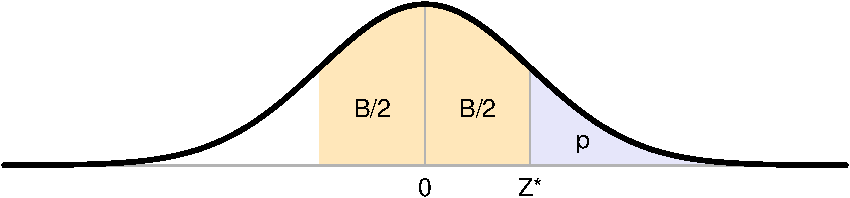
\includegraphics{KMS-NL_files/figure-latex/kritiekeZwaarden-hulpfiguur-1.pdf}

De hieronder gegeven kritieke grenswaarde \(Z^*\) heeft een overschrijdingskans \(p\) onder \(H_0\),
d.w.z. \(P(Z > Z^*|H_0)=p\) (de blauwe oppervlakte),
en heeft kans \(B\) op een waarde tussen \((-Z^*, +Z^*)\) (de gele oppervlakte).
De \(Z\)-verdeling is symmetrisch rond \(Z=0\), dus \(P(Z < -Z^*) = P(Z > Z^*)\).

\begin{center}\rule{0.5\linewidth}{0.5pt}\end{center}

De eerste tabel geeft de kritieke grenswaarden \(Z^*\) voor veel gebruikte overschrijdingskansen \(p\) en betrouwbaarheidsintervallen \(B\):

\begin{tabular}{ccccccccc}
\toprule
p & 0.2 & 0.1 & 0.05 & 0.025 & 0.01 & 0.005 & 0.0025 & 0.001\\
\midrule
B & 60\% & 80\% & 90\% & 95\% & 98\% & 99\% & 99.5\% & 99.8\%\\
Z* & 0.8416 & 1.282 & 1.645 & 1.960 & 2.326 & 2.576 & 2.807 & 3.090\\
\bottomrule
\end{tabular}

\begin{center}\rule{0.5\linewidth}{0.5pt}\end{center}

De tweede tabel geeft overschrijdingskansen \(p\) en betrouwbaarheidsintervallen \(B\) voor afgeronde kritieke grenswaarden \(Z^*\):

\begin{tabular}{cccccccc}
\toprule
p & 0.3085 & 0.1587 & 0.0668 & 0.0228 & 0.0062 & 0.0013 & 0.0002\\
\midrule
B & 38.29\% & 68.27\% & 86.64\% & 95.45\% & 98.76\% & 99.73\% & 99.95\%\\
Z* & 0.5 & 1 & 1.5 & 2 & 2.5 & 3 & 3.5\\
\bottomrule
\end{tabular}

\hypertarget{app:kritieketwaarden}{%
\chapter{\texorpdfstring{Kritieke waarden van \(t\)-verdeling}{Kritieke waarden van t-verdeling}}\label{app:kritieketwaarden}}

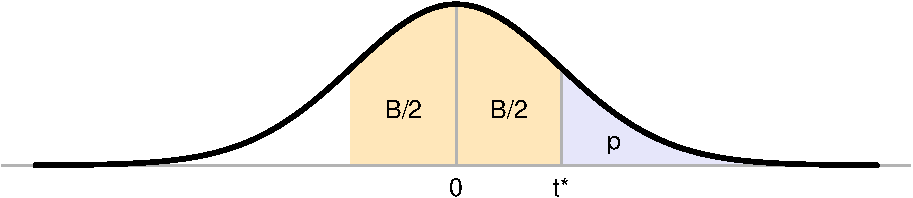
\includegraphics{KMS-NL_files/figure-latex/kritieketwaarden-hulpfiguur-1.pdf}

De hieronder gegeven kritieke grenswaarde \(t^*\) heeft een overschrijdingskans \(p\)
onder \(H_0\), d.w.z. \(P(t \geq t^*|H_0)=p\), en heeft kans \(B\) op een
waarde tussen \((-t^*, +t^*)\). De \(t\)-verdeling is symmetrisch rond
\(t=0\), dus \(P(t < -t^*) = P(t > t^*)\).

De tabel hieronder geeft de kritieke grenswaarden \(t^*\) voor veel gebruikte overschrijdingskansen \(p\) en betrouwbaarheidsintervallen \(B\), voor de vrijheidsgraden aangegeven in de eerste kolom.

\begin{tabular}{cccccccccc}
\toprule
 & p & 0.2 & 0.1 & 0.05 & 0.025 & 0.01 & 0.005 & 0.0025 & 0.001\\
\midrule
 & B & 60\% & 80\% & 90\% & 95\% & 98\% & 99\% & 99.5\% & 99.8\%\\
1 &  & 1.376 & 3.078 & 6.314 & 12.706 & 31.821 & 63.657 & 127.321 & 318.309\\
2 &  & 1.061 & 1.886 & 2.920 & 4.303 & 6.965 & 9.925 & 14.089 & 22.327\\
3 &  & 0.9785 & 1.638 & 2.353 & 3.182 & 4.541 & 5.841 & 7.453 & 10.215\\
4 &  & 0.941 & 1.533 & 2.132 & 2.776 & 3.747 & 4.604 & 5.598 & 7.173\\
\addlinespace
5 &  & 0.9195 & 1.476 & 2.015 & 2.571 & 3.365 & 4.032 & 4.773 & 5.893\\
6 &  & 0.9057 & 1.440 & 1.943 & 2.447 & 3.143 & 3.707 & 4.317 & 5.208\\
7 &  & 0.896 & 1.415 & 1.895 & 2.365 & 2.998 & 3.499 & 4.029 & 4.785\\
8 &  & 0.8889 & 1.397 & 1.860 & 2.306 & 2.896 & 3.355 & 3.833 & 4.501\\
9 &  & 0.8834 & 1.383 & 1.833 & 2.262 & 2.821 & 3.250 & 3.690 & 4.297\\
\addlinespace
10 &  & 0.8791 & 1.372 & 1.812 & 2.228 & 2.764 & 3.169 & 3.581 & 4.144\\
11 &  & 0.8755 & 1.363 & 1.796 & 2.201 & 2.718 & 3.106 & 3.497 & 4.025\\
12 &  & 0.8726 & 1.356 & 1.782 & 2.179 & 2.681 & 3.055 & 3.428 & 3.930\\
13 &  & 0.8702 & 1.350 & 1.771 & 2.160 & 2.650 & 3.012 & 3.372 & 3.852\\
14 &  & 0.8681 & 1.345 & 1.761 & 2.145 & 2.624 & 2.977 & 3.326 & 3.787\\
\addlinespace
15 &  & 0.8662 & 1.341 & 1.753 & 2.131 & 2.602 & 2.947 & 3.286 & 3.733\\
16 &  & 0.8647 & 1.337 & 1.746 & 2.120 & 2.583 & 2.921 & 3.252 & 3.686\\
17 &  & 0.8633 & 1.333 & 1.740 & 2.110 & 2.567 & 2.898 & 3.222 & 3.646\\
18 &  & 0.862 & 1.330 & 1.734 & 2.101 & 2.552 & 2.878 & 3.197 & 3.610\\
19 &  & 0.861 & 1.328 & 1.729 & 2.093 & 2.539 & 2.861 & 3.174 & 3.579\\
\addlinespace
20 &  & 0.860 & 1.325 & 1.725 & 2.086 & 2.528 & 2.845 & 3.153 & 3.552\\
21 &  & 0.8591 & 1.323 & 1.721 & 2.080 & 2.518 & 2.831 & 3.135 & 3.527\\
22 &  & 0.8583 & 1.321 & 1.717 & 2.074 & 2.508 & 2.819 & 3.119 & 3.505\\
23 &  & 0.8575 & 1.319 & 1.714 & 2.069 & 2.500 & 2.807 & 3.104 & 3.485\\
24 &  & 0.8569 & 1.318 & 1.711 & 2.064 & 2.492 & 2.797 & 3.091 & 3.467\\
\addlinespace
25 &  & 0.8562 & 1.316 & 1.708 & 2.060 & 2.485 & 2.787 & 3.078 & 3.450\\
30 &  & 0.8538 & 1.310 & 1.697 & 2.042 & 2.457 & 2.750 & 3.030 & 3.385\\
40 &  & 0.8507 & 1.303 & 1.684 & 2.021 & 2.423 & 2.704 & 2.971 & 3.307\\
50 &  & 0.8489 & 1.299 & 1.676 & 2.009 & 2.403 & 2.678 & 2.937 & 3.261\\
100 &  & 0.8452 & 1.290 & 1.660 & 1.984 & 2.364 & 2.626 & 2.871 & 3.174\\
\addlinespace
200 &  & 0.8434 & 1.286 & 1.653 & 1.972 & 2.345 & 2.601 & 2.839 & 3.131\\
400 &  & 0.8425 & 1.284 & 1.649 & 1.966 & 2.336 & 2.588 & 2.823 & 3.111\\
∞ &  & 0.8416 & 1.282 & 1.645 & 1.960 & 2.326 & 2.576 & 2.807 & 3.090\\
\bottomrule
\end{tabular}

\hypertarget{app:kritiekechi2waarden}{%
\chapter{\texorpdfstring{Kritieke waarden van \(\chi^2\)-verdeling}{Kritieke waarden van \textbackslash chi\^{}2-verdeling}}\label{app:kritiekechi2waarden}}

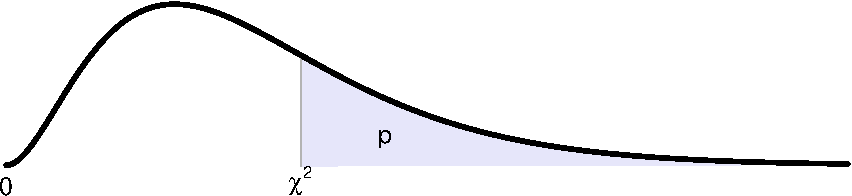
\includegraphics{KMS-NL_files/figure-latex/kritiekechi2waarden-hulpfiguur-1.pdf}

De hieronder gegeven kritieke grenswaarde \((\chi^2)^*\) heeft een overschrijdingskans \(p\)
onder \(H_0\), d.w.z. \(P(\chi^2 \geq (\chi^2)^*|H_0)=p\).

De tabel hieronder geeft de kritieke grenswaarden \((\chi^2)^*\) voor veel gebruikte overschrijdingskansen \(p\), voor de vrijheidsgraden aangegeven in de eerste kolom.

\begin{tabular}{cccccccccc}
\toprule
 & p & 0.2 & 0.1 & 0.05 & 0.025 & 0.01 & 0.005 & 0.0025 & 0.001\\
\midrule
1 &  & 1.64 & 2.71 & 3.84 & 5.02 & 6.63 & 7.88 & 9.14 & 10.83\\
2 &  & 3.22 & 4.61 & 5.99 & 7.38 & 9.21 & 10.60 & 11.98 & 13.82\\
3 &  & 4.64 & 6.25 & 7.81 & 9.35 & 11.34 & 12.84 & 14.32 & 16.27\\
4 &  & 5.99 & 7.78 & 9.49 & 11.14 & 13.28 & 14.86 & 16.42 & 18.47\\
5 &  & 7.29 & 9.24 & 11.07 & 12.83 & 15.09 & 16.75 & 18.39 & 20.52\\
\addlinespace
6 &  & 8.56 & 10.64 & 12.59 & 14.45 & 16.81 & 18.55 & 20.25 & 22.46\\
7 &  & 9.80 & 12.02 & 14.07 & 16.01 & 18.48 & 20.28 & 22.04 & 24.32\\
8 &  & 11.03 & 13.36 & 15.51 & 17.53 & 20.09 & 21.95 & 23.77 & 26.12\\
9 &  & 12.24 & 14.68 & 16.92 & 19.02 & 21.67 & 23.59 & 25.46 & 27.88\\
10 &  & 13.44 & 15.99 & 18.31 & 20.48 & 23.21 & 25.19 & 27.11 & 29.59\\
\addlinespace
11 &  & 14.63 & 17.28 & 19.68 & 21.92 & 24.72 & 26.76 & 28.73 & 31.26\\
12 &  & 15.81 & 18.55 & 21.03 & 23.34 & 26.22 & 28.30 & 30.32 & 32.91\\
13 &  & 16.98 & 19.81 & 22.36 & 24.74 & 27.69 & 29.82 & 31.88 & 34.53\\
14 &  & 18.15 & 21.06 & 23.68 & 26.12 & 29.14 & 31.32 & 33.43 & 36.12\\
15 &  & 19.31 & 22.31 & 25.00 & 27.49 & 30.58 & 32.80 & 34.95 & 37.70\\
\addlinespace
16 &  & 20.47 & 23.54 & 26.30 & 28.85 & 32.00 & 34.27 & 36.46 & 39.25\\
17 &  & 21.61 & 24.77 & 27.59 & 30.19 & 33.41 & 35.72 & 37.95 & 40.79\\
18 &  & 22.76 & 25.99 & 28.87 & 31.53 & 34.81 & 37.16 & 39.42 & 42.31\\
19 &  & 23.90 & 27.20 & 30.14 & 32.85 & 36.19 & 38.58 & 40.88 & 43.82\\
20 &  & 25.04 & 28.41 & 31.41 & 34.17 & 37.57 & 40.00 & 42.34 & 45.31\\
\addlinespace
21 &  & 26.17 & 29.62 & 32.67 & 35.48 & 38.93 & 41.40 & 43.78 & 46.80\\
22 &  & 27.30 & 30.81 & 33.92 & 36.78 & 40.29 & 42.80 & 45.20 & 48.27\\
23 &  & 28.43 & 32.01 & 35.17 & 38.08 & 41.64 & 44.18 & 46.62 & 49.73\\
24 &  & 29.55 & 33.20 & 36.42 & 39.36 & 42.98 & 45.56 & 48.03 & 51.18\\
25 &  & 30.68 & 34.38 & 37.65 & 40.65 & 44.31 & 46.93 & 49.44 & 52.62\\
\addlinespace
30 &  & 36.25 & 40.26 & 43.77 & 46.98 & 50.89 & 53.67 & 56.33 & 59.70\\
40 &  & 47.27 & 51.81 & 55.76 & 59.34 & 63.69 & 66.77 & 69.70 & 73.40\\
50 &  & 58.16 & 63.17 & 67.50 & 71.42 & 76.15 & 79.49 & 82.66 & 86.66\\
100 &  & 111.67 & 118.50 & 124.34 & 129.56 & 135.81 & 140.17 & 144.29 & 149.45\\
200 &  & 216.61 & 226.02 & 233.99 & 241.06 & 249.45 & 255.26 & 260.74 & 267.54\\
\addlinespace
400 &  & 423.59 & 436.65 & 447.63 & 457.31 & 468.72 & 476.61 & 483.99 & 493.13\\
\bottomrule
\end{tabular}

  \bibliography{book.bib,packages.bib,hhmhto.bib,pandoc.bib}

\end{document}
